\documentclass[a4paper,11pt]{book}

% Import package settings.
\usepackage{syntonly}
% \syntaxonly

% \usepackage{indentfirst}
% \setlength{\parindent}{2em}
% -or-
\usepackage[parfill]{parskip}

\usepackage{hyperref}

% style=ieee-alphabetic
\usepackage[backend=biber,style=ieee]{biblatex}
\addbibresource{biblatex.bib}

\usepackage{graphicx}
\graphicspath{{./figs/}{./}}
\usepackage{subcaption}

% \usepackage{lscape} % PDF page contents landscape
\usepackage{pdflscape} % PDF page landscape

\usepackage[toc,page]{appendix}

\usepackage{amsmath}
\usepackage{amssymb}
\usepackage{mathtools}

\usepackage{multicol}

\usepackage{pgfplotstable}
\usepackage{booktabs}

\usepackage[round-mode=places,round-precision=3]{siunitx}

\usepackage{pgfplots}
\pgfplotsset{compat=newest} % Allows to place the legend below plot
\usepgfplotslibrary{units} % Allows to enter the units nicely

% draw math injection
\usepackage[all]{xypic}

% draw diagonally divided table cell
% \usepackage{slashbox} % ancient and deprecated
\usepackage{diagbox}

% add underline to text
\usepackage{ulem}

% chemical equations
\usepackage[version=4]{mhchem}

% insert PDF page
\usepackage{pdfpages}


%%% Local Variables:
%%% mode: latex
%%% TeX-master: "main"
%%% End:

\usepackage{fontspec}

% Western fonts by 'fontspec':
\setmainfont{Tinos}[ % search font by filename
  Path = /opt/fonts/core/Tinos/,
  Extension = .ttf,
  UprightFont = *-Regular,
  BoldFont = *-Bold,
  ItalicFont = *-Italic,
  BoldItalicFont = *-BoldItalic
]
\setsansfont{NotoSans}[ % search by 'postscriptname'
  BoldFont = NotoSans-Bold,
  ItalicFont = NotoSans-Italic,
  BoldItalicFont = NotoSans-BoldItalic  
]
\setmonofont{migu-1m-regular}[
  BoldFont = migu-1m-bold
]

% Chinese fonts by 'fontspec':
%
% \setmainfont{Adobe Song Std}
% \setsansfont{Noto Sans S Chinese}
% \setmonofont{Adobe Fangsong Std}
% \XeTeXlinebreaklocale "zh"
% \XeTeXlinebreakskip = 0pt plus 1pt minus 0.1pt
% \usepackage[top=1in,bottom=1in,left=1.2in,right=1in]{geometry}


% Chinese fonts by 'xeCJK':
\usepackage[boldfont]{xeCJK}
\setCJKmainfont{Adobe Song Std}[ % search by 'family'
BoldFont = NotoSansHans-Bold % search by 'postscriptname'
                             % because 'NotoSansHans' family has
                             % multiple variants.
]
\setCJKsansfont{NotoSansHans-DemiLight}[
  BoldFont = NotoSansHans-Bold
]
\setCJKmonofont{Adobe Fangsong Std}

% set new font family
\setCJKfamilyfont{zhyahei}{msyh}[ % search font by filename
  Path = fonts/,
  Extension = .ttf,
  BoldFont = {*bd}
]
% create font family command alias
\NewDocumentCommand{\yahei}{}{\CJKfamily{zhyahei}}


% Chinese fonts by 'xeCJK' from 'CTeX':
%
% \usepackage[UTF8,heading=true]{ctex}

% \setcjkmainfont{Adobe Song Std} % search by `family'
% \setCJKsansfont{NotoSansHans-DemiLight}[
%   BoldFont = NotoSansHans-Bold
% ]
% \setCJKmonofont{Adobe Fangsong Std}

%%% Local Variables:
%%% mode: latex
%%% TeX-master: "main"
%%% End:

\usepackage{listings}
\usepackage{color}

\definecolor{mygreen}{rgb}{0,0.6,0}
\definecolor{mygray}{rgb}{0.5,0.5,0.5}
\definecolor{mymauve}{rgb}{0.58,0,0.82}

\lstset{                           % default settings; you should override at least 'language' part when typesetting
  backgroundcolor=\color{white},   % choose the background color; you must add \usepackage{color} or \usepackage{xcolor}; should come as last argument
  basicstyle=\footnotesize\ttfamily,        % the size of the fonts that are used for the code
  breakatwhitespace=false,         % sets if automatic breaks should only happen at whitespace
  breaklines=true,                 % sets automatic line breaking
  captionpos=b,                    % sets the caption-position to bottom
  columns=flexible,
  commentstyle=\color{mygreen},    % comment style
  deletekeywords={},               % if you want to delete keywords from the given language
  escapeinside={\%*}{*)},          % if you want to add LaTeX within your code
  extendedchars=true,              % lets you use non-ASCII characters; for 8-bits encodings only, does not work with UTF-8
  frame=single,	                   % adds a frame around the code
  keepspaces=true,                 % keeps spaces in text, useful for keeping indentation of code (possibly needs columns=flexible)
  keywordstyle=\color{blue},       % keyword style
  language=TeX,                      % the language of the code
  morekeywords={},                 % if you want to add more keywords to the set
  numbers=left,                    % where to put the line-numbers; possible values are (none, left, right)
  numbersep=5pt,                   % how far the line-numbers are from the code
  numberstyle=\tiny\color{mygray}, % the style that is used for the line-numbers
  rulecolor=\color{black},         % if not set, the frame-color may be changed on line-breaks within not-black text (e.g. comments (green here))
  showspaces=false,                % show spaces everywhere adding particular underscores; it overrides 'showstringspaces'
  showstringspaces=false,          % underline spaces within strings only
  showtabs=false,                  % show tabs within strings adding particular underscores
  stepnumber=2,                    % the step between two line-numbers. If it's 1, each line will be numbered
  stringstyle=\color{mymauve}\ttfamily,     % string literal style
  tabsize=4,	                   % sets default tabsize to 2 spaces
  title=\lstname,                  % show the filename of files included with \lstinputlisting; also try caption instead of title
  xleftmargin=.05\textwidth,        % show 'lstlisting' at page center
  xrightmargin=.05\textwidth
}

%%% Local Variables:
%%% mode: latex
%%% TeX-master: "main"
%%% End:


% Tell `include' to only include these sources in the body.
\includeonly{preface,resources,chinese,tutorial,
  combinatorics,sequenceOfNumber,
  terminologies,os,dns,http,ictOP,
  tree,stack,regex,
  bash,c,cpp,python,
  tcpIP,dataBills,netools,
  brainteaser,aat,
  chemistry,
  appendices,postscript}

\begin{document}

\frontmatter{}

\title{ICT}
\author{西二闲画话\\
  Department of Life,\\
  Zhonghua Uni.,\\
  Wuhan, China\\
  \emph{zhu@riseup.net}}
\date{\today}
\maketitle


\chapter{Preface}
\label{cha:preface}

\LaTeX{} typesets text as \textit{What You See Is What You Type}
compared with \textit{What You See Is What You Get}. It gives
finer control over text layout with a host of commands and
add-ons. This book firstly demonstrates how \LaTeX{} supports
Chinese typesetting and then moves on to syntax. A bit of ACTeX
with Emacs configuration and key bindings are dicussed as
well. Gradually, topics from different disciplines (i.e. math and
language) are introduced in separate parts.

Priorly, I just planned to learn \LaTeX{} through trial and
error. As it progressed, I found \LaTeX{} an awesome typesetting
tool, creating beautiful text output. Hence, I decided to make
it a book containing different parts, covering formal subjects
like math, physics, etc. Ultimately, I want to maintain a
centralized offline jottings which can be testified by the book
title \textit{Miscellanies}.

%%% Local Variables:
%%% mode: latex
%%% TeX-master: "main"
%%% End:


\setcounter{tocdepth}{3} % Show subsubsections
\tableofcontents{}

\mainmatter{}

\part{\LaTeX{}}
\chapter{\LaTeX{} Resources}
\label{cha:latex-resources}

\section{Find References}
\label{sec:find-references}

In part \ref{cha:inputChinese} on page
\pageref{cha:inputChinese}, we have a simple clarification on
how to insert Chinese characters in English articles. We will
focus on \LaTeX{} itself in this part.

Please find more appropriate at
\href{https://ctan.org/topic/tut-latex?lang=en}{\LaTeX{}
  ctan}. Also, please find anwsers at
\cite{stackexchange}. You'd better go through the tutorial series
\cite{tutorial}. My personal webiste \cite{zhstar} might give some
ideas.

\section{AUCTeX}
\label{sec:auctex}

\subsection{Inserting}
\label{sec:inserting}

\begin{table}[tbp]
  \centering
  \begin{tabular}{|l|l|}
    \hline{}
    Binding & Function \\ \hline \hline{}
    \verb|C-c C-e| & insert environment \\ \hline{}
    \verb|C-c C-s| & insert section \\ \hline{}
    \verb|C-c C-m| & macro (command) \\ \hline{}
    \verb|M-return| & another item \\ \hline{}
    \verb|C-c C-c| & compile \LaTeX{} \\ \hline{}
    \verb|C-c C-v| & preview output \\ \hline{}
    \verb|C-c =| & show document layout by RefTeX \\ \hline{}
    \verb|C-c C-o C-b| & fold the buffer \\ \hline{}
    \verb|C-c C-o b| & unfold the buffer \\ \hline{}
    \verb|C-c C-r| & compile selected region \\ \hline{}
    \verb|C-c C-b| & compile current buffer \\ \hline
  \end{tabular}
  \caption{AUCTeX Bindings}
  \label{tab:auctex-bindings}
\end{table}

Have a look at
\href{https://github.com/bigclean/blogs/blob/master/emacs/auctex.mkd}{\LaTeX{}}

\subsection{\LaTeX{} Sources Formating}
\label{sec:code-formating}

Use \verb|C-c C-q C-s| to format \LaTeX{} \textit{section}
code. \verb|C-c C-q C-p| is to format \textit{paragraph} text.

\subsection{Font Specifiers}
\label{sec:font-specifiers}

Use \verb|C-c C-f C-i| to insert \textit{italic} text. Smililary,
Use \verb|C-c C-f C-b| to insert \textit{bold} text. Read more at \href{https://www.gnu.org/software/auctex/manual/auctex/Font-Specifiers.html}{Insert Font Spcecifiers}.

\begin{center}
  \begin{tabular}{|l|l|}
    \hline{}
    C-c C-f C-i	& italic \\ \hline{}
    C-c C-f C-b & bold \\ \hline{}
    C-c C-f C-e & emphasize \\ \hline{}
    C-c C-f C-s & slight italic \\ \hline{}
    C-c C-f C-r & roman \\ \hline{}
    C-c C-f C-f & sans \\ \hline{}
    C-c C-f C-d & delete font formating \\ \hline
  \end{tabular}
\end{center}

%%% Local Variables:
%%% mode: latex
%%% TeX-master: "main"
%%% End:

\chapter{汉语}
\label{cha:inputChinese}

对字体的引用要注意,如果一个字体族 family 有多个变种 \footnote{如
  regular, bold, italic 等。},请引用字体的 postscriptname.

默认情况下,\LaTeX{} 会把文档里用到的字体子集内嵌到生成的 PDF 里,
可以通过命令行 \textit{pdffonts filename.pdf} 查询,结果
如 \ref{cha:too-big-fit} 所示。

此例说明,对应文档内嵌了七个字体子集。\LaTeX{} 文档通常只会用到字
体文件的部分 code point,所以只需要内嵌使用到的部分即可。每个字体
的前面都有一串无规则字母,代表对应字体文件被内嵌的子集。还有一列叫
sub 也说明是否是子集。

\section{CJK 包}

在英文文档里插入少量中文

\subsection{CJK 和 CJK* 环境}
在英文文档里用 CJK 包的 CJK 或 CJK* 环境插入少量汉字。后者会忽略汉
字后面的空格,推荐使用。

\subsection{字体}
bsmi~字体可能没有,尝试换一个如~gkai, ~gbsn~等。

\section{xeCJK 更好}
xeCJK 在处理细节上更好,关键是可方便设置中英文字体。用 xeCJK 则不需
要特殊环境包裹汉字,只需在``导言区''设置好中英文字体即可。

xeCJK 的 indentfirst 选项:
\begin{center}
  \verb|\usepackage[indentfirst]{xeCJK}|
\end{center}
已过时,推荐直接用 indentfirst 宏包:
\begin{center}
  \verb|\usepackage{indentfirst}|
\end{center}

\section{fontspec 和 ctex}
\label{sec:fontspec-ctex}

还有 \textit{fontspec} 和 \textit{ctex} 包可以实现中文输入,更多详
情请看 \href{https://www.zhstar.win/2015/02/05/LaTeX/}{\LaTeX{}
  post}.

\begin{itemize}
\item \verb|fontspec| sets western or Chinese fonts (i.e. main, sans, serif, bold, italic, and bolditalic).
\item \verb|CJK| sets Chinese, Japanese, and Korean fonts, punctuation etc. for TeX engine.
\item \verb|xeCJK| similar to \verb|CJK| but for XeTeX engine.
\item \verb|CTeX| sets \verb|CJK/xeCJK| document layout.
\end{itemize}

\section{中英文空格}
我们想要的效果是英文字符前后自动加上空格。xeCJK 则会自动处理,但是
效果不是非常好。

CJK 会忽略 \TeX{} 源码里的空格。用 CJK 宏集里的 CJKspace 包,源码里
英文后空格会保留,中文后空格依然被 CJK* 压缩。还有一个方法是在需要空
格的地方用 tilde $\sim$.

\section{行首缩进}

中文习惯每段行首缩进两个汉字。英文有两种缩进格式。默认是每小节的第
一段缩进,后面的段不缩进,段间没有空行。另一种是不缩进,每段间留有
空行。

本文档只插入少量中文作例子,固保留英文默认缩进方式。如要换成中文缩
进,则用 indentfirst 包,使每节第一段也缩进,如下:
\begin{center}
  \begin{tabular}{l}
    \verb|\usepackage{indentfirst}| \\
    \verb|\setlength{\parindent}{2em}|
  \end{tabular}
\end{center}
如若换成英文第二种缩进,则
用\href{https://tex.stackexchange.com/a/40432}{parskip} 包,skip 表
示相临两段之间的间隙大小:
\begin{center}
  \begin{tabular}{l}
    \verb|\usepackage[parfill]{parskip}|
  \end{tabular}
\end{center}
也可用相对应的命令实现:
\begin{center}
  \begin{tabular}{l}
    \verb|\setlength{\parindent}{0pt}| \\
    \verb|\setlength{\parskip}{1ex plus 0.5ex minus 0.2ex}|
  \end{tabular}
\end{center}

\section{局部字体命令}

前面提到的方法都是全局生效,有没有类似 \verb|\emph{}| 和
\verb|\textit{}| 这种监时改中文字体的方法呢?

在 \textit{xecjk.tex} 中有如下代码:

\begin{lstlisting}[language=TeX,caption={New font family},label={lst:new-font-family}]
% set new font family
\setCJKfamilyfont{zhyahei}{msyh}[
  Path = fonts/,
  Extension = .ttf,
  BoldFont = {*bd}
]

% create font family command alias
\NewDocumentCommand{\yahei}{}{\CJKfamily{zhyahei}}
\end{lstlisting}

根据需求定义一个新的字体族 family 名 \textit{zhyahei},新字体族的
引用方法是:

\begin{lstlisting}[language=TeX,caption={Inline Chinese fonts},label={lst:inline-chn-fonts}]
{\CJKfamily{zhyahei}{这里输中文}}
% -or-
{\CJKfamily{zhyahei}这里输中文}
\end{lstlisting}

为了方便,我们还定义一个新 NewDocumentCommand 命令,便于快速引
用。\verb|{\yahei{这是新定义的雅黑字体样例。}}| 的效果
如:{\yahei{这是新定义的雅黑字体样例。}}

特别注总,命令要放在一个 group 里,即用 \verb|{}| 围起来,否则从当
前位置起,所有中文字体都改了。实际,fontspec 提供类似功能,具体请参
考 fontspec 文档。如:

\begin{center}
  \verb|\fontspec{⟨font name⟩}[⟨fontfeatures⟩]| 和 \verb|\newfontfamily|
\end{center}


%%% Local Variables:
%%% mode: latex
%%% TeX-master: "main"
%%% End:

\chapter{\LaTeX{} Tutorial}
\label{cha:latex-tutorial}

\section{\TeX{} Units}
\label{sec:tex-units}

\begin{figure}[h]
  \centering
  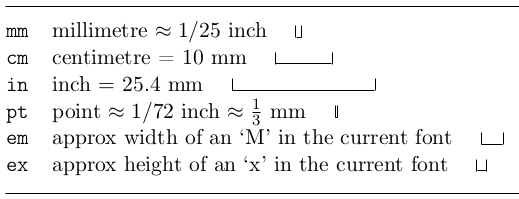
\includegraphics[width=.5\textwidth]{units}
  \caption{\TeX{} Units}
  \label{fig:tex-units}
\end{figure}

\section{Special characters}
\label{sec:special-characters}

The following 10 characters has special meanings in
\LaTeX{}.

\begin{center}
  \verb|& % $ # _ { } ~ ^ \|
\end{center}

Outside \textit{verb}, the first 7 should escaped by
\textit{backslash}. Of the last three, we use \LaTeX{} macros,
namely \verb|\textasciitilde|, \verb|\textasciicircum| and
\verb|\textbackslash|.

\begin{lstlisting}[language=TeX,caption={Special Characters},label={lst:special-characters}]
\& \% \$ \# \_ \{ \} \textasciitilde{} \textasciicircum{} \textbackslash{}
\end{lstlisting}

Specially, \LaTeX{} uses tilde \textasciitilde{} as a non-breaking space. You
would usually use non-breaking spaces for punctuation marks in
some languages, for units and currencies, for initials, etc.

\section{verbatim and verb}
\label{sec:verbatim-verb}

When to show raw text without \LaTeX{} command being executed, use
\textit{verbatim} environment or \textit{verb} command. Both have
an asterisk alternative like \verb|\begin{verbatim*}| and
  \verb|\verb*|. With extra *, \LaTeX{} will typewrite space as
\texttt{␣}.

You can't use \texttt{\textbackslash{}verb} in other command's
parameters. For example, this is not allowed:

\begin{lstlisting}[language=TeX,caption={Illegal verb}]
\href{https://tex.stackexchange.com/a/23653}{When should we use
  \verb|\begin{center}| instead of \verb|\centering|?}
\end{lstlisting}

Instead, we use
\href{https://tex.stackexchange.com/q/2790}{\texttt{\textbackslash{}texttt}}
and escape special characters \footnote{For instance, backslash
and \{.} like:

\begin{lstlisting}[language=TeX,caption={texttt}]
\href{https://tex.stackexchange.com/a/23653}{When should we use
\texttt{\textbackslash{}begin\{center\}} instead of \texttt{\textbackslash{}centering}?}
\end{lstlisting}

\section{item list}
\label{sec:item-list}

Using lists is quite straightforward and does not require you to
add any additional packages. For unordered list, \LaTeX{} provides
the \textit{itemize} environment and for ordered list there is the
\textit{emunerate} environment. With both environments, elements
should be declared beginning with \verb|\item| command. We can use
\verb|M-Enter| binding to insert this command automatically.

Take a look at unordered list\ref{lst:itemize-unordered-list}:

\begin{minipage}{.4\linewidth}
\begin{lstlisting}[label={lst:itemize-unordered-list},linewidth=.7\textwidth]
\begin{itemize}
\item One
\item HKUST
\item HUST
\end{itemize}
\end{lstlisting}  
\end{minipage}
\hfill
\framebox{
\begin{minipage}{0.4\linewidth}
  \begin{itemize}
  \item One
  \item HUST
  \item HKUST
  \end{itemize}
\end{minipage}
}

Here is an ordered list \ref{lst:enumerate-ordered-list}:

\begin{minipage}{.4\linewidth}
  \begin{enumerate}
  \item Jim
  \item Gray
    \begin{itemize}
    \item This is a
    \item nested unordered
    \item list within ordered list
    \end{itemize}
  \item Who are you?
  \end{enumerate}
\end{minipage}
\hfill{}
\begin{minipage}{.4\linewidth}
\begin{lstlisting}[label={lst:enumerate-ordered-list}]
\begin{enumerate}
\item Jim
\item Gray
  \begin{itemize}
  \item This is a
  \item nested unordered
  \item list within ordered list
  \end{itemize}
\item Who are you?
\end{enumerate}
\end{lstlisting}
\end{minipage}

\section{Code listings}
\label{sec:code-listings}

Although \textit{verb} and \textit{verbatim} enclose raw text,
they don't highlight source code like C, Java etc. This is where
\textit{listings} package come into
\href{https://en.wikibooks.org/wiki/LaTeX/Source_Code_Listings}{usage}.

To insert a code block, use \textit{lstlisting} environment like

\begin{center}
  \verb|\begin{lstlisting}[language=bash,caption={Bash},frame=single]|
\end{center}

Here is an example:

\begin{lstlisting}[language=bash,caption={Bash},frame=single]
#!/bin/bash
echo 'Hello, world!'
\end{lstlisting}

Furthermore,
\begin{lstlisting}[language=TeX,caption={Include code file},breaklines]
\lstinputlisting[language=C,frame=tb,basicstyle=\scriptsize\ttfamily]{helloworld.c}
\end{lstlisting}
command includes code source file:
\lstinputlisting[language=C,frame=single,
caption={C98}]{helloworld.c} This is useful when the code needs
updating frequently.

To prevent \textit{lstlisting} from breaking pages, we should wrap
it within \textit{minipage} environment as \ref{lst:table-floating}.

Sometimes, code line is too long to fit page width, leaving
tailing part out of page. We could modify \textit{basicstyle} to
one of \textit{footnotesize}, \textit{scriptsize} and
\textit{tiny}. Check long text line example
\ref{cha:too-big-fit}. For more options, read
\href{https://tug.org/texinfohtml/latex2e.html#Font-sizes}{Font
  Size} and \href{https://tex.stackexchange.com/q/24599}{font size
  and point (pt) relation}.

{\LARGE This is LARGE text} {\Huge while this is Huge}.

\section{Straight Quotes}
\label{sec:straight-quotes}

By default, \textit{listings} typesets both single and double as
\textit{back curve ones}.

We should import \textit{textcomp} package and \textit{fontenc}
package with \href{https://tex.stackexchange.com/a/677}{T1}
option. Then, enable \textit{upquote=true} for code block. Read
more at \href{https://tex.stackexchange.com/q/166790}{How can I
  get straight double quotes in listings?}

This method, however, is discouraged as \textit{fontenc} would
override the whole document \LaTeX{} font settings. The underlying
cause is \textit{serif (roman)} font. Default roman fonts does not
provide straight quotes. We should tell \textit{listings} to use
\textit{monospace} font instead by

\begin{center}
  \verb|\lstset{basicstyle=\ttfamily}|
\end{center}

Read more at
\href{https://tex.stackexchange.com/q/144396}{Consolas: Straight
  Quotes}.

\section{floating}
\label{sec:floating}

\subsection{Figure}
\label{sec:figure}

First, we import \textit{graphicx} package and then set
\textit{graphicspath} in preamble part:
\begin{lstlisting}[language=TeX,caption={graphicx}]
\usepackage{graphicx}
\graphicspath{{figs/}{./}}
\end{lstlisting}

\textit{graphicx} accepts EPS, PDF, PNG or JPEG
formats. \textit{graphicspath} defines a list of directories
relative to that of \textit{master.tex}. By this means, we can
access images anywhere without restriction like
\verb|\graphicspath{{../../img/}}|. The trailing slash cannot be
omitted.

Then, we use command \textit{includegraphics} like

\begin{center}
  \verb|\includegraphics[width=.5\textwidth,scale=0.1]{myimg}|
\end{center}

Notice that we do not write figure file extension. Here is the
output:
\begin{center}
  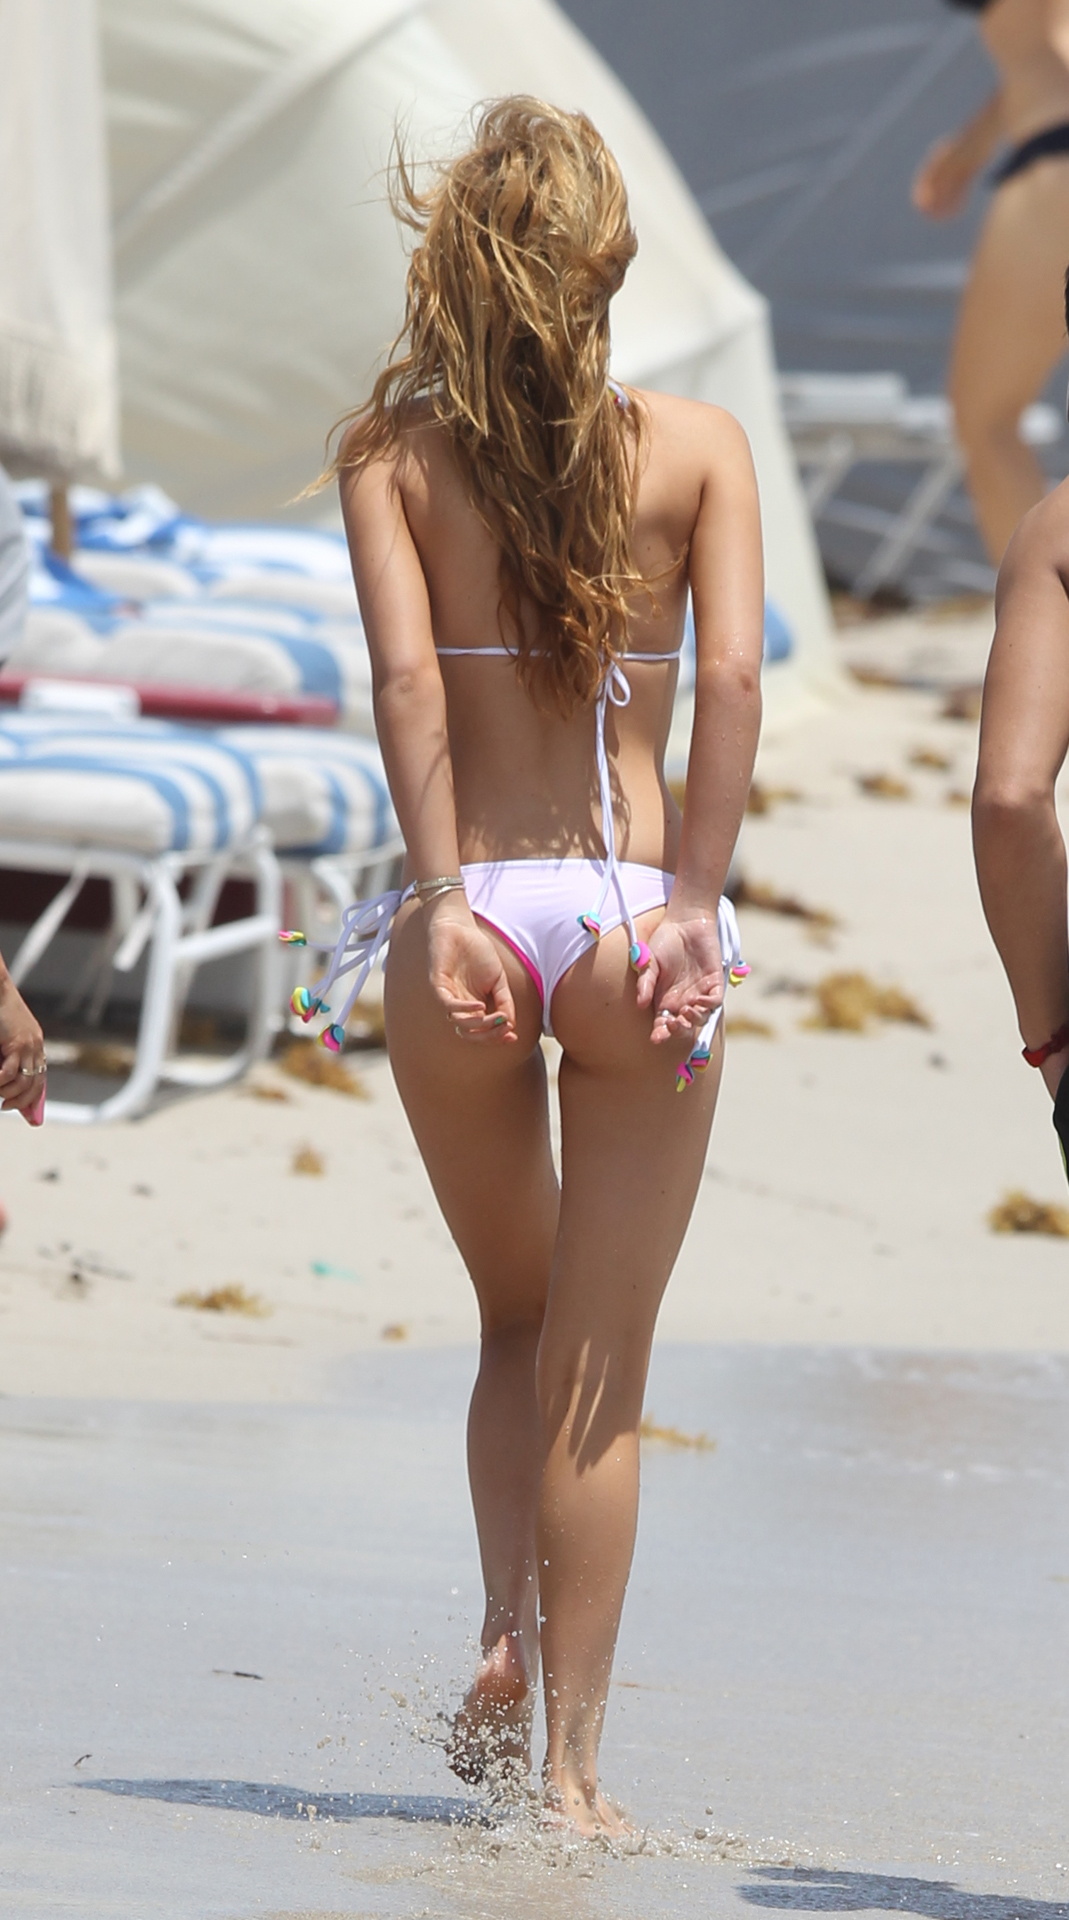
\includegraphics[width=.5\textwidth,scale=0.1]{leg}
\end{center}

With bare \textit{includegraphics}, if remaining space within current
page does not hold the figure, \LaTeX{} would start a new page
instead, leaving current page partially emtpy. The method is to
wrap it with \textit{figure} environment:

\begin{minipage}[top]{1.0\linewidth}
\begin{lstlisting}[language=TeX,caption={Figure Floating}]
\begin{figure}[tbp]
  \centering
  \includegraphics[width=\textwidth]{Boobs}
  \caption{Boobs}
  \label{fig:Boobs}
\end{figure}
\end{lstlisting}  
\end{minipage}

We call this technique as \textit{floating}. Apart from
\textit{placement specifier} benefits, we can define
\textit{label} and \textit{caption} within \textit{floating}
environment. Note that \verb|\label{}| command must come
\textbf{after} \verb|\caption{}| command since the reference
number is generated by \verb|\caption{}|. For details, refer to
\href{https://tex.stackexchange.com/a/32326}{Why does an
  environment's label have to appear after the caption?}.

The \verb|tbp| \footnote{\textit{tbp} is the default
  \textit{placement specifier}. We could set it to
  \textit{!htbp}.} specifies position of floating environment.

\begin{figure}[h]
  \centering
  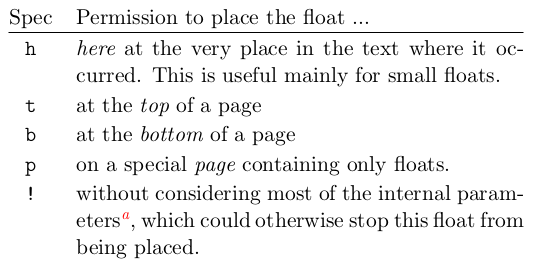
\includegraphics[width=.5\textwidth]{floating}
  \caption{Floating Placement Specifiers}
  \label{fig:placement-specifiers}
\end{figure}

Here is a nice boobs example \ref{fig:boobs}:

\begin{figure}[!htbp]
  \centering
  
\includegraphics[scale=.3]{boobs}
  \caption{boobs}
  \label{fig:boobs}
\end{figure}

Sometimes, it's necessary to put figures side by side for clear
comparasion. We use \textit{subfigure} within \textit{figure} like
\ref{fig:three-girsl}. Please be noted that we add non-breakable
symbol \textasciitilde{} between \textit{subfigure} to leave
some space between figures.

\begin{figure}[tbp]
  \centering
  \begin{subfigure}[tbp]{0.3\linewidth}
    
\includegraphics[width=\linewidth]{sub1}
    \caption{Girl A}
  \end{subfigure}
  ~
  \begin{subfigure}[tbp]{0.3\linewidth}
    
\includegraphics[width=\linewidth]{sub2}
    \caption{Girl B}
  \end{subfigure}
  ~
  \begin{subfigure}[tbp]{0.3\linewidth}
    
\includegraphics[width=\linewidth]{sub3}
    \caption{Girl C}
  \end{subfigure}
  \caption{Three Girls}
  \label{fig:three-girsl}
\end{figure}

\subsection{Table}
\label{sec:table}

Similarly, we can wrap \textit{tabular} within \textit{table}
environment to \textit{float} table \ref{tab:auctex-bindings} like
\ref{lst:table-floating}.

\begin{minipage}[top]{1.0\linewidth}
\begin{lstlisting}[language=TeX,caption={Table Floating},label={lst:table-floating}]
\begin{table}[!htbp]
  \centering
  \begin{tabular}{|l|r|}
    \hline{}
    Binding & Function \\ \hline \hline{}
    \verb|C-c C-e| & insert environment \\ \hline{}
    \verb|C-c C-s| & insert section \\ \hline{}
    \verb|C-c C-m| & macro (command) \\ \hline{}
    \verb|M-return| & another item \\ \hline{}
    \verb|C-c C-c| & compile \LaTeX{} \\ \hline{}
    \verb|C-c C-v| & preview output \\ \hline{}
    \verb|C-c =| & show document layout by RefTeX \\ \hline{}
    \verb|C-c C-o C-b| & fold the buffer \\ \hline{}
    \verb|C-c C-o b| & unfold the buffer \\ \hline
  \end{tabular}
  \caption{AUCTeX Bindings}
  \label{tab:auctex-bindings}
\end{table}
\end{lstlisting}
\end{minipage}

In \textit{tabular} environment, we align column texts as
\textit{\textbf{l}eft}, \textit{\textbf{c}enter} and
\textit{\textbf{r}ight}. What about decimal number cell? Idealy,
we want to align numbers at dot, where package \textit{siunitx}
plays a role by \textbf{S} \ref{tab:number-alignment-at-dot}
alignment specifier.

\begin{lstlisting}[language=TeX,caption={Decimal Alignment},label={lst:decimal-alignment}]
\usepackage[round-mode=places,round-precision=3]{siunitx}
\end{lstlisting}

To make prettier table, we use package \textit{booktabs} which
provides \textit{toprule}, \textit{midrule} and
\textit{bottomrule} to override \footnote{It is not replace!} dull \textit{hline}.

\begin{table}[tbp]
  \centering
  \begin{tabular}{l|S|r}
    \toprule{}
    \textbf{List 1} & \textbf{Decimal 2} & \textbf{Letter 3} \\
    $\alpha$ & $\beta$ & $\gamma{}$ \\
    \midrule{}
    1 & 1385.1 & a \\
    2 & 3.0674 & b \\
    3 & 87.369 & c \\
    \bottomrule
  \end{tabular}
  \caption{Number Alignment at Dot}
  \label{tab:number-alignment-at-dot}
\end{table}

To make more complex tables, we can use package \textit{multirow}
and \textit{multirow} and \textit{multicolumn} environment
respectivelly.

When typesetting large tables, it is tedious and error-prone which
could be avoided by \textit{pgfplotstable} package that generate
tables from external \textit{.csv} file. Programs such as Excel,
OpenOffice Calc or even emacs org-mode can export data sheets as
\textit{.csv} files. The \textit{pgfplotstable template}
\ref{sec:pgfplotstable-template} generate table
\ref{table-automation-from-csv}.

\begin{table}[tbp]
  \centering{}
  \pgfplotstabletypeset[
    multicolumn names,
    col sep=comma,
    display columns/0/.style={
      column name=$Ampere$,
      column type={S},string type
    },
    display columns/1/.style={
      column name=$Voltage$,
      column type={S},string type
    },
    display columns/2/.style={
      column name=$Energy$,
      column type={S},string type
    },
    every head row/.style={
      before row={\toprule},
      after row={
        \si{\ampere} & \si{\volt} & \si{\joule} \\
        \midrule
      }
    },
    every last row/.style={
      after row=\bottomrule
    },
  ]{pgfplotstable.csv}
  \caption{Table automation from .csv file.}
  \label{table-automation-from-csv}
\end{table}

\subsection{Plot}
\label{sec:plot}

The \textit{pgfplots} package is a powerful tool, based on
\textit{tikz} package, dedicated to create scientific
graphs. Similar to \textit{pgfplotstable}, \textit{pgfplots} can
read date from \textit{.csv} file.

Since \textit{pgfplots} is based on \textit{tikz}, the
\textit{axis} environment should be enclosed within
\textit{tikzpicture} environment. Template
\ref{lst:pgfplots-template} generates plot
\ref{fig:pgfplots-by-table-csv-file}.

\begin{figure}[!ht]
  \centering
  \begin{tikzpicture}
    \begin{axis}[
      width = \linewidth, % Scale the plot to \linewidth
      grid = major, grid style = dashed,
      xlabel = Voltage $U$, ylabel = Currency $I$, % Set the labels
      x unit = \si{\volt}, y unit = \si{\ampere}, % Set the respective units
      % axis lines = left % only display the left and bottom axes
      legend style = { at = {(0.5,-0.2)}, anchor = north }, % Put the legend below the plot
      x tick label style = { rotate = 90, anchor = east } % Display labels sideways
      ]
      % add a plot from table; you select the columns by using the
      % actual column header name in the .csv file
      \addplot
      table[x=value 1,y=value 2,col sep=comma]{pgfplots.csv};
      \legend{$U$ - $I$}
      % add another plot
      \addplot
      {x^2 - 2*x + 1}; % add a tailing semicolon
      \addlegendentry{$x^2 - 2x + 1$} % use addlegendentry instead of legend
    \end{axis}
  \end{tikzpicture}
  \caption{pgfplots by table csv file}
  \label{fig:pgfplots-by-table-csv-file}
\end{figure}

\textit{addplot} plots 2D figure, for 3D, we use \textit{addplot3}
\ref{fig:pgfplots-3d}.

\begin{figure}[tbp]
  \centering
  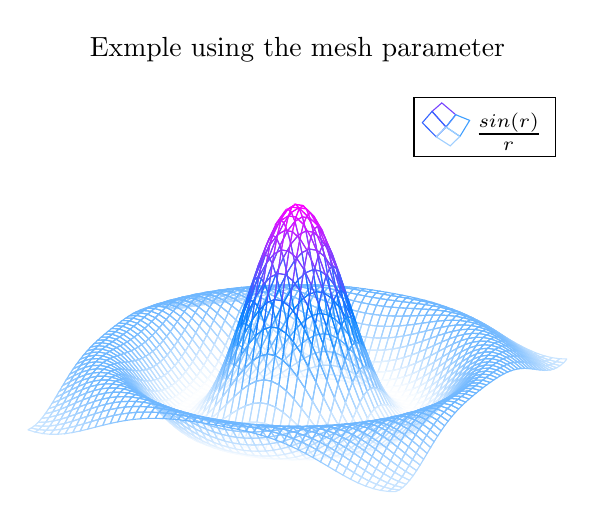
\begin{tikzpicture}
    \begin{axis}[
      title=Exmple using the mesh parameter,
      hide axis,
      colormap/cool,
      ]
      \addplot3[ mesh, samples=50, domain=-8:8, ]
      {sin(deg(sqrt(x^2+y^2)))/sqrt(x^2+y^2)};
      \addlegendentry{$\frac{sin(r)}{r}$}
      \end{axis}
  \end{tikzpicture}  
  \caption{pgfplots 3D}
  \label{fig:pgfplots-3d}
\end{figure}

Besides \textit{pgfplotstable} and \textit{pgfplots}, we could
aslo use \textit{tgiz} package or \textit{circuitkiz} to
\verb|\draw| pictures from within your LaTeX document.

\section{center and centering}
\label{sec:center-centering}

The main difference between \textit{center} environment and
\textit{centering} command is the former leave vertical space
before and after it while the later would not.

We usually use \verb|\centering{}| command within a group by curly
braces, figure, table, or
\verb|\begingroup \centering ... \endgroup|
\ref{lst:centering-within-braces}.

\begin{minipage}{1.0\linewidth}
\begin{lstlisting}[language=TeX,caption={centering within braces},label={lst:centering-within-braces}]
{\centering{centering require line break by \par, emtpy line or \\
before closing the group, otherwise text following the group wound
be centered either.}\\
}
\end{lstlisting}  
\end{minipage}

{\centering{centering require line break by \verb|\par|, emtpy
    line or \verb|\\| before closing the group, otherwise text
    following the group wound be centered either.}

} This line is not centered! Check
\href{https://tex.stackexchange.com/a/23653}{When should we use
  \texttt{\textbackslash{}begin\{center\}} instead of
  \texttt{\textbackslash{}centering}?} and
\href{http://texblog.net/latex-archive/floats/center-centering/}{center
  vs. centering}

\section{Math Equations}
\label{sec:math-equations}

To insert simple inline equation, we wrap it by \$ like
\verb|$c^2=a^2+b^2$|: $c^2=a^2+b^2$.

For tall or deep inline math expressions or sub expressions, we
can enclose them by \verb|\smash| command. This makes \LaTeX{}
ignore the height of these expressions. This keeps the line
spacing even like: \smash{$d_{e_{e_p}}$} followed by
\smash{$h^{i^{g^h}}$}.

This is an example without \verb|\smash|. You will find line space
is much bigger. A $d_{e_{e_p}}$ expression followed by a
$h^{i^{g^h}}$ one.

If we want equaton occupy a whole line, then wrap it by double
\$\$ or single bracket \verb|\[\]|. The equation will be centered
automatically.

\begin{lstlisting}[language=TeX,caption={Equation in new line},label={lst:equation-in-new-line}]
$$(1+x)^n=\sum_{k=0}^n\binom{n}{k}x^k$$
\end{lstlisting}

This is the output:
$$(1+x)^n=\sum_{k=0}^n\binom{n}{k}x^k$$
Let's have another example:
$$A_1+A_{100}$$

After examing the example above, you are recommended to tune
AUCTeX \ref{sec:auctex} configuration a little bit. Enable math
mode manually by \verb|C-c ~| or globally into Emacs startup:

\begin{lstlisting}[language=Lisp,caption={\LaTeX{} Math Mode},label={lst:latex-math-mode}]
(add-hook 'LaTeX-mode-hook 'LaTeX-math-mode)
\end{lstlisting}

We just prepend \verb|`| and type your desired math symbol. AUCTeX
automatically completes it. If given a prefix argument \verb|C-u|,
the symbol will be surrounded by dollar signs. For example, if you
type \verb|C-u ` b|, AUCTex will typeset \verb|$\beta$|. Read
AUCTex manual
\href{https://www.gnu.org/software/auctex/manual/auctex/Mathematics.html}{Entering
  Mathematics} for more details.

The \$ method by \TeX{} does provide some basic mathematics
features, but it is limited. we should
\verb|\usepackage{amsmath}|. What is more, we can
\verb|\usepackage{amssymb}| to make math symbols look shiny.

A bit further, we usually want to label and number a equation so
that we can refer to it somewhere else. Futhermore, it is better
for a long equation to occupy a new line. To do this, enclose
equation with \textit{equation} environment like
\eqref{eq:einstein}. Einstein says

\begin{equation}
  \label{eq:einstein}
  E = mc^2
\end{equation}

In order that multiple equations align properly at
\textit{ampersand \&}, we use \textit{align} or \textit{align*}
instead.  \eqref{eq:eq-alignment}. Each single equation must be
separated by \textit{linebreak \\\\}. The version with asterisk
just removes equation numbers.

\begin{align}
  \label{eq:multi-eqs}
  E &= mc^2 \\
  F &= ma
\end{align}

We use \textit{aligned} environment to align induction or
substitution lines of a single equation. Also, \textit{aligned}
should be enclosed within an equation environment.

\[
  \begin{aligned}[t]
    \label{eq:eq-alignment}
    f(x) &= x^2 \\
    \frac{1}{x} &= g(x) \\
    F(x) &= \int^a_b \frac{1}{\sqrt[3]{x}}
  \end{aligned}
\]

Compared to \textit{aligned}, \textit{align} and \textit{align*}
introduce extra space between lines to make the output
cleaner. Therefore, irrespective of single equation or multiple
equations, we'd better use \textit{align} and/or\textit{align*}.

\textit{matrix} environment must be enclosed by equation marker \&
or \textit{equatioin} environment.

\begin{lstlisting}[language=TeX,caption={Matrix},label={lst:matrix-marker}]
$
\begin{matrix}
  1 & 0 \\
  0 & 1
\end{matrix}
$
\end{lstlisting}

Similary, matrix breaks line by \verb|\\| and \& separates
columns. Here is a \textit{bmatrix} example:

\begin{equation}
  \label{eq:nn-matrix}
  A_{m,n} =
  \begin{bmatrix}
    a_{1,1} & a_{1,2} & \cdots & a_{1,n} \\
    a_{2,1} & a_{2,2} & \cdots & a_{2,n} \\
    \vdots & \vdots & \ddots & \vdots \\
    a_{n,1} & a_{n,2} & \cdots & a_{n,n}
  \end{bmatrix}  
\end{equation}

Recall that \$\$ or \verb|\[\]| let an equation placed on a new
line without label. They are equivalent to the
\verb|\begin{equation*}| environment.

\section{Document Structure}
\label{sec:file-structure}

\section{Boxes}
\label{sec:boxes}

Everything in \LaTeX{} is embedded in boxes, from letter to words,
\textit{tabular} to \textit{includegraphics}. TeX builds pages by
gluing \footnote{Squeeze and/or Stretch} boxes together according
to the default \TeX{} rules, default \LaTeX{} rules, or document
commands.

\href{https://en.wikibooks.org/wiki/LaTeX/Boxes}{Box} is of
paramount importance to get the base of \LaTeX{} typestting. Boxes
are placed relative to other boxes, while visible elements are
placed relative to the boxes which contain them.

Let's have a look at letter box illustration \ref{fig:letter-box}.

\begin{figure}[!htbp]
  \centering
  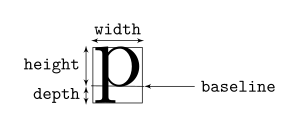
\includegraphics[width=.5\textwidth]{letter_box}
  \caption{Letter Box}
  \label{fig:letter-box}
\end{figure}

\verb|\parbox| is a box to wrap text into lines and lines are
broken into pages.

\begin{lstlisting}[language=TeX,caption={parbox box},label={lst:parbox-box}]
\parbox[pos][height][contentpos]{width}{text}
\end{lstlisting}

\textit{width} is a forced parameter to define box
width\footnote{It is \textbf{not} text width.} This argument can
be relative value like \verb|.8\textwidth|, absolute value like
\verb|5ex|, or \LaTeX{} and \TeX{} macros like
\verb|\width|. Similarly, we set \textit{height} in the same way.

\textit{pos} selects which \textit{baseline} of text to align with
neighbouring box. It can be \textbf{c}enter, \textbf{t}op, and
\textbf{b}ottom. For details, read the link above. Check
\ref{fig:parbox-baseline-alignment} for real effect.

\begin{figure}[!htbp]
  \centering
  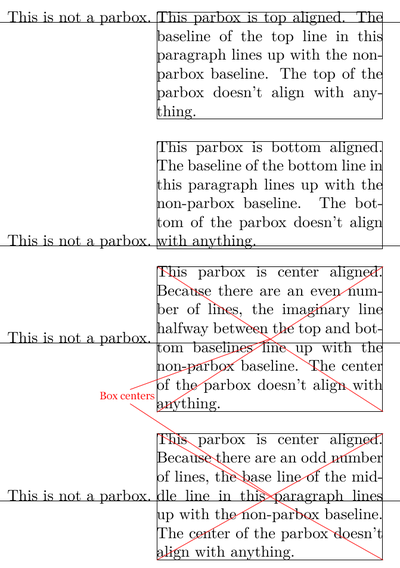
\includegraphics{parbox_baseline_alignment}
  \caption{parbox baseline alignment}
  \label{fig:parbox-baseline-alignment}
\end{figure}

This is a text line before \textit{parbox}
\parbox[t][2cm][t]{5cm}{This a text within \textit{parbox}. Please
  check text box and text alignment carefully.} This a tex line
after \textit{parbox}.

\textit{contentpos} positions the contents of the box within the
box which is straightforward. It only takes effect when box is
larger than texts it encases.

However, if the \textit{contentpos} is present and not the same as
\textit{pos} and \textit{pos} is not \textbf{c}enter, the
\verb|\parbox| will align at its borders instead of text baseline
\ref{fig:parbox-border-alignment}.

\begin{figure}[!htbp]
  \centering
  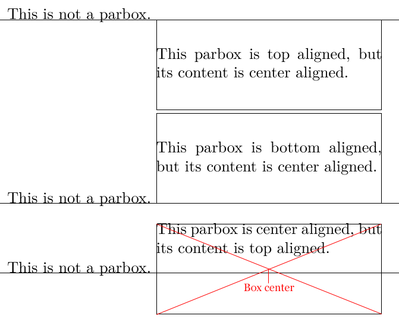
\includegraphics{parbox_border_alignment}
  \caption{parbox border alignment}
  \label{fig:parbox-border-alignment}
\end{figure}

This is a text line before \textit{parbox}
\parbox[t][2cm][b]{5cm}{This a text within \textit{parbox}. Please
  check text box and text alignment carefully.} This a tex line
after \textit{parbox}.

We also have \textit{minipage} environment box which is almost
identical to \verb|\parbox|. The difference between a
\textit{minipage} and a \verb|\parbox| is that you cannot use all
commands and environments inside a \verb|\parbox|, while almost
anything is possible in a \textit{minipage}. Hence, without
special requirement, we use the later one.

\begin{lstlisting}[language=TeX,caption={minipage box},label={lst:minipage-box}]
\begin{minipage}[pos][height][contentpos]{width} text \end{minipage}
\end{lstlisting}

Additionally, there are \textit{mbox}, \textit{makebox} and
\textit{framebox}.

In order to let multiple boxes stand side by side, we should make
sure their \textit{width} in total is less than 1, like
\ref{lst:enumerate-ordered-list}.

\subsection{input and include}
\label{sec:input-include}

Like other programming language, \LaTeX{} supports splitting large
document into different parts and
\href{https://tex.stackexchange.com/a/250}{importing} them
individually.

Use \verb|\include{filename}| in the \textit{document body} to
insert the contents of another file named
\textit{filename.tex}. Note that \LaTeX{} will start a new page
before processing the material input from
\textit{filename.tex}. \textit{include} is commonly used for
\textit{chapter} section.

\textit{include}'s sibling command
\verb|\includeonly{filename1,filename2,...}| is used in
\textit{preamble} part to insert only a subset of
\textit{included} files.

Alternatively, \verb|\input{filename}| is allowed in both
\textit{preamble} and \textit{body} parts. It does not start a new
page like \textit{include} but allow recursive \textit{include}
which is impossible for \textit{include}.

No matter which you choose, please omit \LaTeX{} file extension
\textit{.tex}.

\subsection{biblatex biber}
\label{sec:biblatex-biber}

Generally speaking, \textit{biblatex} and \textit{natbib} are
packages that handle \LaTeX{} citations in \textit{.tex} source
file. However, reference entries are stored separately in external
\textit{.bib} file. Hence, we require an intermediate tool to
format \textit{.bib} into \textit{.tex} source. That's when we
meet \textit{biber} and \textit{bibtex} which are named as
\textit{biblatex backend}.

Firstly, we should use \textit{biblatex} package:
\verb|\usepackage[backend=biber]{biblatex}|
and point out the external \textit{.bib} file to import:
\verb|\addbibresource{myref.bib}| in preamble part. Do not omit
\textit{.bib} extension.

Secondly, in the end of \LaTeX{} source (but before
\verb|\end{document}|), we print all reference entries:
\verb|\printbibliography[heading=bibintotoc]|.

Then, cite as you go. Before that, we should have a look at
\href{https://www.sharelatex.com/learn/Bibliography_management_in_LaTeX#The_bibliography_file}{\textit{.tex}
format}. The bibliography files must have the standard
\textit{bibtex} syntax. Here is a reference entry:
\begin{center}
\begin{lstlisting}[caption={BibTeX entry sample}]
@article{einstein,
    author = "Albert Einstein",
    title = "{Zur Elektrodynamik bewegter K{\"o}rper}. ({German})
    [{On} the electrodynamics of moving bodies]",
    journal = "Annalen der Physik",
    volume = "322",
    number = "10",
    pages = "891--921",
    year = "1905",
    DOI = "http://dx.doi.org/10.1002/andp.19053221004",
    keywords = "physics"
}
\end{lstlisting}
\end{center}

\verb|@article| tells the reference is an article. We also have
\verb|@book|, \verb|online| etc. \textit{einstein} is the
reference label that we will \textit{cite} with: \verb|\cite{einstein}|.

\subsection{RefTeX}
\label{sec:reftex}

RefTeX has been bundled and pre-installed with Emacs since version
20.2. We just add to Emacs:
\begin{lstlisting}[language=Lisp,caption={Enable RefTeX}]
; with AUCTeX LaTeX mode
(add-hook 'LaTeX-mode-hook 'turn-on-reftex)
; with Emacs latex mode
(add-hook 'latex-mode-hook 'turn-on-reftex)
\end{lstlisting}

To make cross-reference clickable (i.e. table of contents), use
package \textit{hyperref}.

Although \verb|C-c C-m| can prompt for \verb|\cite| command, we'd
better use
\href{https://www.gnu.org/software/auctex/manual/reftex.html}{RefTeX}
instead. RefTeX wraps itself round four LaTeX macros:
\verb|\label|, \verb|\ref|, \verb|\cite|, and \verb|\index|,
making the process more intelligent.

As mentioned earlier, RefTeX binding \verb|C-c =| displays document layout
in a newly created buffer.

To \textit{cite}, we use \verb|C-c [| binding and press \verb|^M|
\footnote{It is Enter key or Ctrl and letter `m', not Emacs Meta Alt
key.}. Afterwards, type a \textit{regular expression} to search
reference entries in \textit{.bib} file. Please be noted, there is
no completion prompt for \textit{regular expression}.

For reference to objects (i.e. figures) within the document, we
use \verb|C-c )|. For details, please visit
\href{https://www.gnu.org/software/auctex/manual/reftex/RefTeX-in-a-Nutshell.html}{RefTeX
  in a Nutshell}. RefTeX seems not to support \textit{href} to
URLs.

Sometimes, RefTeX cannot find newly created labels, references
etc. We should tell it to \textit{reftex-parse-all} or
\textit{reftex-parse-one} to parse \LaTeX{} source files.

%%% Local Variables:
%%% mode: latex
%%% TeX-master: "main"
%%% End:


\part{Mathematics}
\chapter{Combinatorics}
\label{cha:combinatorics}

Combinatorics, namely \textit{Combinatorial Mathematics}, mainly studies
\textit{permutation} and \textit{combination} of a \textit{set} or \textit{multiset}.

组合数学里经常要用到\textbf{映射}的概念,在后文的描述里,会多次出
现\textbf{对应}这样的字眼,表示两个集合间元素的映射。通常为了方便
分析,把元素、对象的不同用\textbf{编号}、\textbf{颜色}等标签来表示。

\section{Set and Multiset}
\label{sec:set-multiset}

组合数学问题总要对某个集合的元素进行操作,虽然我们通常不需要特别说明。
如~10~个人进行全排列,那么对应的集合由这~10~个人组成。

普通集合如:
\[ S = \{\, a_1,\, a_2,\, a_3,\, \dots,\, a_n\, \},\; i \in
  \mathbb{Z}: i \in [1, n] \]
表示有~$n$~种\textbf{不同}元素,并且每种元素只有一个,
称~$S$~为\textbf{单重集(合)}。

更一般的,\textbf{多重集(合)}:
\[ M = \{\; n_1 \cdot a_1,\; n_2 \cdot a_2,\; \dots,\; n_k \cdot a_k\; \} \]
突出元素\textbf{种类},即~$a_i$~表示第~$i$~种元素,而~$n_i$~则表
示第~$i$~种元素的个数。通常元素总个数用~$n$~表示:
\[ n = n_1\, +\, n_2\, +\, \dots\, +\, n_k \]
不难发现,单重集是多重集的特例,
此时
\[ k = n,\, n_i = 1,\, i \in \mathbb{Z}: i \in [1,k] \]
如果多重集里每种元素有无限个,则记为:
\[ M = \{\; \infty \cdot a_i,\; \infty \cdot a_2,\; \dots,\; \infty \cdot a_k\; \} \]
普通集合和普通排列组合对应,多重集合和多重排列组合对应,
这也是在正式介绍排列组合前先说下集合的定义。

排列组合里,集合元素通常都具体化为\textbf{不同}颜色小球,组合表示从
集合里取小球出来,而排列表示进一步把取出的小球排队,或放
进\textbf{不同}的盒子里,此时盒子的编号代表队列从头至尾的位置号。

注意符号表示的不同。单重集里~$n$~既表示元素种类和个数。而多重集
用~$k$~表示元素种数,用~$n$~和~$n_i$~表示个数。注意符号表示的
习惯:
\[ a_i,\, n_i,\, k,\, n,\, S,\, M \]

\section{Counting Principles}
\label{sec:counting-principles}

\uline{加法原理}:设集合~$S$~可以划分成若干不相交的子集~$S_1,\, S_2,\,
\cdots,\, S_m$,~则:
\[ |S| = |S_1| + |S_2| + \cdots + |S_m| \]

\uline{乘法原理}:设集合~$S$~是序偶~$(a, b)$~的集合,其中~$a$~来自于集
合~$A$, $b$~来自于集合~$B$. $A$~中每个元素~$a$~都要与~$B$~中每个元
素~$b$~配对。则:
\[ |S| = |A| \times |B| \]

\uline{减法原理}:设集合~$A$~是全集~$U$~的子集,补集
\footnote{用~overline, bar, complement,~或~smallsetminus~命令表示。
  后者的好处是同时指明了全集和子集。}\;
$\overline{A} = U \smallsetminus A = \{\, x\, |\, x\, \in U,\; x
\notin A \,\}$,~则:
\[ |A| = |U| - |\bar{A}| \]

\uline{除法原理}:设~$S$~是有限集,被划分为~$k$~个两两不相交的部分,
每部分皆有~$m$~个元素,则:
\[ k = \frac{|S|}{m} \]

后面会发现,很多应用都以单重集的排列、组合为原子操作,再结合计数四
原则完成。

\section{Permutation of Sets}
\label{sec:permutation-sets}

定义:从~$n$~个元素的单重集合~$S$~中,取出~$r$~个元素按次序排成一列,
称为~$S$~的一个~$r$-排列,记为:
\[ P(n,r),\, P_n^r,\, A_n^r \]
注意,定义里用~$r$~表示所取元素个数。

当~$r = n$~时,~$S$~的~$n$-排列简称为~$S$~的排列或~$n$~个元素
的\uline{全排列}。

从~$n$~个元素中取~$r$~个元素的排列的典型例子是从~$n$~个\textbf{不
  同}颜色的球中,取出~$r$~个,放入~$r$~个\textbf{不同}的盒子里,每
盒~1~个,盒子编号就映射成队列位置。显然第~1~个盒子有~n~种球可选,
第~2~个盒子有~$n-1$~种球可选,……,第~$i$~个盒子有~$n - (i - 1)$~种
球可选,……,第~$r$~个盒子有~$n - (r - 1)$~个球可选。

可以得出
\[ A_n^r = n(n - 1)\cdots[n - (i - 1)]\cdots[n - (r - 1)],\quad r \leq n,\quad n,\, r \in \mathbb{Z}^+ \]

定义阶乘~factorial~:
\begin{align*}
  n! &= n\times(n - 1)\times(n - 2)\cdots2\times1 \\
  0! &= 1
\end{align*}

排列组合是没会有~0~的情况的,但为了数学定义和计算的完备性,要考
虑~0~等情况。其实负数的阶成也有定义,不过在组合数学里没意义,在此不
考虑。后面还会遇到类似形式的定义。那么:

\begin{align*}
  A_n^r &= \frac{n!}{(n - r)!}, \quad 0 \leq r \leq n \\
  A_n^0 &= 1 \\
  A_n^n &= n!
\end{align*}

排列还分为\textbf{直线排列}和\textbf{圆排列}。直线排列就是我们常说
的排列,圆排列是指把取出的元素排成一个圆形,

上面定义的是\textbf{直排列},\textbf{圆排列}定义为取出的元素排成一
个圆圈,等于是让直线排列的首尾相连接。从~$n$~个元素中取出~$r$~个构
成的圆~$r$-排列数为:
\[ A_n^r/r,\quad (1 \leq r \leq n) \]因为~1~个圆排列从任一位置断开
都是一个不同的直排列,也就是说~$r$~个直排列对应~1~个圆排列,所以要
在直排列基础上\uwave{除以}~$r$.~注意,是除不是乘。 特殊的,$n$~个元
素的全圆排列数为~$(n - 1)!$.

圆排列还有一种情况是,可以翻转圆排列,如~$n$~个不同颜色的珠子串成一
条项链。一条项链的一面是一个普通圆排列,但翻转这个项链,它的另一面
是一个新有圆排列,所以每个可翻转圆排列对应~$2$~个普通圆排列。因
此,\textbf{可翻转圆排列}数为 \[ \frac{A_n^r}{2 \cdot n} \]

\section{Combination of Sets}
\label{sec:combination-sets}

上节讨论了单重集的排列,这节讲单重集的组合。排列和组合的主要区别
是\textbf{不同}元素是否有\textbf{次序}。组合取出元素\textbf{堆}在一
起,而排列在组合的基础上对取出的元素堆进行排队或入盒。

一旦取出,便不再区分组合堆内球的不同。如果取出多个堆,堆间区别
是\uwave{球的个数:堆内无序,堆间也无序}。后面多次用到这个
原则。

从~$S$~中取~$r$~个元素而不进行排序,称为~$S$~的一个~$r$-组合,实际
就是生成一个~$S$~的~$r$~元素子集,可以看成是取出元素堆在一起,没有
顺序:\uwave{组合即组堆,也即生成子集}。

组合的对应彩色球问题是从~$n$~个色彩\textbf{不同}的小球中取出~$r$~个
(堆在一起),此时没有放入盒子的操作:只取不入。如果一定要有入盒操
作,那么所有的盒子相同,没有编号区分,此时入盒与否没有意
义。~$r$~-组合数记为

\[ C(n,r),\, C_n^r,\, \binom{n}{r} \]

很显然,一个~$r$~-组合可以生成~$r!$~个排列,所以:
\begin{align*}
  C_n^r &=  \frac{A_n^r}{r!} = \frac{n!}{(n - r)!\,r!}, \quad r,\,
          n \in \mathbb{Z}_0^{+}: r \in [0, n] \\
  C_n^r &= 0, \quad r > n \\
  C_n^0 &= 1 \\
  C_n^n &= 1 \\
  C_0^0 &= 1
\end{align*}

从上面方程中的特例可以看出,完备性定义对数学计算的意义。阶乘,排列
数,组合数的完备性定义主要考虑~$r > n$~和~$n,\, r = 0$~的情况。一般
地,我们只考虑~$0 \leq r \leq n$~的情况。对于~$r,\, n < 0$~的情况
不在排列组合的讨论范围。在其它计算领域即便碰到,也不难,只要严格按
照阶乘的定义计算即可。

由公式:
\[ A_n^r = C_n^r\, r!,\quad r,\, n \in \mathbb{Z}_0^{+}: r \in [0,
  n] \]
可以得出,除原始定义外,排列操作可看作先取组合,得到一堆元素,再对
此堆列队。可以说\textbf{排列操作暗含了组合子问题}。简而言之,1 个组
合对应~$r!$~个排列,排列数是组合数的~$r!$~倍。后面更复杂的分配分组
问题也遵循此规律。

\subsection{Combination Formulas}
\label{sec:combination-formulas}

组合数的计算非常重要,因为组合公式是一个很重要的数学工具,如多项式
的系数和组合数紧密相联。本小节着重讲组合数的几个公式。

组合数和排列数计算都化成阶乘的计算。不过,当参数很大时,计算阶乘不
是件容易的事。但从组合数的原始定义可知:取~$r$~个元素得到一个子集,
余下的就是~$n - r$~元素的补集,一一对应。也就是说,每取一个~$(n -
r)$-组合就得到一个~$r$~-组合:
\[ C_n^r = C_n^{n - r}, \quad r,\, n \in \mathbb{Z}_0^{+}: r \in [0,
  n] \]
当~$r$~很大时,$n - r$~就很小,便于计算。我们还可以想办法降级阶数,
让其变得更小:
\[ C_n^r = C_{n - 1}^r + C_{n - 1}^{r - 1} \]
由此公式可得出
\href{https://zh.wikipedia.org/zh-hans/\%E6\%9D\%A8\%E8\%BE\%89\%E4\%B8\%89\%E8\%A7\%92\%E5\%BD\%A2}{
  杨辉三角形},也称~$Pascal$~三角形。

有趣的是让~$r$~遍历~$0$~到~$n$~,可以看出所有的组合数之和就是集
合~$S$~的幂集的元素个数:
\[ \sum_{r = 0}^n\binom{n}{r} = 2^n \]
此公式可以用二项式证明:
\[ (x + y)^n = \sum_{r = 0}^nC_n^rx^ry^{n - r}
\]令~$x,\, y = 1$~即可。

更一般地,组合公式的证明\textbf{双重计数~double counting}~法:从
不同(一般 2 种)角度对集合计数。更多关于双重计数,看~
\href{https://brilliant.org/wiki/double-counting-definition/}{Double
  Counting}~和
~\href{https://www.youtube.com/watch?v=TdtFxXo2zpg}{Mod-03 Lec-17
  Double counting - Part (2) }.

如上面的组合数求和公式,左边表示利用加法原则,以了集元素个数~$r$~来
对~$S$~的幂集计数。要证明,我们以另外一个角度来计数:利用乘法
原则,针对一个元素是否加入子集来计数。~$\forall a_i,\, 1 \leq i \leq
n$~要么在某个子集里,要么不在,只有两种可能。对~$a_i$~遍历,~$a_1$~有
两种可能,~$a_2$~有两种可能,……,~$a_n$~有两种可能,所以~$S$~有~$2
\times 2 \times \cdots \times 2 = 2^n$~个子集。

\subsection{Application of Combination}
\label{sec:appl-comb}

现有~$n$~个管理员管理
某\href{https://math.stackexchange.com/q/581461}{保密装
  置}(\href{https://math.stackexchange.com/q/1316831}{Minimum
  number of locks and keys})。要求任何~$\leq r$~个管理员都打不开该
装置,至少需~$r + 1$~个。假设该装置有~$s$~把钥匙,给每个管理员分配
其中的~$t$~把。问题是已知~$n,\, r,\; r \leq
n$,~求~$s,\, t,\; t \leq s$.~并进一步给出该装置的钥匙分配方案。

设管理员集合为:
\[ M = \{\, m_1,\, m_2,\, \cdots,\, m_n\, \},\; r \leq n \]
钥匙集合为:
\[ K = \{\, k_1,\, k_2,\, \cdots,\, k_s\, \},\; t \leq s \]

先求钥匙数~$s$.~由描述知,管理员集合~$M$~的任一~$r$-组合(管理员子
集)都不能凑齐~$s$~把钥匙,可知任一~$r$-组合至少还缺 1 把钥匙。显然,
任两个~$r$-组合的钥匙不能完全相同,也即不能缺同一把钥匙,否则~$2r$~个
管理员还因缺一个把钥匙而打不开保密装置,而且这样的分配方案没有意
义。~$M$~的~$r$-组合数是~$C_n^r$.~ 所以:\[ s \geq C_n^r\]

从上分析可看出,~$M$~的所有~$r$~元素子集到~$K$~的一个单射:每个~$r$元
素子集的像是它所缺失的那把钥匙。但它不一定是满射,因为~$s \gneq
C_n^r$~时,额外的钥匙会被所有的~$r$-组合所覆盖,这样的钥匙没的原像。
其中等号成立的条件是每个~$r$-组合刚好缺一把钥匙,此时构成一个满射。

再求每个管理员分得的钥匙数~$t$.
$M$~的任一~$(r + 1)$元素子集都能打开装置,说明其中任一管理员可补齐
剩下~$r$~个管理员所缺的那把钥匙。一个管理员~$m_l$~所参与的~$(r +
1)$-组合有~$C_{n - 1}^r$~个,所以:\[ t \geq C_{n - 1}^r \]

在分析钥匙的分发方案之前,让们回顾下上面的杨辉三角形,本题已出现公
式里两个分项~$C_n^r$~和~$C_{n - 1}^r$,~只不过后者的意义稍变了。

$s$~取最小值~$C_n^r$~时,我们列出~$M$~的所有~$r$~元素子集到~$K$~的
满射:\[ f(M_i) = k_j\]
\[ \{\, M_i \mid M_i \text{ is a set of size } r,\; i = 1,\,
  \cdots,\, C_n^r\, \} \xrightarrow{ \text{缺失} } K \]
显然这样的映射有很多种,我们只需选其一,如下图所示:

\begin{center}
  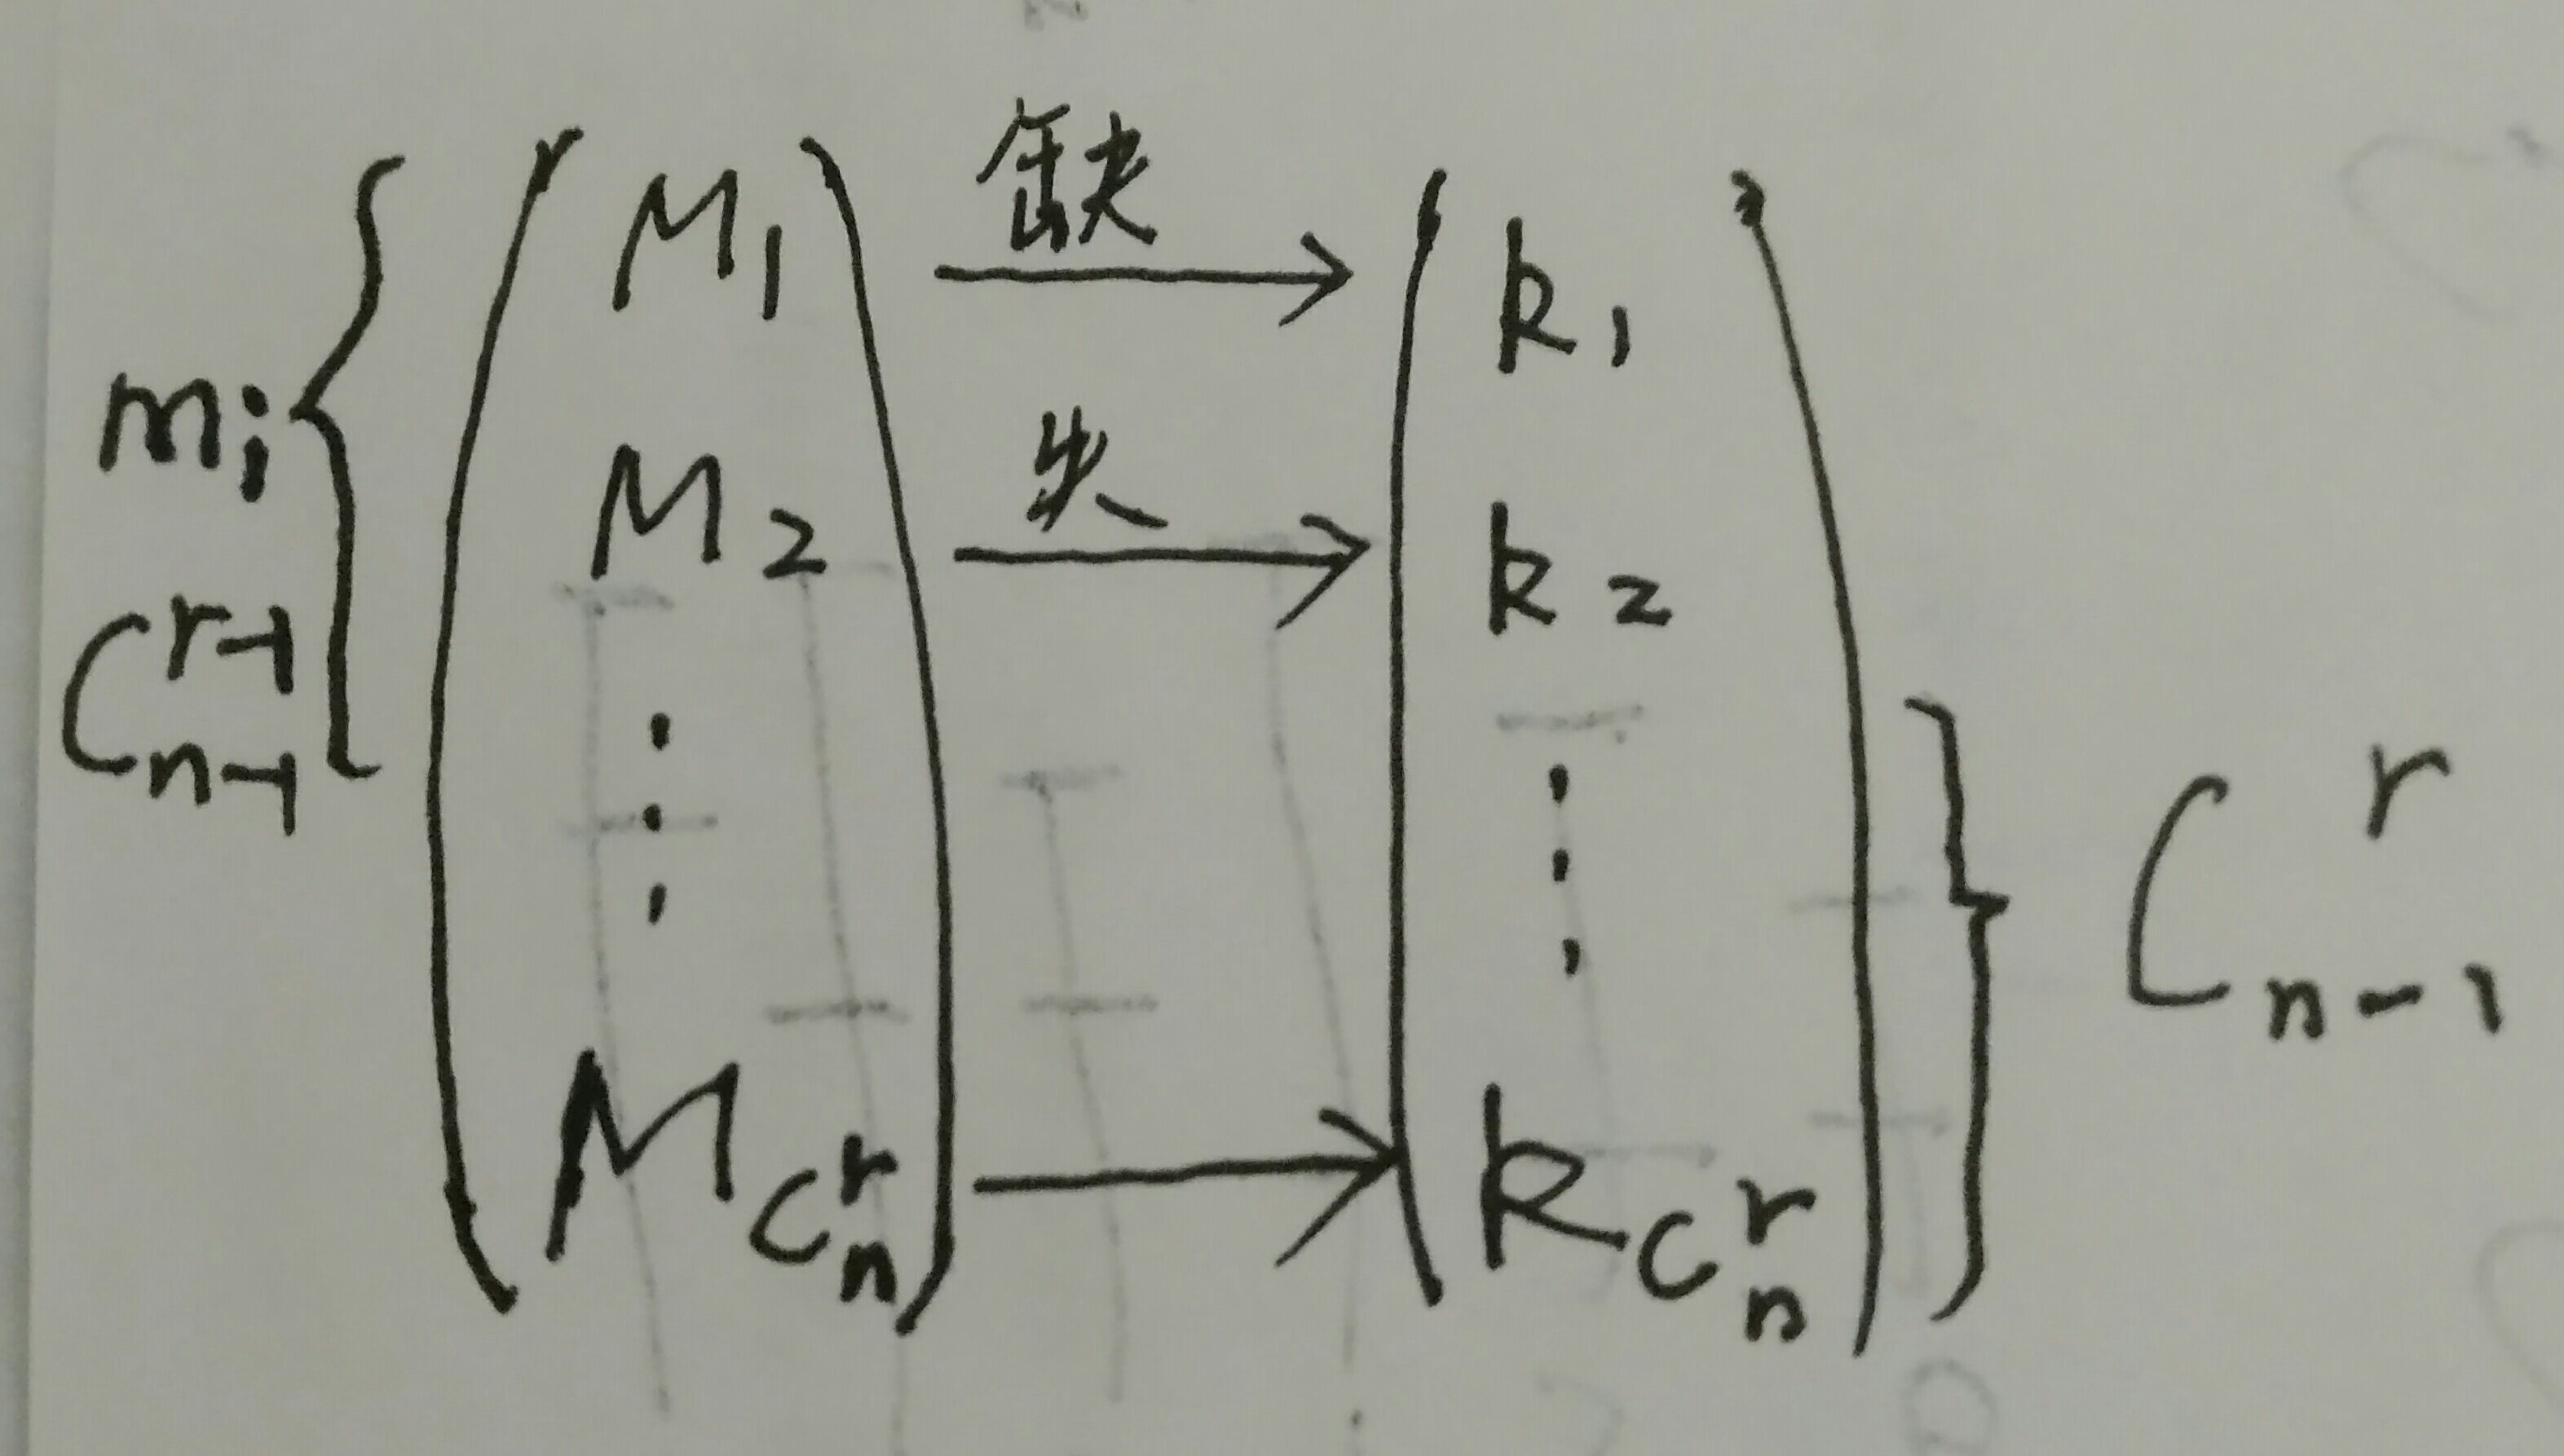
\includegraphics[width=.5\textwidth,scale=0.1]{injection}
\end{center}

对于某个管理员~$m_l$,~他所在~$r$~元素子集有~$C_{n - 1}^{r - 1}$~个,
到此,杨辉三角形公式里三个分项全部出现。很显然这管理员也缺失了这
些~$r$~元素子集对应的钥匙像,所以该管理员应分得剩下的~$C_{n -
  1}^r$~个钥匙像。针对所有管理员进行类似分配即可。

前面提过,当~$s,\, t$~的不等式不取等号时,此映射不是满射,有钥匙没有原
像,此时要求所有的~$r$~-组合都包含这样的钥匙。

现假设~$s = C_n^r + 1$,~此时的分配方案只需在原基础上稍加修改即可:
多出的这枚新钥匙再分配给每个管理员。这样~$t = C_{n - 1}^r + 1$.~此
设计仍满足保密要求。我们会发现这样的额外钥匙是没有必要的。每个管理
员都多了 1 枚同样的钥匙,起不到额外的安全作用。

分配方案的关键是根据~$s$~值列出~$r$元素子集到钥匙的
映射。现给出一个实际的例子。如果
~$n = 5,\, r = 3$,~则~$s = C_5^3 = 10,\, t = C_4^3 = 4$.~
下面给出一个映射。多出的一个钥匙(编号 11)是为了说明映射不一定是满射。

\begin{center}
  \begin{displaymath}
    \xymatrix@R=1mm{
      123 \ar[r]^{\text{缺}} & 1 \\
      124 \ar[r]            & 2 \\
      125 \ar[r]            & 3 \\
      134 \ar[r]            & 4 \\
      135 \ar[r]            & 5 \\
      145 \ar[r]            & 6 \\
      234 \ar[r]            & 7 \\
      235 \ar[r]            & 8 \\
      245 \ar[r]            & 9 \\
      345 \ar[r]            & 10 \\
                            & 11 }
  \end{displaymath}
\end{center}

每个管理员参与了~$C_{5 - 1}^{3 - 1} = 6$~个 3 元素子集,对应到映射
图上,有 6 行。不失一般性,管理员~$m_1$,~叁与了前 6 行,缺失前 6
枚钥匙,所以分得后 4 枚钥匙~$7,\, 8,\, 9,\, 10$.~依此类推,我们可
以得出如下分配方案。注意,该方案考虑到了第 11 枚钥匙。

\begin{table}[!htbp]
  \centering
  \begin{tabular}{c|*{11}c}
    \toprule
    \diagbox{Managers}{Keys} & 1 & 2 & 3 & 4 & 5 & 6 & 7 & 8 & 9 & 10 & 11 \\
    \midrule
    1 & 0 & 0 & 0 & 0 & 0 & 0 & 1 & 1 & 1 & 1 & 1 \\
    2 & 0 & 0 & 0 & 1 & 1 & 1 & 0 & 0 & 0 & 1 & 1 \\
    3 & 0 & 1 & 1 & 0 & 0 & 1 & 0 & 0 & 1 & 0 & 1 \\
    4 & 1 & 0 & 1 & 0 & 1 & 0 & 0 & 1 & 0 & 0 & 1 \\
    5 & 1 & 1 & 0 & 1 & 0 & 0 & 1 & 0 & 0 & 0 & 1 \\
    \bottomrule
  \end{tabular}
  \caption{Safe Device}
  \label{tab:safe-device}
\end{table}

\section{Permutation of Multiset}
\label{sec:permutation-multiset}

排列组合还会考虑所取元素元素是否\textbf{重复},从而生成(多)重排列
和(多)重组合。

前面两节介绍了单重集的排列组合,对应地,多重集也有排列组合,定义和
单重集一样,唯一的区别是取出的元素可能有重复。

设多重集~$M$~为:
\[ M = \{\; n_1 \cdot a_1,\; n_2 \cdot a_2,\; \dots,\;
  n_k \cdot a_k\; \},\quad \forall i = 1,\, 2,\, \cdots,\, k,\; r
  \leq n_i \]
或:
\[ M = \{\; \infty \cdot a_i,\; \infty \cdot a_2,\; \dots,\;
  \infty \cdot a_k\; \} \]
由于每种元素的个数超过所取数,所以排列里~$r$~个元素可能全部来自某
一种。

多重集~$M$~的~$r$-排列数是:\[ k^r \] 这是很容易理解的,因为队中每
个位置都有~$k$~种可能。

多重集~$r$-排列对应的彩球模型可以看成\textbf{可放回}(可重复)地对
单重集取球、排队或入盒。单重集里每个元素可无限重复使用,标记好队列
位置后又放回球堆里。当然按照多重集的定义,可以看成是对多重集取球、
排队或入盒。如不多于四位的三进制数的个数为~$3^4$.  ~对应的多重集
是
~$M = \{\, \infty \cdot 0,\, \infty \cdot 1,\, \infty \cdot 2\,
\}$.

如果~$r = n = \sum_{i = 1}^kn_i$,~则称为~$M$~的全排列。多重集全排
列(也即~$n$-排列)是对\textbf{有限集}~$M$~的\textbf{所有}元素
(如彩球)进行操作。具体来说,就是对全部~$n$个~$k$~种颜色的球进行排队。

显然此时~$r$~大于所有的~$n_i$. $M$~的全排列数为:
\[ \frac{n!}{ n_1!\, n_2!\, \cdots\, n_k! } \]

全排列的证明可以先从直觉来分析。~$n!$~表示所有元素的全排列,但
是~$a_i$~在队列重复了~$n_i$~次,这此重复实际只表示一种队列,所以除
以~$n_i!$.~如果某个~$n_i$~等于 1,~那么在被除式中是~1!.

有趣的是,实际证明中,用的是组合思路。第 1 种元素~$a_1$~要占据队列里
的~$n_1$~个位置,所以有~$C_n^{n_1}$~种可能,第二种元素要占据剩
下~$n - n_1$~个位置中的~$n_2$~个,所以有~$C_{n - n_1}^{n_2}$~种可
能,……,依此类推,最后一种元素有~$C_{n_k}^{n_k} = 1$~种可能:
\[ C_n^{n_1}\, C_{n - n_1}^{n_2}\, \cdots\, C_{n_k}^{n_k} = \frac{n!}{ n_1!\, n_2!\, \cdots\, n_k! } \]

从证明过程可知,当~$k = 2$~时,多得集的全排列数在数值上等于单重集的
组合数~$C_n^{n_1} = C_n^{n_2} = n!/(n_1!\, n_2!)$.~如用两面红旗,三
面黄旗依次悬挂在一根旗杆上,问可以组成多少种不同的标志?答案
是~$5!/(2!\, 3!) = 10$.

下面看一个棋盘的例子。在一个~$k \times k$~的棋盘上放~$k$~个车,使
得任意两个车之间不能互吃,有多少种方法?棋盘上车全是相同的,没有区
别。要想车不不互吃,任意两个车的行列值都不同。每行一个车
$a_{1\,j_1},\, a_{2\,j_2}\, \cdots\, a_{k\,j_k}$
,只需给不同行的车选列即可,所以方法数是~$k!$.

假设是~$k$~个不同(色)的车呢?保持上面排列不变,现对车的颜色进行
调换,有~$k!$~种,所以方法数是~$k! \, k!$.~实际是对车所在的行进行
全排列,也即行和列都要全排列。行的全排列负责车的不同,而列的全排列
负责车不互吃。

假设是~$n_1$~个红车,$n_2$~个蓝车,……,$n_k$~个黄车,总共~$n$~个呢?
先解决车在行上的全排列:$\frac{n!}{n_1!\, n_2!\, \cdots\, n_k!}$.
再针对不同的列全排列~$n!$.~方法数是:
\[ \frac{n!}{n_1!\, n_2!\, \cdots\, n_k!}\, \cdot\, n! \]

多重集~$r$-排列要求每种元素个数不少于~$r$,~若~$\exists t,\, n_t <
r$,~那么情问变复杂了。这时没有公式计算,要具体针对~$n_t$~列举分析。
如第~$t$~种元素出~$1,\, 2,\, \cdots,\, t$~个。

例:9 个元素的多重集~$S = {\, 3 \cdot a,\, 2 \cdot b, 4 \cdot c
  \,}$~的 8-排列数为多少?此例中,~$r = 8$~大于~$n_i$,~所以不能套
用公式。$n = 9$~只比~$r$~大 1,~所以列队中,~$a,\, b,\, c$~之一少出
一个元素。如少一个~$a$~排列数是~$\frac{8!}{2!\,2!\,4!}$,~同理可算
另两项,再用加法原则:
\[ \frac{8!}{2!\,2!\,4!} + \frac{8!}{3!\,1!\,4!} +
  \frac{8!}{3!\,2!\,3!} \]

\begin{figure}[!htbp]
  \centering
  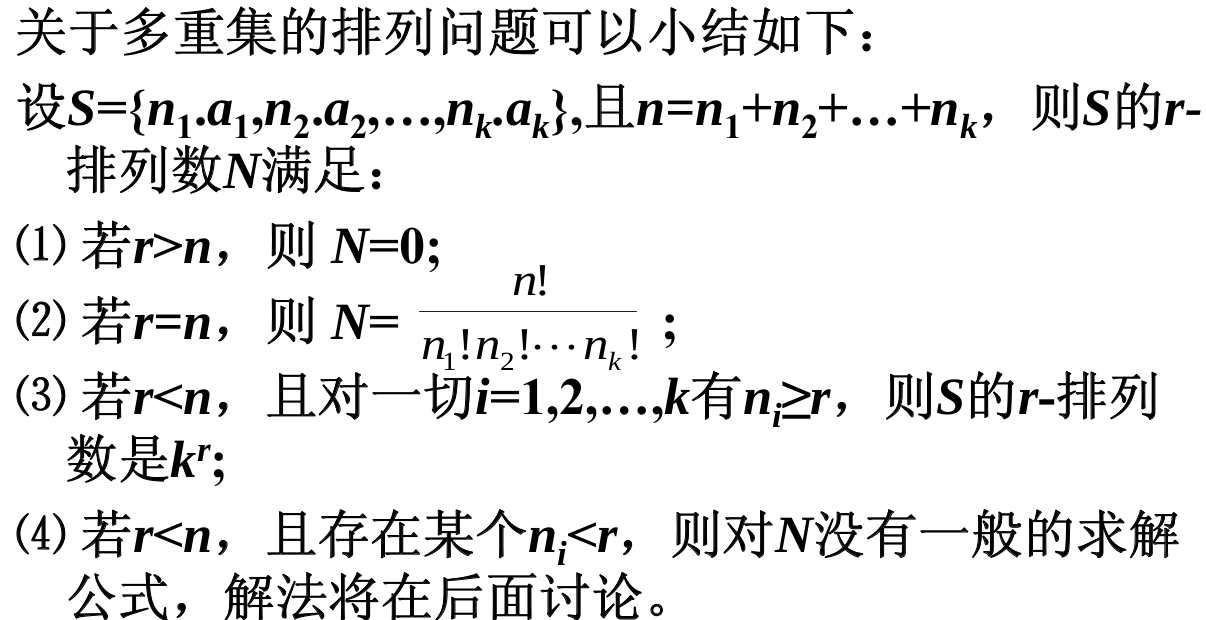
\includegraphics[width=1.0\textwidth]{SummPermMul}
  \caption{Summary on Multiset Permutation}
\end{figure}

\section{Combination of Multiset}
\label{sec:combination-multiset}

多重集~$S$~的含有~$r$~个元素的子多重集就叫做~$S$~的~$r$-组合,或表
述为取出~$r$~个元素的堆。和多重集的排列比少了列队操作。

同多重集的组合样,假设每种元素个数都不小于~$r$.~方法数即~$k$~元线
性不定方程:
\[ r = x_1\, +\, x_2\, +\, \cdots\, + x_k,\quad x_i \in
  \mathbb{Z}_0^+,\; i = 1,\, 2\, \cdots,\, k \] 的非负整数的解数。
\uwave{非负}是表明可能某~$x_t$~为 0, 此时元素~$a_t$~没有出现在组合
堆里。

计算用
\href{https://zh.wikipedia.org/zh-cn/\%E9\%9A\%94\%E6\%9D\%BF\%E6\%B3\%95}{
  隔板法}或
\href{https://zh.wikipedia.org/wiki/\%E6\%8F\%92\%E7\%A9\%BA\%E6\%B3\%95}{
  插空法}。

可以看成这样,有~$r$~个 1 在一行上,占有~$r$~位置,包含首尾共有~$r +
1$~个空位,插上~$k - 1$~个板子。第~$i$~板子前面的 1 个数是~$x_i$~的
解,第~$k - 1$~个板子后面的 1个数是~$x_k$~的解。如果某个板~$k_t$~前
没有 1 而是另一个板(两个板子处在同一空位),则~$x_t$~解为 0. 如从
\[ |\; 1\; |\; |\; 1\; 1\; \cdots\; 1\; 1\; | \] 
看出:
\[ x_1 = 0,\, x_2 = 1,\, x_3 = 0,\, x_k = 0 \]

非负正整数解的思路是:$r$~个 1 的位置和~$k - 1$~的板位置共~$r
+ (k - 1)$~个位置,从中取~$r$~个作为 1 的位置或取~$k - 1$~个作为板
的位置:
\[ C_{r + k - 1}^r \quad \text{or} \quad C_{r + k - 1}^{k - 1} \]

不考虑多重集组合,单就方程本身来说,如果是求正整数解呢?
\[ r = x_1\, +\, x_2\, +\, \cdots\, + x_k,\quad x_i \in
  \mathbb{Z}^+,\; i = 1,\, 2\, \cdots,\, k \]
正整数解暗含了~$r \geq k$,~非负解则无此限制。$r$~个 1 形中间有~$r
- 1$~个空档,插入~$k - 1$~个板,且每个空档最多一个板,则解数:
\[ C_{r - 1}^{k - 1} \]
这比非负情况的简单。

实际非负整数解和正整数解之间可以互相转换,形成一个满射,而解个数不
变。下面是把非负解转成正整数解的方法,即变量加 1:
\[ r\, +\, k =\, (x_1 + 1)\, +\, (x_2 + 1)\, +\, \cdots\, + (x_k + 1),\quad
  x_i \in \mathbb{Z}_0^+,\; i = 1,\, 2\, \cdots,\, k \]
新方程的解和原方程的解一一对应(满射:减一),这种变换思路很重要。
新方程的解是正整数解:
\[ C_{r + k - 1}^{k - 1} \]

把正整数解转成非负解,是把变量减 1.~利用转换原理,我们把方程:
\[ x_1 + x_2 + x_3 + x_4 = 20,\quad x_1 \geq 3,\, x_2 \geq 1,\,
  x_3 \geq 0,\, x_4 \geq 5 \]
转成非负解形式:
\[ (x_1 - 3) + (x_2 - 1) + (x_3 - 0) + (x_4 - 5) = 11,\quad x_1
  \geq 3,\, x_2 \geq 1,\, x_3 \geq 0,\, x_4 \geq 5 \]
或正整数解形式:
\[ (x_1 - 2) + (x_2 - 0) + [x_3 - (-1)] + (x_4 - 4) = 15,\quad x_1
  \geq 3,\, x_2 \geq 1,\, x_3 \geq 0,\, x_4 \geq 5 \]
后用插板法。

总结:

\begin{itemize}
\item 正整数:插板不相临;从中间空槽取~$k - 1$.
\item 非岁整数:插板可相监;从位数取~$k - 1$.
\end{itemize}

\section{Polynomial}
\label{sec:Polynomial}

这节谈下多项式和多重集排列、组合之间的联系。多项式:
\[ (x_1 + x_2 + \cdots + x_k)^n \]
的
\href{https://zh.wikipedia.org/zh-hans/\%E4\%BA\%8C\%E9\%A1\%B9\%E5\%BC\%8F\%E5\%AE\%9A\%E7\%90\%86#\%E5\%A4\%9A\%E9\%A1\%B9\%E5\%BC\%8F\%E5\%B1\%95\%E5\%BC\%80}{
  展开式}
可写成:
\[ \sum_{n_1 + n_2 + \cdots + n_k = n}\frac{n!}{n_1! n_2! \cdots
    n_k!}  x_1^{n_1} x_2^{n_2} \cdots x_k^{n_k},\quad n_i \in
  \mathbb{Z}_0^+: n_i \in [0,n],\; i = 0,1,\cdots,k \]
由此可看出,多项式的每项的系数是一个多重集的全排列数
$\frac{n!}{n_1! n_2! \cdots n_k!}$.~还可算出展开式的项数是多重集组
合数$\binom{n + k - 1}{n}$.

如果原多项式里~$x_i$~前还带有系数如~$a_i$:
\[ (a_1x_1 + a_2x_2 + \cdots + a_kx_k)^n \]
则情展开式的系数在多重集全排列数基础上还有乘以对应的原始系数。

如果问多项式的系数之和是多少,只需给所有~$x_i$~赋值 1 即可:
\[ (a_1 + a_2 + \cdots + a_k)^n \]
对于所有~$a_i = 1$~的情况,则系数和是~$k^n$.

\section{Grouping and Distribution}
\label{sec:group-distr}

下面是先说分组和分配问题,方法数和多重集全排列数有关。

\subsection{Distribution as Injection}
\label{sec:distr-inject}

将~$n = n_1\, +\, n_2\, +\, \cdots\, +\, n_k$~个 \textbf{不同}的
球~$a_i$~(单重集)放到~$k$~个 \textbf{不同}的对应盒子~$b_i$~里(单
重集)。~$b_1$~放~$n_1$~个,~$b_2$~放~$n_2$~个,……,~$b_k$~放~$n_k$
个。如果~$k = n$,~它就变成单重集的全排列,此时~$n_i = 1$.~简单描
述:\uline{把~$n$~个不同色球分成~$k$~堆~$n_i$,~依次分配给不同
  盒子~$b_i$}.

此模型称为\textbf{单重集的定向分配}问题。分配强调是分给\textbf{不
  同}的盒子,而定向是说~$n_i$~映射到~$b_i$,~每个盒子所分得
的\textbf{数量固定},\uline{即每堆的球数已经限定}。入盒操作相当于组
球堆贴标签。

计算过程和多重集全排列的类似,选取~$n_1$~个~$C_n^{n_1}$,~再在剩下
球里取~$n_2$~个~$C_{n - n_1}^{n_2}$, ……

这个取堆顺序是~$n_1,\, n_2,\, \cdots,\, n_k$,~实际按~$i$~的任何一
种排列顺序来取都可以,只要所取之堆放入对应的盒子子即可。如第一次
取~$n_5$个,~相当于给盒子~$b_5$~取球,那么取出后就放入盒子~$b_5$.

计算如下:
\[ C_n^{n_1}\,C_{n - n_1}^{n_2}\,\cdots\,C_{n_k}^{n_k} = \frac{n!}{ n_1!\, n_2!\, \cdots\, n_k! } \]
此计算利用了\uwave{乘法原则}。

最后,多重集全排列计算过程是给每种色球找队列位置(共~$n$~个),而上
面的模型是给每个盒子(共~$k$~个)选色球。此模型里彩球集合和空盒集合
是单重集,但放球后,盒子集合是多重集。每个盒子代表一种元素,里面的
球数代表这种元素的个数。

\subsection{Grouping}
\label{sec:grouping}

定向分配把球堆分给不同但固定的盒子,如取球放入~$k$~个的相同的盒子里
(盒子没有编号),此模型称为 \textbf{单重集的分组}问题。

由于盒子相同,所以有没有入盒操作对结果不影响,所以入盒是一个空操作。
所以有的题里,只提到分组,没有入盒操作(如分派给谁)。单重集分组可
以看成把取出球堆也堆在一起,形成一个大堆,大堆内元素是小球
堆:\uwave{分组即分堆}。

不失一般性,假设按~$n_1,\, n_2,\, \cdots,\, n_k$~的顺序取堆,如果
就此打住,那就成了定向分配。到底区别哪?没有\textbf{去重}!

球堆的区别是球个数~$n_i$~值的大小(球已取完,不再考虑其不同),可
能\uwave{某些堆的球数相等},这些堆算作是相同的堆。

不失一般性,假设~$n_1 = n_2 = n_3$~这 3 个堆球数相等,它们之间先取
谁后取谁没有变化,同理~$n_7 = n_9$~这 2 个堆的先后也不改变分组操作(没
有特殊说明,后面都据此假设)。所以要除掉重复:
\[ \frac{C_n^{n_1}\, C_{n - n_1}^{n_2}\, \cdots\, C_{n_k}^{n_k} }{
    3! \, 2! } \]
对所有的相同数值做类似去重除法即可。做题时,尽量把相同的~$n_i$~写
在一起,好去识别重复。

我们有理由把
\[ \{ n_1, n_2, \cdots, n_k \} \]
看成多重集:这~$k$~个值分成~$l$~种,每种里有~$t_j,\; j = 1, 2,
\cdots, l$~个元素,有~$\sum_{j = 1}^lt_j = k$.~拿上面的例子来说:
\[ \{ 3 \cdot n_1,\; 1 \cdot n_4,\; 1 \cdot n_5,\; 1 \cdot n_6,\;
  2 \cdot n_7,\; \cdots,\; 1 \cdot n_k \} \]
所以去重就是除以多重集每种元素个数的阶乘
~$t_1! \, t_2! \, \cdots \, t_j!$,~所以标准表达是:
\[ \frac{C_n^{n_1}\, C_{n - n_1}^{n_2}\, \cdots\, C_{n_k}^{n_k}
  }{t_1! \, t_2! \, \cdots \, t_j! } \]

一个特例是,所有~$n_i$~全相等,表示是\uline{平均分组},所以:
\[ \frac{C_n^{n_1}\, C_{n - n_1}^{n_2}\, \cdots\, C_{n_k}^{n_k} }{
    k! } = \frac{ n! }{ k! \, [ (\frac{ n }{ k })! ]^k } \]

再回过头看定向分配,发现可以分解成分组、定向分配 2 步:
\[ \frac{C_n^{n_1}\, C_{n - n_1}^{n_2}\, \cdots\, C_{n_k}^{n_k} }{
    3! \, 2! } \cdot\, 3! \, 2! \]
先把不同球数的堆放入对应的盒子。后面乘以~$3!$~表示~$n_1 = n_2 =
n_3$~这 3 个堆和~$b_1, b_2, b_3$~间可任意分派。乘以~$2!$~也是同
样的道理。

一句话:\textbf{分配问题暗含了分组子问题}。

\subsection{Distribution without Injection}
\label{sec:distr-with-inject}

有定向就有不定向,不定向分配也把球堆分派给不同的盒子,但是没有固定
分配关系:球堆~$n_i$~和盒子~$b_j$~间没有固定映射关
系。\uline{把~$n$~个不同色球分成~$k$~堆~$n_i$,~分配给不同盒
  子~$b_j$}.~此模型称为 \textbf{单重集的不定向分配}问题。

始终记住,盒子的不同、盒子编号代表队列位置。不定向分配分解成分组、
不定向分派 2 步:
\[ \frac{C_n^{n_1}\, C_{n - n_1}^{n_2}\, \cdots\, C_{n_k}^{n_k} }{
    3! \, 2! } \cdot\, k! \]
由于分组里已考虑到重复问题,后面的排列就不再考虑~$3! \, 2!$~重复,
而应把~$n_1 = n_2 = n_3$~看作是不同的堆,否则就会多次去重。

不定向分配还可以看成在定向分配基础上对~$k$~个球堆(数值~$n_i$)进行
全排列操作,方法数是:
\[ C_n^{n_1}\, C_{n - n_1}^{n_2}\, \cdots\, C_{n_k}^{n_k}\, \cdot
  \text{球堆全排队数} \]

在前节分组问题说到,堆的球数~$n_i$~是个多重集,所以我们乘以多
重集的全排列数:
\[
  \begin{aligned}[t]
    C_n^{n_1}\, C_{n - n_1}^{n_2}\, \cdots\, C_{n_k}^{n_k}\, \cdot
    \frac{ k! }{ 3! \, 2!}
    &= \frac{C_n^{n_1}\, C_{n - n_1}^{n_2}\, \cdots\, C_{n_k}^{n_k} }{
      3! \, 2! } \cdot\, k! \\
    &= \frac{n!}{ 3!\, 2!\, \cdot\, n_1!\, n_2!\, \cdots\, n_k! }\, \cdot\, k!
  \end{aligned}
\]
公式的推导过程也说明了不同的解题思路。

计算过程总结:

\begin{minipage}{1.0\linewidth}
  \begin{enumerate}
  \item 球一旦取出,组合计数完毕,就不再考虑球的不同。
  \item 取出的球堆区别于堆内球的个数。
  \item 可能某些堆球数相等,这些球堆看作是相同的堆。其实是一个多重
    集。
  \end{enumerate}
\end{minipage}

\subsection{Distribution of Multiset}
\label{sec:distr-mult}

上面的问题里,单重集每个球不同,如果所有球全相同呢?若像单重集分组
分配样规定~$n_i$,~则堆数确定,分组问题固定,只有 1 种方法。定向分
配问题:~$n$~个相同的球分成~$k$~组~$n_i$~定向派给不同盒子~$b_i$,~
也只有 1 种方法。不定向分配数是多重集的全排列如~$\frac{ k! }{ 3!
  \, 2! }$.

所以一般不规定堆内球数,如把~$n$~个同色球放入~$k$~个不同的盒子
里,盒子不为空。其实这个问题可化成求~$k$~元线性不定方程的正整数解。
方法数是:
\[ C_{n - 1}^{k - 1}\]

此时小球可看作是只有 1 种元素的多重集~$M = \{\, n \cdot a_1\, \}$.
此模型可称为含 1 种元素的\textbf{多重集定向分配}问题。

如果盒子可以为空,则化成求方程的非负整数解。

含一种元素的\textbf{多重集分组和不定向分配}问题没有统一解法,因为分
组和不定向要考虑去重问题,但是去重的前担是要知道~$n_i$~数值。所以只
能一一列举出方程解,再考虑每种解的去重,无法直接写出计数公式。

\section{Summary}

分组分配总结:

\begin{minipage}{1.0\linewidth}
  \begin{enumerate}
  \item 单重集分组:固序取堆、去~$n_i$~重。
  \item 单重集定向分配:固序取堆。
  \item 单重集不定向分配:固序取堆、去~$n_i$~重、排列。
  \item 多重集定向分配:插板法、解方程。
  \item 多重集分组和不定向分配:没有公式,只可一一列举。
  \end{enumerate}
\end{minipage}

% http://res.tongyi.com/resources/old_article/student/5869.html 加

\chapter{卡特兰数}
\label{cha:catalan-number}

\section{卡特兰公式}

\href{https://zh.wikipedia.org/zh-hans/\%E5\%8D\%A1\%E5\%A1\%94\%E5\%85\%B0\%E6\%95\%B0}{
  卡特兰数 Catalan Number} 在许多算法计数问题中都有应用,如出栈计数,
二叉树形态计数等。卡特兰数也叫明安图数。因为最提出这数的是中国明代
数学家明安图。但因为近代以来,科学技术主要由西方科学家发起,所以很
多发现用西方人物命名。

明安图数其实是一个组合数:

\[
  \begin{aligned}
    C_n = \frac{C_{2n}^n}{n+1} = \frac{1}{n+1} \binom{2n}{n} = \frac{(2n)!}{n!(n+1)!}
  \end{aligned}
\]

卡特兰数 $C_n$ 表示对 n 个元素的某种顺序计数。注意这里符号 $C_n$ 不
是前面的 n 个元素的组合数里的 $C_n^r$.

卡特兰数可以写成另外一种形式:

\begin{align*}
  C_n &= \frac{C_{2n}^n}{n+1} \\
      &= \frac{1}{n+1} \frac{(2n)\,!}{n\,!\, n\,!} \\
      &= \frac{1}{n(n+1)} \frac{(2n)\,!}{(n - 1)\,!\, n\,!} =
        (\frac{1}{n} - \frac{1}{n+1}) \frac{(2n)\,!}{(n - 1)\,!\,
        n\,!} \\
      &= \frac{1}{n} \frac{(2n)\,!}{(n - 1)\,!\, n\,!} - \frac{1}{n
        + 1} \frac{(2n)\,!}{(n - 1)\,!\, n\,!} =
        \frac{(2n)\,!}{n\,!\, n\,!} - \frac{(2n)\,!}{(n - 1)\,!\,
        (n + 1)\,!} \\
      &= C_{2n}^n - C_{2n}^{n + 1}
\end{align*}

请注意此化简过程用到

\[
  \frac{1}{n\,(n+1)} = \frac{1}{n} - \frac{1}{n+1}
\]

在处理组合数间题时,$\frac{1}{n-1}, \frac{1}{n}, \frac{1}{n+1}$ 经常被
用到来化简。这种倒数可以和阶成结合,组成新的组合数。

上面说的是卡特兰数结果,卡特兰数的递推关系式是:

\begin{align*}
  C_n &= \frac{C_{2n}^n}{n+1} \\
  &= \sum_{k=1}^n C_{k - 1}\,C_{n - k} \\
  &= C_0C_{n-1} + C_1C_{n-2} + \cdots + C_{n-1}C_0 \\
  &= \sum_{k=0}^{n-1} C_kC_{n-1-k}
\end{align*}

如何由这个递推关系得到结果式,要用到产生式或叫母函数 Generating
Function:

\begin{align*}
  g(x) = C_0x^0 + C_1x^1 + \cdots + C_{n-1}x^{n-1} + C_nx^n + \cdots
\end{align*}

关于如何用母函数求系数,细节请参考组合学课件,这里给出计算过程。上
面公式里,我们发现每项是子规模的乘积,所以对母函数平方:

\begin{align*}
  g^2(x) &= (C_0x^0 + C_1x^1 + \cdots + C_nx^n + \cdots)(C_0x^0 + C_1x^1 +
           \cdots + C_nx^n + \cdots) \\
         &= C_0^2x^0 + (C_0C_1 + C_1C_0)x^1 + \cdots + (C_0C_n +
           C_1C_{n-1} + \cdots + C_nC_0)x^n + \cdots \\
         &= C_1x^0 + C_2x^1 + \cdots + C_{n+1}x^n + \cdots \\
\end{align*}

对上式乘以 $x$ 得:

\begin{align*}
    x \cdot g^2(x) &= C_1x^1 + C_2x^2 + \cdots + C_nx^n + C_{n+1}x^{n+1} + \cdots
\end{align*}

对上式加 $C_0x^0 = 1$ 得:

\begin{align*}
  1 + x \cdot g^2(x) &= C_0x^0 + C_1x^1 + C_2x^2 + \cdots + C_nx^n
                       + \cdots \\
                     &= g(x) \\
  x \cdot g^2(x) - g(x) + 1 &= 0
\end{align*}

解上式得:

\begin{align*}
  g(x) = \frac{1 \pm \sqrt[2]{1-4x}}{2x}
\end{align*}

通过变换,得出母函数通项关系,去除系数 $C_k$, 进而解出母函数关
于$x$ 的表达式。$g(x)$ 是最开始的系数是由 $C_k$ 定义的,通过转换后
计算出系数,就得到 $C_k$.

根据二项式的推广:

\begin{align*}
  (x + y)^\alpha &= \sum_{k=0}^\infty \binom{\alpha}{k} x^k
                   y^{\alpha - k},\; a \in \mathbb{R} \\
  \binom{\alpha}{k} &= \frac{\alpha (\alpha - 1)\cdots(\alpha - k
                      + 1)}{k!}
\end{align*}

由此得:

\begin{align*}
  \sqrt[2]{1-4x} &= [1 + (-4x)]^{\frac{1}{2}} \\
                 &= \sum_{k=0}^\infty \binom{1/2}{k} (-4x)^k \\
                 &= 1 + \sum_{k=1}^\infty \binom{1/2}{k} (-4x)^k \\
                 &= 1 + \sum_{k=1}^\infty \frac{\frac{1}{2}\frac{-1}{2}\frac{-3}{2}\cdots\frac{3-2k}{2}}{k!} (-1)^k 2^{2k} x^k \\
                 &= 1 - \sum_{k=1}^\infty \frac{1 \,3 \cdots (2k - 3)}{k!} 2^k x^k \\
                 &= 1 - \sum_{k=1}^\infty \frac{1 (2 \cdot 1) \, 3 (2 \cdot 2) \cdots (2k - 3)[2 \cdot (k-1)]}{k!(k-1)!} \, 2x^k \\
                 &= 1 - \sum_{k=1}^\infty \frac{1 \, 2 \, 3 \, 4 \, \cdots \, (2k - 3)(2k - 2)}{k!(k-1)!} \, 2x^k \\
                 &= 1 - \sum_{k=1}^\infty \frac{[2(k - 1)]!}{k!(k-1)!} \, 2x^k
\end{align*}

结合上式得:

\begin{align*}
  g(x) &= \frac{1 \pm \sqrt[2]{1-4x}}{2x} \\
  &= \frac{1 \pm [1 - \sum_{k=1}^\infty \frac{[2(k - 1)]!}{k!(k-1)!} \, 2x^k]}{2x}
\end{align*}

考虑到定义时,系数 $C_k$ 是正数,所以正负号里选负号:

\begin{align*}
  g(x) &= \frac{1 \pm \sqrt[2]{1-4x}}{2x} \\
       &= \frac{1 \pm [1 - \sum_{k=1}^\infty \frac{[2(k -
         1)]!}{k!(k-1)!} \, 2x^k]}{2x} \\
       &= \frac{1 - [1 - \sum_{k=1}^\infty \frac{[2(k - 1)]!}{k!(k-1)!}
         \, 2x^k]}{2x} \\
       &= \sum_{k=1}^\infty \frac{[2(k - 1)]!}{k!(k-1)!} \, x^{k-1} \\
       &= \sum_{k=0}^\infty \frac{(2k)!}{k!(k+1)!} \, x^k
\end{align*}

通过系数对比,得出 $C_k = \frac{(2k)!}{k!(k+1)!} = \frac{1}{k+1}\,C_{2k}^k$.

\section{卡特兰数应用}

卡特兰数的来自于应用问题,~\ref{cha:algo-stack} 通过元素进出栈顺序
数问题,来说明公式推导过程。

长度为 $2n$ 的 Dyck Word(n 个 x 和 n 个 y 组成字符串)数;n 对括
号匹配组成合法运算式数;n 个节点组成二叉树方案数;$2n+1$ 个节点的满
二叉树数都是 $C_n$. 特别此 n 个节点的二叉树,添加 $n+1$ 个叶子节点,
形成满二叉树,个数都是 $C_n$.

二叉树前序序列和中序序列的关系。给定某二叉树前序序列或后序序列,求
中序序列的可能数,结果也是卡特兰数。相当于以前序序列或后序序列入栈,
中序序列出栈。

有 $n \times n$ 的小方格组成的正方形,要求从一个对角走到别一对角,
只能横向或竖向行走,不能回头且不能穿过对角线,问有多少种单调路径?
如从左下角往右上角行走,单调路径表示每一步只能向右或向上,即向最终
方向走。如果不考虑对角线问题,则竖向应走 n 步,横向应走 n 步,
共 $2n$ 步,方法数是$C_{2n}^n$. 若考虑对角线限制,假假沿在对角线下
方走,则说明任何时刻,右向步数不少于向上步数。肯体参考上面提到的进
出栈分析。

这些不同问题可以互相转化。如进栈、出栈,Dyck Word 里的 x 和 y, 左、
右括号都互相对应。全部用数学描述是 $2n$ 个 $\pm 1$ 串。

注意卡特兰数 $C_n$ 里有 n 表示规模,但是实际问题里,n 可能表示的是
n 对元素,而不是 n 个元素。如括号匹配里,n 对括号有 n 个左括号和 n
个右括号。

%%% Local Variables:
%%% mode: latex
%%% TeX-master: "main"
%%% End:

\part{数列}

\section{等差数列}

我们知道等差数列的前 n 项和是首项加尾项乘以项数除以 2.

\[
  \begin{aligned}
    a_1 &= a_1 \\
    &= a_0 + d \\
    a_2 &= a_1 + d = a_1 + d \\
    a_3 &= a_2 + d = a_1 + 2 \cdot d \\
    & \cdots \\
    a_n &= a_{n-1} + d \\
    &= a_1 + (n - 1) \cdot d \\
    &= a_0 + n \cdot d
  \end{aligned}
\]

这里特别提到 $a_0$. 严格来说,数列下标从 1 开始(表示第一个项),0
不属于数列下标,但有时为了计算方便,要借用 $a_0 = a_1 - d$.

等差数列,任意连续三项中,前后两项之和是中间项的 2 倍,因中间项减
等差 d 是前一项,加等差 d 是后一项。

等差数列的前 n 项和:

\[
  S_n = \frac{(a_1 + a_n) \cdot n}{2}
\]

\section{等差数列幂和}

等差数列的幂和是指等差数列前 n 项的 $t\, (t = 1,2,\cdots)$ 次幂之
和:

\[
  S_t(n) = \sum_{k = 1}^n a_k^t = a_1^t + a_2^t + \cdots + a_n^t
\]

基本思路是\uline{升维:借用~$ t + 1$~次二项展开式,得到数列相临两项
  的~$t + 1$~次幂差}。一般来说,我们关注的是平方、立方,即 $t =
1,\, 2$. 后面不加说明,假设 t 为 2, 则 $t + 1 = 3$:

\[
  \begin{aligned}
    (a + b)^3 &= a^3 + 3a^2b + 3ab^2 + b^3 \\
    a_{n+1}^3 - a_n^3 &= (a_n + d)^3 - a_n^3 \\
    &= 3d \cdot a_n^2 + 3d^2 \cdot a_n + d^3
  \end{aligned}
\]

对 n 遍历:

\[
  \begin{aligned}
    a_2^3 - a_1^3 &= 3d \cdot a_1^2 + 3d^2 \cdot a_1 + d^3 \\
    a_3^3 - a_2^3 &= 3d \cdot a_2^2 + 3d^2 \cdot a_2 + d^3 \\
    & \cdots \\
    a_{n+1}^3 - a_n^3 &= 3d \cdot a_n^2 + 3d^2 \cdot a_n + d^3
  \end{aligned}
\]

对 n 个式子求和,得出公式:

\[
  a_{n+1}^3 - a_1^3 = 3d \cdot \sum_{k = 1}^n a_k^2 + 3d^2 \cdot
  \sum_{k = 1}^n a_k + n \cdot d^3
\]

此式很明显可以直接算出平方和。但此式受限于$a_0, d$ 没法直接化简,所
以我们关键是住思路。其实等差数列前 n 项和可以看成 $t = 1$, 其前 n
项和除了首尾相法加外,还可以借助 $t + 1 = 2$ 次展开式。

下面以前 n 个自然数的平方和为例介绍求解思路($a_1 = 1,\, d = 1$)。
首先,我们有:

\[
  \begin{aligned}
    a_{n+1}^3 - a_n^3 &= (n + 1)^3 - n^3 \\
    &= 3n^2 + 3n + 1
  \end{aligned}
\]

对 n 遍历:

\[
  \begin{aligned}
    2^3 - 1^3 &= 3 \times 1^2 + 3 \times 1 + 1 \\
    3^3 - 2^3 &= 3 \times 2^2 + 3 \times 2 + 1 \\
    & \cdots \\
    n^3 - (n - 1)^3 &= 3(n - 1)^2 + 3(n - 1) + 1 \\
    (n + 1)^3 - n^3 &= 3n^2 + 3n + 1
  \end{aligned}
\]

把这 n 个式子加起来:

\[
  \begin{aligned}
    (n + 1)^3 - 1 &= 3 \cdot \sum_{k = 1}^nk^2 + 3 \cdot \sum_{k =
      1}^nk + n \\
    3 \cdot \sum_{k = 1}^nk^2 &= (n + 1)^3 - 3 \cdot \frac{(1 + n)
      \cdot n}{2} - (n + 1) \\
    \sum_{k = 1}^nk^2 &= \frac{n(n + 1)(2n + 1)}{6}
  \end{aligned}
\]

通过公式,我们发现平方和($t = 2$)与线性和($t = 1$)的关系:

\[
  \frac{\sum_{k = 1}^n k}{\sum_{k = 1}^n k^2} = \frac{2n + 1}{3}
\]

对于其它等差数列,我们用同样方法。如计算 $1^2, 4^2, 7^2, \cdots,
(3n - 2)^2$.

\section{等差数列的积和}

上面讲的是等差数列每项的 t 次幂和,如果求和时,每项不是 t 次幂,而改成相临
t 项积呢?为简便起见,这里假设 $t = 2$, 更高次幂依此类推即可。

\[
  S(n) = \sum_{k = 1}^n a_k \cdot a_{k+1} = a_1 \cdot a_2 + a_2 \cdot a_3 + \cdots + a_n \cdot
  a_{n+1}
\]

类似上面方法,思路是对乘积变换,前后间可能消除子项。具体是这样
的,\uline{升维:把二项积变换三项积}:

\[
  a_n \cdot a_{n + 1} = x \cdot a_{n - 1} a_n a_{n + 1} + y \cdot
  a_n a_{n + 1} a_{n + 2}
\]

其中 x 和 y 是特定系数,实际上 $-x = y = \frac{1}{3d}$:

\[
  \begin{aligned}
    x \cdot a_{n - 1} a_n a_{n + 1} + y \cdot a_n a_{n + 1}
    a_{n + 2}
    &= x \cdot (a_n - d) a_n a_{n + 1} + y \cdot a_n a_{n + 1}
    (a_n + 2d) \\
    &= x a_n \cdot a_n a_{n + 1} - xd \cdot a_n a_{n + 1}
    + y a_n \cdot a_n a_{n + 1} + 2yd \cdot a_n a_{n + 1} \\
    &= [(x + y)a_n + (2y - x)d] \cdot a_n a_{n + 1}
  \end{aligned}
\]

x 和 y 的值应独立于 $a_0, d$ 成立,则:

\[
  \begin{aligned}
    (x + y)a_n + 2yd - xd = 1 \\
    x + y = 0 \\
    2y - x = 1
  \end{aligned}
\]

可以算出 $-x = y = \frac{1}{3d}$:

\[
  a_n a_{n + 1} = \frac{1}{3d}( -a_{n - 1} a_n a_{n + 1} +
  a_n a_{n + 1} a_{n + 2} )
\]

对 n 遍历得:

\[
  \begin{aligned}
    a_1a_2 &= \frac{1}{3d}(-a_0a_1a_2 + a_1a_2a_3) \\
    a_2a_3 &= \frac{1}{3d}(-a_1a_2a_3 + a_2a_3a_4) \\
    & \cdots \\
    a_n \cdot a_{n + 1} &= \frac{1}{3d}( -a_{n - 1} a_n a_{n + 1} +
  a_n a_{n + 1} a_{n + 2} )
  \end{aligned}
\]

得出前等差数列的前 n 项积和:

\[
  S(n) = \sum_{k = 1}^n a_k \cdot a_{k+1} = \frac{1}{3d}(a_na_{n+1}a_{n+2} - a_0a_1a_2)
\]

不难发现,此式关键是首尾两个三项积之差。注意这里借用了 $a_0$. 下面以

\[
  S(n) = 1 \times 4 + 4 \times 7 + 7 \times 10 + \cdots + (3n -
  2)(3n - 2 + 3)
\]

为例。可推出:

\[
  \begin{aligned}
    (3n - 2)(3n - 2 + 3)
    &= \frac{1}{9}[-(3n - 2 - 3)(3n - 2)(3n -
    2 + 3) + (3n - 2)(3n - 2 + 3)(3n - 2 + 6)] \\
    &= \frac{1}{9}[-(3n - 5)(3n - 2)(3n + 1) + (3n - 2)(3n + 1)(3n + 4)]
  \end{aligned}
\]

每项被变换成加减法,可以通部分抵消,达到求和目的:

\[
  \begin{aligned}
    1 \times 4 &= \frac{1}{9}[-(-2) \times 1 \times 4 + 1 \times 4
    \times 7] \\
    4 \times 7 &= \frac{1}{9}[-1 \times 4 \times 7 + 4 \times 7
    \times 10] \\
    7 \times 10 &= \frac{1}{9}[-4 \times 7 \times 10 + 7 \times 10
    \times 13] \\
    & \cdots \\
    (3n - 2)(3n + 1) & = \frac{1}{9}[-(3n - 5)(3n - 2)(3n + 1) + (3n - 2)(3n + 1)(3n + 4)]
  \end{aligned}
\]

这里 $a_0 = 1 - 3 = -2$. 所有等式相加,得:

\[
  S(n) = \frac{1}{9}[(3n - 2)(3n + 1)(3n + 4) + 8]
\]

\section{幂和与积和的联系}

至此等差数列的幂和与积和都可得出。我们发现求幂和与积和的通用思路是
\textbf{升维}。幂和借用 $t + 1$ 次二展开式,而积和借用 $t + 1$ 项积。

其实幂和可以用积和的方式计算:

\[
  \begin{aligned}
    a_n^2 &= a_n \cdot [(a_n + d) - d] \\
    &= a_n \cdot [a_{n+1} - d] \\
    &= a_n a_{n+1} - d \cdot a_n \\
  \end{aligned}
\]

%%% Local Variables:
%%% mode: latex
%%% TeX-master: "main"
%%% End:


\part{ICT}
\label{part:ict}
\chapter{Terminologies}
\label{cha:ict-terminologies}

\section{Internet and internet}
\label{sec:internet-internet}

Capitalized \uline{Internet} (Interconnected Network) is a
\textit{global} network of networks, using the TCP/IP
\textit{protocol suite} and consisting of private, public,
academic, business, and government networks of local to global
scope. There is only one Internet in the world!

On the other hand, the lower case \uline{internet} refers to any
instance of Interconnected Networks using the same type of
protocols. An internet is may or may not connect to the Internet;
may or may not use the TCP/IP protocol suite.


%%% Local Variables:
%%% mode: latex
%%% TeX-master: "main"
%%% End:

\chapter{Operating System}
\label{cha:operating-system}

\lstset{language=bash}

\section{CRLF}
\label{sec:crlf}

This sections talks about keys (and their names) and keybord.

We have \textit{physical} keyboard with labels like 1, 2, Enter,
Delete etc. The physically pressed keys are captured by OS and
then translated \textit{integer keycodes}. Programs read the
keycodes and interpret them as appropriate \textit{logical}
keys.

We can change keycodes passed from OS to a program like switching
left Ctrl and Caps. When Caps key is pressed, the Ctrl keycode is
sent to the program.

Several logical keys have their own names. Specifically, DEL, ESC,
LFD, SPC, RET, TAB, and \textit{newline} all stand for themselves
when seen in online posts. Name \verb|C-m| (pressing the
Return key) is translated to logical RET. \verb|C-k| for
pressing Control and \verb|k| simutaneously. \verb|C-j| is
translated to LFD. Don't be fooled. Logical name \verb|DEL|
corresponds to \verb|Backspace| on keyboard, not Delete.

Then let's have a look at ancient typewriter, comprising
\textit{Carriage Return} that helps feed a new line. When a new
line is required, the carriage return pulls back the typing head
and then a new paper line is fed up. So in the old times, a new
line consists of a Carriage Return and a Line Feed.

In the PC age, the corresponding keyboard key is Enter. When it is
pressed, the logical name is ENTER, also called
(\textit{electronical}) \textit{newline}. So it is not uncommon
that the Enter key has an arraw line as depicted in
\ref{fig:enter-return-key}. The vertical line means line feed
while the horizontal arrow means carriage return.

\begin{figure}
  \centering
  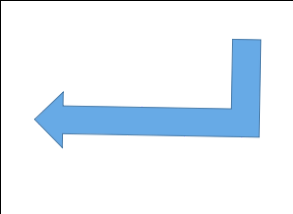
\includegraphics{return-enter-key}
  \caption{Enter/Return Key}
  \label{fig:enter-return-key}
\end{figure}

The two operations can be named as \verb|CR| and \verb|LF|
respectivelly. Programing languages, Bash included, use
\lstinline|\r| and \lstinline|\n| to denote the two names. In
Linux, it is \verb|\n|, while in Windows it is \verb|\r\n|. Mac
OS, to the contrary, is \verb|\r|. We call this \textit{line
  ending scheme}. It is critical to be aware of line ending
difference, especially when web techniques are involved like
\ref{lst:curl-crlf}.

\begin{itemize}
\item \verb|C-m, ^M, \r, Carriage Return, RET| are all the same
  thing.
\item \verb|C-j, ^J, \n, Line Feed, LFD| as well.
\end{itemize}

\section{Memory}
\label{sec:os-memory}

\subsection{Cost of Reclaiming}
\label{sec:cost-reclaiming}

The cost of memory \textit{initialization} and
\textit{destruction} of kernel data objects can actually outweigh
the cost of allocating them, which can result in significant
performance drop.

\begin{quotation}
  Kernel is reluctant to free up memory unless required.
\end{quotation}

\subsection{Slab Allocation}
\label{sec:slab-allocation}

A slab is a set of one or more \textit{continuous} memory pages
\textit{pre-allocated} for the slab allocator as an individual
\textit{cache}. This cache is further divided into \textit{equal
  segment}s (also called \textit{chunk} or \textit{slot}) in size
of the object type that the cache is managing. It is a memory
allocation mechanism intended for \textit{small} \uline{objects}
of the \textit{same type} like \textit{inode} and \textit{dentry}:

In this parlance, the word \uline{cache} or \uline{caching} refers
to a memory storage for a specific type of object, such as
\textit{semaphores}, \textit{process descriptors}, \textit{file
  objects}, etc. It is \textbf{not} the \textit{cache memory}
between the main memory and CPU.

A small object may be 8 bytes, 16 bytes, or 256 bytes large, but
usually far smaller than the size of a 4K memory page. If every
small object is allocated a separate memory page, it would be a
vast memory waste and
\href{https://stackoverflow.com/a/27762414}{lead to}
\textit{internal} and/or \textit{external} memory
\textit{fragmentation}.

\begin{landscape}
  The notion of \textit{object caching} was primarily introduced
  in order to \textit{avoid} the overhead such overheads.

  As a slab is pre-allocated, memory allocation request can be
  instantly satisfied in one of the preserved slot. Destruction of
  the object does not reclaim the slot but only puts the slot into
  the list of free slots by the slab allocator. This process
  eliminates the need to search for suitable memory space and
  greatly alleviates memory fragmentation.

  From file \lstinline|/proc/meminfo|, \uline{Slab} is the total
  amount of available slots. \uline{SReclaimable} can be freed up
  by kernel for other usage while \uline{SUnreclaim} cannot.

  For slab details, execute \lstinline|man 5 slapinfo| and
  \lstinline|slabtop|. Here is an excerpt \ref{lst:slab-info}:

\begin{lstlisting}[caption={Slab Info},label={lst:slab-info},basicstyle=\tiny\ttfamily]
# name               <active_objs> <num_objs> <objsize> <objperslab> <pagesperslab> : tunables <limit> <batchcount> <sharedfactor> : slabdata <active_slabs> <num_slabs> <sharedavail>
ext4_groupinfo_4k    364    364    144   28    1 : tunables    0    0    0 : slabdata     13     13      0
squashfs_inode_cache      0      0    640   25    4 : tunables    0    0    0 : slabdata      0      0      0
fuse_inode          3864   3864    768   21    4 : tunables    0    0    0 : slabdata    184    184      0
PINGv6                 0      0   1152   28    8 : tunables    0    0    0 : slabdata      0      0      0
RAWv6                 56     56   1152   28    8 : tunables    0    0    0 : slabdata      2      2      0
tw_sock_TCPv6          0      0    240   17    1 : tunables    0    0    0 : slabdata      0      0      0
request_sock_TCPv6      0      0    304   26    2 : tunables    0    0    0 : slabdata      0      0      0
dma-kmalloc-16         0      0     16  256    1 : tunables    0    0    0 : slabdata      0      0      0
dma-kmalloc-8          0      0      8  512    1 : tunables    0    0    0 : slabdata      0      0      0
dma-kmalloc-192        0      0    192   21    1 : tunables    0    0    0 : slabdata      0      0      0
kmalloc-8192          72     72   8192    4    8 : tunables    0    0    0 : slabdata     18     18      0
kmalloc-4096         249    272   4096    8    8 : tunables    0    0    0 : slabdata     34     34      0
kmalloc-512          864    912    512   16    2 : tunables    0    0    0 : slabdata     57     57      0
\end{lstlisting}

  The first column is the \textit{names} of different types of
  slabs. \textit{kmalloc-512} means this slab is designated for
  512-byte objects. So is \textit{dma-kmalloc-192} for 192-byte
  objects. To filter slabs larger than or equal to 10M, run:

\begin{lstlisting}
awk '{ if ( $3*$4/1024/1024 > 10 ) { print $1, $3*$4/1024/1024 } }' /proc/slabinfo
\end{lstlisting}

\end{landscape}

%%% Local Variables:
%%% mode: latex
%%% TeX-master: "main"
%%% End:

\chapter{Domain Name System}
\label{cha:domain-name-system}

\section{Contact}
\label{sec:dns-contact}

\begin{table}[!h]
  \centering
  \begin{tabular}[!h]{c}
    \toprule{}
    HU Zhan \\
    zhan.hu@chinacache.com \\
    \bottomrule
  \end{tabular}
  \caption{Contact}
\end{table}

\section{Outline}
\label{sec:dns-outline}

The system resolves a \textit{fully qualified domain name} (FQDN)
of a host to IP and mainly comprises:

\begin{itemize}
\item A distributed and decentralized \textit{database}
  implemented in a hierarchy of \textit{name servers}.
\item An application layer protocol over UDP port 53, which is
  utilized by other application layer protocols like HTTP. TCP 53
  is widely supported nowadays.
\item The name servers are often UNIX machines running the
  Berkeley Internet Name Domain (BIND) or Dnsmasq software.
\item Work in Client-Server mode.
\end{itemize}

Roles:

\begin{itemize}
\item Domain: administration sapce.
\item Domain Name: name of administration space.
\item Domain · Name Servers: implement DNS database and resolve subdomain names.
\end{itemize}

\section{Domain Tree}
\label{sec:domain-tree}

\begin{figure}[tbp]
  \centering
  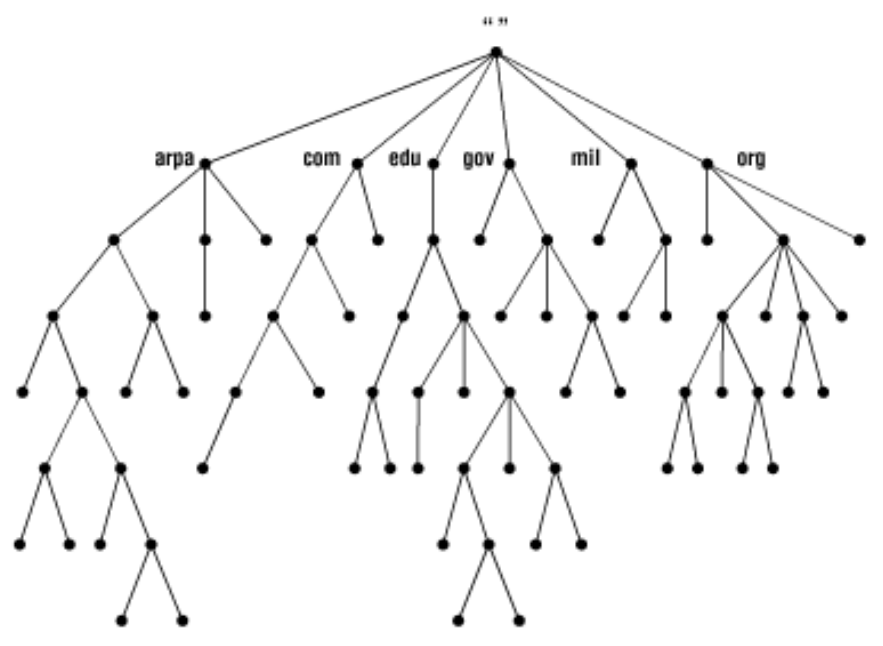
\includegraphics[scale=0.40]{domain-tree}
  \caption{Domain Tree}
  \label{fig:domain-tree}
\end{figure}

Domains define \textit{administration space} of different levels
and sizes, and can be demonstrated in a \textit{tree} structure as
depicted in figure \ref{fig:domain-tree}. External nodes
represents physical \textit{host}s. Nodes in the tree is assigned
labels, like \textit{com}, \textit{cn}, etc. A \textit{null}
\verb|""| label is reserved for the \textit{root}. But in text it
is written as a \textit{dot}. Host nodes are labelled by
\textit{hostname}s \ref{sec:dns-host}. We will find, later in the
post, each \textit{administration entity} is resposible for
managing \textit{name resolution} in its own space.

A node and the corresponding subtree represents a domain. The root
represents the whole space in DNS, namely \textit{root
  domain}. Each domain can be further divided into additional
partitions, called \textit{subdomain}s. For example, node
\textit{edu} defines a subdomain of the root domain. Domains at
the second and third layers are called \textit{Top-level Domain}
(TLD) and \textit{Authorative Domain} respectivelly.

We assign a \textit{name} to each domain, namely \textit{domain
  name}. Domain name is the sequence of labels from the
\uline{domain node} (root node of the subtree) to the
\uline{root}, with \verb|.| separating the labels. In this post,
\textit{root node} refers to that of a subtree, while
\textit{root} refers to that of the whole tree.

For instance, \textit{root domain name} is written as a dot
\uline{<.>} while \uline{<com.>} is an instance of \textit{TLD
  name}. \textit{bing.com.} is an \textit{Authorative Domain
  Name}. Attention plese; theere is one and only one root domain
name! The concepts can be illustrated as below:

\begin{quotation}
  node => subtree => domain/subdomains => domain name
\end{quotation}

DNS requires that sibling nodes have different labels to guarantee
\textit{uniquness} of domain names. Figure
\ref{fig:domain-name-uniqueness}, has two sibling nodes with
\textit{hobbes} label. That is not acceptable.

\begin{figure}
  \centering
  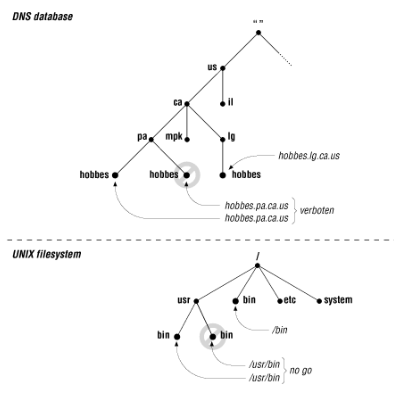
\includegraphics[scale=0.80]{domain-name-uniqueness}
  \caption{Domain Name Uniqueness}
  \label{fig:domain-name-uniqueness}
\end{figure}

The relation between domain and domain name is interesting. We can
say a domain has a domain name. We can also say a domain contains
a bunch of subdomain names. For example, a TLD named as
\textit{edu.} contains all subdomain names ending with
\textit{edu.} like \textit{berkeley.edu.} and \textit{ustc.edu.}.

Each host has domain name as well. Domain name of a host is
associated with information like IP address, name aliases, mail
routings etc. in the database. It is the original intention of DNS
to record and resolve the information associations.

Domain tree resembles the organization of an UNIX filesystem - a
database of directories and files, namely pathnames. Pathname is
analogous to domain: internal domain and directory pair, external
domain (host) and file pair are analogous. A slight difference is
the name order. In UNIX filesystem, a pathname is written in a
top-down manner while a domain name in \textit{reverse} order -
upward to the root.

\section{FQDN}
\label{sec:fqdn}

Domain name can be either \textit{absolute} or
\textit{relative}. When a domain name ends with the root label
(dot), it is an absolute domain name and also called \uline{Fully
  Qualified Domain Name} (FQDN). The root label is different from
the dot separator, though they looks the same. All domains
discussed in the prior section are absolute. Relative domain names
provided to server side will be transformed to absolute versions
by appending
\href{http://www.zytrax.com/books/dns/ch8/origin.html}{current
  ORIGIN}. The partial transformation may be done in the client
side by \textit{resolver} (check section \ref{sec:dns-resolver}).

An absolute domain name resembles an absolute pathname in UNIX
filesystem - relative to the root. A relative domain name
resembles a relative pathname - relative to the root node of a
subtree.

A relative domain name like \verb|cs.blogger| without trailing
dot, can be anywhere in the tree and may correspond to one or more
subdomains and subtrees as in figure
\ref{fig:relative-domain-name} . Analogously, multiple relative
pathnames with the same name are allowed.

\begin{figure}
  \centering
  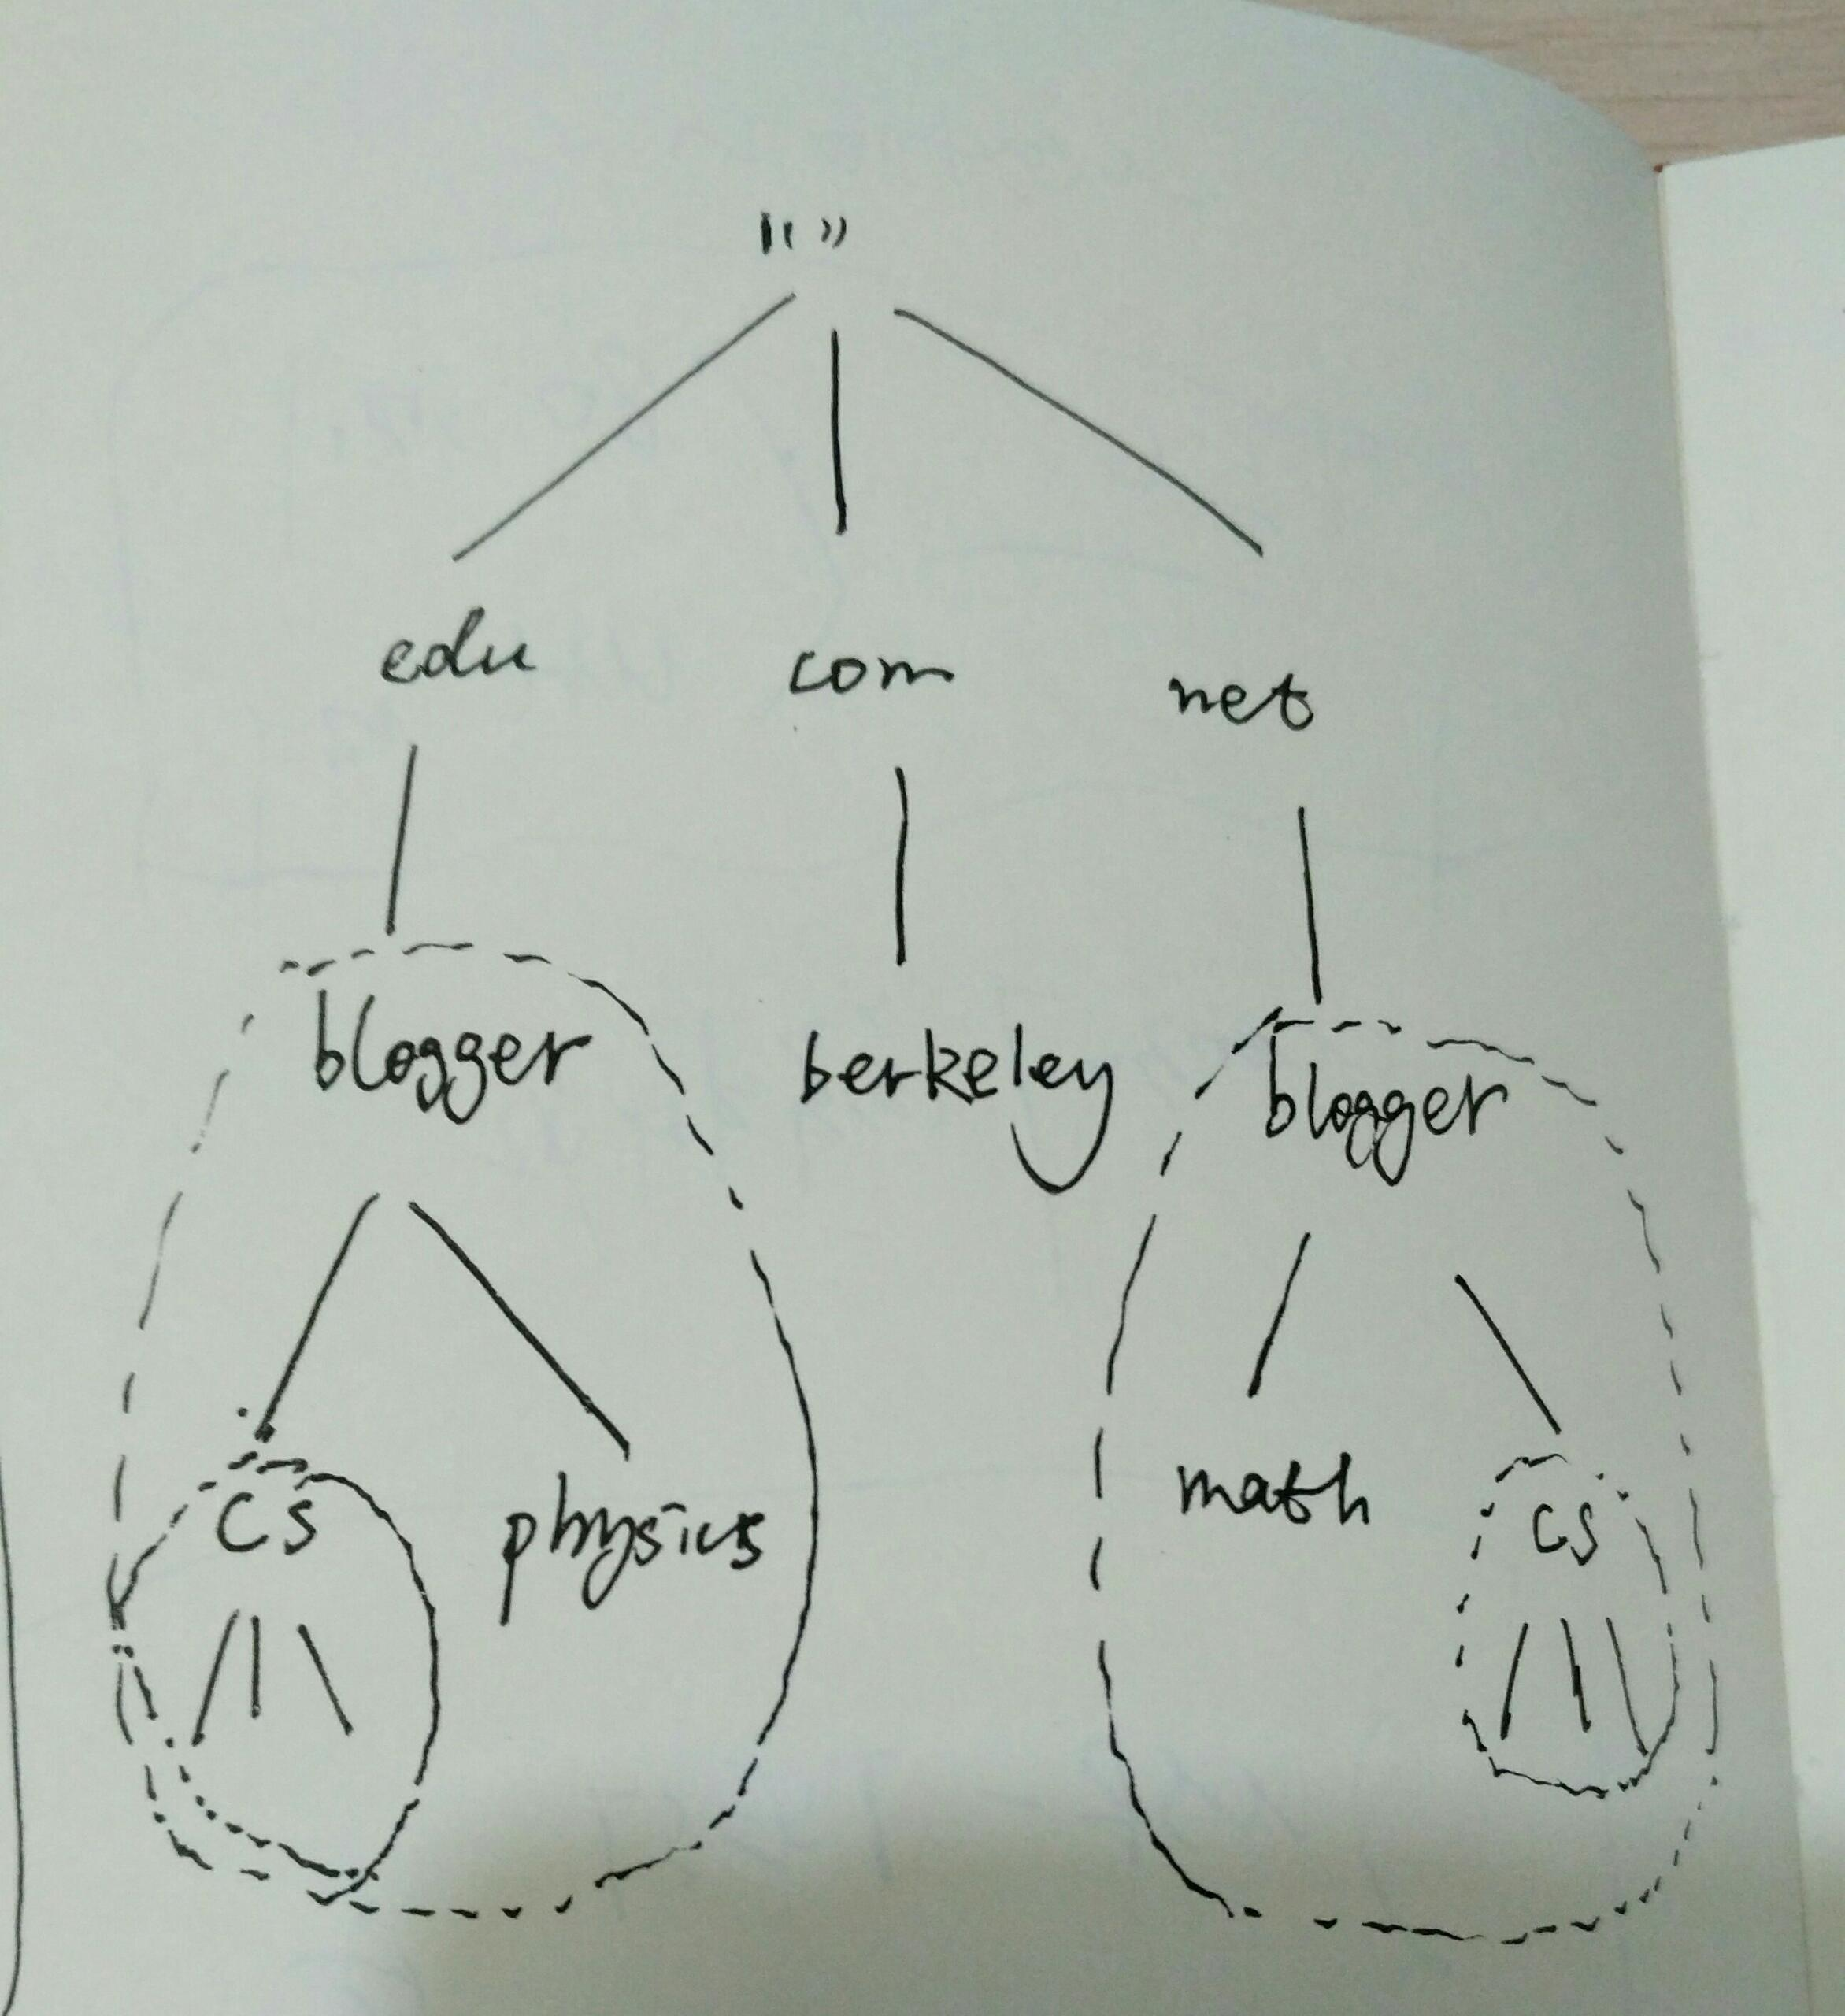
\includegraphics[scale=0.10]{relative-domain-name}
  \caption{Relative Domain Name}
  \label{fig:relative-domain-name}
\end{figure}

With respect to DNS, we'd better use FQDN as much as possible to
rid confusion.

\begin{quotation}
  Without explicit note, all domain names are \textit{absolute} in
  this post.
\end{quotation}

\section{Host}
\label{sec:dns-host}

As analyzed above, each \textit{host} has a domain name that is
also a FQDN (easy to remember by humans). Alternatively, a host
can also identified by its IP address (used by routers). FQDN of a
host can be divided into two parts, namely hostname - the first
segment, and authorative domain name - the rest part, demonstrated
in table \ref{tab:host-fqdn}:

\begin{table}[t]
  \centering
  \begin{tabular}{*{4}{|c}|}
    \hline
    www & google & com & . \\ \hline
    \multicolumn{4}{|c|}{FQDN} \\ \hline
    & \multicolumn{3}{c|}{Authorative Domain Name} \\ \hline
    && \multicolumn{2}{c|}{TLD} \\ \hline
    &&& Dot Root Domain \\ \hline
    www & google & com & . \\
    \hline
  \end{tabular}
  \caption{Host FQDN}
  \label{tab:host-fqdn}
\end{table}

\textit{hostname} in the context of DNS is different from that of
command \lstinline[language=bash]|hostname|. Instead, it is an
identfier meaningful to DNS. In the target host, both value are
not necessarily identical.

Take \textit{www.example.com.} for example, \textit{www} is the
hostname, while \textit{example.com.} is the authorative domain
name. Both names together constitute the host's FQDN.

FQDNs we use daily are actually aliases of their
\textit{canonical} versions and are far more mnemonic. A canonical
FQDN may have multiple aliases. For example,
\textit{cn-0001.cn-msedge.net.} has two aliases, one of which is
\textit{www.bing.com.}.

\begin{lstlisting}
; dig +nocookie www.bing.com cname

;; ANSWER SECTION:
www.bing.com.		60	IN	CNAME	cn.cn-0001.cn-msedge.net.
cn.cn-0001.cn-msedge.net. 36	IN	CNAME	cn-0001.cn-msedge.net.
\end{lstlisting}

About the \lstinline|dig| command, refer to section
\ref{sec:bash-dig}.

\section{Name Server}
\label{sec:domain-name-server}

How the DNS database is implemented? How domain names are
resolved? Such questions lead to the topic in this section -
\textit{domain · name server} \footnote{域 · 名字服务器}.

As mentioned in section \ref{sec:domain-tree}, an administration
entity manages domains and subdomains of its own space. An entity
can further delegates administration of subdomains to other
organizations. A domain is administrated by one and only one
entity. To the contratry, an entity can administrate one or more
domains. The core functionality of domain administration is to
implement domain · name servers and database therein,
like domain names, IPs, aliases. The entity should resolve names
of all subdomain under its coverage directly or delegate the
resolution to a sub-entity.

At the very top, we have \textit{root domain · name server}s
\footnote{根域 · 名字服务器}, then \textit{TLD · name server}s
\footnote{顶级域 · 名字服务器} at next layer, and
\textit{authorative domain · name server}s \footnote{权威域 · 名字
  服务器}. Root domain name servers are responsible to resolve TLD
names while TLD name servers are for authorative domain
names. Authorative domain name servers resolve host FQDNs instead.

\section{Resource Record}
\label{sec:resource-record}

Now let's have a closer insight into what DNS database looks
like. We call a DNS entry in the database Resource Record
(RR). The relationship line can be put like below:

\begin{quotation}
  doname name => administration space => administration entity =>
  domain name · servers =>
  database => subdomain RRs => subdomains resolution \\
\end{quotation}

RRs are indexed by domain names in DNS database. The snippet
\ref{lst:dns-database-index} are excerpts from one of the root
domain name servers. Each entry is queried by TLD name
\verb|<com.>|.

\begin{lstlisting}[caption={DNS Database Index},label={lst:dns-database-index}]
com.			172800	IN	NS	a.gtld-servers.net.
com.			172800	IN	NS	b.gtld-servers.net.
com.			172800	IN	NS	c.gtld-servers.net.
com.			172800	IN	NS	l.gtld-servers.net.
com.			172800	IN	NS	m.gtld-servers.net.
\end{lstlisting}

There exist multiple types of RRs like SOA, PTR etc. But they are
not the core of the post. Here are four common types of RRs as
follows:

\begin{itemize}
\item A: (domain name, ip)
\item NS: (domain name, domain name server)
\item CNAME: (alias, canonical domain name)
\item MX: (mail domain name, alias)
\end{itemize}

If a domain name server contains an A record for a particular
subdomain name, it is \textit{authorative} for that name. Needless
to say, it is an authorative domain name server. If a domain name
server contains an SOA record, it is also authorative (check
section \ref{sec:zone-data-file}). In this post, authorative
domain name server only refers to those resolving host FQDNs.

Most the of RRs in a name server are NS records that specify
alternative domain name servers (at a lower level \footnote{A NS
  RR reflects the delegation of administration.}) from which the
subdomain name can be resolved. It is sensible that internal FQDNs
require only NS records as they just do auxiliary jobs for
resolving external FQDNs (that of hosts).

Those alternative domain name servers, in return, are all physical
hosts in the system and should have their own external
FQDNs. Accordingly, there \textit{must} exist A records somewhere
in the system. In other words, the selected external FQDN should
be resolved first before the original query. This process may
repeat several times during the resolution course.

\section{Root Domain Name Server}
\label{sec:root-domain-name-server}

There are overall 13 root domain name servers over the world,
namely \lstinline[language=bash]|{a..m}.root-servers-net.|. The
relevant 13 IP addresses are fixed and kept by all name servers in
the system, such that there is no need to resolve root domain
name. This makes sure the resolving system starts with an initial
entrance.

Those 13 name servers are authorative for TLD names
(i.e. \uline{<com.>} and \uline{<net.>}) and contain NS records,
pointing where TLD names can be resolved. From excerpt
\ref{lst:root-ns-rr}, the root domain name server
\textit{b.root-servers.net.} contain 13 \footnote{The number of
  TLD name server is also 13.} NS records the TLD name
\textit{com.}.

\begin{minipage}{1.0\linewidth}
\begin{lstlisting}[caption={RRs in Root Name Server},label={lst:root-ns-rr},basicstyle=\tiny\ttfamily]
; <<>> DiG 9.11.2-P1 <<>> +trace www.bing.com
;; global options: +cmd
.			82248	IN	NS	d.root-servers.net.
.			82248	IN	NS	k.root-servers.net.
.			82248	IN	NS	c.root-servers.net.
.			82248	IN	NS	e.root-servers.net.
.			82248	IN	NS	b.root-servers.net.
.			82248	IN	NS	j.root-servers.net.
.			82248	IN	NS	h.root-servers.net.
.			82248	IN	NS	i.root-servers.net.
.			82248	IN	NS	f.root-servers.net.
.			82248	IN	NS	m.root-servers.net.
.			82248	IN	NS	g.root-servers.net.
.			82248	IN	NS	l.root-servers.net.
.			82248	IN	NS	a.root-servers.net.
;; Received 736 bytes from 127.0.0.1#53(127.0.0.1) in 2 ms

com.			172800	IN	NS	d.gtld-servers.net.
com.			172800	IN	NS	c.gtld-servers.net.
com.			172800	IN	NS	i.gtld-servers.net.
com.			172800	IN	NS	j.gtld-servers.net.
com.			172800	IN	NS	l.gtld-servers.net.
com.			172800	IN	NS	f.gtld-servers.net.
com.			172800	IN	NS	a.gtld-servers.net.
com.			172800	IN	NS	g.gtld-servers.net.
com.			172800	IN	NS	h.gtld-servers.net.
com.			172800	IN	NS	e.gtld-servers.net.
com.			172800	IN	NS	m.gtld-servers.net.
com.			172800	IN	NS	b.gtld-servers.net.
com.			172800	IN	NS	k.gtld-servers.net.
;; Received 1172 bytes from 199.9.14.201#53(b.root-servers.net) in 198 ms
\end{lstlisting}
\end{minipage}

Specially, root name servers are authorative for each other and
should contain A records as in excerpt \ref{lst:root-a-rr}. The
root name server \textit{j.root-servers.net.} are authorative for
\textit{a.root-servers.net.} .

\begin{minipage}{1.0\linewidth}
\begin{lstlisting}[caption={A RR in Root Name Server},label={lst:root-a-rr},basicstyle=\tiny\ttfamily]
a.root-servers.net.	3600000	IN	A	198.41.0.4
root-servers.net.	3600000	IN	NS	a.root-servers.net.
root-servers.net.	3600000	IN	NS	b.root-servers.net.
root-servers.net.	3600000	IN	NS	c.root-servers.net.
root-servers.net.	3600000	IN	NS	d.root-servers.net.
root-servers.net.	3600000	IN	NS	e.root-servers.net.
root-servers.net.	3600000	IN	NS	f.root-servers.net.
root-servers.net.	3600000	IN	NS	g.root-servers.net.
root-servers.net.	3600000	IN	NS	h.root-servers.net.
root-servers.net.	3600000	IN	NS	i.root-servers.net.
root-servers.net.	3600000	IN	NS	j.root-servers.net.
root-servers.net.	3600000	IN	NS	k.root-servers.net.
root-servers.net.	3600000	IN	NS	l.root-servers.net.
root-servers.net.	3600000	IN	NS	m.root-servers.net.
;; Received 825 bytes from 192.58.128.30#53(j.root-servers.net) in 3 ms
\end{lstlisting}
\end{minipage}

\section{DNS Query}
\label{sec:dns-query}

The resolution process goes in the reverse direction than FQDN. A
FQDN is scanned from right to left along the tree in a top-down
approach. Query is sent to a \textit{local default name server}
first and then routed hierarchically.

A local name server commonly is given by ISP and acts as a DNS
proxy for all its customers. Though it does not belong to the DNS
hierarchy, a local name server is critical to DNS resolution.

Local name servers send customers' queries to the a root domain
name server first, and then repeat \textit{iteratively} or
\textit{recursively} through the system.

Iterative method means each DNS reply is sent back directly to the
original query client and new queries are sent out
accordingly. Resursive queries \ref{fig:recursive-dns-queries}
mean each name server along the path acts as a DNS proxy and
forwards the query on behalf of the preceding client and returns A
records to it.

In reality, the resolution process may combine both methods. In
figure \ref{fig:itera-recur-quer-dns}, request from
\textit{cis.poly.edu.} to \textit{dns.poly.edu.} belongs to
recursive query while those from \textit{dns.poly.edu} to all
other upstream name servers belong to interative queries.

\begin{figure}[tbp]
  \centering
  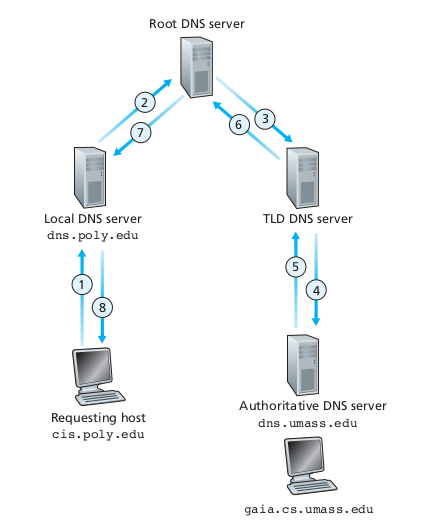
\includegraphics[scale=0.50]{recursiveDNSQueries}
  \caption{Recursive queries in DNS}
  \label{fig:recursive-dns-queries}
\end{figure}

\begin{figure}[tbp]
  \centering
  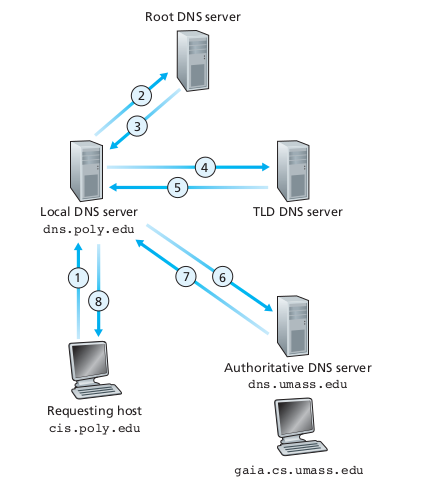
\includegraphics[scale=.50]{recurIteraDNSQueries}
  \caption{Iterative and recursive queries in DNS}
  \label{fig:itera-recur-quer-dns}
\end{figure}

\section{DNS Cache}
\label{sec:dns-cache}

Upon receving authorative results from upper level, a name server
chooses to \textbf{cache} the mapping results for a fixed period
(the 2nd column of \lstinline|dig| output), within which, new
matched queries are served immediately. DNS caching can manifestly
reduce DNS resolution time and improve user experience.

Although a domain name can be resolved by different domain name
servers with DNS cache, those servers must have an authorative
source (check SOA in section \ref{sec:zone-data-file}).

\section{Round Robin}
\label{sec:dns-round-robin}

Round Robin is a technique of load distribution/balancing,
provisioning multiple and redundant service hosts by managing DNS
responses to address queries.

Most network application have a list of backend hosts and IPs
thereof. The order of IPs returned are permuted in a round robin
way.

Generally, a client application just pick the very first IP from
the reply, so that different clients would receive service from
different backends, thus distributing the overall load among
servers.

\section{Anycast}
\label{sec:dns-anycast}

Apart from Round Robin, the system also adopts
\href{https://en.wikipedia.org/wiki/Anycast}{Anycast} to eliminate
the bottleneck of 13 root name servers. Name server IP has a bunch
of backend hosts.

With the help of BGP routing and Automation System (AS), DNS
queries are distrubted to a geographically nearby host.

\section{Zone Data File}
\label{sec:zone-data-file}

RRs are actually defined in \textit{zone data file}s of name
servers. As mentioned, a domain name server cannot have all the
records of the whole database. A zone data file contains only part
of the complete database. The term zone is analogous to domain,
but not identical. For example, a zone data file may contain only
part of RRs for a domain.

Basically, there are two types of zone data file. One is in the
form of \uline{db.DOMAIN} that maps domain names to IPs, which is
called \textit{forward mapping}. Take domain name
\textit{bing.com} for example, forward mapping records are stored
in file \textit{db.bing.com}.

The other type is for \uline{reverse mapping} that maps IPs to
domain names in the form of \uline{db.ADDR}, where \uline{ADDR} is
the network address without trailing zeros. Take block
\textit{192.249.249.0/24} for example, its zone data file is
\textit{db.192.249.249}. Records in this type are called
\href{https://en.wikipedia.org/wiki/Reverse_DNS_lookup}{PTR}.

Zone data files are also called \textit{db} files. Any DNS
implementation (i.e. BIND and Dnsmasq) must have these zone data
files to support lookups. Also, they must comply with the same
data format - \uline{master file format}
\ref{sec:master-file-format}.

How these files are organized and located depends on
\uline{connfiguration file}. For BIND 8 or 9, the configuration
file is \textit{/etc/named.conf}. The format of configuration file
is flexible and depends on implementations.

\section{Master File Format}
\label{sec:master-file-format}

Text after semicolon to the end of a line is treated as
comments. Code \verb|$TTL| set the cache time of a record.

Start of Authority (SOA) record is a must for every domain name
server, indicating this server is the \textit{best} source of
information for the data within this zone. There can be one and
only one SOA record in each a data zone file.

Here is an excerpt of a SOA query for
\textit{www.bing.com.}. Obviously, db files on servers
\textit{ns1.cn-msedge.net.} and \textit{msnhst.microsoft.com.}
should contain such SOA record.

\begin{lstlisting}
; dig www.bing.com soa
cn-msedge.net.		59	IN	SOA	ns1.cn-msedge.net. msnhst.microsoft.com. 2017032701 1800 900 2419200 240
\end{lstlisting}

SOA record is also used to do zone data file
\href{https://en.wikipedia.org/wiki/DNS_zone_transfer}{synchronization}
periodically among distributed domain name servers in the
system. Ideally, each server should cache as many RRs as
possible. However, it is infeasible as the size is too much to
hold and the increased synchronization traffic is beyond
negligibleness.

Pointer (PTR) record accomplishes reverse mapping. The firstly
field is a concatanation of a reverse network address and suffix
domain \textit{in-addr.arpa}. PTR records must point to
\textit{canonical} domain names instead of aliases:

\begin{lstlisting}
; dig -x 204.79.197.200
200.197.79.204.in-addr.arpa. 2806 IN	PTR	a-0001.a-msedge.net.
\end{lstlisting}

In a \uline{db.domain} file, symbol \verb|@| can be used to
replace current ORIGIN. For example, a MX record \ref{lst:mx-rr}
usually starts with \verb|@|:

\begin{minipage}{1.0\linewidth}
\begin{lstlisting}[caption={MX RR},label={lst:mx-rr}]
# db.movie.edu
@ IN SOA terminator.movie.edu. al.robocop.movie.edu. (
                          1h   ; serial number
                          3h   ; refresh after 3 hours
                          1h   ; retry after 1 hour
                          1w   ; expire after 1 week
                          1h ) ; negative expiration
\end{lstlisting}
\end{minipage}

\section{Resolver}
\label{sec:dns-resolver}

Once DNS is implemented, how to make use of it? We need
\textit{resolver}. Resolvers are the clients that access name
servers when any programs running need name resolution.

Resolvers require configuration (\verb|/etc/resolv.conf|)
beforehand and allow customization of the following items:

\begin{itemize}
\item default \textit{domain} directive;
\item \textit{search} list directive;
\item \textit{nameserver}s directive;
\item \textit{sortlist} directive;
\item \textit{optoin}s directive.
\end{itemize}

The \textit{domain} and \textit{search} directives are mainly used
to make users' lives easier by saving them some typing. Both
directives generate a list of relative domain names. When domain
names sent to the resolver are relative (not FQDN), it would
prepend the input to the each relative domain name in the
list. The resulted domain names sent to namer servers is still
relative, and will be appended by current ORIGIN.

%%% Local Variables:
%%% mode: latex
%%% TeX-master: "main"
%%% End:

\chapter{HTTP}
\label{cha:http}

\href{https://tools.ietf.org/html/rfc2616}{Request for Comments -
  RFC2616} is now replaced by the \uline{723x} series, of which
\href{https://tools.ietf.org/html/rfc7230}{RFC7230} is the
starting point, defining HTTP message and message routing.

\section{Glossary}
\label{sec:http-glossary}

HTTP was created for the World Wide Web (WWW) architecutre, and
much of the architecture is reflected in the terminology and
syntax defined in RFC723x series.

HTTP is a \textit{stateless} protocol that operates by exchanging
messages over \uline{transport-layer} or \uline{session-layer}
connection in a \textit{client-server} mode.

\textit{client} and \textit{server} refer to only the
\textit{role} that HTTP \textit{program}s perform for a
\textit{particular} connection. The same program might act as a
client on some connections or a server on others. A client
\textit{establish}es a connection for the purpose of sending one
or more \textit{request}s, a server instead \textit{accept}s
connections in order to serve requests by sending
\textit{response}s.

\textit{connection} means a transport-layer connection of TCP/IP
protocol stack between two endpoints. \textit{endpoint} is either
the client or server side of the connection. \textit{peer} is a
\textit{remote} endpoint. \textit{request} from client and
\textit{response} from server emphasize data transmission.

\textit{user agent} refers to any of the various \textit{client
  program}s on behalf of end users, including but not limited to
browsers (i.e. Firefox), spiders (web-based robots like
Googlebot), command-line tools (i.e. Curl), custom applications,
and mobile apps.

The term \textit{origin server} refers to the \textit{server
  program} that can \textit{originate} authorative responses for a
target resource.

An \textit{entity} is comprised of \textit{entity header}s and
\textit{entity body}. \textit{entity body} and \textit{payload}
both refer to the body part of a HTTP message like equation
\eqref{eq:message-body}. But entity emphasizes the data
representation of target resource while payload emphasizes syntax
of HTTP message.

\begin{equation}
  \label{eq:message-body}
  \begin{aligned}[t]
    \text{message-body} &= \text{Transfer-Encoding(entity-body)} \\
                        &= \text{Transfer-Encoding(Content-Encoding(Content-Type(target-resource)))}
  \end{aligned}
\end{equation}

\textit{target resource}, on the contrary, means the contents
stored on origin server. For each content, the server might have
multiple \textit{representation}s reflecting different versions of
the content, like modification date, compression etc. In other
words, a content may have multiple target resources that in turn
may have multiple entities.

HTTP supports the use of \textit{intermediaries} to satisfy
requests through \textit{a chain of connections}. There are three
common intermediaries: \textit{proxy}, \textit{gateway}, and
\textit{tunnel}. In some cases, a single intermediary might change
its type among proxy, gateway and tunnel based on the nature of
each request.

Terms \textit{upstream} and \textit{downstream} are used to
describe directional requirements in relation to \textit{message
  flow} regardless of requests or reponses: all messages flow from
upsteam to downstream. \textit{inbound} and \textit{outbound} are
used to describe directional requirements in relation to the
reponse: inbound means downstream response from the origin server
and outbound means downstream response to the user agent.

Proxy refers to \textit{forwarding proxy} and Gateway refers to
\textit{reverse proxy}. A proxy is a messsge-forwarding agent
selected by clients. A gateway acts as an origin server for
outbound connections but translates received requests to another
server, which is transparent to clients. Gateways are often used
to do CDN for performance improvement, load balancing across
multiple machines. Check the 502 (Bad Gateway) status code in
section \ref{sec:server-error-5xx}.

A proxy or gateway is defined in the context of HTTP
communication. There are also proxies that can act on
\textit{lower} layers of the network protocol stack, filtering or
redirecting HTTP traffic without the knowledge or permssion of
HTTP participants. For example, \textit{interception proxy} (also
commonly known as \textit{transparent proxy}) is selected by
neither client nor server sides.

A tunnel is just a \textit{blind relay} between two connections
without changing the messages. Once active, a tunnel is not
considered a party to the HTTP communication. The tunnel is not
aware of any HTTP syntax or semantics.

Before ending this section, let's recall the term stateless. This
term means each request can be understood or parsed standalone,
withou any prior knowledge. A server MUST NOT assume that two
requests on the same connection are from the same user
agent. Specially, the ``stateless'' feature enables reuse of
\textit{cache}, and load balancing across multiple servers.

\section{Cache}
\label{sec:http-cache}

A cache is a local store of previous response messages and
a relevant subsystem that controls its storage, retrieval, and
deletion.

The purpose of a cache is to store \textit{cacheable} responses in
order to reduce the \textit{response time} and network
\textit{bandwidth consumption} on future, equivalent
requests. Please pay attention, not all reponses are cacheable
such as that of POST and PUT (read more in section
\ref{sec:put-post}.

The effect of a cache is that the request/response chain is
shortened if one of the intermediaries along the chain has a
cached response applicable to that request like figure
\ref{fig:shortened-http-chain}.

\begin{figure}[bp]
  \centering
  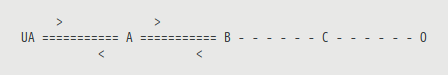
\includegraphics[scale=0.5]{shortened-http-chain}
  \caption{Shortened HTTP Chain}
  \label{fig:shortened-http-chain}
\end{figure}

\subsection{URL URI}
\label{sec:url-uri}

URI is the superset of URL in general. However, within an URL, the
part after the domain name (including the leading forwardslash) is
also a type of URI which, in RFC, is called \textit{resource
  identifier}.

\href{https://stackoverflow.com/q/28592077}{Regarding Nginx},
vairable \verb|request_uri| is the equivalent of URI while
variable \verb|uri| is the normalized \verb|request_uri| without
query string.

\section{HTTP Method}
\label{sec:http-method}

\subsection{PUT POST}
\label{sec:put-post}

\href{https://stackoverflow.com/a/630475}{POST and PUT} both can
be used for \textit{creating} and \textit{updating} resources on
servers.

PUT sends an entity with a specified URI location to the
server. If there already exists an entity on that URI, it will be
updated (replaced by the new one). Otherwise, the new entity is
created (put) on the server. So we know that the PUT method
requires an given URI identifier in the request.

PUT is \textit{idempotent} (幂等) similar to variable assignment
like \verb|x = 5|. If an entity are put multiple times, it makes
no difference and the result is guaranteed.

POST is almost the same as PUT but cannot be used to to create a
new entity on a given URI. That is to say, the identifier part of
an URI when creating is determined by the server side
semantics. For example, this request would probably receive a 4xx
status code (probably 404) when creating a new question to
\textit{stackoverflow.com}:

\begin{lstlisting}
POST /questions/http-put-vs-post HTTP/1.1
Host: stackoverflow.com
\end{lstlisting}

Instead, please remove the resource identifier:

\begin{lstlisting}
POST /questions/ HTTP/1.1
Host: stackoverflow.com
\end{lstlisting}

The server will create the resource identifier on
demand. Therefore, POST creates a \textit{subsidiary}
resource. Here is an excerpt from the Internet:

\begin{quotation}
  From the other side of the fence: PUT if the client determines
  the resulting resource's address, POST if the server does it.
\end{quotation}

Apparently, POST is \textit{not idempotent} when \textit{creating}
the same entity multiple times as the identity part is not
controlled by the client side, resulting in duplicate entities
located under different URIs.

As both PUT and POST create or update entities, reponses are
\textit{not} cacheable as those operations are expected to execute
\textit{only once} by nature. If a PUT or POST request was cached,
then cache servers (including user agents) would repeat the
request unintentionally and the relevant entity would be created
or updated repeatedly too. To the contrary, a GET method only
reads entity from servers and can be cached.

\subsection{GET POST}
\label{sec:get-post}

The advantage of GET over POST is that everything about a GET
request is stored in the URI. So it is quite easy to be
manipulated on the fly; recorded by search engine; bookmarked by
browser; cached by proxy etc.

In terms of method security, POST is advantageous over GET. When
GET something from the server, the request URI can be tracked
through browser history, server log and search engine
(i.e. Google) . On the other hand, desired action of POST method
is embedded in the message body and cannot be cached. However,
both methods use plain text transfer and can sniffed easily unless
HTTPS is adopted.

\section{HTTP Response Status Code}
\label{sec:http-response-status-code}

In this section, \textit{response code}, \textit{status code}, and
\textit{response status code} are referred to interchangeably, and
mean almost the same thing: an three-digit integer from web server
indicating the request and reponse status. The name
\textit{response} represents the HTTP reply message.

\begin{figure}[tbp]
  \centering
  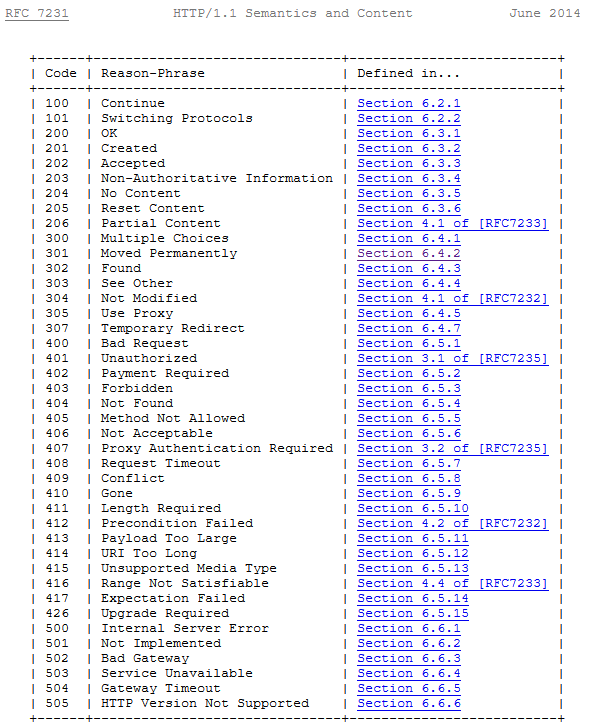
\includegraphics[width=.60\textwidth]{http-status-code}
  \caption{HTTP Status Code}
  \label{fig:http-status-code}
\end{figure}

For authorative reference, check
\href{https://tools.ietf.org/html/rfc7231/rfc7231}{RFC7231}. Figure
\ref{fig:http-status-code} defines the list of available official
codes. They are grouped into five categories, with the first digit
defining the code class:

\begin{itemize}
\item 1xx \textit{informational response}: the request was
  received, continuing process.
\item 2xx \textit{successful response}: the request was
  successfully received, understood, and accepted.
\item 3xx \textit{redirect}: futher action needs to be taken in
  order to complete the request.
\item 4xx \textit{client error}: the request contains bad syntax
  or cannot be fulfilled.
\item 5xx \textit{server error}: the server failed to fulfill an
  apparently valid request.
\end{itemize}

HTTP clients are not required to understand all registered status
codes, though such understanding is obviously desirable. However,
a client MUST understand the class (namely, the first digit) of
any received code, and treat an unrecognized status code as being
equivalent to the x00 status code of the x class where x belongs
to ${1,2,3,4,5}$, with the exception that a \textit{recipient}
(i.e. proxy server) MUST NOT cache a response with an unrecognized
status code.

Responses with status codes (by default, 200, 203, 204, 206, 300,
301, 400, 404, 410, 414, and 501) can be cached for hueristic
expiration unless otherwise indicated the method definition or
explicit cache
controls. \href{https://tools.ietf.org/html/rfc7234}{RFC7234}
defines HTTP caches and the associated header fields that control
cache behavior or indicate cacheable response messages.

\subsection{Informational 1xx}
\label{sec:informational-1xx}

The 1xx class of status code indicates an \textit{interim}
response for communicating connection status or request progress
\textit{prior} to completing the requested action and sending a
final response.

The 100 (Contine) status code indicates that the initial part of a
request has been received and has not yet been rejected by the
server. The server intends to send a final response after the
request has been fully reeived and acted upon.

The 101 (Switching Protocols) status code indicates that server is
willing to change application protocol like upgrading to a newer
HTTP version.

\subsection{Successful 2xx}
\label{sec:successful-2xx}

The 2xx class of status code is mostly desired, indicating the
request was successfully received, understood, and accepted.

Of the 2xx class, the 200 (OK) status code is what a client
expects largely and always (except the CONNECT method) has a
payload, though an origin server MAY generate a payload body of
zero length.

The 201 (Created) status code indicates that the request has been
fulfilled and one or more new resources have been created (PUT,
POST etc. methods).

The 202 (Accepted) status code indicates that the request has been
accpeted for processing, but the processing has not been
completed.

The 203 (Non-Authoritative Information) status code indicates that
the request was successful but the enclosed payload has been
modified by a transforming proxy. For example, image format is
changed in an intermediate web proxy.

The 204 (No Content) status code indicates that the server has
successfully fulfilled the request and that there is no additional
content to send in the response payload body (PUT, POST
etc. methods). Action is successfully applied to the server and
the user agent will inform its user the success (i.e. a dialog pop
up).

\href{https://tools.ietf.org/html/rfc7233}{The 206 (Partial
  Content)} code means the server is successfully fulfilling a
range request for the target resource by transferring one or more
parts of the selected representation that corresponds to the
satisfiable ranges found in the request's Range header field.

\subsection{Redirection 3xx}
\label{sec:redirection-3xx}

The 3xx (Redirection) class of status code indicates that further
action needs to be taken by the user agent in order to fulfill the
request. Most of the time, the user agent will send another
reqeust to the new URI specified in Location header field in the
response.

User agents diverge on the method applied to the second
request. In HTTP 1.0, 301 (Moved Permanently) and 302 (Found) are
defined to use the same method as the original reqeust, while 303
(See Other) rewrites method as GET regardless of the original
method. However, most user agent implementations always rewrite
the method as GET despite 301, 302 or 303.

Considering the implementation prevalence, HTTP/1.1 \textit{has
  to} acknowledge the de facto practice, and added 307 (Temporary
Redirect) and 308 (Permanent Redirect) to \textit{explicitly}
disallow method rewrite. In other words, original POST method
cannot be rewritten to GET. Table
\ref{tab:redirect-and-method-rewrite} is a summary of method
rewrite from \href{https://tools.ietf.org/html/rfc7231}{RFC7231}
and \href{https://tools.ietf.org/html/rfc7238}{RFC7238}.

\begin{table}[tbp]
  \centering
  \begin{tabular}[tbp]{c|c|c}
    \toprule{}
    Method & Permanent & Temporary \\
    \midrule{}
    POST to GET & 301 & 302 \\
    POST & 308 & 307 \\
    GET & & 303 \\
    \bottomrule
  \end{tabular}
  \caption{Redirect and Method Rewrite}
  \label{tab:redirect-and-method-rewrite}
\end{table}

Permanent redirect means future requests of the target resource
should be sent to the new URI while temporary redirect sticks to
the old URI. When upgrading HTTP to HTTPS or switching
\textit{php} to \textit{html}, 301 permanent redirect can be
adopted. The 302 status code can be classified into
\textit{on-domain} redirect (same domain name) and
\textit{off-domain} redirect (different domain name). For example,
users are usually redirected to a login URI temporary. Regardless
of 301 or 302, domain name redirect is discouraged, which requires
proper design at the very beginning of service deployment.

The 303 (See other) redirect explicitly rewrites request method as
GET/HEAD to \textit{retrieve} the target resource, and does not
imply permanent or temporary redirect. Name ``retrieve'' is chosen
as the new URI in the response is intended to provide only
\textit{descriptive} information on the final
target. Consequently, 302 redirect is also called \textit{indirect
  redirection} as further redirections may be required.

The redirect difference between 301 and 302 make a difference when
Search Engine Optimization (SEO) is concerned. If domain name
change is done with 301 redirect, then the Page Ranking (PR) of
the old domain name is probably lost. When a 302 redirect is
encountered, search engine by default attributes the page ranking
to the original URI. Search engines may downgrade the PR as a
target resource is preferred to be located by an unique URI.

Specially, 302 redirect is utilized to do
\href{https://en.ryte.com/wiki/URL_Hijacking}{URL Hijacking},
basically, stealing PR of another domain for the favor of
hijackers' page contents. At the very beginning, a hijacker should
find a way to achieve 302 redirect. For example, hack the target
web server and embed a 302 directive directly in the HTML file or
through Nginx \textit{rewrite} directive. Other methods are like
\href{https://blog.csdn.net/mgxcool/article/details/47206835}{DNS
  Hijacking},
\href{http://xsk.tehon.org/den/index.php/category/tech/tcp-bypass-hijacking-feature-and-recognization.html}{Bypass
  Interception} etc. When a user searches keywords covered in the
hijacker's page, search engine would probably return the original
URL that would be then redirected to the hijacker's URL. Once
succeeded, the PR of the original page is contributed to the
hijacker's page.

Another interesting code is 304 (Not Modified). This code is
returned when a conditional GET or HEAD request is received but
the condition is evaluated to false. In other words, the target is
not modified and the user agent has a up-to-date representation of
the target resource. There is no need to transfer another
representation of the target resource. Therefore, the 304 response
\textit{must not} contain a message-body.

More details,
please check section \ref{sec:last-modified}.

\subsection{Client Error 4xx}
\label{sec:client-error-4xx}

The 4xx class indicates the client seems to have erred. The 400
(Bad Reqeust) status code means the server cannot fulfill the request due to
malformed request syntax, invalid URI, deceptive request routing
etc.

401 (Unauthorized) indicates that the request has not been applied
because it lacks valid authentication credentials for the target
resource. 403 (Forbidden) indicates that the server understands
the request but refuses to authorize it like invalid credentials.

404 (Not Found) indicates the server cannot find a
current representation for the target resource or is not willing
to disclose existence.

410 (Gone) indicates access to the target resource is no longer
available (i.e. removed) at the origin server. It is common for
limited-time, promotional services and for resources belonging to
individuals no longer associated with the origin server's site.

405 (Method Not Allowed) indicates that the method recevied in the
request-line is known by the origin server but not supported by
the target resource.

416 (Range Not Satisfiable) indicates none of the ranges in the
request's Range header field \textit{overlap} the current extent
of the selected resource.

\subsection{Server Error 5xx}
\label{sec:server-error-5xx}

The 5xx (Server Error) class indicates that the server is aware
that it has erred or is incapable of performing the requested
method. The 500 (Internal Server Error) code indicates the server
encountered an unexpected condition that prevented it from
fulfilling the request. The 501 (Not Implemented) code means the
server does not support the functionality required to fulfill the
request.

The 502 (Bad Gateway) status code means the server, while acting
as a proxy or gateway, received an invalid response from an
inbound (upstream direction) server it accessed while attempting
to fulfill the request. The 504 (Gateway Timeout) code indicates
that the server, while acting as a gateway or proxy, did not
receive a timely response from an upstream server it needed to
access in order to complete the request.

The 503 (Server Unavailable) indicates the server is currently
unable to handle the request due to temporary overload or
scheduled maintenance. The situation might be allievated after
some delay.

\section{Headers}
\label{sec:http-headers}

\subsection{Last-Modified}
\label{sec:last-modified}

\uline{Last-Modified} is a reponse header field providing a
timestamp indicating the date and time at which the origin server
believes the selected representation was last modified.

\uline{If-Modified-Since} is a request header field, making the
entity transfer conditional on the modification date of remote
version being more recent than the field value.

When a cache party is involved, it will typically use the value of
the cached message's Last-Modified field to generate
If-Modified-Since. However, occasionally, other source data might
be used such as the \uline{Date} header field of the cached
message.

The combination of Last-Modified and If-Modified-Since limits the
scope of a web traversal to resources that have recently changed
and reduce bandwidth.

\subsection{ETag}
\label{sec:etag}

\uline{ETag} is another response header field providing the
current \textit{entity tag} for the selected representation, as
determined at the conclusion of handling the request. It is an
opaque string (i.e. a MD5 hash) differentiating between multiple
representations of the same entity.

Similar to the Last-Modified and If-Modified-Since pair, a client
can also use ETag values using If-Match or If-None-Match (analyzed
below) to do conditional requests and may save bandwidth and
response time. However, ETag is more reliable than date value when
it is inconvenient to store modification dates or when date values
is not accurate due to clock synchronization

The preferred behavior for an origin server is to send both a
strong entity-tag and a Last-Modified value in successful
responses to a retrieval request.

\subsection{If-None-Match}
\label{sec:if-none-match}

The \uline{If-None-Match} header field makes the request method
conditional on a recipient cache or origin server either not
having any current representation of the target resource when the
field value is '*', or having a selected representation with an
entity-tag that does not match any of those listed in the field
value.

Most of the time, the field value is set to be a list of cached
entity-tags. The server only responses a representation of which
the entity-tag does not appear in the list.

The special asterisk can prevent unsafe methods (i.e. PUT and
POST) from creating or updating a target representation multiple
times, resulting in ``lost update'' issue as any entity-tag on the
server will match the wildcard '*'.

On the other hand, there is the \uline{If-Match} header field in a
request. Upon receiving such requests, the server only performs
the method when the representation entity-tage match any of the
field value. If the value is wildcard '*', it requires at least
one representation exist.

Table \ref{tab:condi-hed-cache-vld} shows the combination of
conditional headers.

\begin{table}[tbp]
  \centering
  \begin{tabular}[tbp]{r|l}
    \toprule
    Request Header & Reponse Header \\
    \midrule         
    If-Match & Etag \\
    If-None-Match & Etag \\
    If-Modified-Since & Last-Modified \\
    \bottomrule
  \end{tabular}
  \caption{Conditional Header and Cache Valiador}
  \label{tab:condi-hed-cache-vld}
\end{table}

\subsection{Forwarded}
\label{sec:http-forwarded}

\uline{Forwarded} is an \textit{extended} and \textit{optional}
HTTP \textit{header field} that, when used, contains a list of
\uline{parameter:identifier} pairs that disclose information
\uline{for} the \textit{client}, about the \uline{host} header
field and/or the \uline{proto}, or \uline{by} \textit{proxies}
when one or more proxies are involved in the chain of
\textit{request} connections

This header field is only used for HTTP requests and is not to be
used in HTTP responses. Due to the sensitive nature of disclosed
information, this header field should be turned off by
default. Further, it applies to reverse proxies, as well as
forwarding proxies. The following are samples added by a proxy:

\begin{lstlisting}
Forwarded: for="_gazonk"
Forwarded: For="[2001:db8:cafe::17]:4711"
Forwarded: for=192.0.2.60;proto=http;by=203.0.113.43
\end{lstlisting}

The identifier is a
\href{https://tools.ietf.org/html/rfc7239#section-6.3}{Obfuscated
  Identifier} that keep the IP address secret, while still
allowing the ``Forwarded'' header field to be used for tracing and
debugging.

From
\href{https://tools.ietf.org/html/rfc7230#section-3.2}{RFC7230}, a
\textit{header field} consists of a \textit{case-insensitive}
field name followed by a colon (\uline{:}), optional leading
whitespace, the field value and optional trailing whitespace. The
field name ``Forwarded'' can be written as lower case
``forwarded''. Pay attention please, \textit{parameter}s in the
field value are also case-insensitive. So ``for'' and ``For'' are
equivalent.

Pairs should be semicolon-separated within the field value
part. Each parameter must not occur more than once per field
value. In other words, an individual proxy can add only one
instance of a particular parameter.

A subsequent proxy that wants to add a new field value can either
append it to the last field value after a \textit{comma
  separator}, or add another ``Forwarded'' header field. Here is
an example:

\begin{lstlisting}
Forwarded: for=192.0.2.43, for=198.51.100.17
\end{lstlisting}

The two \uline{for} pairs are separated by a comma, representing
two field values added different proxies in the request chain.

For the list of field values, the very first field value is added
by the very first proxy, and each subsequent field value is
appended by each subsequent proxy. The \uline{for} parameter for
the last proxy in the chain is not required, as the upstream
server get its IP from the TCP connection directly.

A proxy can add a set of \uline{parameter:identifier} pairs; it
can also remove existing pairs added by previous proxies. Because
this header field is optional, any proxy in the chain may choose
not to update this header field. Please read more details from
\href{https://tools.ietf.org/html/rfc7239}{RFC7239}.

However, in reality, the ``Forwarded'' header field name is
implemented as \textit{X-Forwarded-For}. Nginx has two relevant
built-in variables to record the field value, namely
\lstinline|$proxy_add_x_forwarded_for| and
\lstinline|$http_x_forwarded_for|. The syntax is a bit different
from what is specified in the RFC. Here is a common setting on a
reverse proxy:

\begin{lstlisting}
proxy_set_header            X-Forwarded-For $proxy_add_x_forwarded_for;
\end{lstlisting}

Both variables may or may not be related to another built-in
variable \lstinline|$remote_addr| which is the IP address of the
preceding origin in the chain, derived from the underlying TCP
connection. Basically,
\lstinline|$proxy_add_x_forwarded_for| will \textit{append}
\lstinline|$remote_addr| to
\lstinline|$http_x_forwarded_for| that is the received field value
of ``X-Forwarded-For'' from the preceding origin in the chain. If
the Nginx is the very first proxy, then
\lstinline|$http_x_forwarded_for| would be empty.

By the way, the field value of ``X-Forwarded-For'' can be forged
easily by manipulating the request header:

\begin{lstlisting}
curl http://www.example.com -H 'X-Forwarded-For: a.b.c.d' -H 'X-Real-IP: e.f.g.h'
\end{lstlisting}

Often, the ``X-Forwarded-For'' is accompanied by another optional
field \uline{X-Real-IP} that records the
\lstinline|$remote_addr| like:

\begin{lstlisting}
proxy_set_header            X-REAL-IP $remote_addr;
\end{lstlisting}

Unlike the \textit{add} or \textit{append} nature of
\lstinline|$proxy_add_x_forwarded_for|, \uline{X-REAL-IP} is
always overwriten by the current proxy. So it cannot be forged by
manipulating the request header.

\section{CORS}
\label{sec:cors}

The \textit{name} \uline{origin} refers to a \textit{tuple}
consisting of \textit{protocol}, \textit{domain} and
\textit{port}:

\begin{lstlisting}
(protocol, domain, port)
\end{lstlisting}

It is a property derived from web URL. Any variation of the three
values denotes a different origin. Two URLs have the \textit{same
  origin} if the protocol, domain, and port (if specified) are the
same for both. The two URLs below have different origin as the
ports are different.

\begin{lstlisting}
http://www.example.com/data/cat.jpg
https://www.example.com/data/cat.jpg
\end{lstlisting}

Script (i.e. JS) URLs in the form of \textit{about:blank} or
\textit{javascript:} do not define a origin as protocol, domain,
and port are \textit{all absent}. Such script \textit{inherit}s
the origin of the document containing the URL.

Before telling about what Cross-Origin Resource Sharing (CORS) is,
let's have a look at
\href{https://developer.mozilla.org/en-US/docs/Web/Security/Same-origin_policy}{same-origin
  policy}. It is a critical mechanism that restricts how a
document or script loaded from one origin can interact with a
resource from another origin.

We call interactions between different origins
\textit{cross-origin} access, such as when we use
\href{https://developer.mozilla.org/en-US/docs/Web/API/XMLHttpRequest}{XMLHttpRequest}. It
is a rule enforced by web browsers, not that of web servers. By
default, a web browser does not allow cross-origin HTTP requests,
where
\href{https://developer.mozilla.org/en-US/docs/Web/HTTP/CORS}{CORS}
comes into being. Figure \ref{fig:cors} gives a clear
illustration.

Loading the script file itself does \textbf{not} belong to
cross-origin access and is not restricted by the same-origin
policy. It is what the script executes after loading that do
cross-origin access.

\begin{figure}[!htb]
  \centering
  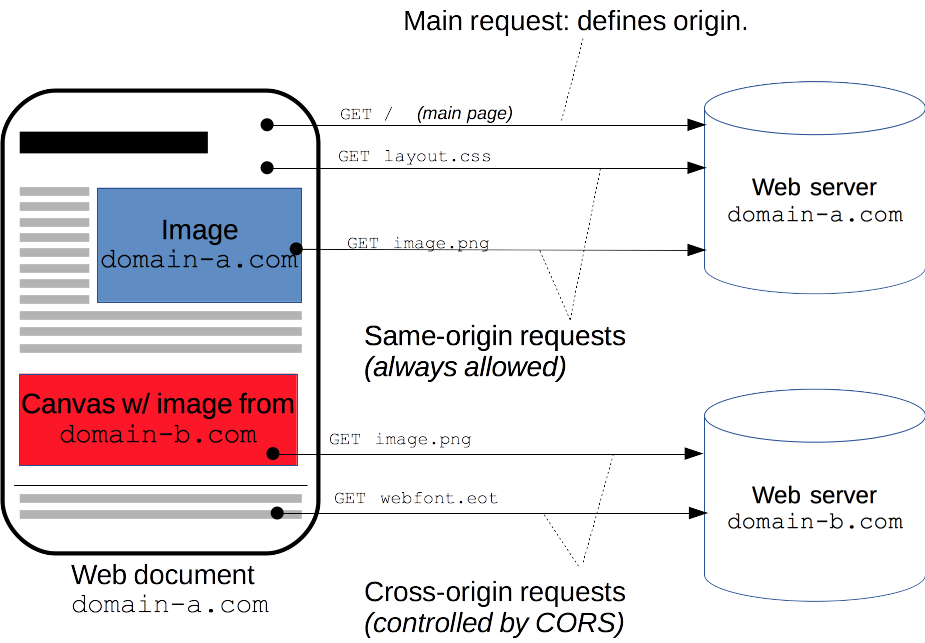
\includegraphics[width=.8\textwidth]{CORS_principle}
  \caption{Cross-Origin Resource Sharing}
  \label{fig:cors}
\end{figure}

CORS refers to Cross-Origin Resource Sharing, letting a web server
specify whether other web servers are permitted to load content
from it. It uses additional HTTP headers to tell a
\textit{browser} that a web application for one \textit{origin}
has permission to access selected resources from another web
application for a \textit{different origin}.

A web application should executes \uline{cross-origin HTTP
  request} when it requests a resource served by a different
origin than its own. Such requests cotain a HTTP header named as
\uline{Origin}. For example, the frontend Javascript code for a
web application served under the origin of
\uline{http://domain-a.com} uses XMLHttpRequest to make a request
for data \uline{http://api.domain-b.com/data.json}. The request
headers include \uline{Origin: http://domain-a.com} which
manifests how the term ``origin'' comes into being.

Whether the response is blocked or not by the broswer depends on
response header \uline{Access-Control-Allow-Origin}, indicating
whether the response can be shared with requesting code from the
given origin like:

\begin{lstlisting}
Access-Control-Allow-Origin: *
Access-Control-Allow-Origin: http://api.domain-b.com
Access-Control-Allow-Origin: null
\end{lstlisting}

The special wildcard \verb|*| means to allow CORS from any
origin. Apart from the simple XMLHttpRequest, CORS also supports
other methods like
\href{https://developer.mozilla.org/en-US/docs/Web/HTTP/CORS#Preflighted_requests}{Preflighted
  Request}. CORS is only one of the mechanisms to achieve
cross-origin access. There exists
\href{https://stackoverflow.com/q/2067472}{JSONP} to execute the
same will. However JSONP is almost outdated and you only require
it for older browsers.

简单用中文说:

\begin{itemize}
\item The Same-Origin Policy 叫同源策略。在没有同源策略之前,浏览器
  里不同源的代码和内容可以随意交互,不受限制。这会带来安全隐患,
  如 Origin A 的恶意代码可以访问 Origin B 上的安全信息。
\item 完全遵守同源测策也使 HTTP 应用灵活性降低。如同一 Origin 里的
  域名可以有很多别名 CNAME, 因此诞生了跨域(跨源)访问机制。其中一
  种就是本文讲的 CORS. 简单来讲,就是服务器端告诉浏览器,哪
  些Origin 可以对本 Origin 进行跨域访问。
\item Origin A 服务器上的 js 脚本以 CORS 方式抓取 origin B 服务器上
  的内容,浏览器会检查 B 的响应
  头 \text{Access-Control-Allow-Origin}, 如果响应头中包含 origin A
  则显示返回的内容,否则禁止。
\item Origin A 从 Origin C 加载 JS 脚本这个行为本身不属于跨域范筹,
  不受同源测策略限制。脚本在加载完毕后,对 Origin B 执行的请求才是
  跨域访问。
\item 跨域只存在于浏览器端,不存在
  于 android/ios/Node.js/python/java 等其它环境。跨域请求能发出去,
  服务端能收到请求并正常返回数据,只是结果可能被浏览器拦截了。如果
  需要禁止对服务器的访问,则需要上“防盗链”或“鉴权”。
\end{itemize}

\section{Websocket}
\label{sec:websocket}

The \href{https://tools.ietf.org/html/rfc6455}{websocket} protocol
is a different protocol from HTTP for its own purpose, though they
are related. Basically they are at the same layer over protocol
stack and both sit on top of TCP connection.

Websocket is created not to replace HTTP but to meet new web
requirements like \textit{high throughput} and \textit{low
  latency}. In order to be compatible with existing web
infrastructure, Websocket makes use of HTTP handshake by the
header fields \uline{Upgrade: websocket} and \uline{Connection:
  Upgrade} at port 80 or 443. Upon receving the HTTP handshake
request, the websocket server responds with status code 101
(Switching Protocols). From then on, the protocol is switched from
HTTP to websocket. All following transmission is carried over the
TCP connection just established. Like HTTP, it is a
\textit{message} protocol with each message 6 bytes
headers. However, 6 bytes is negligible compared to HTTP headers.

At the very beginning, Websocket is one of the features
(i.e. \uline{Local Storage} and \uline{Geolocation}) defined by
the \href{https://en.wikipedia.org/wiki/HTML5}{HTML5}
specification and is now moved to a standalone protocol to keep
the subjet focused. Hence, it is not unusual to call it
\uline{HTML5 Websocket}.

Next I will talk about the purpose of Websocket and why it is
invented alongside with HTTP. HTTP requires
\textit{synchronization} with strict \textit{request} and
\textit{response} pair order. only the \textit{client} side can
initiate the communication while the \textit{server} side
cannot. We call it a \uline{request/response protocol}.

A HTTP/1.0 TCP connection allows only one request sent out at any
given moment on a given TCP connection. After getting the
response, the TCP connection would be closed and the client can
send out a new request. However, a new TCP connection needs
created. Such a synchronized request and response method brings in
extra bandwidth and increases latency.

That is changed in HTTP/1.1 where the
\href{https://tools.ietf.org/html/rfc6223}{keep-alive} feature
keeps the underlying TCP connection open for further request and
response pairs. Therefore, it is also called
\href{https://en.wikipedia.org/wiki/HTTP_persistent_connection}{HTTP
  Persistent Connection}. Another feature of HTTP/1.1 is
\uline{HTTP pipeline}. Based on persistent connection, The client
do not have to wait for responses before sending out new
requests. So requests can sent out in line in series. However, the
responses must arrive in
\href{https://stackoverflow.com/a/34479053}{the exact order} as
requests. Therefore, it is not a true multiplexing method. Most
existing infrastructure (including Chrome/Firefox) disables HTTP
pipeline by default.

HTTP/1.1 introduces
\href{https://tools.ietf.org/html/rfc7230#section-3.3.1}{Transfer-Encoding}
mechanism, an interface towards the TCP socket. It us not unusual
we call it \uline{HTTP Streaming} as Transfer Encoding allows
sending of a resource representation in a set of \uline{chunk}s
sequentially. Chunks are sent and recived from the persistent TCP
socket. It is HTTP application's role to reassemble the
chunks. Upon receving all the chunks, the client reassembles them
as a whole - the response! Transfer-Encoding fits dynamically
generated content.

However, the \uline{request/response model} still cannot satisfy
modern real-time transmission requirements. The request and
response headers are still present but most of them are almost
identical - \textit{redundant} data. Also, the pipeline by nature
demands strict order! That is to say, the synchronization feature
is still present, which suffers from
\href{https://stackoverflow.com/q/45583861}{Head-of-Line (HOL}
blocking. If the very first request of the pipeline is somehow not
delivered as fast as expected, the requests behind are all
blocked!  Accordingly, clients (also applies to HTTP/1.0) need to
make many requests use multiple connections to a server in order
to achieve concurrency and thereby reduce latency.

On the other hand, Websocket is a \textit{asynchronous
  full-duplex} protocol designated for \textit{high throughput}
and \textit{low latency}. Firstly, it is a full-duplex
protocol. Once the TCP connection is established, it is ready for
data transmission from and to either side, regardless of client or
server, namely \textit{server push}. HTTP may utilize
\href{https://stackoverflow.com/q/12555043}{polling or long
  polling} (somehow a stupid workaround) or \textit{plugin}s like
\uline{Java Applet}, \uline{Flash}, and
\uline{Silverlight}. However, a plugin may not be accepted by
intermediaries (CDN, proxies or firewalls), require cusotom ports,
and is subject to security vulnerabilities. Websocket reuses
well-known port 80 or 443 to be compatible with exsiting web
deployment. When a firewall or proxy intermediate party is
detected, Websocket automatically sets up a tunnel to pass through
by issuing a HTTP \uline{CONNECT} method.

As you see, data is sent out on demand, which is also called
\textit{server push}. Once data is ready, it is pushed to the
client immediately. The asynchronization nature increases
throughput greatly as the request/response synchronization hazard
is relieved. Both sides can send data simultaneously. Figure
\ref{fig:websocket-vs-http} illustrates the transmission schemes
between Websocket and HTTP.

\begin{figure}[!htb]
  \centering
  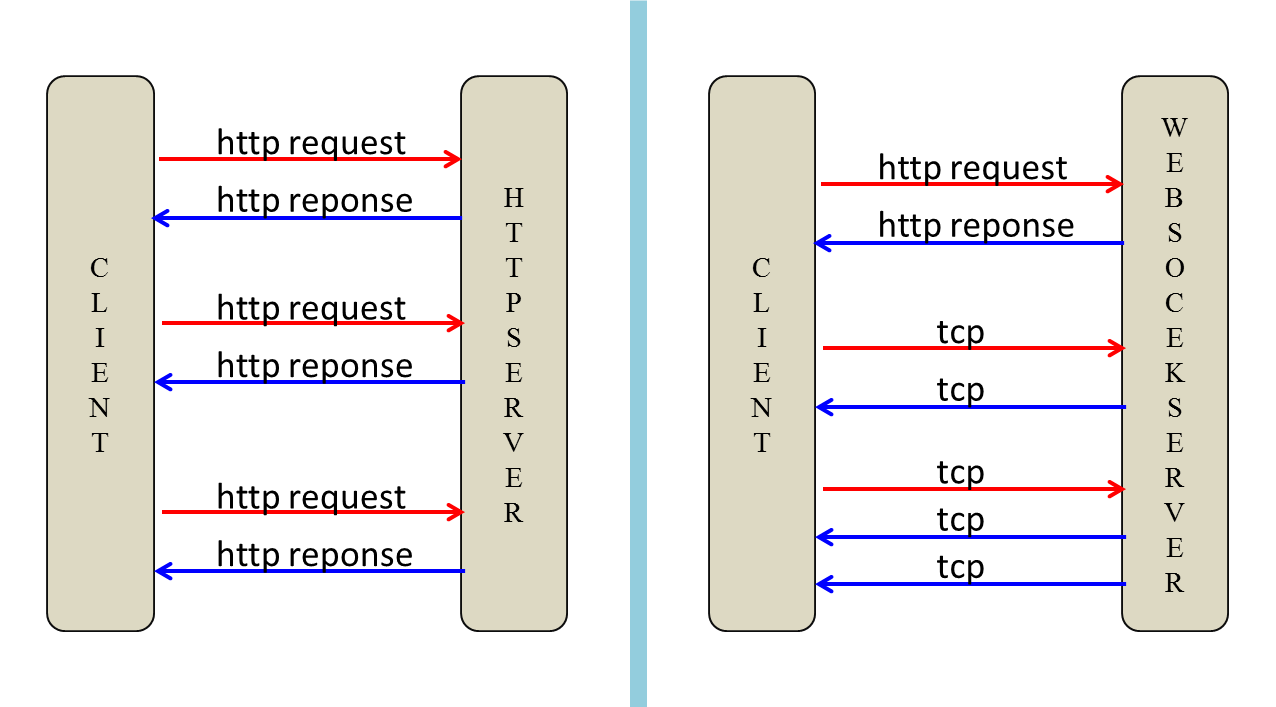
\includegraphics[scale=.5]{compareWebsocketHttp}
  \caption{Websocket vs HTTP}
  \label{fig:websocket-vs-http}
\end{figure}

With high throughput and low latency, Websocket fits application
like video games, stock trending, customer support, live streaming
etc. Whereas, HTTP has its own vantage points. It is much simpler
and has a well-supported ecosystem. Unless required, please resort
to HTTP first. Aslo, they can be combined together in live
streaming like \uline{HTTP+Websocket+FLV}. Figure
\ref{fig:live-streaming} shows the data flow of existing live
streaming applications.

\begin{figure}[!htb]
  \centering
  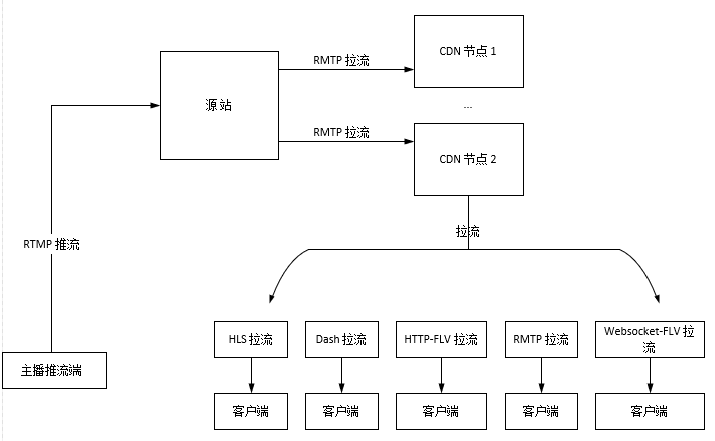
\includegraphics[scale=.5]{livestreaming}
  \caption{Live Streaming}
  \label{fig:live-streaming}
\end{figure}

To understand Websocket better, read
\href{http://www.importnew.com/28036.html}{再谈 Websocket 架构设计}
and \href{http://www.websocket.org/aboutwebsocket.html}{About
  Websocket}.

\section{HTTP/2}
\label{sec:http2}

In section \ref{sec:websocket}, we discussed the difference
between HTTP/1.0, HTTP/1.1 and Websocket. Websocket is an ideal
alternative to HTTP when serving applications of high throughput
and low latency like live streaming. However, it is \textit{less
  supported} by real world infrastructure compared with HTTP. That
is how HTTP/2 (not 2.0) comes into being. The name \uline{h2}
identifies the protocol where HTTP/2 over TLS while \uline{h2c}
identifies HTTP/2 over cleartext TCP.

HTTP/2 intends to be compatible with antecedent HTTP versions. So
all request/response semantics are preserved but the syntax of
conveying those semantics has
changed. \href{https://tools.ietf.org/html/rfc7540}{HTTP/2} is an
\textit{optimized} version of HTTP protocol. It improves
thourghput and reduces latency by introducing \uline{multiplexed
  request/response streams without HOL problems}, \uline{Header
  Compression, HPACK}, and \uline{unsolicited push of object
  representations from servers to clients}. All the benefits are
attributed to the \textit{binary frame} layer introduced between
HTTP and TCP. Different from the original text format, frame is
binary.

In the context of HTTP/2, a \uline{HTTP message} (either a request
or a response) is splitted to smaller parts as \textit{frame}s. A
frame refers to the \textit{smallest} unit of communication within
an HTTP/2 connection and consists of a header \footnote{the frame
  header, not the HTTP header} with 5 fields and a variable-length
(可变长) frame payload structured according to the \uline{frame
  type} field.

Frame type indicates the purpose of a frame. For instance, the
HEADERS frame and DATA frame form the basis of a HTTP message. The
HEADERS frame corresponds to \uline{HTTP header} while the DATA
frame corresponds to \uline{message payload}. Other frame types like
SETTINGS, WINDOW\_UPDATE, and PUSH\_PROMISE are used in support of
other HTTP/2 features. WINDOW\_UPDATE implements \textit{flow
  control}.

Header fields must be converted to lowercase within a HEADERS
frame before sending out. Due to the existence of DATA frames,
\textit{connection-specific} header fields like
\uline{transfer-encoding}, \uline{keep-alive},
\uline{Proxy-Connection}, \uline{Upgrade} etc. must \textbf{NOT}
be used in HTTP/2.

Another conecpt is \textit{stream} that is a
\textit{bidirectional} flow of frames within the HTTP/2
connection. Each stream consists of a set of frames, to realize a
request/response pair. A single HTTP/2 connection can contain
multiple concurrent streams, with either endpoint interleaving
frames along the connection. In other words, in the frame layer, a
stream represents a request/response exchange.

With so many frames over a HTTP/2 connection mangled, how to
identify the affiliations between frames and streams?
\uline{Streaming Identifier}! Frames of a particular stream is
identified by an integer assigned to by the endpoint initiating
the stream. The independency of streams solves the HOL blocking
issue. Frames of a stream can arrive in an intermingled way.

HTTP/2 \textit{interleaves} requests and responses over a single
persistent TCP connection with the requirement of
\href{https://stackoverflow.com/q/34478967}{pipeline order
  dismissed}. Exchange of request/response pairs is
\textit{independent} of one another and organized into
\uline{stream}s (discussed below). That is to say the exchange of
an individual request/response pair creates a new stream and close
it (a frame with the END\_STREAM flag set) once done. So the
blocking of a request/response pair of one stream does not prevent
the progress of pairs of other streams.

HTTP/1.1 only support compression of message body, but HTTP/2
extends this feature to header fields as well. Header compression
comprises of \uline{two index tables} and the \uline{static Static
  Huffman Encoding}, resulting a compression rate ranging from 0.5
to 0.95. The first index table is \uline{static table}, storing 61
predefined common headers like \verb|2 :method GET|,
\verb|3 :method POST| etc. The second is \uline{dynamic table},
storing variable or customized headers for host, uri etc. starting
from the index of 62. Huffman Encoding is a general
variable-length coding scheme that the higher the probability of a
event, the shorter its code is. From
\href{https://tools.ietf.org/html/rfc7541#appendix-B}{Static
  Huffman Encoding},
\begin{quotation}
  This Huffman code was generated from statistics obtained on a
  large sample of HTTP headers.
\end{quotation}

So the code for each character of headers is fixed, namely static,
in accord with historical data.

Like Websocket \ref{sec:websocket}, HTTP/2 supports \textit{server
  push} allowing a server speculatively sending data to a client
when the server anticipates that data is needed, namely response
\uline{before} request. This mechanism is a trade-off between
bandwidth and latency. If the unsolicted response is unwanted, the
bandwidth would be wasted. On the contratry, server push reduces
latency significantly.

HTTP/1.x uses the concept of \textit{start line}, namely the
\uline{request line} and \uline{response line}. However, HTTP/2
requires that all header fields a key-value pair. To be
compatible, HTTP/2 introduces \textit{pseudo-header fields}
beginning with colon \uline{:} giving each start line value a
name. Possible request pseudo-header names are \uline{:method},
\uline{:scheme}, \uline{:authority} (namely the \uline{host}),
\uline{path}, etc. URIs that do not contain a path component MUST
include a value of `/`. Remember that pseudo-header fields are not
standard HTTP header fields. \uline{:method}, \uline{:scheme} and
\uline{:path} are a must for HTTP/2 request. Every response must
have the \uline{:status} pseudo-header field.

\section{HTTP References}
\label{sec:http-references}

\href{http://www.ruanyifeng.com/blog/2016/08/http.html}{ruanyifeng http}

%%% Local Variables:
%%% mode: latex
%%% TeX-master: "main"
%%% End:
\chapter{ICT Operation}
\label{cha:ict-operation}

\lstset{language=bash}

\section{Cheat Sheet}
\label{sec:linux-cheatsheet}

Table \ref{tab:verify-linux-release} for release information;
\ref{tab:linux-account-management} for account information; table
\ref{tab:cmd-rock-tips} for handy tips.

\begin{table}[!htb]
  \centering
  \begin{tabular}[!htb]{l|l}
    \toprule
    Command & Usage \\
    \midrule
    \lstinline|fgrep -qa docker /proc/1/cgroup; echo $?| & Docker container \\
    \lstinline|cat /etc/{os,redhat}-release; rpm -q centos-release| & Distribution name \\
    \bottomrule
  \end{tabular}
  \caption{Verify Linux Release}
  \label{tab:verify-linux-release}
\end{table}

\begin{table}[!htb]
  \small
  \centering
  \begin{tabular}[!htb]{l|l}
    \toprule
    Command & Usage \\
    \midrule
    \lstinline|groupadd -g 2000 name| & Creata a group \\
    \lstinline|useradd -ms /bin/bash -u 1000 -g name name| & Create an account and specify the login group \\
    \lstinline|groupmod -g 1000 -n newname name| & Change group ID and name \\
    \lstinline|usermod -u 1000 -g newname -aG wheel name| & Change account ID, login group ID, and append to the 'wheel' group \\
    \lstinline/gpasswd [-a | -d] name name/ & Add or delete account 'name' to group 'name' \\
    \lstinline/getent [ passwd | group | hosts ]/ & Administrative database \\
    \lstinline|groups username| & Groups username joins \\
    \lstinline|users| & Users logged in to the system \\
    \lstinline|id| & Print uid, gid and groups \\
    \bottomrule
  \end{tabular}
  \caption{Linux Account Management}
  \label{tab:linux-account-management}
\end{table}

\begin{table}[!htb]
  \small
  \centering
  \begin{tabular}[!htb]{l|l}
    \toprule
    Command & Usage \\
    \midrule
    \lstinline|cat >> file.md << EOF| & Append contents to a file from STDIN with a \textit{here document} \\
    \bottomrule
  \end{tabular}
  \caption{Rock Tips}
  \label{tab:cmd-rock-tips}
\end{table}

\section{Linux Tools}
\label{sec:linux-tools}

\subsection{free}
\label{sec:linux-free}

\lstinline|free -hwt| commands display the amount of memory
allocations, by analyzing the contents of file
\lstinline|/proc/meminfo|:

\begin{lstlisting}[caption={Free Memory},label={lst:free-mem},basicstyle=\tiny\ttfamily]
              total        used        free      shared     buffers       cache   available
Mem:           3.7G        781M        1.5G        160M        558M        985M        2.8G
Swap:          1.0G          0B        1.0G
Total:         4.7G        781M        2.5
\end{lstlisting}

Always keep euqation:

$$\text{total} = \text{used} + \text{free} + \text{buffers} + \text{cache}$$

in mind.

\begin{itemize}
\item \textit{used} memory is allocated to user space processes.
\item \textit{free} memory is not allocated or freed up.
\item textit{shared} memory (mostly by \textit{tmpfs} is part of
  \textit{used}, shared among processes.
\item Kernel \textit{buffers} and \textit{cache} is allocated to
  kernel itself. \textit{cache} refers to memory used by the
  \textit{page cache} and \textit{reclaimable slab}s. For details
  about \textit{cache} and \textit{slab}, please read
  \ref{sec:os-memory}.
\item \textit{available} is the estimated amount of memory for
  starting new applications, \textit{without} swapping.
\end{itemize}

Ideally, \textit{available} should be the sum of \textit{free},
\textit{buffers} and \textit{cache}. However, \textbf{not all}
\textit{reclaimable slabs} can be freed in time as some may be in
use. So the actual \textit{available} size is slightly smaller.

%%% Local Variables:
%%% mode: latex
%%% TeX-master: "main"
%%% End:


\part{Algorithm}
\chapter{Tree}
\label{cha:tree}

\section{前序中序求后序}

给出一个二叉树的前序遍历 GDAFEMHZ 和中序遍历 ADEFGHMZ, 求后序遍历。
首先,二叉树的前序遍历,中序遍历,后序遍历的区别是根节点是先、中、
后访问。问题的关键是:

\begin{enumerate}
\item 前序遍历的第一个节点是根节点;
\item 在中序遍历里找到根结点,其左边是左子树节点,右边是右子树节点;
\item 对左子树重复上面两步;
\item 对右子树重复上面两步。
\item 二叉树被求出,从而得到对应的后序遍历。
\end{enumerate}

上面的例子里,从前序遍历知 G 是根节点,从后序遍历知,左子树是ADEF,
右子树是 HMZ, 此顺序就是左子树的中序遍历顺序。

\begin{figure}[h]
  \centering
  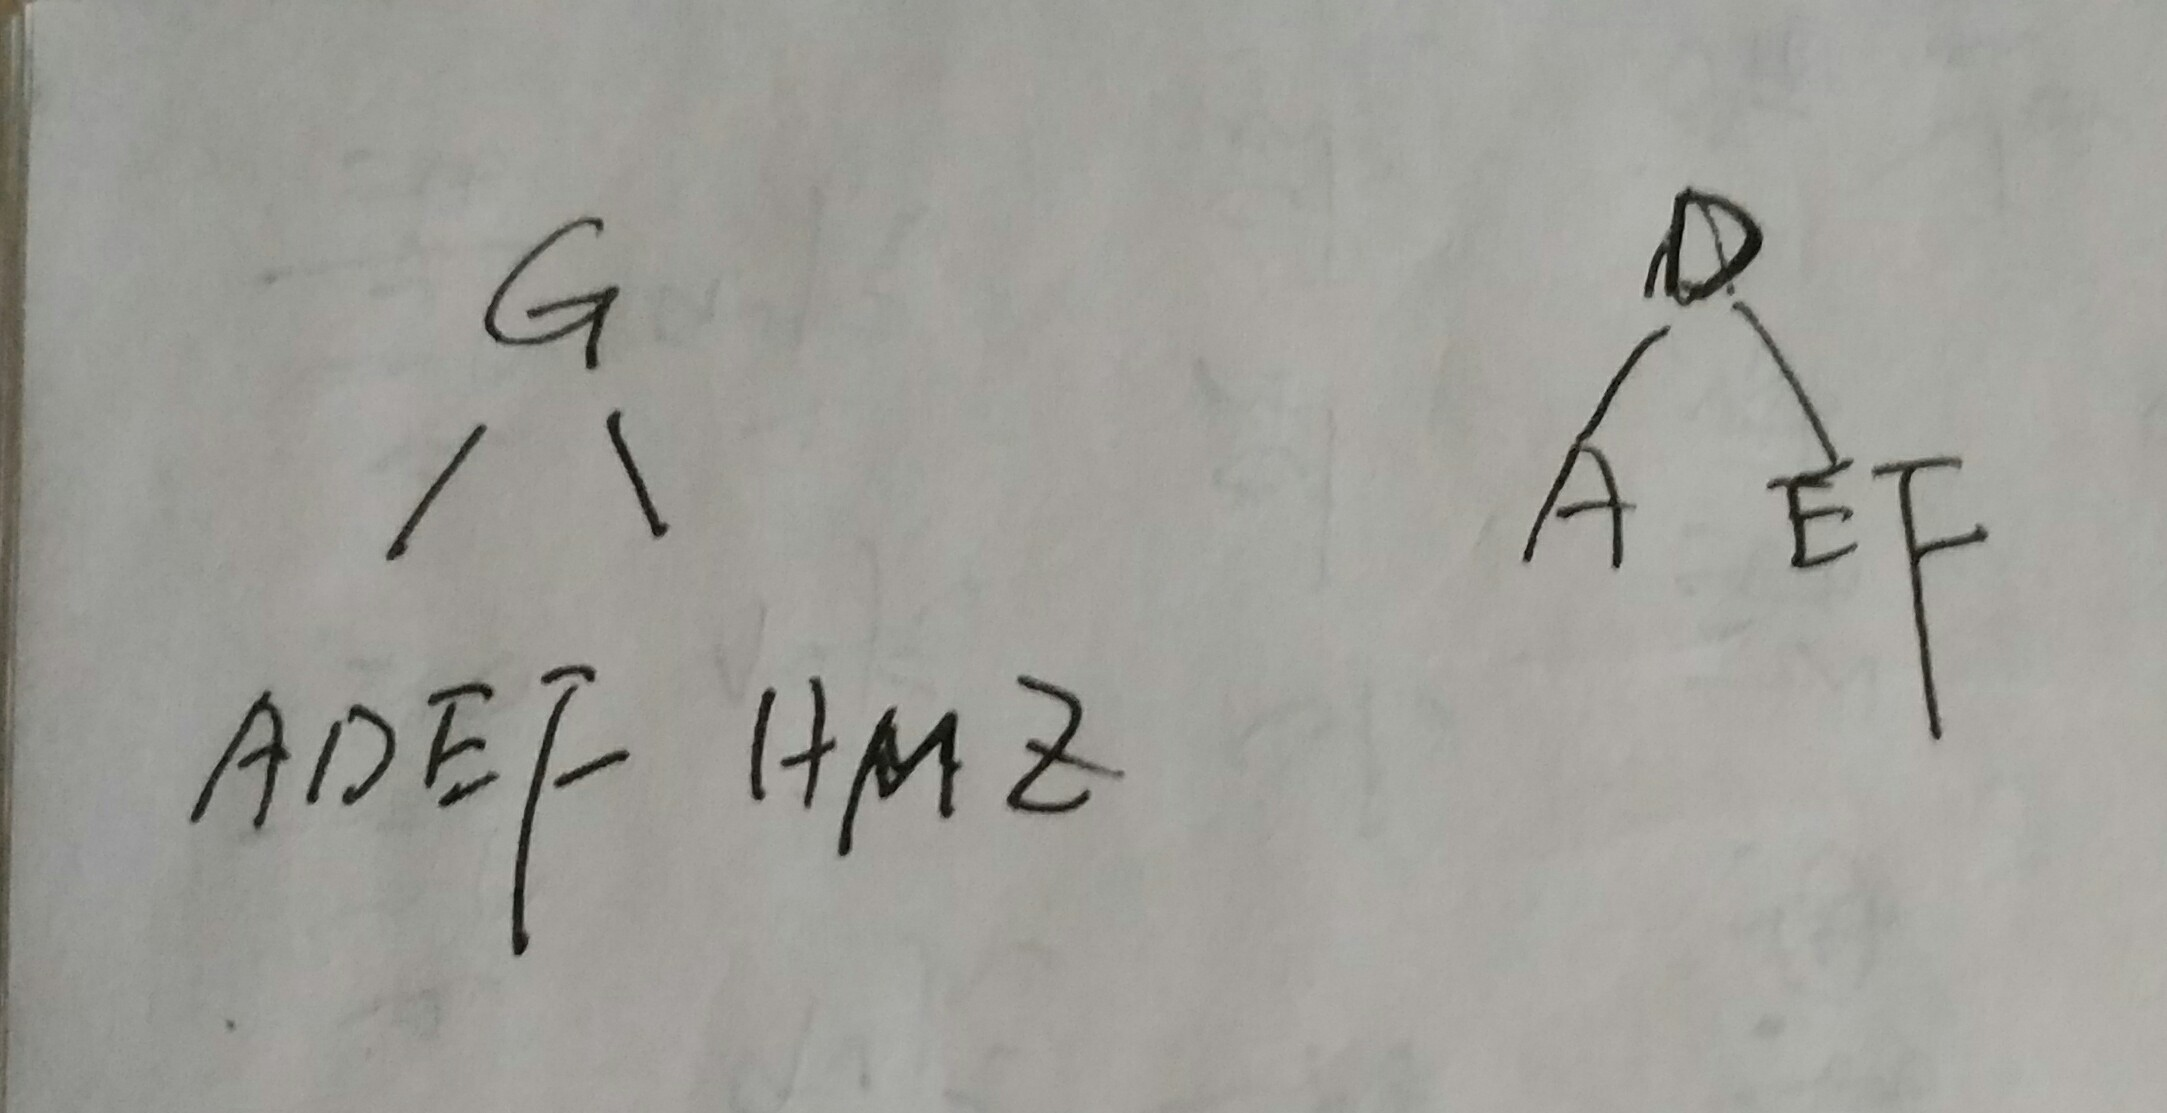
\includegraphics[width=.5\textwidth]{BinaryTreeTraversal}
\end{figure}

但还要找到对应的前序顺序。对左子树 ADEF 来说,在前序遍中的顺序
是 DAFE,说明左子树的根节点是 D, 从其中序顺序可知,左子树是 A, 右子
树是 EF. 重复此过程即可得出二叉树,再得出后序遍历 AEFDHZMG.

同理,已知后序遍历和中序遍历,也可求出前序遍历。唯一的区别是后序遍
历的最后一个节点是根节点,每次找根节点时从最后找。不管是哪种题,中
序遍历一定要有!

%%% Local Variables:
%%% mode: latex
%%% TeX-master: "main"
%%% End:

\chapter{栈}
\label{cha:algo-stack}

\section{进栈出栈}

栈是一种\uline{连续}据构,数据在栈内连续存储。栈有栈顶和栈底类似链
表的首部和尾部,区别是栈在垂直上下方向生长,链表在水平左右向生长。
如果需要,我们也可以用水平示意图表示栈,左边是栈底,往右生
长,如数组模拟栈就是这种思路。C/C++ 内存中的栈区即是一种栈结构。

给定一有 n 个元素的\uline{有序序列} $a_1, a_2, \cdots, a_n$, 对栈有
两种基本操作:\uline{进栈 push} 和\uline{出栈 out}. 无论是进栈还是
出栈,都是对栈顶进行操作。进栈也称压栈,表示保持元素间相对顺序把元
素存到栈顶,而出栈则表示取出栈顶的元素。

进栈、出栈组成一个\uline{动态操作序列},在 $n$ 个元素依次进栈的过程
中,伴随着元素随机出栈。动态操作序列有 $2n$ 个步骤,其中 $n$个
是进栈操作,另 $n$ 个是出栈操作。进出栈操作结束,栈为空,进栈的
$n$ 个元素亦全部出栈。

进栈顺序事先给定,用下标 $i$ 表示,表示为 $a_i,\; i \in
\{1,2,\cdots,n\}$. 出栈序列是进栈序列的某种排列,可记为
$a_{j_l},\; j_l \in \{1,2,\cdots,n\},\; l \in
\{1,2,\cdots,n\}$. $a_i$ 进栈操作和 $a_{j_l}$ 出栈操作\uline{相间
  出现}。$2n$ 个动态操作序列可记成:

\begin{align*}
  c_k,\; k \in \{1,2,\cdots,2n\},\; c_k\; \text{是}\; a_i\;
  \text{进栈或}\; a_{j_l}\; \text{出栈}
\end{align*}

可以肯定 $c_1$ 肯定代表 $a_1$ 进栈,$c_{2n}$ 表示某元素出栈。

实际上给定一个完整的出栈序列 $a_{j_l}$ 我们可以还原进出栈操作序列
$c_k$, 所以通常只需出栈序列 $a_{j_l}$ 即可。给出进栈序列 $a_i$ 在
$c_k$ 中的位置,我们可以推出剩下 n 个位置的出栈序列 $a_{j_l}$.

\section{先进后出}

进栈出栈遵循\textbf{先进后出,后进先出}的原则。对于\uline{当前栈内}元
素,后进栈的圧在先进栈的上边,栈顶永远是当前最后一个进栈元素,所以
先进栈的肯定比后进栈的后出栈,或说后进栈的肯定比选进栈的先出栈。换
句话说,任一时刻,栈的状态决定了当前栈内元素的相对出栈顺序。

总结起来,进出栈序列 $c_k$ 满足:
\begin{itemize}
\item $a_i$ 间的相对位置固定,因为进栈顺序事先给定。
\item $a_i$ 和 $a_{j_l}$ 符合先进后出。
\end{itemize}

可以看出,上面说的进栈出栈,不是指所有 n 个元素全部一次性入栈,再一
次性出栈。实际过程是进栈、出栈两种操作是交替进行,只要栈不为空,就
有可能进行出栈操作。如 $a_1, a_2$ 依次入栈(栈顶到底依次是 $a_2,
a_1$, 所以 $a_2$ 肯定比 $a_1$先出栈),接着 $a_2$ 立即出栈,$a_3$
入栈(栈内依次是 $a_3, a_1$,所以 $a_3$ 肯定比 $a_1$ 先出栈)。

前对对进出栈过程分析的比较清楚,任一时刻的栈内元素符合先进后
出原则。那么此原则是如何体现在完整操作序列 $c_k$ 里的呢?

\textbf{出栈序列里任一元素 $a_{j_l}$, 比其后出且先进的元素倒序。
  这些元素排在 $a_{j_l}$ 后面(后出栈),而且下标比 ${j_l}$ 小(先
  进栈)。它们(包括 $a_{j_l}$ 在内)一定是按下标降序排列}!

我们可以据此判断一个出栈序列是否正确。如 $3,4,5,1,2,9,8,7,6$ 是出栈
序列的下标 $j_l$, 显然这个出栈序列不正确,因为出现了 $3,1,2$. 存在
某个栈状态,$3$ 圧在 $1$ 和 $2$ 上面,栈内元素由上到下依次
是 $3,2,1$.

为了便于运算,我们一般用下标直接代替元素本身!在验证时,我们遍历
$j_l$, 从其开始,后面比其小的是否全部降序。由上例,$4,1,2$ 和
$5,1,2$ 都不合法。

\section{栈深度最小值}

给出出栈序列 $a_{j_l}$, 问栈深度最小值是多少。

在进出栈动态操作过程中,元素或进栈或出栈,栈内元素个数不定。栈需容
纳未出栈元素。如果每进栈一次,再出栈一次,则栈深度只需 1 即可。如
果所有元素全部入栈再出栈,则栈深度最少为 n.

对于一般情况,该如何算呢?其实很简单,只需利用上面的降序原则。遍历
出栈序列,对 $a_{j_l}$, 数出从其开始往后,降序元素个数(包含
$a_{j_l}$),最大值即为栈的最小深度。

\section{出栈序列数}

出栈序列数是指,给出进栈序列 $a_i$, 有多少种出栈序列 $a_{j_l}$?

操作序列 $c_k$ 有 2n 个位置,一旦确定了进栈序列 $a_i$ 的 n 个位置,
则立马得到出栈序列。也可以选出 n 个位置作为出栈序列,但是出栈序列内
部还有先后问题,所以用前一种思路更好。

从 $2n$ 个位置中选取 n 个的方法数是组合数 $C_{2n}^n$, 但进栈序列的
选位方法数比这小。如 $a_1$ 进栈肯定在第 1 位,而且 $a_i$ 肯定不能
排在最后 n 个位置。所以最终的方法数肯定是 $C_{2n}^n$ 除以或减去某
个数。

如果对进出栈计数,用 $+1$ 表示一次进栈,$-1$ 表示一次出栈,则任何时
候栈内元素个数就是这些 $\pm 1$ 的和。显然,任一时刻,栈内元素不能是
负数个,入栈次数肯定\uline{不少于}出栈次数,$+1$ 个不小于 $-1$ 个
数,$\pm 1$ 的和 $\geqq 0$.

对应到 $c_k,\; k \in \{1,2,\cdots,2n\}$ 序列,从头至尾扫描(水平示
意图),对 k 编历, 对任意 k, 前 k 个位置里,$+1$ 个数不少于 $-1$ 个
数。进出栈操作完毕,$n$ 个 $+1$ 和 $n$ 个 $-1$ 总和为 0. 有时为了方
便,直接用 $\pm$ 表示即可。有的地方用 $+1$ 和 $0$ 分别表示进栈、
出栈,最后的 $C_k$ 是一个二进制数。

总结起来是,\textbf{进出栈序列 $C_k$ 的所有前缀子串皆满足 $+1$ 个
  数不小于(大于等于) $-1$ 个数}。

特别地,当 $k = 1$ 时,前 1 位只能是 $a_1$ 进栈,和加 1 为 1. 当 $k
= 2n$ 时,最后 1 位是某元素出栈,和减 1 为 0.

所以我们要在 $C_{2n}^n$ 的基础上排除和为负的情况,也即在栈为空时或
为负时,进行出栈操作,也即在遍历 k 的过程中遇到和为负数情况。

假设在遍历 k 的过程中,第 1 次遇到和为 $-1$ 时,
有 m 个 $-1$, 则$+1$为 $m - 1$ 次,此时
$k = 2m - 1,\; m \in \{1,2,\cdots,n\}$. 显然 k是奇数,m 最大值
是 n. 特别地,第 k 位是 $-1$, 前面 $2m - 2$ 位中,分别有 $m -
1$ 位 $+1$ 和 $-1$. 后面 $2n-k$ 位里面有 $n - m +
1$ 个 $+1$, 剩下 $n - m$ 位是 $-1$.

对于奇数 k, 非法方法数是不是

\[
  C_{2m-2}^{m-1}C_{2n-(2m-1)}^{n-(m-1)} =
  C_{2m-2}^{m-1}C_{2n-(2m-1)}^{n-m}
\]

呢?此式表示前 $2m - 2$ 个位置里选 $m - 1$ 个出来放 $+1$ 表示进栈,
剩下的 $2n - (2m - 1)$ 个位置里选 $n - (m - 1)$ 个放剩下的
$+1$. 从 $-1$ 的角度分析,结果是
$C_{2m-2}^{m-1}C_{2n-(2m-1)}^{n-m}$. 答案是否定得!因为这种选取方
法不能保证前面 $k - 1$ 位里不出现和为负的情况。

我们可以换个思路。第 1 次遇到和为 $-1$ 时,后面 $2n-k$ 位的和
是$+1$,即进栈次数比出栈多 1. 如果交换后面的 $\pm 1$, 则可以得到一
个满射,组合计数不变。交换后面的 $\pm 1$ 后,$2n$ 位里面有 $n +
1$个 $-1$ 和 $n - 1$ 个 $+1$, 总和为 $-2$, 出栈比进栈多 2 次。反过
来,总和为 $-2$ 时总能找到第 1 次和为 -1 的情况。所以总的非法进出
栈方法数是 $C_{2n}^{n+1} = C_{2n}^{n-1}$, 那么合法进出栈总数为:

\begin{align*}
  C_{2n}^n - C_{2n}^{n+1} = \frac{C_{2n}^n}{n+1}
\end{align*}

这其实是一个卡特兰数~\ref{cha:catalan-number}.

至此,我们从组合数的角度直接得出进栈数序列数为卡特兰数。进出栈序操
作序列,对应对组合数学问题,是在 $2n$ 个位置上,选取 n 个放 $+1$ 或
$-1$, 要求是对位置 k 遍历,和为非负整数。

\section{进出栈递推方法}

下面我们从递推方法分析进出栈问题。分析算法问题时,我们可以找出问题
不同规模之间的联系,具体点就是递推关系。在算法领域,初始条件非常重
要。同一公递推公式的因为不同的初始条件而产生不同的数列。

用 f(n) 表示出栈序列数。先看进出栈的小规模问题。明显 $f(1) = 1$,
只有 1 个元素 $a_1$ 时,其进栈再出栈,只有一种可能。对于 $f(2) =
2$ 时:

\begin{enumerate}
\item 第一种是 $a_1$ 进,$a_1$ 出,$a_2$ 进,$a_2$ 出:$+-+-$
\item 第二种是 $a_1$ 进,$a_2$ 进,$a_2$ 出,$a_1$ 出:$++--$
\end{enumerate}

当 $n > 2$ 时,我们就要抽象分析了。分析有两个思路。第一种是考虑 n 个
元素里,哪个最先出栈,也即出栈序列里,谁是第 1 个元素。第二种是考虑
第 1 个元素 $a_1$ 出栈时所在位置,也即 $a_1$ 在出栈序列排第几位。我
们先看第一种思路。

\subsection{最先出栈元素}

如果是 $a_1$ 最先出栈,则出栈序列是 $a_1, a_{j_l},\; j_l \in
\{2,3,\cdots,n\}$. 很明显,$c_k$ 前两位是 $+-$, 表示 $a_1$ 进栈后立
马出栈。$a_1$ 进栈、出栈后不影响其后元素的进出栈,因为后面 $n - 1$
个元素根本还没入栈,这是一个 $n - 1$ 规模的子问题,有 $f(n - 1)$ 种
可能。

如果是 $a_2$ 最先出栈。此时其前元素 $a_1$ 已入栈并且没出栈。同
理 $a_2$ 最先出栈不影响后面元素 $a_i, i \in \{3,4,\cdots,n\}$ 的出栈序
列,因为后面元素根本还没入栈。其后元素有 $f(n - 2)$ 种可能出栈序列。
其前面的 $a_1$ 穿插于其后元素出栈序列之间。

对于一般情况,$a_k, k \in \{1,2,\cdots,n\}$ 最先出栈。此时
$a_i, i \in \{1,2,\cdots,k-1\}$ 已入栈并且没出栈。由前面分析可知,
这 $k - 1$ 个元素元素下标比 k 小(先进栈),但比 $a_k$ 后出栈,在出
栈序列里必须是(相对)降序排列(包括 $a_k$ 在内),即 $a_k,
a_{k-1},\cdots,a_1$. 因为在 $a_k$ 先出栈的条件下,从栈顶到栈底依次
是 $a_{k-1},a_{k-2},\cdots,a_1$. 特殊的,如果 $k = n$, 则 $a_n$ 最先
出栈,说是所有 n 个元素依次全部进栈,然后依次倒序出栈。

对于下标比 k 大的元素而言,$a_k$ 最先出栈不影响 $a_i, i \in
\{k+1,k+2,\cdots,n\}$ 出栈。后面元素的出栈是规模为 $n - k$ 的子问
题,有 $f(n - k)$ 种可能。

这个一般情况有多少种可能呢?考虑出栈序列
$a_k, a_{j_l},\; j_l \neq k, j_l \in \{1,2,\cdots,n\}$. 除了第 1
位 $a_k$, 余下 $n - 1$ 位里先选 $k - 1$ 个出来按序放 $a_{k-1},
a_{k-2}, \cdots, a_1$. 余下的 $n - k$ 位是 $a_i,\; i \in
\{k+1,k+2,\cdots,n\}$ 的出栈序列,对应序列数是 $f(n - k)$. 所以最
终是是:

\begin{align*}
C_{n-1}^{k-1}f(n-k) = C_{n-1}^{n-k}f(n-k),\; k \in \{1,2,\cdots,n\}
\end{align*}

为保证定义完备性,当 $k = n$ 时,我们定义 $f(n-n) = f(0) = 1$. 所
以 $a_i,\; i \in \{1,2,\cdots,n\}$ 的出栈序列数是:

\begin{align*}
  f(n) &= \sum_{k = 1}^nC_{n-1}^{n-k}f(n-k) = \sum_{k=1}^n C_{n-1}^{k-1}f(n-k) \\
  f(1) &= f(0) = 1
\end{align*}

\textbf{很可惜这个结果是错的}!乘法原理要求相乘的两个部分没有交集。
上面的分析里,保证了后面 $n - k$ 个元素的出栈相对序列,也保证了前
面 $k - 1$ 个元素倒序出栈,但当两个部分合在一起时,用乘法原理时,有
部分不符合要求。如 $a_k,a_{n-1},a_2,a_1,a_{n-3},\cdots$ 这个出栈序
列里,$a_k$ 前面的 $a_2,a_1$ 保持了降序,$a_k$ 后面
的$a_{n-1},a_{n-3}$ 是子问题,但是合在一起
时,$a_{n-1},a_2,a_1,a_{n-3}$ 这 4 个元素不是严格降序。

虽然这个分析错误,但能加强我们对进出栈问题的理解。

\subsection{$a_1$ 出栈位置}

下面从最先入栈的元素 $a_1$, 也即第 1 个元素出栈序号入手分析问题。
设 $a_1$ 第 $k,\; k \in \{1,2,\cdots,n\}$ 位出栈,则
在 $a_1$ 前有 $k - 1$ 个元素出栈,$a_1$ 后有 $n - k$ 个元素出栈。

可以肯定,$a_1$ 第 k 位出栈时,栈刚好为空,表明有 k 个元素入栈并完
全出栈。那么这 $k - 1$ 个元素是哪些呢?$a_1$ 第 1 位入栈后,有 $k
- 1$ 个元素先入进出栈,$a_1$ 等这些元素出栈后才最后出栈。明显这 $k
- 1$ 个元素就是 $a_i,\; i \in \{2,3,\cdots,k-1\}$.

假设 $a_l,\; k \leq l \leq n$ 在前 $k$ 个出栈元素中。
若 $a_l$ 在第 1 位出栈,据上一小节思路,这 k 个位置显然放不
下 $a_l, a_{l-1},\cdots,a_1$ 这 l个元素。若 $a_l$ 在第 2 位,
则 $a_l$ 和 $a_1$ 间的距离更短了,而且此时第 1 位是比 $a_l$ 更靠后
的元素了,同样容不下那么多元素。

以 $k = 2$ 为例, $a_1$ 出栈前要等 1 个元素先出栈。这个元素只能
是 $a_2$. 假假是 $a_3$, 则出栈序列是 $a_3,a_1,\cdots$, 显然中间
的 $a_2$ 没有正确出栈。从另一个角度看,$a_3$ 第 1 个出栈,这个序列
没有保证 $a_3,a_2,a_1$ 间相对降序出栈。因此 $a_1$ 等的不可能
是 $a_2$ 后的任何元素。

这 k 个元素的进出栈是一个完整的子问题,最先入栈的最后出栈。由于
第 k 位确定为 $a_1$, 则规模为 $k - 1$. 方法数是 $f(k - 1)$.

在 $a_1$ 后面进出栈的元素是 $a_i,\; i \in \{k+1,k+2,\cdots,n\}$ 这
$n - k$ 个元素。通过上面分析得,$a_1$ 在第 k 位出栈时,其前 $k -
1$ 个元素和后 $n - k$ 个元素的进出栈序列完全独立,互不影响。后面
$n - k$ 个元素的进出栈也是一个完整的子问题,规模为 $n - k$, 方法数
是 $f(n - k)$.

根据乘法原理,$a_1$ 第 k 位出栈时,方法数为 $f(k - 1)f(n - k)$. 由
此 n 个元素的进出栈方法数是:

\begin{align*}
  f(n) &= \sum_{k=1}^n f(k - 1)\,f(n - k) \\
  f(0) &= 1
\end{align*}

此公式就是卡特兰数~\ref{cha:catalan-number}~的递推公式。不像上节,
这节分析没有错误。两个子问题的进出栈序列集合交集为空,符合合乘法原
理。

不难发现,进出栈动态操作过程中,一旦栈为空,就得到一个规模更小的完
整子问题。进出栈问题,可以分成很多小的子问题,这此子问题问互不影响。
特别地,当出栈序列为 $a_1,a_2,\cdots,a_n$ 时,每一步出栈操作都定义
了一个子问题,规模为 1, 一共有 n 个子问题. 任意 k, $a_k$ 进栈再出栈
时栈为空,构成一个进出栈子问题。

前面分析中,在给出 $a_1$ 出栈得到两个子问题,刚好互逆,并集是进出栈序列的全集。
对这两个子问题,我们还可以分成规模更小的子问题。这是从已知结果前提
下,一个递归分解过程。

另外,在出栈序列里,若 $a_1$ 所在位置为 k, 可以肯定 $a_1$ 前的元素
必须是 $a_i,\; i \in \{2,3,\cdots,k-1\}$. 同理,$a_1$ 后的元素肯定
是 $a_i,\; i \in \{k+1,k+2,\cdots,n\}$. 如果出现超出此范围的元素,
则出栈序列非法。由此也可以快速排除一个非法的出栈序列。不过,这只是
进出栈序列的一个必要非充分条件,不能用来找出正确出栈序列。

\subsection{递归编程}

进出栈问题里,栈的状态可以由两个参数表示,特入栈元素(栈外)个数 n
和栈内元素个数 k, n 和 k 组成一个有序队 $(n,k)$, 我们用符
号 $f(n,k)$ 表示进出栈操作序列。下一步可以进栈 $f(n-1,k+1)$, 也可以
是出栈 $f(n,k-1)$. 显然 $k = 0$ 时不能出栈。

$f(n,0)$ 表示初始状态,$f(0,0)$ 表示操作结束。用此思路,我们可以用
递归函数 $f(n,k)$ 列出所有进出栈序列。

\section{进出栈总结}

\begin{enumerate}
\item 进出栈序列串,任意前缀子串满足 $+1$ 个数不小于 $-1$ 个数。
\item 出栈序列串,任意 k, 下标比 k 小的并排 $a_k$ 后的元素,其下标
  降序。
\item 出栈序列串,$a_1$ 出栈时,左边是 $a_i,\; i \in
  \{1,2,\cdots,k-1\}$ 子问题, 右边是 $a_i,\; i \in
  \{k+1,k+2,\cdots,n\}$ 子问题。
\item 进出栈动态过程中,每次栈为空时,得到一个子问题,所有子问题合
  并是总问题。
\end{enumerate}

%%% Local Variables:
%%% mode: latex
%%% TeX-master: "main"
%%% End:

\chapter{Regular Expression}
\label{cha:regular-expression}

To learn regular expression, read
[Quickstart](https://www.regular-expressions.info/quickstart.html)
first. Check the bit-by-bit
\href{https://www.regular-expressions.info/tutorial.html}{authoritative
  tutorial} for details. To test and check regular expressions, go
to \href{https://regex101.com}{regex101.com}.

Pay attention to the terms \uline{character class} \lstinline|[ ]|
and \uline{capture group} \lstinline|( )|. A character class match
\textit{one and only one} character. So \lstinline|a[1-9]| does
not match a single character \verb|a|.

In regular expression, a dot matches any character except visual
newline. A negated character class matches a newline instead like
\lstinline|[^a-z]|.
To avoid that, use \lstinline|[^a-z\r\n]|.

Regex is not intended for or good at \textit{inverse} search. But
we can mimic this behavior by \textit{lookaround} at
\href{https://www.regular-expressions.info/lookaround.html}{Lookahead
  and Lookbehind Zero-Length Assertions}. It is quite
\href{https://stackoverflow.com/q/406230}{useful} when we want to
exclude something when matching.

For example, if the command is \lstinline|grep|, use option
\lstinline|-P| to enable \uline{PCRE} engine. The code below
excludes entries of which the URI part does not contain
\textit{itunes-assets}.

\begin{lstlisting}
cclog hpc access 201902141200 201902151200 | \
grep -P -m2 'http://aod\.itunes\.apple\.com/(?!itunes-assets).*headers='
\end{lstlisting}

However, we can resort to \lstinline|-v| to do the same work.

\begin{lstlisting}
cclog hpc access 201902141200 201902151200 | \
grep -m2 'http://aod\.itunes\.apple\.com/.*headers=' \
grep -v 'itunes-assets'
\end{lstlisting}

So when to use \textit{lookahead} and when to use
\textit{lookbehind}? From my experience, if you don't want
to match something \textit{immediately} following a
\textit{literal string}, then use \textit{lookahead}. Similarly,
if you don't want to match something immediately preceding a
literal literal string, use \textit{lookbehind}.

Like \lstinline|^| and
\lstinline|$| (for start and end of \textit{string}),
\lstinline|\b| is also an anchor for start and end of
\textit{word} like \lstinline|\bhello\b|. It can be called as
\textit{boundary}. The counterpart \lstinline|\B| matches at every
position where \lstinline|\b| cannot match.

To match a valid IPv4 address, use:

\begin{lstlisting}
^((25[0-5]|2[0-4][0-9]|[01]?[0-9][0-9]?)\.){3}(25[0-5]|2[0-4][0-9]|[01]?[0-9][0-9]?)$
\end{lstlisting}

When using regular expression, many commands
(i.e. \lstinline|sed|) use forward slash \verb|/| as
delimiters. In such cases, forward slash should be escaped. You
can use another delimter (i.e. \verb|#|) to avoid escaping.

Most of the time, forward slash is
\href{https://serverfault.com/q/892905}{not special} and escaping
is \href{https://stackoverflow.com/q/6076229}{not required}.

Recall in C language, a variable matches
\lstinline|[A-Za-z_][A-Za-z_0-9]*|.

%%% Local Variables:
%%% mode: latex
%%% TeX-master: "main"
%%% End:


\part{Programming}
\chapter{Bash}
\label{cha:bash}

\lstset{language=bash}

\section{Contact}
\label{sec:bash-contact}

\begin{table}[!h]
  \centering
  \begin{tabular}[!h]{c}
    \toprule{}
    HU Zhan \\
    zhan.hu@chinacache.com \\
    \bottomrule
  \end{tabular}
  \caption{Contact}
\end{table}

\section{Stop List}
\label{sec:bash-stop-list}

\begin{itemize}
\item The \uline{NUL} byte is an ASCII \textit{control character}
  \lstinline|0x00| (binary \lstinline|00000000|) resembling
  \lstinline|\t \b|. It is a valid character occupying one byte in
  memory but not visible \lstinline|printf| can produce them with
  \lstinline|\0| in the format spec. GNU/BSD \lstinline|find| can
  terminate filenames with them (\lstinline|-print0|). Bash's
  \lstinline|read| can stop (delimit) on them with
  \lstinline|-d ''|.
\item 
  \href{https://www.gnu.org/software/bash/manual/bash.html}{Bash
    Manual}
\item
  \href{https://www.gnu.org/software/bash/manual/bash.html#Definitions}{Definitions}
\item \href{https://github.com/koalaman/shellcheck}{shellcheck}
\item Expansion \$: variable, paramter, command, pathname,
  arithmetic, history, brace
\item Substitution: process, command
\item \href{http://mywiki.wooledge.org/BashParser}{Bash Parser}
\item Quoting: escape character \textbackslash{}, single quotes,
  double quotes, ANSI-C Quoting
\item declare -p name
\item Term \textit{newline} refers to a \textit{visual} and
  \textit{electronical} new line, which is what is shown (a real
  new line) when Enter key is pressed.
\item Apart from builtins and functions, other (exernal) commands
  (i.e. \lstinline|find; awk| are executed in a
  sub-shell. \textit{pipeline} and process substitution
  also runs in a sub-shell. You see that, the shell script and
  commands within it run at different levels.
\item A sub-shell is an \textit{enhanced} sub-process, almost an
  identical copy of the parent shell process. They share the same
  variables, functions, \textit{export}, and even
  \lstinline|$$| equals to that of parent process. In other words,
  sub-shell inherits almost everything! From Bash 4.0 onward, the
  BASHPID is set the child process instead. However, variable
  assignments within sub-shell would not bring side effects to the
  parent process like
  \lstinline|var=1; (var=2; echo $var) ; echo $var|. Read more at
  \href{http://mywiki.wooledge.org/BashFAQ/024}{FAQ disappear}.
\item Use builtin \lstinline|PWD| variable instead of
  \lstinline|pwd| command.
\item
  \href{https://adamdrake.com/command-line-tools-can-be-235x-faster-than-your-hadoop-cluster.html}{Command-line
    Tools can be 235x Faster than your Hadoop Cluster}
\item Command \textit{option} and \textit{argument} are slightly
  different. Options are usually specified with a hyphen and a
  single character (i.e. \lstinline|grep -E|) that is defined by
  the command author. Arguments are generated by users like
  \lstinline|printf "hello, world"|.
\item \textit{filename} and \textit{pathname} are used
  interchangeably.
\item Some synonyms for globbing/glob (depending on the context in
  which it appears) are pattern matching, pattern expansion,
  filename expansion, wildcard and so on. Unquoted glob does
  filename expansion. Bash uses glob while \lstinline|awk|,
  \lstinline|sed|, and \lstinline|grep| use regular
  expression. Specially, for \lstinline|find|, strings passed to
  the \lstinline|-name| option are used as glob.
\item
  \href{https://www.regular-expressions.info/tutorial.html}{Regular
    expression}; Extended regular expression. \verb|!re !ere !bre|
\item Pattern matching; Extended pattern matching
  \lstinline|shopt -s extglob|. \verb|!pe|
\item \lstinline|echo "\n" ; printf "\n" ; printf '%s' $'\n'|. A
  literal backslash followed by a literal \verb|n|
  (\lstinline|\n|) within a double or single quoted string
  preserve their literal character meaning insteat of
  \textit{newline}. To print as a newline, use
  \lstinline|printf|. Whether \verb|\n| is treated as a newline
  depends on the context. To insert a lieteral newline, use
  \href{https://www.gnu.org/software/bash/manual/bash.html#ANSI_002dC-Quoting}{ANSI-C
    Quoting} \lstinline|$'foo\nbar'|.
\item \href{https://unix.stackexchange.com/q/32409}{set
    vs. shopt}.
\item In Bash man page, check \verb|Lists| for how Bash commands 
\end{itemize}

\section{Bash Parser}
\label{sec:bash-parser}

\href{http://mywiki.wooledge.org/BashParser}{Bash Parser} gives details
on how Bash processes script files or command lines, which helps
we understand the basic logic behind. Figure \ref{fig:bash-parser}
is a simplified image illustration.

\begin{figure}[!htb]
  \centering
  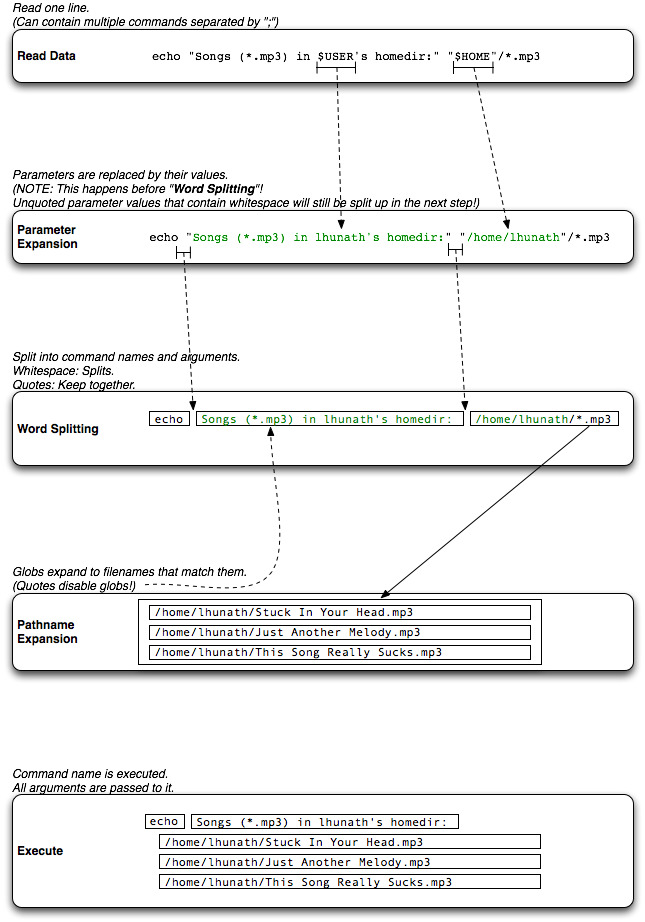
\includegraphics[width=.8\textwidth]{bash-parser}
  \caption{Bash Parser}
  \label{fig:bash-parser}
\end{figure}

Figure \ref{fig:bash-architecture} is a
\href{http://aosabook.org/en/bash.html}{better presentation}. From
which, we find \textit{expansion} plays a critical role in the
whole procedure.

\begin{figure}
  \centering
  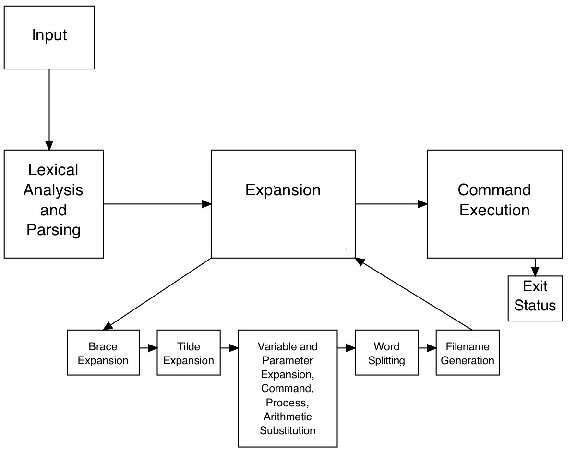
\includegraphics[width=.8\textwidth]{bash-architecture}
  \caption{Bash Architecture}
  \label{fig:bash-architecture}
\end{figure}

Basically, the parser carries out the following procedures:

\begin{enumerate}
\item Read script source line by line. For each line, 
\item Process quotes.
\item Split a line into commands. For each command,
\item Process redirections and brace expansions.
\item Perform expansions, including parameter expansion,
  comamnd/process/arithmetic substitution etc.
\item Word Splitting: split the command into command name and arguments list.
\item Execute the command.
\end{enumerate}

\section{Command History}
\label{sec:command-history}

Bash provides command-line tools for editing and manipulating
command history. Check the \uline{HISTORY EXPANSION} as per the
man
page. \href{https://samrowe.com/wordpress/advancing-in-the-bash-shell/}{Advancing
  in the Bash shell} is an excel tutorial.

One of the those is \lstinline|history|, listing previously
executed Bash commands. \lstinline|fc| is the counterpart for Sh
shell.

There exist a list of internal variables related to history
commands, like:

\begin{lstlisting}
$HISTCMD $HISTFILESIZE !N !-N !! !$ 
\end{lstlisting}

Especially, \lstinline|!!| is a synonym for
\lstinline|!-1|. \lstinline|!$| expands to the last word of the
preceding command. Usually, it will the the last argument.

Generally, we have \uline{Event Designator} that select a command
from history, \uline{Word Designator} that select a \textit{Bash
  word} from the selected command, and \uline{Modifiers} are a
sequence of modifiers to adjust the selected command. An event
designator starts with the exclamation mark \uline{!} .

One of the most useful modifier is \textit{p} that print but not
execute the selected command.

\section{Code Disassembling}
\label{sec:bash-code-disassembling}

I think it is a good practice to retrospect what have been learned
recently, reviewing progress and summarize
experience. Additionally, I'd like to make use of such chances to
format the knowledge in my own wording. Such an \textit{output}
process testifies whether knowledge settles down and consolidates.

This section disassembles the \verb|missTime| code line by
line. Especially, I should explain \textit{how} and
\textit{why}. The complete code is attached at
\ref{sec:bash-misstime}.

\section{Quoting}
\label{sec:bash-quoting}

Quoting is used to remove the special meaning of certain
characters (i.e. whitespace for word splitting) or words to the
shell. For example, it prevents reserved words from being
recognized as such. It can also prevent parameter expansion.

There exist multiple quoting mechanism, namely:

\begin{itemize}
\item the escape character \verb|\|
\item single quote
\item double quote
\item ANSI-C quote
\end{itemize}

A non-quoted \textbackslash{} preserves the literal meaning of the
next character, with the exception of newline. \verb|\newline| is
treated as a line continuation like

\begin{lstlisting}
echo \
'hello, world'

echo 'hello,
world'
\end{lstlisting}

For quotes, there is no need to append the trailing backslash. The
newline splits the string into two lines.

Single quotes preserve the literal meaning of each character
within the quotes, except single quote (even preceding by a
backslash which also preserves its literal meaning) like:

\begin{lstlisting}
echo 'what\'s your name?'
\end{lstlisting}

The backslash does not serves as escape. This is an illegal Bash
statement and it actually is parsed as three parts, namely
\lstinline|<what\>|, \lstinline|<s your name?>| and the final
apostrophe \verb|'|. The second part is not quoted and the third
single quote is unbalanced and Bash expects another single
quote. The revised versions are legal but may not be our desired
results.

\begin{lstlisting}
echo 'what\'s your name?
echo 'what\'s your name?'jim'
\end{lstlisting}

But if we \lstinline|printf '\n'|, a newline is correctly
printed. Why? That is because \verb|\n| is literally passed the
the command \verb|printf|. It is the responsibility of
\verb|printf| to interpret \verb|\n| as newline. For Bash, they
are just a backslash \verb|\| and character \verb|n|, not a
newline.

Apparently, single quotes is kind of \textit{strong} quoting
method to preserve character meaning. But we can precede it by
backslash \$ to preserve the escaping ability of \textbackslash{},
where escaped characters are replaced by their
\href{https://www.gnu.org/software/bash/manual/bash.html#ANSI_002dC-Quoting}{ANSI-C
  Quoting}. For example,
\lstinline|$'\t\''| presents a horizontal tab and a single quote
itself. Therefore, if we want to include a literal single quote
within singles qoutes, we can precede the quotes with dollar
\lstinline|$|.

Double qoutes is somewhat relatively flexible. It preserves the
literal meaning of all characters, except that of
\lstinline|$|, \lstinline|`|, \lstinline|\| etc. Within double
quotes, \textbackslash{} can be used to escape \lstinline|$|,
\lstinline|"|, \lstinline|`|, \lstinline|\| and
\verb|newline|. For example,

\begin{lstlisting}
echo "looooooooooooooooooooooooooooooooooooooooooooooooooooooooooooooooong\
,line. \$"

echo 'looooooooooooooooooooooooooooooooooooooooooooooooooooooooooooooooong\
,line. \$'
\end{lstlisting}

A double-quoted string preceded by a dollar sign
\lstinline|$"string"| will cause the string to be translated
according to the current \textit{locale}.  If the current locale
is C or POSIX, the dollar sign is ignored.  If the string is
translated and replaced, the replacement is
double-quoted. Attention, this is not parameter expansion, nor
ANSI-C quoting.

\section{printf and echo}
\label{sec:printf-echo}

\begin{lstlisting}
printf 'Usage: ./missTime <number-of-test> <input-file>\n\n'
\end{lstlisting}

Use Bash's built-in or system's \lstinline|printf| instead of
\lstinline|echo|. \lstinline|printf| supports all C language
format to allow flexible output. For instance, We can use it to
assign variables by \lstinline|-v| option:

\begin{lstlisting}
printf -v var "hello, world\n"; declare -p var
\end{lstlisting}

To check Bash's \lstinline|printf|, just run
\lstinline|help printf|. My Gentoo's system version is located at
\lstinline|/usr/bin/printf| that is part of GNU coreutils. In
terminal emulator, \lstinline|type -a printf| lists both
versions. Unlike \lstinline|echo|, \lstinline|printf| does not
append a \textit{newline} by default.

For the full contention, check
\href{https://unix.stackexchange.com/q/65803/74407}{Why is printf
  better than echo?} and
\href{https://wiki.bash-hackers.org/commands/builtin/echo}{echo
  protability considerations}.

As the page writes, \textit{never use options/arguments to echo}
like \verb|-e|. Also, do not use it to print \textit{uncontrolled
  data} such as external input (filename, arguments etc. from user).

In summary, \lstinline|printf| is far more reliable and safer. It
litterally output as the format specifies.

A final note, to output sequential dashes like \verb|---|,
\lstinline|printf| can do as follows:

\begin{lstlisting}
printf -- '---\n'
printf '%s\n' "---"
printf '---\n' # error
\end{lstlisting}

For the principle behind, just read Bash manual, the OPTIONS
section. Basically, everything after two consecutive dashes is
treated as arguments (i.e. filenames). In other words, it signals the
end of command options and disable further option processing.

Command \lstinline|tee -a| writes to both standard output and
files, which can be combined with \lstinline|printf| like:

\begin{lstlisting}
printf '%s\n' "hello, world" | tee -a file.txt
\end{lstlisting}

Single quotes are preferred in the format part unless you want
parameter expansion there.

Let's have a look at another sample:

\begin{lstlisting}
printf '%s\n' '1d' w | ed -s "$_full"

sed -i -e '1d' "$_full"
\end{lstlisting}

You will find there is only one format specification \verb|%s| but
two arguments \verb|'1d'| and \verb|w| (not quoted). In such case,
the format specifiers are reused:

\begin{quotation}
  The format is re-used as necessary to consume all of the
  arguments. If there are fewer arguments than the format
  requires, extra format specifications behave as if a zero value
  or null string, as appropriate, had been supplied.
\end{quotation}

\section{Exit Codes and Boolean}
\label{sec:exit-codes-boolean}

\begin{lstlisting}
[[ "$1" == @(-h|--help) ]] && exit 0
\end{lstlisting}

\lstinline|exit| terminates the current shell \textit{process}
while \lstinline|return| just terminates a \textit{function}
execution.

Both give numeric \verb|0| for success execution and other
specific codes for different error types. Here is a list of Bash
\href{http://tldp.org/LDP/abs/html/exitcodes.html#EXITCODESREF}{Reserved
  Exit Codes}.

The relation between Shell exit codes and boolean is as follows:
\textit{exit and return codes are just numeric integers}. They are
not boolean values. To be logically consistent, we should
correctly interpret the integer codes.

Bash treats 0 for true while others (1 included) for
false. Numeric 1 is just one instance among the whole set of
failure codes. It is not what we might think that false is bound
to 1. Let's have a closer look at the procedure.

A sub-shell decides the status of execution. If a desired
outcome is captured, it is logically true/successful. Otherwise,
different failure outcomes are treated as false.

Unpon successful execution, numeric 0 is returned back to the
parent process. Actually, any number could be returned to
represent
\href{https://stackoverflow.com/a/21439109/2336707}{successful
  execution}, but as the link points out 0 is \textit{platform and
  encoding independent}.

Now that numeric 0 is returned for success and other numerics for
failure, the caller or the topmost Bash process should correctly
interpret numeric codes to boolean true/false when \lstinline|if|,
\lstinline|[[ ]]|, or \lstinline|while| are involved.

Attention that, \textit{true} and \textit{false} are not
\href{https://www.gnu.org/software/bash/manual/html_node/Reserved-Word-Index.html}{reserved
  words} in Bash. But we have commands
\lstinline|type -a true false|. Up to now, you may find, many
commands has two versions: one from GNU coreutils and the other
from Bash builtins.

To test if a command is successfully executed, just test the command:

\begin{lstlisting}
if command ; then : ; fi
\end{lstlisting}

The next code also works, but it is \textit{stupid}. It runs a new
command \lstinline|[[| to test another command's exit code.

\begin{lstlisting}
# -or-
command; if [[ $? -eq 0 ]]; then : ; fi
\end{lstlisting}

Here, we find another command pair \lstinline|type -a [|.
\lstinline|[[| is only available to Bash.

\section{read}
\label{sec:bash-read}

\begin{lstlisting}
read -r _ _ _ _ip _ < <(ip -4 -o addr show scope global dev bond0)
 _ip="${_ip%/*}"
\end{lstlisting}

\lstinline|read| is another Bash builtin that read a line from
standard input and split it into fields based on \lstinline|IFS|
\begin{cprotect}
  \footnote{The default Internal Field Separator is <space>,
    <tabular>, and <newline>, namely \lstinline|$' \t\n'|.}
\end{cprotect}. Check details at
\href{https://www.gnu.org/software/bash/manual/bash.html#Word-Splitting}{Word
  Splitting}. You are recommended to include the \lstinline|-r|
argument as it disables bachslash escape.

\lstinline|read| assigns the first splitted word to the first
name, the second word to the second name and so on, with any
leftover words assigned to the last name.

Why are there \textit{underscore}s before and after
\lstinline|_ip|? Mainly, they are just placeholders to skip
unwanted splitted words, explained in the next section.

Thus, the first three undersocres capture the three words
ahead while the last underscore captures everything else, including the
IFS characters and leaving the remaining part untouched.

Attention that, \lstinline|read| uses \verb|IFS| as \textit{field}
separator while use \lstinline|-d| as \textit{record} separator.

\subsection{readonly}
\label{sec:bash-readonly}

The builtin \lstinline|readonly| command with the form

\begin{lstlisting}
readonly [-aAf] [name[=value] ...]

readonly -p
\end{lstlisting}

marks each \textit{name} as \textit{readonly}. if a \textit{value}
is supplied, do assignment before marking as read-only.

\section{Special Parameters}
\label{sec:bash-special-parameters}

These parameters may \textit{only be referenced}; assignment to
them is not allowed. Let's see how them are expanded.

\begin{itemize}
\item \verb|*|: \lstinline|$*| expands to positional
  parameter. Without double quotes, each positional parameter
  expands to a separate word. Within double quotes, all positional
  parameters expand to a single word with the value of each
  positional parameter separated by the first character of
  variable \lstinline|IFS|.
\item \verb|@|: \lstinline|$@| is similar to \lstinline|$*|,
  except that when in double quotes, each positional parameters
  also expand a separate word.
\item \verb|#|: \lstinline|$#| expands to the number of positional
  parameters in decimal.
\item \verb|?|: \lstinline|$?| expands to the exit status of the
  most recently executed \textit{foreground} pipeline.
\item \verb|-|: \lstinline|$-| expands to the current
  \textit{option} flags as specified upon invocation, by the
  \lstinline|set| builtin command, or those set by the shell
  itself (such as \lstinline|bash -i|).
\item \verb|$|: \lstinline|$$| expands the process ID of the
  \textit{topmost} shell. In a sub-shell (i.e. \lstinline|( )|, it
  expands the process ID of the invoking shell (upper level) as it
  is \textit{inherited}. In a sub-shell, use \lstinline|BASHPID|
  instead, which expands to the process ID of \textit{current}
  shell.
  \lstinline|echo $$ $BASHPID; ls -l /proc/self; (echo $$ $BASHPID; ls -l /proc/self)|.
  Also check
  \href{https://unix.stackexchange.com/a/333227}{/proc/self}.
\item \verb|!|: \lstinline|$!| expands to the process ID the
  \textit{job} most recently placed into the background.
\item \verb|0|: \lstinline|$0| expands to the name of shell or
  shell script.
\item \verb|_|: \lstinline|$_| expands to the last argument of
  privous simple command. Read the next section.
\end{itemize}

\section{Underscore}
\label{sec:bash-underscore}

Firstly, Bash regards \textit{underscore} \lstinline|_| as
\href{https://www.gnu.org/software/bash/manual/bash.html#Special-Parameters}{special
  parameter}. Meanwhile, it is a standalone legal \textit{name}
(vairable) and can be part of a variable as well. In short, it is
the \uline{only} \textit{parameter} that is also a valid
\textit{variable name}.

\begin{lstlisting}
echo 'hello, world'
declare -p _ ; declare -p _
\end{lstlisting}

As a special parameter, the value of undersocre \verb|_| is
assigned \textit{automatically} by Bash process as depicted in the
next section, namely \textit{expansion}
\ref{sec:bash-parameter-expansion}. At the very beginning, it is
set to the absolute \textit{pathname} of the shell or script
file. Subsequently, \textit{expand}s to the last argument of
previous simple command.

Though it is a variable, we can \textbf{not} assign value to it
explicitly. In other words, assignment to it is legal but in vain.

\begin{lstlisting}
_="a"
declare -p _
\end{lstlisting}

That is the reason we use it as a placeholder for \lstinline|read|
command. Its value is \textit{unstable} and got \textit{overriden}
immediately after each Bash command. Values assigned to it take no
effects. We can verify this behavior by:

\begin{lstlisting}
read -r _ var <<< 'hello, world'
declare -p _
# -or-
printf '%s\n' "$_"
\end{lstlisting}

The code outputs \lstinline|declare -- _="var"| since the last
argument of \lstinline|read| is a name (\verb|var| here).

Pay attention to the difference between \textit{declare} (only the
name is required) and \textit{printf} (name should be expanded by
\lstinline|$|).

\section{globstar}
\label{sec:bash-globstar}

The special glob character \lstinline|*| matches any string of any
length, including the \textit{null} string.

When the \lstinline|shopt -s globstar| option is enabled, two
ajacent two adjacent \lstinline|*|s used as a single pattern will
match all files and zero or more directories and subdirectories.
If followed by a \lstinline|/|, two adjacent \lstinline|*|s will
match only directories and subdirectories.

\textit{globstar} is also called \textit{recursive glob}.

\section{extglob}
\label{sec:bash-extglob}

Here are a few \textit{extglob} samples. To turn on this Bash
feature, just \lstinline|shopt -s extglob| \textit{on a newline}.

\lstinline|extglob| changes the way certain characters are
parsed. It is
\href{https://mywiki.wooledge.org/glob#extglob}{necessary to have
  a newline} (\textbf{not} just a semicolon) between
\lstinline|shopt -s extglob| and any subsequent commands to use
it. This is because the command line is parsed before
\lstinline|shopt| command is evaluated. Check the parser section
before.

Likewise, you cannot put \lstinline|shopt -s extglob| inside a
statement block that uses extended globs, because the block as a
whole must be parsed when it's defined; the \lstinline|shopt|
command won't take effect until the block is evaluated, at which
point it's too late. In fact as Bash parses the entire statement
block before evaluating any of it, you need to set
\textit{extglob} outside of the outermost block.

The first example below, does not turn on \lstinline|extglob|
correctly and report error.

\begin{minipage}{1.0\linewidth}
\begin{lstlisting}
shopt -u extglob
shopt -s extglob ; touch foo bar ; echo @(foo|bar)
# -bash: syntax error near unexpected token `('

_ip=127.0.0.1 _std_array[6]="https://www.baidu.com/a/b/c/d?v=k"
printf '%s\n' "${_std_array[6]}"
shopt -q extglob; _extglob_set=$?
(( _extglob_set )) && shopt -s extglob
_delete_url=${_reply_array[X-True-Cache-Key]#http?(s)://}
(( _extglob_set )) && shopt -u extglob

bash -c $'shopt -u extglob\nshopt -s extglob ; 
url="https://www.google.com/a/b/c" ;
_delete_url=${url#http?(s)://} ;
shopt -u extglob; printf "%s\n" "${_delete_url}"'

shopt -u extglob
var='--help' ; [[ "$var" == @(-h|--help) ]] && echo 'yes'
\end{lstlisting}  
\end{minipage}

The second case replaces the \lstinline|://host/| with
\lstinline|://ip/|, which combines the features of
\textit{extglob} and \textit{parameter expansion} in the form
\lstinline|${parameter/pattern/string}|. In the pattern part, we
should escape the backslash \textbackslash while in the string
part, leave as it is since this part is leterally substituted.

The next two cases show both
\lstinline|${parameter/pattern/string}| and \verb|[[| use
\lstinline|extglob| internally even we turn it off.

But to be consistent and robust, we are still recommended to put
it on separate lines. This rule applies to other shell options as
well.

\section{Process Substitution}
\label{sec:bash-process-substitution}

Still the same code snippet at previous section, we have

\begin{lstlisting}
< <(ip -4 -o addr show scope global dev bond0)
\end{lstlisting}

\lstinline|>(list)| and \lstinline|<(list)| are called
\href{https://www.gnu.org/software/bash/manual/bash.html#Process-Substitution}{Process
  Substitution} \textit{operator}s that allow a process's input or
output to be referred to using a \uline{filename}, which the
process get inputs from or output results to a file. Attention, a
sub-shell is spawned when process substitution happens (there is a
pair of parentheses there).

The keyword \textit{list} here may be a normal command or a
pipeline of commands. No space may appear between the \verb|<,>|
and the left parenthesis \verb|(|, otherwise the form would be
interpreted as a redirection.

The operators execute commands in \textit{list} in a sub-shell
and send the output to a file. The operator is then substituted
with the pathname of that file. Process Substitution is supported
on systems that support
\href{http://mywiki.wooledge.org/NamedPipes}{named pipes} (FIFOs)
or the \verb|/dev/fd/| method of naming opened files. We can just
think of the two forms as just filenames, which is done by giving
the list a name in the filesystem:

\begin{quotation}
  process substitution = filename
\end{quotation}

For the input form \lstinline|>(list)|, writing to the file will
provide input for the enclosed \textit{list} like:

\begin{lstlisting}
# command ... >(list) ...

echo >(true)

cat file.txt > >(wc -l)
\end{lstlisting}

The first example displays filename of the command
substitution. The second \textit{redirects} the output of
\lstinline|cat| to the input filename.

If the output form
\lstinline|<(list)| is used, the file can be read to obtain the
output of the \textit{list} like:

\begin{minipage}{1.0\linewidth}
\begin{lstlisting}
# command ... <(list) ...

echo <(true) # print the output filename
cat <(list)  # print the contents of the output filename

# compare the two output filenames
comm -3 <(sort a.txt | uniq) <(sort b.txt | uniq)
\end{lstlisting}
\end{minipage}

Back to the beginning code, the leftmost \verb|<| is a normal I/O
redirection, meaning read from the process substitution. Pay
attention to the extra space between the two \verb|<|, otherwise
it would be a
\href{https://www.gnu.org/software/bash/manual/bash.html#Here-Documents}{Here
  Document}.

\section{Parameter Expansion}
\label{sec:bash-parameter-expansion}

\begin{lstlisting}
_num_of_tests=${1:-10}
\end{lstlisting}

The purpose of this code is to assign value to
\verb|_num_of_tests| from either user input or the default
\verb|10|.

The special \$ symbol of Bash introduces \textit{parameter
  expansion}, \textit{command substitution}, or \textit{arithmetic
  expansion}. The terminology - \textit{parameter} - is defined in
the manul, please have a read. To put it simple, parameter is an
entity that stores values, it can be a \textit{name}, a
\textit{number}, or
\href{https://www.gnu.org/software/bash/manual/bash.html#Special-Parameters}{special
  parameters} like \verb|* @ # _| etc., of the list, undersocre is
explained in a prior section.

\textit{name} is what we usually call as \textit{varaible} or
\textit{function name}. Also referred to as an
\textit{identifier}.

The parameter symbol to be expanded may be enclosed in braces
which are \textit{optional} but \textit{safer} as braces separate
the variable from characters immediately following it.

The basic form is
\lstinline|${parameter}|. Our case is
\lstinline|${parameter:-word}| that means the expansion of
\textit{word} is substituted if \textit{parameter} is null or
unset, otherwise the value of \textit{parameter} is substituted.

Here are three extra examples:

\begin{minipage}{1.0\linewidth}
\begin{lstlisting}
for f in full real; do declare "_$f"="${_log_time}-${_num_of_tests}-$f.log"; done
for f in "${_full}" "${_real}"; do echo -n >| "$f"; done  
\end{lstlisting}
\end{minipage}

This code uses \lstinline|echo -n| to create an empty new
file, which can also be accomplished by \lstinline|touch| or
\lstinline|printf ''|

\section{Brace Expansion}
\label{sec:brace-expansion}

\href{https://wiki.bash-hackers.org/syntax/expansion/brace}{Brace
  expansion} is used to generate arbitrary \uline{strings}. It
takes the following forms:

\begin{lstlisting}
# {string1,string2,...,stringN}
{a,b,c,d}
# {<START>..<END>}
{1..10}
# {<START>..<END>..<INCR>} (Bash 4)
{1..10..2}
# <PREAMBLE>{........}
# {........}<POSTSCRIPT>
# <PREAMBLE>{........}<POSTSCRIPT>
a{b,c,d,}.txt
\end{lstlisting}

Both the PREAMBLE and POSTSCRIPT parts are optional. The last
example above can expand to \verb|a.txt| for the trailing
comma \lstinline|,|.

Within the braces, we can place either a series of comma-separated
strings, or a \textit{sequence expression}. The should be
\textit{no} space between the list elements. Results of expanded
strings are not sorted; let to right order is preserved.

A sequence expression takes the form \lstinline|{x..y[..incr]}|,
where \lstinline|x| and \lstinline|y| (both inclusive) are either
intergers or single characters, and \lstinline|incr|, an optional
argument, is an integer. Both \lstinline|x| and \lstinline|y| must
be of the same type.

Supplied integers may be prefixed with 0 to force each term to
have the same width like
\lstinline|for i in {01..12}; do echo $i; done|.

It is different to
\href{https://www.gnu.org/software/bash/manual/bash.html#Filename-Expansion}{globbing}
that matches \uline{filenames} by default (unless used in
parameter expansion).

\begin{quotation}
  This mechanism is similar to pathname expansion, but the filenames generated \textbf{need not exist}.
\end{quotation}

That means \lstinline|{foo,bar}.txt| expands to
\lstinline|foo.txt| and \lstinline|bar.txt|. Whether the two
strings are used as filenames or not depends on how you use it.

\begin{lstlisting}
for f in {foo,bar}.txt ; do echo "$f" ; ls "$f" ; done
\end{lstlisting}

But glob \lstinline|*.txt| only expands to \textit{existing} files. If
no files are matched, it expands to the glob itself unless
\lstinline|nullgob| is enabled which makes it expands to
\textit{null string}.

\begin{lstlisting}
bash -c $'shopt -u nullglob\nfor f in *.txt; do ls "$f"; done'

bash -c $'shopt -s nullglob\nfor f in *.txt; do ls "$f"; done'
\end{lstlisting}

From section Bash Parser \ref{sec:bash-parser}, we know brace
expansion happens before all the rest expansions. Any characters
special to other expansions are preserved in the result:
\textit{strictly textual}. So brace expansion makes

\lstinline|echo {a,b}$PATH|

be

\lstinline|echo a$PATH b$PATH|

before \verb|PATH| is parameter-expanded.

Similarly, a brace expansion with range like \lstinline|{1..200}|
can not be expressed like:

\begin{lstlisting}
a=1 b=200
echo {$a..$b}
\end{lstlisting}

Actually such code does not satisfy a legal barce expansion
requirement. Within the \textit{unquoted braces pair}, there
should be \textit{at least} a comma or a sequence expression.The
textual \verb|$a| and \verb|$b| (not parameter-expanded), the dots
inbetween included, neither contains a comma nor are sequence
expression. Hence, during the brace epxansion phase, the code is
ignored. When it comes to the parameter expansion, it becomes a
single string \lstinline|{1..200}|.

Brace construction is normaly used when the common prefix or
suffix of strings to be generated are much longer:

\begin{lstlisting}
mkdir /usr/local/src/bash/{old,new,dist,bugs}
#
chown root /usr/{ucb/{ex,edit},lib/{ex?.?*,how_ex}}
#
echo {{A..Z},{a..z}}
#
echo {A..Z}{0..9}
\end{lstlisting}

You will find from the code, brace expansion can be nested. It
also supports concatenation.

\section{Parameter Transformation}
\label{sec:bash-param-transf}

\begin{lstlisting}
printf 'curl -ksSI '
# 4.4
printf -- '-H %s ' "${_headers_array[@]@Q}"
printf -- '-H %s --resolve %s %s\n\n' "x-c3-debug:enabled" "${_resolve@Q}" "${_url@Q}"

# < 4.4
printf -- '-H %q ' "${_headers_array[@]}"
printf -- '-H %q --resolve %q %q\n\n' "x-c3-debug:enabled" "${_resolve}" "${_url}"
\end{lstlisting}

Since \href{http://mywiki.wooledge.org/BashFAQ/061}{Bash 4.4},
\uline{parameter transformation} is supported in the form
\lstinline|${parameter@operator}|. Of the operators, \verb|Q|
expands the parameter as a string that is the value of parameter
quoted in a format that can be reused as input like
\lstinline|ar=(a 1 "b ; c") ; printf '%s\n' "${ar[@]@Q}"|.

Before Bash 4.4, we can resort to \lstinline|printf '%q'| which
quotes the argument in a way that can be reused as shell input.

\section{regex Test}
\label{sec:bash-regex-test}

\begin{lstlisting}
_headers_regex=$'\^\~\$headers=\'(.*)\)@\|#\(\''
_headers_regex='\^\~\$headers='\''(.*)\)@\|#\('\'

_https_regex='^https://'
[[ "${_int_log}" =~ $_regex ]] && printf '%s\n' "${BASH_REMATCH[1]}"
\end{lstlisting}

Bash support the
\href{http://mywiki.wooledge.org/RegularExpression}{extended
  regular expression} by \textit{conditional command} \verb|[[|
with binary operator \verb|=~|.

If the pattern is properly matched, results is assigned to
built-in variable \lstinline|BASH_REMATCH|. It is an array
variable with index 0 the portion of the string matching the
entire regular expression (the complete match, \textbf{not} the
whole string). The element with index \textit{n} is the portion of
the string matching the \textit{n}th parenthesized sub-expression
(capture group). If there are nested parenthesis level, the inner
index is that of the outer level plus 1.

\lstinline|BASH_REMATCH| is \textit{read only}. We cannot change
its value. Usually, just assign it to a temporary variable.

Pay attention the two methods to define the regular
expression. The first one is preceded by a
\verb|$| within which \verb|\'| is correctly interpreted. While
the 2nd version, put the \verb|\'| outside of single
quotes\verb|'foo-bar'|.

\section{Array}
\label{sec:bash-array}

Bash provides one-dimentional \textit{indexed} and
\textit{associative} array variables. The \textit{declare} builtin
can explicitly declare an array:

\begin{lstlisting}
declare -a indexed_array # optional
declare -A associative_array=()
\end{lstlisting}

Indexed array can be any vairable, and hence a declaration is
optional.

\begin{quotation}
  Any reference to a variable using a valid subscript is legal,
  and bash will create an array if necessary.
\end{quotation}

On the contrary, associative array \textit{must} be
declared before usage.

Indexed arrays are zero-based while associative array resembles
Python \textit{dictionary}, with key and value pairs stored. Pairs
are not sorted.

When assigning elements to an array, please enfold the
\textit{subscript} with square brackets.

\begin{lstlisting}
indexed_array[0]=12
indexed_array=( [1]='a' 'b' 'c' )
printf '%s\n' "${indexed_array[@]}"
#
declare -A associative_array=( ['addr']='usa' )
associative_array['name']='jim'
associative_array=( ['age']=30 )
for key in "${!associative_array[@]}"; do printf '%s: %s\n' "$key" \
"${associative_array[$key]}"; done
\end{lstlisting}

Array elements can be referrenced by the form
\lstinline|${name[subscript]}|. The curly braces are required to
avoid conflicts with filename expansion operators.

\begin{quotation}
  \lstinline|${|. Without curly braces parameter expansions refer
    to the \textit{longest valid variable name} or
    \textit{shortest positional parameter}.
    \lstinline|"${var}bar"| expands the parameter named
    \textit{var} while \lstinline|"$varbar"| expands
    \textit{varbar}.
    \lstinline|"$123"| references \lstinline|argv[1]| and
    \lstinline|"${123}"| references \lstinline|argv[123]|. Braces
    are requried for positional parameters \uline{> 9},
    \uline{special PEs}, and \uline{array expansions}:
    \lstinline|${10}|, \lstinline|${var##pat}|,
    \lstinline|${arr[5]}|. BRACES AREN'T A SUBSTITUTE FOR QUOTES!
  \end{quotation}

If the \textit{subscript} is
omitted, \lstinline|$name| implies a subscript of zero \verb|0|,
which suggests \textit{name} is an indexed array or an associative
array with a key of zero \verb|0|.

\begin{lstlisting}
unset ar; declare -A ar=( [0]=a ["hello"]=1 )
declare -p ar; printf '%s\n' "$ar"
[[ -v ar ]] && echo "yes"
\end{lstlisting}

To print array:

\begin{lstlisting}
# indexed array
printf '%s\n' "${idexed_array[@]}"
# associative array
for key in "${!idexed_array[@]}"
do
    printf '%s: %s\n' "$key" "${idexed_array[$key]}"
done
\end{lstlisting}

The code above uses special subscript \lstinline|@| that expands
to positional parameter. Another special subscript is
\lstinline|*|, when double quoted, expanding to a single word with
each element separated by the first character of the
\lstinline|IFS| which by default is \textit{space}. Hence:

\begin{enumerate}
\item For printing, use \lstinline|@| instead of \lstinline|*|
  unless explicitly required.
\item When setting custom \lstinline|IFS|, pay attention to the
  character sequence.
\end{enumerate}

Now, let's have a look at the following code:

\begin{lstlisting}[caption={curl CRLF},label={lst:curl-crlf}]
declare -A _reply_array=()
while IFS=' :' read -r key value
do
    [[ -n "$key" && "$key" != [[:space:]] && "$key" != + ]] || continue
    _reply_array[${key,,}]=${value%$'\r'}
done < "curl-reply.log"
\end{lstlisting}

\begin{enumerate}
\item Associative array must be delcared.
\item The first character of \lstinline|IFS| is set to space.
\item \lstinline|-r| argument of \lstinline|read| is adopted.
\item \lstinline|continue| starts the next loop instantly.
\item \textit{key} is transferred to lower case by parameter
  expansion in the form
  \lstinline|${parameter,,pattern}|. \textit{pattern} is omitted.
\item Remove trailing \textit{carriage return} \lstinline|\r| from
  \lstinline|curl|.
\end{enumerate}

The sixth item is really hostile to programmers. Basically,
\lstinline|curl| feeds back messages with
\href{https://stackoverflow.com/a/30957952/2336707}{CRLF}
instead of \lstinline|\n|. We can check this by
\lstinline|sed -n l|. To reuse some returned headers, we should
firstly
\href{https://stackoverflow.com/a/35019553/2336707}{remove} the
extra \lstinline|\r|.

\section{Command Substitution}
\label{sec:bash-command-substitution}

Similar to Process Substitution
\ref{sec:bash-process-substitution} above,
\href{https://www.gnu.org/software/bash/manual/bash.html#Command-Substitution}{command
  substitution} performs the expansion by executing the command
within a sub-shell.

It allows the output of a command to substitute the command
itself, with trailing newlines delete. We can just think of
command substitution as a string and using the output of a command
as an argument. No filenames are involved.

It takes the following two
forms. The \textit{backquote} form is deprecated and discouraged.

\begin{lstlisting}
$(command)

`command` # deprecated
\end{lstlisting}

If the substitution appears within double quotes like
\lstinline|"$(command)"|, \textit{word splitting} and
\textit{filename expansion} are not performed on the results,
which is a \textit{preferred} method.

Command substitution is useful when we want to assign a command
output to a variable like \lstinline|_date="$(date -Idate)"|.

The command substitution \lstinline|$(cat file)| can be replaced
by the equivalent but faster
\lstinline|$(< file)| (without sub-shell). The later one is a
\textit{specical} case of command substitution. It does not invoke
any command and Bash just substitutes it with the contents of
file.

\section{Assignment and Simple Command}
\label{sec:assignm-simple-comm}

\begin{lstlisting}[basicstyle=\tiny\ttfamily]
IFS=$'\n' _log_array=( $( awk -F'[[:space:]]*\\)@(in|out)#\\([[:space:]]*' \
                              '{ for (i = 1; i <= NF; ++i) print $i; }' <<< "${line}" ) )
# better
mapfile -t _log_array < <( awk -F'[[:space:]]*\\)@(in|out)#\\([[:space:]]*' \
                              '{ for (i = 1; i <= NF; ++i) print $i; }' <<< "${line}" )
#
IFS=';' read -ra _headers_array <<< "${BASH_REMATCH[1]}"
_headers_array=( "${_headers_array[@]/#/-H}" )
\end{lstlisting}

In the first assignment uses \lstinline|awk| command substitution
with output assigned to an indexed array directly. This
substitution is not double-quoted, so word splitting and pathname
expansion happens before assignment. The second assignment uses
\lstinline|awk| process substitution and mapfile
\ref{sec:bash-mapfile} (explained in a standalone section), which
is much \textit{faster} and \textit{safer} method.

Why, in this section, I want to talk about assignment and simple
command? We can think of
\href{https://www.gnu.org/software/bash/manual/bash.html#Simple-Commands}{simple
  command} as just a command name followed by its arguments. From
\href{https://www.gnu.org/software/bash/manual/bash.html#Simple-Command-Expansion}{Simple
  Command Expansion}, we find:

\begin{quotation}
  If no command name results, the variable assignments affect the
  current shell environment. Otherwise, the variables are added to
  the environment of the executed command and do not affect the
  current shell environment. If any of the assignments attempts to
  assign a value to a readonly variable, an error occurs, and the
  command exits with a non-zero status.
\end{quotation}

The only command \lstinline|awk| is executed in a sub-shell, The
two assignments
\lstinline|IFS=$'\n' _log_array=| affect the current shell. That
is to say, from here on, the new \lstinline|IFS| value is changed
for the whole Bash process. Instead, the \lstinline|IFS|
associated with the \lstinline|read| statement only affects the
\lstinline|read| command itself.

Let's reformat the code like:

\begin{lstlisting}[basicstyle=\tiny\ttfamily]
IFS=$'\n'
_log_array=( $( awk -F'[[:space:]]*\\)@(in|out)#\\([[:space:]]*' \
                    '{ for (i = 1; i <= NF; ++i) print $i; }' <<< "${line}" ) )
IFS=$' \t\n'
\end{lstlisting}

It becomes more understandable and more clearer.

\paragraph{Extra notes}: \subparagraph{} Recall that indexed array
can be declared by \lstinline|-a| argument. \lstinline|read|
command supports reading into an indexed array by the same
argument.  \subparagraph{}
\lstinline|"${_headers_array[@]/#/-H}"| is another example of
parameter expansion in the form
\lstinline|${parameter/pattern/string}|. It inserts \lstinline|-H|
in front of each array element.

\section{Commands}
\label{sec:bash-commands}

\subsection{sed}
\label{sec:bash-sed}

\lstinline|sed|, as described in the manual, is a stream editor
for filtering and transforming text.

We can use it to delete empty lines:

\begin{lstlisting}
sed -i.bak '/^[[:space:]]*$/d' file.txt
sed -i.bak '/[^[:space:]]/!d' file.txt
\end{lstlisting}

The \lstinline|-i[SUFFIX]| or \lstinline|--in-place[=SUFFIX]|
option edits files in place (makes backup if SUFFIX supplied).

Form \lstinline|/regexp/| matches lines against the regular
expression. In the example above,
\lstinline|^[[:space:]]*$| matches empty lines. The traling
command \lstinline|d| means to delete matched lines.

To support extended regular expressions, add option
\lstinline|sed -r| like:
\lstinline|sed -r 's/[[:blank:]]+/ /g' /proc/slabinfo|. Otherwise,
the plus symbol should be escaped like:
\lstinline|sed 's/[[:blank:]]\+/ /g' /proc/slabinfo|.

The variant version is somewhat not so obvious but usually faster
if the file has less empty lines. Pay attention to the exclamation
mark \lstinline|!| before command \lstinline|d|. This version
means as long as a non-space character is matched, don't delete
the line.

Another useful form is \lstinline|s/regexp/replacement/| that
matches file lines agaist the \textit{regex} and \textit{replace}s
the matched parts with \textit{replacement}. We can use
\lstinline|&| in the \textit{replacement} to represents the
matched parts like \lstinline|s/hello/=&=/| means to enclose
string \textit{hello} with symbol \verb|=|.

The snippet below replaces \textit{google} with \textit{bing} if
the URL contains \textit{foo}. Note that in the regular expression
part, dot should be escaped while in the replacement part
\textit{not}. A version with \lstinline|awk| are also provided for
reference. Please read more in \verb|awk| section.

\begin{minipage}{1.0\linewidth}
\begin{lstlisting}
var=$'https://www.google.com/foo?v=xyz\nhttp://www.baidu.com/bar?v=uvw\n'
printf '%s\n' "$var"
sed '/foo/s/www\.google\.com/www.bing.com/' <<< "$var"

var=$'https://www.google.com/foo?v=xyz\nhttp://www.duckduckgo.com/bar?v=uvw\n'
printf '%s\n' "$var"
awk -F'/' 'BEGIN { ORS="/" } /foo/{ $3="www.bing.com" ; for ( i=1; i<=NF; i++ ) print $i }' <<< "$var"
\end{lstlisting}
\end{minipage}

In the meanwhile, special escapes \lstinline|\1| through
\lstinline|\9| refers to the corresponding matched sub-expressions
in the \textit{regexp}. To enable this feature, we should add
option \lstinline|-E| or \lstinline|-r|. For example,
\lstinline|-E s/(h.)l(.o)/\2/| will replace the word
\textit{hello} with \textit{lo}.

To match a continuous lines block, we have:

\begin{lstlisting}
sed -n '/addr1/,/addr2/p'
#
printf 'hello\nworld\nbash\nhello\nchina\n' | sed -n '/he/,/wo/p'
\end{lstlisting}

\begin{itemize}
\item the line which \uline{addr1} matched will always be
  accepted, even if \uline{addr2} selects an earlier line.
\item If \uline{addr2} is a \textit{regexp}, it will not be tested
  against the line that \uline{addr1} matched. In other words, if
  it is other forms (check man page, i.e. number), test is
  required.
\item If \uline{addr2} is not matched, all lines starting from
  \uline{addr1} to the end of file are matched.
\end{itemize}

Similarly, \lstinline|awk| has also such block address
feature. Check the relevant section below.

Here is an sophiscated example:

\begin{lstlisting}
~$ cat file
# Title: foobar
# Subject: Subject
# Body: Message body

# Title: foobaz
# Subject: Another Subject
# Body: Another message body

sed '/Title/,/Subject/s/foo/test/' file
\end{lstlisting}

Finally, to
\href{https://stackoverflow.com/q/12833714}{differentiate} the
concepts of \textit{pattern space} and \textit{hold space} is
important to master \lstinline|sed -n '1!G;h;$p'|.

\subsection{ed}
\label{sec:bash-ed}

\lstinline|ed| is \uline{line}-oriented text
editor. \lstinline|Sed| is a \uline{stream} editor.

A stream editor is used to perform basic text transformations on
an input stream (a file or input from a pipeline). While in some
ways similar to an editor which permits \textit{scripted} edits
(such as \lstinline{ed}), \lstinline|sed| works by making
\textbf{only one pass} over the input(s), and is consequently more
efficient. It is \lstinline|sed|'s ability to filter text in a
pipeline which particularly distinguishes it from other types of
editors.

Due to the \textit{stream} and \textit{one pass} features of
\lstinline|sed|, it cannot move back to earlier lines, where
\lstinline|ed| comes into usage.

\begin{lstlisting}
ed -s "${_full}" <<< $'$-3d\nw'
ed -s "${_full}" <<< $'$-3d\n,p'
\end{lstlisting}

\verb|$| refers to the last line and \lstinline|$-3| means the
last but 3rd line. Similar to \lstinline|sed|, command \verb|d|
means to delete the matched line.

Command \verb|w| means save the file. Usually \lstinline|ed|
allows only one command in a line except \verb|p|
etc. Consequently, we need \verb|\n| to separate \verb|d| and
\verb|w|. \lstinline|sed| on the other hand, allows semicolon
\lstinline|;| to separate different commands.

\subsection{awk}
\label{sec:bash-awk}

From the manual, \lstinline|awk| is a pattern scanning and
processing \textit{language}. You see! It is a programming
language, not just a command line tool.

There exist multiple \verb|awk|
\href{https://superuser.com/questions/75875/awk-mawk-nawk-gawk-what}{implementations},
of which \href{https://www.gnu.org/software/gawk/gawk.html}{gawk}
is, by default, deployed on all Linux distributions. This version
is the standard implementation for Linux, while the original
\verb|awk| was written for Unix v7. The original \verb|awk|
authors then released a new version called \verb|nawk| or
\verb|bawk| but rarely used. Another version is
\href{https://invisible-island.net/mawk/mawk.html}{mawk} that runs
\href{https://brenocon.com/blog/2009/09/dont-mawk-awk-the-fastest-and-most-elegant-big-data-munging-language/}{faster}
as it is based on a byte-code interpreter. On Linux systems,
\verb|awk| is a symbolic link to either \verb|gawk| or
\verb|mawk|. To
\href{https://stackoverflow.com/questions/33426591/awk-vs-nawk-vs-mawk-processing-heavy-files}{speed
  up} \verb|awk|, we can set \verb|LC_ALL=C awk 'foobar'|.

The basic form is as:

\begin{lstlisting}
gawk [ POSIX or GNU style options ] -f program-file [ -- ] file ...
gawk [ POSIX or GNU style options ] [ -- ] program-text file ...
\end{lstlisting}

\lstinline|awk| reads source code either from a external file or
from inline text.

We usually write \textit{program-text} like
\verb|pattern { action statements }|. Action statements (enclosed
in braces, \lstinline|{| and \lstinline|}|) will be performed on
the matched lines. Either the \textit{pattern} or \textit{action
  statements} part may be missing, but \textit{not} both. A
missing action is equivalent to \lstinline|{ print }|.

\textit{pattern} can be but not limited to \textit{/regular
  expression/}. The surrounding forwardslash is required like
\lstinline|awk '/[a-z][1-9]/ {print $1}'|. If the forwardslash is
omitted, \lstinline|awk| will treat it as a variable which usually
evaluates to null as it is probably undefined.

Another pattern is \textit{Relational expression} with operators
like \lstinline|+ - * / %| etc. It is
usually used to test whether certain fields match certain regular
expressions with \lstinline|~| or \lstinline|!~| like
\lstinline|awk '$4 ~ /^https/ {print $4}'|. Also, surround the
regular epxression with forwardslash.

However, a literal string (i.e. \texttt{http://}) with qoutes is
acceptable like \lstinline|awk '$4 ~ "^https:\\/\\/" {print $4}'|.
But we'd better use double backslash \textbackslash{} to
esecape special characters.

\lstinline|awk| also has \verb|BEGIN| and \verb|END| patterns
which are not tested against the input and can have their own
action statements. Actions defined in the \verb|BEGIN| are
performed before any input read while those of END are performed
when input is completely read.

We usually can change built-in variables in \verb|BEGIN| part like
\verb|FS RS OFS ORS|, where \verb|F| refers to \textit{field}
while \verb|R| means \textit{record}. Prefix \verb|O| for
\textit{print output}.

\begin{lstlisting}
awk 'BEGIN { print "Count \"hello\"" }
/hello/ { ++n }
END {print "\"hello\" appears in", n, "lines." }' file.txt

var=$'https://www.google.com/foo?v=xyz\nhttp://www.duckduckgo.com/bar?v=uvw\n'
awk 'BEGIN { FS=OFS="/" } $4~/^foo.*/ { $3="s3.bing.net" ; print }' <<< "$var"
\end{lstlisting}

For more details, refer to the PATTERNS AND ACTIONS section of the
manual.

Here is a real case:

\begin{lstlisting}
awk 'BEGIN {IGNORECASE=1}; /[-_]cache:/ { print substr($0, 3) }'
\end{lstlisting}

\lstinline|awk| accepts regular expression as \verb|FS| like
\ref{sec:bash-str-as-delim}. Here is a real case:

\begin{lstlisting}
gawk -F'\\^~\\$' '{ print $1 }' <<< '1^~$2'
mawk -F'\^~\$' '{ print $1 }' <<< '1^~$2'

awk 'BEGIN { FS="|" }; { print $2 }' <<< "abc|123"
\end{lstlisting}

Like \lstinline|sed|, \lstinline|awk| also accepts range pattern
\verb|pattern1, pattern2|. It matches all input records starting
with a record that matches \uline{pattern1}, and continuing until
a record that matches \uline{pattern2}, inclusive. It does not
combine with any other sort of pattern expression.

\begin{lstlisting}
awk '/pat1/,/pat2/'
#
printf 'hello world\nchina\n' | awk '/he/,/wo/'
printf 'hello world\nchina\n' | sed -n '/he/,/wo/p'
#
printf 'hello\nchina\n' | awk '/he/,/wo/'
\end{lstlisting}

If a record matches both patterns, then that single record is also
regarded as a range, which is slightly different from
\lstinline|sed|.

Attention that, \lstinline|awk| does not support \textit{lookeahd}
or \textit{lookahead} since it uses POSIX Extended Regular
Expression (ERE).

Check \href{https://stackoverflow.com/q/32481877}{What is NR==FNR
  in awk?}. Generally, \verb|NR| is the total number of records
(lines) read so far. \verb|FNR| is the line number (number of
lines) in the current file. Hence, \verb|FNR == NR| means
\verb|awk| is processing the first file as \verb|FNR| is reset to
1 for each new file.

Here is an interesting code:

\begin{lstlisting}
awk 'BEGIN { p = 0 }; tolower($0) ~ /keyword/ { p = !p ; next }; p' file.txt
awk 'tolower($0) ~ /keyword/ { p = !p ; next }; p' file.txt
\end{lstlisting}

It prints all lines after a line with 'keyword' (case-insensitive)
until a second line with 'keyword'. If there is only one line with
'keyword', the it prints lines until the end of file.

By default, variables are initialized to \verb|""| or \verb|0| if
not initialized by the \lstinline|BEGIN| pattern. Hence, the
\lstinline|BEGIN { p = 0 }| is optional. Variables defined by
\verb|-v| is better in that it accepts values from Shell like:

\begin{lstlisting}
awk -v var="$SHELL" 'BEGIN { print var }'
\end{lstlisting}

Then I want to talk about how \verb|awk| calls system commands:

\begin{itemize}
\item system(cmd-line)
\item cmd-line | getline
\end{itemize}

\verb|system()| may not be available on non-Posix
systems. Remember to close the opened command line as it has a
file descriptor associated.

\begin{lstlisting}
awk 'BEGIN { cmd="ls /"; system(cmd); close(cmd) }'
awk 'BGIN { cmd="ls /"; while(cmd|getline) print; close(cmd) }'
\end{lstlisting}

\subsubsection{grepawk}
\label{sec:grepawk}

\verb|!grepawk| writes:

\begin{lstlisting}
Awk can do almost everything grep can do. Instead of doing grep 'foo' | awk '{ statement }', try awk '/foo/{ statement }'
\end{lstlisting}

\subsection{grep}
\label{sec:bash-grep}

\lstinline|grep| print lines matching a regular expression
pattern. It has has two extensions, namely \lstinline|egrep| and
\lstinline|fgrep|. \lstinline|egrep| is equivalent to
\lstinline|grep -E|, while \lstinline|fgrep| is equivalent to
\lstinline|grep -F|.

\lstinline|egrep| uses the \textit{extended regular expression}
engine. Check the \uline{REGULAR EXPRESSIONS} section for
details. Specially, \lstinline|grep -P| uses PCRE engine (that of
Perl) which supports \textit{lookaround} as stated in a previous
section.

\lstinline|egrep| interprets pattern as an extended regular
expression while \lstinline|fgrep| interprets it as a list of
fixed strings separated by \textit{newline}s.

By default, it prints the matched lines. If we suppliy the
\lstinline|-v| option, not-matched lines are printed.

Another special option is \lstinline|-o| that prints only the
matched parts instead of the whole line.

\subsection{readline}
\label{sec:gnu-readline}

GNU
\href{https://www.gnu.org/software/bash/manual/bash.html#Command-Line-Editing}{Command
  Line Editing} is provided by
\href{https://tiswww.case.edu/php/chet/readline/rltop.html}{Readline
  Library} allowing users to edit command lines as they are typed
in. Both Emacs and Vi editing modes are available:

\begin{minipage}{1.0\linewidth}
\begin{lstlisting}
# enable
set -o emacs
set -o vi
# disable
set +o emacs
set +o vi
\end{lstlisting}
\end{minipage}

I am astonished that readline copies the key bindings from Emacs,
though it supports that of Vi editor. Table
\ref{tab:readline-bindings} lists some common key bindings:

\begin{table}[tbp]
  \centering
  \begin{tabular}{c|c}
    \hline{}
    Key Binding & Readline Function \\
    \verb|C-h| & DEL, Backspace \\
    \verb|C-_, C-x C-u, C-/| & undo \\
    \verb|C-l| & clear the screen, clear \\
    \verb|C-r| & backward search \\
    \verb|C-s| & forward search
  \end{tabular}
  \caption{Readline Key Bindings}
  \label{tab:readline-bindings}
\end{table}

If the terminal happens to turn on
\href{https://www.tldp.org/HOWTO/Text-Terminal-HOWTO-11.html}{Flow
  Control}, then \verb|C-s| will freeze your terminal. Use
\verb|C-q| to disable it.

\subsection{xargs}
\label{sec:gnu-xargs}

Compare the following two commands, we find that the first line
just prints \verb|--help| while the second prints the help message
of \lstinline|cat| command.

\begin{lstlisting}
echo '--help' | cat
# vs
echo '--help' | xargs cat
\end{lstlisting}

\lstinline|xargs| builds and executes \uline{command} from
standard input. It mainly reads items from standard input,
delimited by blanks and newlines, and pass the input to
\textit{command} as \uline{argument}s.

Actually, the idea is to concatenate a few items together and build
a new command to execute. It is sort of
\href{https://superuser.com/a/600273/221946}{converting STDIN
  contents to the command's arguments}, not passing the contents
to as input.

In the first example above, \lstinline|cat| uses STDIN as the
argument. And the conents of the argument is literl string
\verb|--help|. But in the second example, \lstinline|cat| uses the
contents of STDIN as its argument with the help from
\lstinline|xargs|. From this perspective, we find the necessity of
\lstinline|xargs| in spite of just \textit{pipeline}.

\lstinline|-d| option changes the default delimiters (blank and
newline) like \lstinline/echo '11@22@33' | xargs -d '@' echo/.

When building the new command, \lstinline|xargs| may encounter
filenames containing newlines or blanks which will broke the
results as the filename will be splitted.

This issue could be solved by passing \lstinline|-0| option to
\lstinline|xargs|, replacing the default delimiters to
\textit{null character} \lstinline|\000|.

Obviously, \lstinline|-0| option is equivalent to
\lstinline|-d'\0'|. This option is usually combined with
\lstinline/find ... -print0 | xargs -0 ... /. Check the
\textit{235x Faster} link in section \ref{sec:bash-stop-list} for
example.

By default, \lstinline|find| prints each found file followed by a
new line. But \lstinline|-print0| removes the newline:

\begin{lstlisting}
find . -type f -name *.txt -print | sed -n l
# ./test.log$
# ./sample.log$
find . -type f -name *.txt -print0 | sed -n l
# ./test.log\000./sample.log\000$
\end{lstlisting}

For safety, \lstinline|xargs| supports interactive execution by
\lstinline|-p|, prompting the user about whether to run the built
command.

Please further read
\href{https://www.cnblogs.com/wangqiguo/p/6464234.html}{xargs命令详
  解,xargs与管道的区别}.

\subsection{find}
\label{sec:bash-find}

\lstinline|find| is a powerful command, especially when followed
\lstinline|-exec| option. It usually takes the form:

\begin{lstlisting}
find [-H] [-L] [-P] [-D debugopts] [-Olevel] [starting-point...] [expression]
\end{lstlisting}

\lstinline|-H -L -P| control the treatment of symbolic links. The
\lstinline|-L| option follows symbolic links while \lstinline|-H|
does not follow symbolic links, except while processing the
command line arguments.

The term \textit{starting point} means a list of names of files or
directories to be examined. By default it is the current
directory, namely the single dot.

The \textit{expression} part is complicated. It is a kind of query
specification describing how we match files and what we do with
the files that were matched. An expression is composed of a
sequence of things:

\begin{lstlisting}
<POSITIONAL OPTIONS> <GLOBAL OPTIONS> <TESTS> <ACTIONS> <OPERATORS>
\end{lstlisting}

Check the relevant sections in the manual, to find out what they
are. Of the list, \uline{OPERATORS} join together the other items
within the expression. They include for example \lstinline|-o|
(meaning logical OR) and \lstinline|-a| (meaning logical
AND). Where an operator is missing, \lstinline|-a| is assumed.

Here are a few examples of \lstinline|find|:

\begin{lstlisting}
find -L /path/to/search -type f \( -iname "*filename*" -o -name '*.txt' \)

find -L /path/to/search -type f -iname '*.apk' -printf "%f\n" -exec cp -fv '{}' /path/to/copy \;

find APPs/ -maxdepth 1 -type f -iname '*.apk' -exec bash -c 'for file; do file="${file##*/}"; mkdir -p ROM/system/preset_apps/"${file%.apk}"; cp APPs/"${file}" ROM/system/preset_apps/"${file%.*}"; done' bash '{}' +
find -P history/ -type f -name '*.HEIC' -exec bash -c 'for file; do mv -v "$file" "${file%%.*}.heic"; done' 'bash' {} +
find ROM/system/media/wallpaper/ -depth -type f ! -path '*/wallpaper_15.png' -delete
find ROM/system/media/wallpaper/ -depth -type d -empty -delete

find -L . -type f -iname '*abc*' -exec bash -c 'mv "$0" "${0/abc/def}"' '{}' \;
export _pkg_name
find -H  -maxdepth 1 -type f \( -name '*.jpg' -o -name '*.png' \) -exec bash -c 'for img; do mv "$img" pics/"${_pkg_name}"; done' bash '{}' +
find . -type f -name '*.jpg' -exec bash -c 'for f; do mv $f ${f//"$0"}; done' $'\302\240' '{}' +
\end{lstlisting}

\begin{enumerate}
\item \lstinline|-name| and \lstinline|-iname| uses glob after
  \textit{word splitting}. It is recommended to quote the glob
  (explained below).
\item The surrounding parentheses force prededence of operators.
\item \lstinline|-type|, \lstinline|-iname|, and \lstinline|-name|
  are all \uline{TESTS}.
\item \lstinline|-printf| and \lstinline|-exec| are
  \uline{ACTIONS}.
\item \lstinline|-exec command ;| and
  \lstinline|-exec command {} +| are different. The first form
  executes the \textit{command} once for each file. The string
  special \verb|{}| is replaced by the current file name being
  processed. Both \verb|{}| and the semecolon \verb|;| may be
  quoted (i.e. \verb|'{}'|) or escaped (i.e. \verb|\;|) depending
  on the SHELL. The symbol \verb|{} +| appends each selected file
  name at the end and runs the the \textit{command} with all the
  files as arguments. The number of filenames is only limited by
  the system's maximum command line length. If the command exceeds
  this length, the command will be called multiple times. For
  example \lstinline|-exec ls {} +|. After the \verb|;| and
  \verb|+|, other \uline{ACTIONS} can be supplied.
\item \lstinline|-maxdepth| and \lstinline|-mindepth| are
  \uline{GLOBAL OPTIONS}.
\item \lstinline|-exec bash -c 'foo-bar' bash '{}' +|. The second
  literal string \textit{bash} serves as the
  \lstinline|$0| positional parameter to the Bash shell while
  \lstinline|'{}' +| serves as others. Without the second
  \textit{bash} string, the very first file name would be the zeroth
  positional parameter like
  \lstinline|-exec bash -c 'mv "$0" "${0/abc/def}"' '{}' \;|.
  This code will replace the \textit{abc} part of the zeroth
  positional parameter with \textit{def}. 
\end{enumerate}

From Bash manual, command \lstinline|for| takes the form:

\begin{lstlisting}
for name [ [ in [ word ... ] ] ; ] do list ; done
\end{lstlisting}

If the \textit{in word} part is omitted, \textit{name} expands to
the positional parameters.

The following two lines only differ whether a explicit \verb|0|
positional parameter is supplied. In the first case,
\lstinline|shift| makes \lstinline|for| to skipt the \textit{bash}
string. Otherwise, \textit{bash} would be processed as file name.

\begin{lstlisting}
-exec bash -c 'shift; for f; do foo-bar; done;' bash '{}' \;

-exec bash -c 'for f; do foo-bar; done;' '{}' \;

-exec bash -c 'shift; for f; do foo-bar; done;' '{}' \;
\end{lstlisting}

If \lstinline|-type d| \uline{TEST} is supplied, then probably the
\verb|0| positional parameter is the current directory, namely the
single dot. Sometimes we don't want to it to be processed within
\lstinline|for|. That is where the third case comes into
usage. Alternatively, we can use the \uline{GLOBAL OPTION}
\lstinline|-depth| which processes files within before the
directory itself.

Hence, some of the examples above should be rectified!

Now let's have a look at code:

\begin{lstlisting}
set -x

touch main.conf ; find . -type f -name main*
touch main.conf main1 ; find . -type f -name main*

touch main.conf main1 ; find . -type f -name 'main*'

set +x
\end{lstlisting}

Without quoting, \verb|main*| expands to filenames before passed
to \lstinline|find|. The second \lstinline|find| commands becomes

\begin{lstlisting}
find . -type f -name main.conf main1
\end{lstlisting}

That is an illegal command form. Hence the second example reports:

\begin{quotation}
  find: paths must precede expression: `main1'
  find: possible unquoted pattern after predicate `-name'?
\end{quotation}

So, always quote the glob after \lstinline|-name| option.

Another interesting point is how \lstinline|find| calculate
\textit{access} and \textit{modification} time. Take the option
\lstinline|$-mtime| for example, \lstinline|find| firstly
calcuates \textit{day}s passed since modification:

\[ ( \text{current-time} - \text{modification-time} ) / 86400 \]

The decimal fraction is \textit{rounded downwards} to the floor
like C language division. In a more fine-grained unit like
\textit{minute}, so the \uline{real modification age} is probably
greater than that. When option \lstinline|-mtime n| is used, files
of which the \textit{calculated modification age} is \textit{equal
  to} $n$ are matched. The real modification age of the matched
files belongs to $n$ to $n.\overline{9}$ days.

To strictly find out files whose calculated modification age is
greater than but not equal to $n$ days (\textit{at least} $n + 1$
days ago), we use \lstinline|-mtime +n|. On the contrary,
\lstinline|-mtime -n| requires the calculated age is less than but
not equal to $n$ (at most $n - 1$ days).

This rule also applies to other \textit{timestamp} options like
\lstinline|-atime, -ctime| etc. These options are all measured in
units of day, to get more accurate results, change to unit of
\textit{minute} like \lstinline|-amin, -cmin, -mmin|.

\lstinline|find| also supports comparing timestamp of two files
with \lstinline|-newer file, -newerXY file| where \uline{X} and
\uline{Y} are one of \uline{a B c m t}. For details, refer to the
'TESTS' section of the man page.

In addition to timestamp, we also have the
$\text{-size} \pm n[cwbkMG]$. Unlike the calculated timestamp, the
decimal fraction part of file size is \textit{rounded upwards} to
the next unit. So, when the unit is \uline{M}, a 1-byte file is
rounded up to \uline{1M}; if the unit is \uline{k}, then a 1-byte
file is rounded up to \uline{1k}. Take \lstinline|-size -1M| (less
than \lstinline|1M|) for example, the 1-byte file rounded to
\uline{1M} is not matched.

\uline{-1k} and \uline{-1M} \textit{only} match files of size
\textit{0}. To match a file size within $[0,1M]$, use \uline{-2M,
  -1025k}; \uline{1M} for $(0,1M]$; \uline{-1024k} for
$[0,1M)$. To avoid mistake introduced by different units, we can
stick to the byte unit \textit{c}.

Why file size is rounded up? By default, \lstinline|-size| uses
unit of \textit{512-byte block}. If a file size is 513 bytes, then
it would take 2 blocks.

In a nutshell, there exist two factors to consider when testing
timestamp or size, namely:

\begin{itemize}
\item the real timestamp/size versus the calculated ones;
\item option argument $[\pm] n$ denoting less than, equal to or
  greater than.
\end{itemize}

So to find a file modified at least 10 days ago and smaller than
1M, use:

\lstinline|find . -type f -mtime +9 -size -1024k|

\subsection{mapfile}
\label{sec:bash-mapfile}

\lstinline|mapfile| reads lines from the standard input into the
indexed array variable \textit{array}, or from file descriptor
\lstinline|FD| if the \lstinline|-u| option is supplied.  The
built-in variable \lstinline|MAPFILE| is the default array is no
array argument is supplied. It has a built-in synonym
\lstinline|readarray|.

\begin{minipage}{1.0\linewidth}
\begin{lstlisting}
mapfile -t _log_array < <( awk -F'[[:space:]]*\\)@(in|out)#\\([[:space:]]*' \
                               '{ for (i = 1; i <= NF; ++i) print $i; }' <<< "${line}" )
#
mapfile -t -d ';' _headers_array <<< "$var"
\end{lstlisting}
\end{minipage}

The \lstinline|-t| option removes trailing newline from from each
line input. \lstinline|-d| options can set a new delimiter than
the default newline.

Please read section \ref{sec:substr-as-delim} to find out how
\lstinline|while| loop achieves the same goal.

\subsection{time}
\label{sec:bash-time}

Before opening this section. I want to talk about a bit on
\href{https://www.gnu.org/software/bash/manual/bash.html#Compound-Commands}{Command
  Grouping}. Command grouping groups a list of commands to be
executed as a unit. It takes two forms:

\begin{lstlisting}
( list )

{ list; }
\end{lstlisting}

The parentheses executes commands of the \textit{list} in a
sub-shell environment. while curly braces executes them in current
shell.

\begin{itemize}
\item Especially, the trailing semicolon is required.
\item Curly braces are \textit{reserved words} of Bash. So they must be
  separated from the \textit{list} enclosed by by \textit{blank}s
  or other shell metacharacters.
\item Parentheses are \textit{operators}, and are recognized as
  separate tokens even they are not separated from the \textit{list}.
\end{itemize}

When commands are grouped, redirections may be
applied to the entire command list. For example, the output of all
the commands in the list may be redirected to a single
stream. This is how we capture the \textit{time} output.

\begin{lstlisting}
{ time curl -kLsSvo /dev/null "${_headers_array[@]}" \
            -H "x-c3-debug:enabled" --resolve "${_resolve}" "${_url}" 2>&1 | \
       awk 'BEGIN {IGNORECASE=1}; /<[[:space:]].*[-_]cache:/ { print
            substr($0, 3) }' ; } 2>&1 | tee -a "${_full}"

set -x; { echo foo; } 2> file; set +x; echo "file: $(< file)"
\end{lstlisting}

This section describes how to
\href{http://mywiki.wooledge.org/BashFAQ/032}{capture the time}
used for a command (into a file).

Script \lstinline|time cmd| prints the execution time of the
\textit{cmd} followed to \textit{time}'s \textit{stderr}, not that
of \textit{cmd}. We should tell apart the \textit{stdoud} and
\textit{stderr} of \lstinline|time| and \lstinline|cmd|.

Basically, we group the script with either \lstinline|{ }|
(preferred) or \lstinline|( )| (sub-shell). Within the group, we
capture output (\textit{stdout} and \textit{stderr}) of
\lstinline|cmd| while outside the group, we capture that of
\lstinline|time|.

The second case is \lstinline|set -x|. Similar to
\lstinline|time|, I want to capture the command executed into file.

\subsection{curl}
\label{sec:curl}

At the very first, I want to show the
\href{https://github.com/curl/curl}{curl}
\href{https://ec.haxx.se/cmdline-progressmeter.html}{PROGRESS
  METER} that shows downloading status in figure
\ref{fig:progress-meter-curl}.

\begin{figure}[tbp]
  \centering
  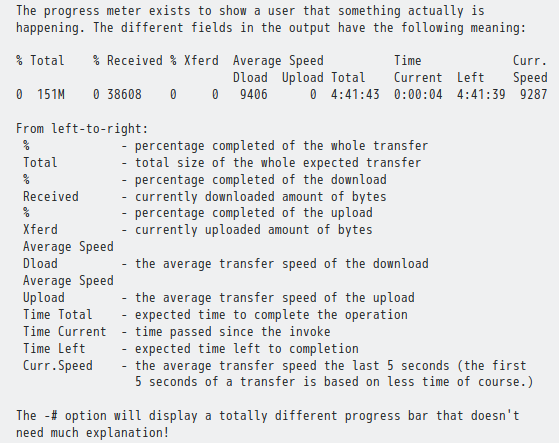
\includegraphics[scale=0.5]{curl-progress-meter}
  \caption{Progress Meter of curl}
  \label{fig:progress-meter-curl}
\end{figure}

To simplify the progress meter, \lstinline|curl| supports
\lstinline|-#| or \lstinline|--progress-bar| option.

Another useful option is \lstinline|-D| that dump the respond
headers to a file for later reference. Cookies from the respond
headers could be read by a second \lstinline|curl| invocation by
option \lstinline|-b, --cookie|. But pay attention to the
\uline{curl CRLF} issue \ref{lst:curl-crlf}. If followed by a dash
\lstinline|-D-|, headers will be dumped to STDOUT.

\subsubsection{curl POST PUT}
\label{sec:curl-post-put}

To post data to a remote server, firstly, we specify the HTTP
request method by \lstinline|-X POST| or
\lstinline|--request POST|. The data to be posted should be
specified by option \lstinline|-d, --data|. \lstinline|curl| will
send the data to the HTTP server in the same way a browser does
when a user has filled in an HTML form and press the submit
button. For example:

\begin{lstlisting}
curl -v -X POST --data 'name=jim' http://www.example.com/api/info
\end{lstlisting}

Data can be loaded from a file, which is done by
\lstinline|-d '@data.file'|. Attention that, the argument is
single-quoted:

\begin{lstlisting}
curl -v -X POST -d '@data.txt' http://223.202.75.26:32000/bm-app/apir/9120/qryLocationInfoAndIp

# data.txt:
name=jim&age=23
\end{lstlisting}

If \lstinline|-d '@-'| is used, then data is read from STDIN:

\begin{lstlisting}
curl -v -X POST -d '@-' http://223.202.75.26:32000/bm-app/apir/9120/qryLocationInfoAndIp
name=jim&age=23
^D
\end{lstlisting}

There are two common data formats, namely ``urlencoded'' and
``JSON'', taking the following two forms:

\begin{lstlisting}
-H "Content-Type: application/x-www-form-urlencoded"

-H "Content-Type: application/json"
\end{lstlisting}

Other formats like XML are not unusual as well. By default,
``urlencoded'' is used as it is concise and neatly organized. So
the ``Content-Type'' header can be omitted. Check this example:

\begin{lstlisting}
curl -v -X POST -H "Content-Type: application/x-www-form-urlencoded" -d 'name=jim&age=23' http://223.202.75.26:32000/bm-app/apir/9120/qryLocationInfoAndIp
\end{lstlisting}

For JSON data, it is recommended to load from external file:

\begin{lstlisting}
curl -v -X POST -H "Content-Type: application/json" -d '@api.json' http://223.202.75.26:32000/bm-app/apir/9120/qryLocationInfoAndIp

curl -v -X POST -H "Content-Type: application/json" -d '{"name": "jim", "age": 23}' http://223.202.75.26:32000/bm-app/apir/9120/qryLocationInfoAndIp
\end{lstlisting}

If the \lstinline|-d| option is supplied multiple times,
\lstinline|curl| will \textit{url-encode} the data before sending
out. \lstinline|--data 'name=jim' --data 'age=23'| will be merged
as \lstinline|'name=jim&age=23'|. It is quite handy for form
fields, though \lstinline|curl| supports option
\lstinline|-F, --form|.

The \lstinline|-d| option has multiple variants like
\lstinline|--data-raw|, \lstinline|--data-urlencode|,
\lstinline|--data-binary| etc. \lstinline|--data-urlencode| is
useful when if the data contain spaces like:

\begin{lstlisting}
curl -v -G "http://localhost:30001/data" --data-urlencode "msg=hello world" --data-urlencode "msg2=hello world2"

# /data?msg=hello%20world&msg2=hello%20world2
\end{lstlisting}

Read more in man page and check
\href{https://gist.github.com/subfuzion/08c5d85437d5d4f00e58}{curl.md}.

\subsection{wget}
\label{sec:wget}

Use \lstinline|wget| to download a remote directory with
\lstinline|-r, --recursive| option:

\begin{lstlisting}
wget -r -l2 -np -R "index.html*,mp3" -nH --cut-dirs=1 http://example.com/dir1/dir2/
\end{lstlisting}

\begin{itemize}
\item \lstinline|-l, --level| specifies the maximum recursion
  depth. By default, it is 5. Value \lstinline|inf| means
  \textit{infinite} recursion.
\item The \lstinline|-np, -no-parent| option does not ever ascend
  to the parent directory when retrieving recursively.
\item An \textit{intex.html} is automatically generated, which can
  be disabled by option \lstinline|-R, --reject| which rejects
  files by \textit{suffix} or \textit{filename}s if wildcard
  characters \lstinline|* ? [ ]| are used. For example,
  \lstinline|-R pdf| excludes PDF files while \lstinline|temp*|
  excludes filenames with leading string \textit{temp}.
\item By default, invoking Wget with
  \lstinline|-r http://fly.srk.fer.hr/| will create a local
  directory beginning with the host
  \textit{fly.srk.fer.hr/}. Option
  \lstinline|-nH, --no-host-directories| removes that.
\item \item \lstinline|--cut-dirs=number| ignores \textit{number}
  directory prefixes.
\end{itemize}

In the example above, \lstinline|-nH, --cut-dirs=1| creates a
local directory \textit{dir2/} without leading
\textit{fly.srk.fer.hr/dir1/} pathname. If we change
\textit{number} to 2, then all files are downloaded in current
directory < \uline{.} >

A similar option is \lstinline|-m, --mirror| to mirror a site. It
is equivalent to \lstinline|-r -N -l inf --no-remove-listing|.

\begin{lstlisting}
wget -m -np -nH --cut-dirs=0 -Epk -R "index.html*,mp3" -X "/video-dir/sexy" [--restrict-file-names=nocontrol] http://192.168.0.105:8080/a/
\end{lstlisting}

\begin{itemize}
\item \lstinline|-E, --adjust-extension| appends suffix
  \textit{.html} to \verb|application/xhtml+xml| or
  \verb|text/html| filenames if it does not end with
  \textit{regex} \lstinline|\.[Hh][Tt][Mm][Ll]?|.
\item \lstinline|-p, --page-requisites| downloads linked resources
  to display a given HTML.
\item \lstinline|-k, --convert-links| converts the links in the
  document to make them suitable for local offline viewing.
\item \lstinline|-X| is to reject unwanted directories, similar to
  \lstinline|-R, --reject|. Please use the full pathname
  \textit{relative} to the URL. \lstinline|-X "/video-dir/sexy"|
  means to exlude
  \textit{http://192.168.0.105:8080/a/video-dir/sexy}. The
  leading forwardslash is optional.
\item \lstinline|--restrict-file-names=nocontrol|. The term
  \textit{restrict} means to allow only characters of filename
  valid and safe to your local operating system. Invalid filename
  characters (including those unprintable control characters) are
  \textit{escaped}. Argument \textit{unix} would escape
  forwardslash \lstinline|/| and unprintable control
  characters. The argument \textit{nocontrol} tells Wget
  \textit{not} to escape control characters. It solves Chinese
  mojibak issue as parts of which fall into the range of control
  characters.
\end{itemize}

\paragraph{Re-downloading of the same pathname} By default,
downloading multiple copies of the same pathname would result in
new copies ending with number suffixes like \textit{pathname.1},
\textit{pathname.2} etc., which is called
\uline{clobbered}. Option \verb|-r| would \uline{overwrite} the
old copy with new one from server. Option \verb|-nc, --no-clobber|
just refuses to download any new copies and \uline{preserve} the
old copy. When option \verb|-N, --timestamping| is used, whether or
not to download a new copy depends on the local and remote
timestamp and size of the file. Remember, do not specify
\verb|-no| and \verb|-N| concurrently. Therefore, either
\verb|-r -nc| or \verb|-r -N|.

\paragraph{To use proxy} \lstinline|wget| supports \lstinline|-e|
option like \lstinline|wget -e https-proxy=127.0.0.1:8080|. Of
course, the proxy setting could set put in \lstinline|/etc/wgetrc|
or \lstinline|~/.wgetrc| like:

\begin{lstlisting}
use_proxy=on

http-proxy=127.0.0.1:8080
https-proxy=127.0.0.1:8080
ftp-proxy=127.0.0.1:8080
\end{lstlisting}

To turn off all proxies, set \lstinline|use_proxy| as
\textit{off}.

\subsection{rsync}
\label{sec:rsync}

We can use \lstinline|rsync| to synchronize files between a source
and a destination. Specially, if one end is an remote host,
\lstinline|rsync| can transfer data over \textit{remote shell}
(\href{https://serverfault.com/q/378939}{default} to
\lstinline|ssh|) or \textit{rsync daemon} (directly over TCP).

If the host is followed by one single colon, \lstinline|ssh|
connection is used. The option \lstinline|-e, --rsh=COMMAND|
specifies the remote shell to use. If it is two colons
(i.e. \lstinline|foo::|) or \lstinline|rsync://|, \textit{rsync
  daemon} is used.

\begin{lstlisting}
# -e "ssh" is optional
# -z compresses contents before transmission, usually used over
# network transmission
rsync -avzP -e "ssh" ~/workspace/src/ dev:~/dev/

# customize SSH port
rsync -avzP -e "ssh -p 2222" ~/workspace/src/ dev:~/dev/

# -n, --dry-run
rsync -n -avzP ~/workspace/src/ dev:~/dev/

# --delete to mirror the source and dest
# If a source file is deleted from the source, then delete it from
# the dest either. By default, only append.
rsync -avzP --delete ~/workspace/src/ dev:~/dev/
\end{lstlisting}

We cannot emphasize too much the paramount importance of trailing
forwardslash \verb|/|:

\begin{itemize}
\item If \verb|/| is placed at the end of the source folder,
  \verb|rsync| will copy the contents of the folder.
\item If the source folder is not followed by \verb|/|,
  \lstinline|rsync| will copy both the folder and contents
  therein.
\item If \verb|/| is palced at the end of the target folder,
  \lstinline|rsync| will paste the data directly inside that
  folder.
\item If the target folder is not followed by \verb|/|,
  \lstinline|rsync| will create the target folder and then paste
  the data inside.
\end{itemize}

\subsection{tr}
\label{sec:bash-tr}

Command \lstinline|tr| translates, squeezes, \uline{and/or}
deletes characters from standard input, writing to standard
output. It takes form as:

\begin{lstlisting}
tr [OPTION]... SET1 [SET2]
\end{lstlisting}

\uline{SET1} and/or \uline{SET2} define ordered sets of characters
like \lstinline|[:alpha:]| and \lstinline|c-g| (without
brackets). The format of the SET1 and SET2 arguments resembles the
format of regular expressions \ref{cha:regular-expression};
however, they are not regular expressions, only lists of
characters.

The \lstinline|-c -C --complement| option replaces SET1 with its
complement (all of the characters that are not in SET1). Currently
\lstinline|tr| fully supports only single-byte characters. So
characters like Unicode Chinese are not supported.

\textit{translate} means to substitute each character of its input
that is in SET1 to the \textit{corresponding} character in SET2
(required). Therefore, we usually want the lengths of both sets
are equal.

To replace comma with newline \lstinline|tr ',' '\n' < file|. It
is quite handy though we can do that with \lstinline|sed| or
\lstinline|awk|.

A common use of \lstinline|tr| is to convert lowercase characters to
uppercase.

\begin{lstlisting}
tr abcdefghijklmnopqrstuvwxyz ABCDEFGHIJKLMNOPQRSTUVWXYZ

tr a-z A-Z # discouraged method

tr '[:lower:]' '[:upper:]'
\end{lstlisting}

The bare range \verb|a-z| and \verb|A-Z| are discouraged as it is
not portable and depends on implementation.

Option \lstinline|-d| deletes characters in \uline{SET1} and do
\textbf{not} \textit{translate}. For example
\lstinline|tr -d '\0'| removes all zero bytes.

\lstinline|-s| can be treated as a special case of \lstinline|-d|,
which \textit{squeeze}s repeated occurence. For example,
\lstinline|tr -s '\n'| merge multiple blank lines to a single one.

Let's have a look at:

\begin{lstlisting}
tr -d -axM # fail

tr -d -- -axM
tr -d axM-
tr -d '[=-=]axM'
\end{lstlisting}

The code want to delete four characters in which hyphen is
included. In the first case, \lstinline|-a| will be treated as
command-line option. The last method uses \textit{equivalence
  class}. For details, check the \lstinline|info tr| page.

\subsection{dig}
\label{sec:bash-dig}

The \lstinline|+trace| option traverses the resolution system in a
\textit{iterative} resolution method. At the very first, local
name server (i.e. \textit{/etc/resolv.conf} is used to obtain a
list of root domain name server unless \lstinline|@name-server| is
specified. For example:

\begin{lstlisting}
# dig +trace www.bing.com. @1.2.4.8
\end{lstlisting}

\section{Math}
\label{sec:bash-math}

\href{http://mywiki.wooledge.org/ArithmeticExpression}{Arithmetic}
in Bash is \textit{integer} math only. To do floating point math,
resort to \textit{bc} command.

We call a \textit{math form} as \textit{math context}. The basic
math form is
\lstinline|$(())| with the complete syntax at
\href{https://wiki.bash-hackers.org/syntax/arith_expr}{arith expr},
which is called \uline{Arithmetic Expansion}. Basically, within a
math context, we use the same syntax as C language like.

\begin{minipage}{1.0\linewidth}
\begin{lstlisting}
# POSIX sh
i=$((j + 3))
lvcreate -L "$((24 * 1024))" -n lv99 vg99
q=$((29 / 6)) r=$((29 % 6))
if test "$((a%4))" = 0; then ...
echo "$((2**3))"
\end{lstlisting}
\end{minipage}

Within a math context, pay attention to the concept of the
\textit{evaluation value} of each \textit{arithmetic expression}
and the value returned to the Bash environment by the context
itself (name it \uline{context value}?).

\begin{itemize}
\item All C arithmetic operators are supported, including
  \verb|?:|. Bash brings in \textit{exponentiation} operator
  \verb|**|.
\item Within a single math context, multiple expressions can be
  separated by \textit{comma}. Value of the last expression
  becomes that of the math context.
\item Variable \textit{name} in a math context are substituted
  with their values (unset or empty variables are evaluated as
  0). There is no need to use parameter expansion
  (i.e. \verb|${i}|) within math context.
\item Numbers without leading 0 are treated as base 10. Numbers
  with a leading 0x are treated as base 16. Numbers with a leading
  0 (not followed by x) are treated as base 8.
\end{itemize}

\subsection{Arithmetic Command}
\label{sec:bash-arithmetic-command}

Besides, Bash offers two extra forms of math context by
\textit{commands} for which, the math context \textit{also} gets
an exit status, and side effects. Similar to arithmetic expression
\lstinline|$(())|, the context value of an arithmetic command is
that of the command exit code.

Exit code of arithmetic command \uline{depends on but not equal
  to} evaluation value of the last expression. If the
expression evaluates to 0 and the command is considered a falure. To
be logically consistent with Bash, the command returns 1
. Otherwise, the command is regarded successful and return
0.

Consequently,

\begin{itemize}
\item Evaluation and boolean logic (0 false, non-zero true) of
  math expressions are in accord with C syntax.
\item Exit code and boolean logic (0 true, non-zero false) of math
  commands are in accord with Bash.
\item Return eithr 0 or 1. Nothing else. This is different to the
  Arithmetic Expansion above. So we can the Arithmetic Command as
  a \lstinline|test| with \lstinline|for| or \lstinline|while|.
\item Please go back and read Exit Codes and Boolean
  \ref{sec:exit-codes-boolean}.
\item Whatever numeric values are involved, boolean logic must be
  guaranteed. This is the rule that we follow when
  scripting. Forget about the details then. Check
  \href{https://wiki.bash-hackers.org/syntax/arith_expr#arithmetic_expressions_and_return_codes}{Arithmetic
    expressions and return codes}.
\end{itemize}

The first arithmetic command is \lstinline|let|:

\begin{minipage}{1.0\linewidth}
\begin{lstlisting}
let a=17+23
echo "a = $a"        # Prints a = 40
#
let a=17 a+=23 a=0   # the last expression evaluates to 0
echo $?              # 1 (false)
#
let a[1]=1+1         # Wrong (if a1=1+1 exists or shopt -s failglob)
( shopt -s failglob; let a[1]=1+1 )
touch a1=1+1; let a[1]=1+1; declare -p a
let 'a[1]=1+1'       # right
\end{lstlisting}
\end{minipage}

Note that each arithmetic expression has to be passed as a single
argument to the \lstinline|let| command, so you need quotes if
there are spaces or globbing characters.

\lstinline/let a[1]=1+1/ is not right as \lstinline|[ ]| are
\href{http://mywiki.wooledge.org/glob}{glob} characters, which
matches one and only one of the enclosed characters like regular
expression.

\begin{quotation}
  Bash expands globs which appear \textit{unquoted} in commands,
  by matching \textit{filenames} relative to the current
  directory. The expansion of the glob results in 1 or more words
  (0 or more, if certain options are set), and those words
  (filenames) are used in the command.
\end{quotation}

So Bash tries to expand \lstinline|a[1]=1+1| as filename
\textit{a1=1+1} before \lstinline|let| is executed. If that file
exists or \textit{failglob} is turned on, Bash reports:

\begin{quotation}
  bash: no match: a[1]=1+1
\end{quotation}

Now let's move on to the next arithmetic command
\lstinline|(( ))|. It resembles Arithmetic Expansion but removes
the leading dollar
\lstinline|$| sign. It is identical to \lstinline|let| but does
not require quotes since expressions inside are delimited by
Bash metacharacters \lstinline|(| and \lstinline|)|.

\begin{lstlisting}
((a=$a+7))         # Add 7 to a
((a = a + 7))      # Add 7 to a.  Identical to the previous command.
((a += 7))         # Add 7 to a.  Identical to the previous command.

((a = RANDOM % 10 + 1))     # Choose a random number from 1 to 10.
echo $?                     # % is modulus, as in C.

echo "$(( a = RANDOM % 10 + 1 ))" # becomes Arithmetic Expansion
\end{lstlisting}

Specially, we can compare integers with
\lstinline|(())|. \lstinline|>| or \lstinline|<| inside
\lstinline|(( ))| means greater/less than, not output/input
redirection involved. Recall that I have talked about expression
evaluation and context exit code above. Integer comparision
expression also follows the same rules.

The only difference is that arithmetic expression within the
command is logic operation: only evaluates to 1 or 0. If the
comparison is true (command executes successfully), the expression
evalutes to 1 and returns 0. If it is false, the expression
evaluates to 0 and returns 1.

\lstinline|(( ))| is used more widely than \lstinline|let|,
because it fits so well into an \lstinline|if| or
\lstinline|while| command like

\begin{lstlisting}
if (( $# > 2 )) ; then printf 'there are more than 2 arguments\n'; fi
\end{lstlisting}

\subsection{bc calculator}
\label{sec:bc-calculator}

To do \href{http://mywiki.wooledge.org/BashFAQ/022}{floating point
  calculation}, we use \lstinline|bc|. However, by default, it
truncates according to the \textit{scale} argument instead of
rounding.

We increase \lstinline|scale| and pass the result to
\lstinline|xargs printf| like:

\begin{lstlisting}
bc <<< 'scale=3; 7/242.906' # 0.028
bc <<< 'scale=2; 7/242.906' # 0.02

bc <<< 'scale=3; 7/242.906' | xargs printf "%.2f\n" # 0.03
\end{lstlisting}

Another possible workaround is to use \verb|±0.5| trick with the final
result like:

\begin{lstlisting}
rounding()
{
    if (( $(bc <<< "$1 < 0") )) ; then offset=-0.5 ; else offset=0.5; fi
    printf "%.$2f\n" "$( bc -l <<< 'scale=$2; (((10^$2)*$1)+$offset)/(10^$2)' )"
    printf '%.*f\n' "$2" "$( bc -l <<< 'scale=$2; (((10^$2)*$1)+$offset)/(10^$2)' )"
}
\end{lstlisting}

Within the rounding function, we should set the offset according
to the sign of the number. If the number is negative, we choose to
round it toward the left side of number line. Or we can say to
round toward its absolute value. Of course, if we want to always
round toward the right side, then just use \verb|0.5|.

About \lstinline|printf '%.*f\n' "$2"|, the asterisk means the width
is given as argument
\href{https://wiki.bash-hackers.org/commands/builtin/printf?s\%5b\%5d=printf}{before}
the string or number is printed.

\section{Redirection}
\label{sec:bash-redirection}

Redirection takes the form as \verb|lhs op rhs|, which can
\textit{open}, \textit{duplicate}, \textit{move} or we want to
\textit{close} file descriptors.

\begin{itemize}
\item \textit{lhs} is always a file descriptor, namely an integer
  like \verb|0|, \verb|1|, \verb|2|, or \verb|3|. If the
  \textit{op} is \verb|<| then there is an \textit{implicit}
  \verb|0| as \verb|0<|. If it's \verb|>| or \verb|>>|, there is
  an \textit{implicit} \verb|1| as \verb|1>| or \verb|1>>|.
\item \textit{op} is \verb|<|, \verb|>|, \verb|>>|, \verb/>|/, or
  \verb|<>|. Two special redirections \verb|<<| (here document)
  and \verb|<<<| (here string) usually require string(s) for
  \textit{rhs}. Details, read the official manual.
\item \textit{rhs} is the thing that the file descriptor will
  describe. It can be a filename, or the place where another
  descriptor goes ( prefixed with \verb|&| like \lstinline|&1|),
  or \lstinline|&-| that will close the \textit{lhs} file
  descriptor.
\end{itemize}

When redirection is used, the \textit{lhs} is pointed to what
\textit{rhs} is \textbf{currently} pointed to. If, later on,
\textit{rhs} is pointed to another place, \textit{lhs} remains and
won't follow \textit{rhs}'s update. We can think of a file
descriptor as C language pointer.

To check which place file descriptors are currently pointed, we
can:

\begin{lstlisting}
ll /proc/$$/fd/

# total 0
# dr-x------ 2 outsinre outsinre  0 Feb 14 15:49 .
# dr-xr-xr-x 9 outsinre outsinre  0 Feb 14 15:49 ..
# lrwx------ 1 outsinre outsinre 64 Feb 14 15:49 0 -> /dev/pts/2
# lrwx------ 1 outsinre outsinre 64 Feb 14 15:49 1 -> /dev/pts/2
# lrwx------ 1 outsinre outsinre 64 Feb 14 15:49 2 -> /dev/pts/2
# lrwx------ 1 outsinre outsinre 64 Feb 14 21:10 255 -> /dev/pts/2

for fd in 0 1 2 255; do cat /proc/$$/fdinfo/$fd; echo; done
\end{lstlisting}

In the following code, \textit{cmd} reads input from filename
\textit{myFile}. File descripted \verb|3| is associated with
\verb|1| (standard output, \textit{/dev/pts/2}). But the script
does not make use of the new descriptor. \verb|2| (standard error,
\textit{/dev/pts/2}) is redirected to
\lstinline|/dev/null|. Standard output (implicit \verb|1|,
\textit{/dev/pts/2}) is redirected to \verb|2|, which is now
pointed to \textit{/dev/null}.

\begin{lstlisting}
# Good! This is clearly a simple commmand with two arguments and 4 redirections
cmd arg1 arg2 <myFile 3<&1 2>/dev/null >&2
\end{lstlisting}

There are two special redirection forms \lstinline|fd1>&fd2| and
\lstinline|fd1<&fd2|. As mentioned earlier, if \textit{fd1} is
omitted, the default value are \verb|1| and \verb|0|
respectivelly.

They are called \textit{descriptor copy} or \textit{descriptor
  duplication}. Technically speaking, the two forms \textbf{make no
  difference}. Yeah, they are equal in Bash grammar except the
different implicity \textit{lhs}.

\textit{fd1} is opened (created) if it does not exist, and pointed
to where \textit{fd2} is currently pointed. Whether \textit{fd1}
is opened for reading or writing, depends on \textit{fd2}. If the
file \textit{fd2} linked with is on read mode, then we can use
\textit{fd1} for reading. Similarly, we can write to \textit{fd1}
when \textit{fd2} points to a file on write mode. Obviously, if
the file is on read/write mode, \textit{fd1} can be used to read
from and write to that file.

In a script, we can do like this:

\begin{lstlisting}
exec m>&n
exec m<&n
# -or-
cmd arg1 arg2 m>&n
cmd arg1 arg2 m<&n
\end{lstlisting}

It is necessary to tell apart \verb|>, <| and \verb|>&, <&| as the
\verb|&| requires an integer descriptor followed while the former
needs a filename. More importantly, \verb|>, <| cares about the
read and write mode. \verb|>| opens a file descriptor for writing
(\uline{redirecting output}). The other one for reading
(\uline{redirecting input}). Apparently, \verb|>>| is for
\uline{appending redirected output}.

To open a file descriptor for both reading and
writing, we can:

\begin{lstlisting}
[n]<>word

exec 3<>/path/to/filename
\end{lstlisting}

If \textit{n} is omitted, it defaults to 0. If the filename of
\textit{word} expansion does not exist, it is created.

Sometimes, we need to store the integer value in a variable. Then
enclose it with braces:

\begin{quotation}
  Each redirection that may be preceded by a file descriptor
  number may instead be preceded by a word of the form
  \verb|{varname}|. In this case, for each redirection operator
  except \verb|>&-| and \verb|<&-|, the shell will allocate a file
  descriptor greater than or equal to 10 and assign it to varname.
  If \verb|>&-| or \verb|<&-| is preceded by \verb|{varname}|, the
  value of varname defines the file descriptor to close.
\end{quotation}

\begin{minipage}{1.0\linewidth}
\begin{lstlisting}
fd=0; echo "hello, world" >> /tmp/foo; exec {fd}</tmp/foo;
printf '%d\n' $fd
read -r -u "$fd" line; printf '%s\n' "$line"
\end{lstlisting}
\end{minipage}

We can also \textit{move} a file descriptor, which first duplicate
the \textit{rhs} and then close it.

\begin{lstlisting}
[n]<&digit-
[n]<&digit-

m<&n-; m>&n-
<&4-; 0<&4-
>&4-; 1>&4-
\end{lstlisting}

Read more at \href{https://unix.stackexchange.com/q/42728}{Switch
  stdout and stderr},
\cprotect{\href{https://unix.stackexchange.com/a/18904}}{What does
  \verb|3>&1 1>&2 2>&3| do in a script} and
\href{https://unix.stackexchange.com/q/131801}{Closing a file
  descriptor, \texttt{>\&} vs. \texttt{<\&-}}.

\section{Set or Not}
\label{sec:set-or-not}

It happens when we want to test
\href{https://stackoverflow.com/a/13221491}{whether a \textit{name}
  is set or not}. Just use:

\begin{lstlisting}
[[ "${array[key]+abc}" ]] && echo "exists"
\end{lstlisting}

This code applies to both indexed and associative
array. \lstinline|"${array[key]+abc}"| is actually a
\uline{special} form of parameter expansion with the colon
omitted. The original form is
\lstinline|${parameter:+word}|. From the manual, we find:

\begin{quotation}
  if the colon is omitted, the operator tests only for existence [of parameter] 
\end{quotation}

\begin{itemize}
\item if \lstinline|array[key]| is set, return \textit{abc}.
\item if \lstinline|array[key]| is not set, return nothing
\end{itemize}

However, we still can add the colon but the substitution procedure
is carried out, though that does not affect the logic.

\begin{lstlisting}
# degrade performance

[[ "${array[key]:+abc}" ]] && echo "exists"
\end{lstlisting}

Another method is to use built-in \textit{test} option
\verb|-v VAR|:

\begin{quotation}
  -v VAR         True if the shell variable VAR is set.
\end{quotation}

When to check for existence in this method, do \textbf{not} use
parameter expansion. The name itself is enough.

\begin{lstlisting}
[[ -v ar["hello"] ]] && echo "exists"
declare a=1; [[ -v a ]] && echo "exists" || echo "no"

declare -A ar=( [0]=1 ['b c']=2 ); [[ -v ar ]] && echo "yes"
declare -A ar=( [a]=1 ['b c']=2 ); [[ -v ar[@] ]] && echo "yes"
\end{lstlisting}

The first two lines test whether a name set.

The third tests the key of \verb|0|. In the 4th case, the bare
\verb|a[@]| (without
\verb|$| prefixed) is \textbf{not} a parameter expansion and hence
it does \textbf{not} expand to postional index. This code tests
for any array element. If there exists at least one element set,
then exits true.

A different version is:

\begin{lstlisting}
# test var
_regex="^declare -[aA] ${var}[=|$]"
[[ "$(declare -p $ar)" =~ "${_regex}" ]] && echo "yes"
\end{lstlisting}

Here is a function to test whether a specific value is stored in
array. It is mainly for index arrays. If it is an associative
array, just use the corresponding key to test.

\begin{lstlisting}
#!inarray
# Usage: inarray "$value" "${array[@]}"
inarray() { local n=$1 h; shift; for h; do [[ $n = "$h" ]] && return; done; return 1; }
\end{lstlisting}

\section{String as Delimiter}
\label{sec:bash-str-as-delim}

To split string with just a single delimter, we just need
\lstinline|read| command and \lstinline|IFS| variable.

In the section \ref{sec:bash-awk}, \lstinline|mapfile|,
\lstinline{awk}, and \textit{process substitution} are used to
split a string with another string. I will introduce
\href{https://www.tutorialkart.com/bash-shell-scripting/bash-split-string/#split-string-with-multiple-character-delimiter}{Split
  strings with group delimiters} in this section.

\begin{minipage}{1.0\linewidth}
\begin{lstlisting}
_headers_sep=')@|#('
_headers_regex=$'\^\~\$headers=\'(.*)\)@\|#\(\'' #'

tmp_headers="${BASH_REMATCH[1]}${_headers_sep}" _headers_array=()
while [[ -n $tmp_headers ]]
do
    _headers_array+=( "${tmp_headers%%${_headers_sep}*}" )
    tmp_headers="${tmp_headers#*${_headers_sep}}"
done; unset tmp_headers
\end{lstlisting}
\end{minipage}

We define the string delimiter as \lstinline|_headers_sep|. When
doing the parameter expansion, there is no need to escape those
characters as \lstinline|_headers_regex| does.

\section{signal(7)}
\label{sec:signal7}

POSIX signals are classified into \textit{reliable signals} and
\textit{real-time signals}. Reliable signal, hereinafter, is
called \textit{standard signal}.

Each signal has a default \textit{disposition} that determines the
\uline{action} to perform when the process is delivered the
signal. For instance, Action \uline{Term} terminates a process and
action \uline{IGN} ignores the process etc. However, a process can
change the default by \textit{sigaction(2)} or
\textit{signal(2)}. The signal disposition is a
\textit{per-process} attribute: in a multithreaded application,
the disposition of a particular signal is \textit{the same} for
all threads.

Some system calls or library functions allow the caller to
\textit{send} a signal like \uline{kill(2)} and \uline{raise(3)};
other system calls and library functions suspend execution of the
calling process or thread until a signal is caught
(\textit{receive} a signal) like \uline{pause(2)} and
\uline{sigsuspend(2)}.

A signal takes the form of an upper case string
(i.e. \uline{SIGTERM}) or an integer (i.e. \uline{15}). The fixed
prefix \uline{SIG} can be removed (i.e. \uline{TERM}). Standard
signals like \uline{SIGHUP 1}, \uline{SIGINT 2}, \uline{SIGKILL
  9}, \uline{SIGTERM 15} and \uline{SIGSTOP 19} are often used
when doing system operation.

\uline{SIGHUP} tells a process to reload configuration
files. \uline{SIGINT} sends a terminal interrupt signal by
\verb|Ctrl-C| to terminate a process. Similarly, \verb|Ctrl-Z|
suspends execution. \uline{SIGTERM} also terminates a process but
it can be caught (and interpreted) or ignored, allowing a graceful
termination by releasing resources and saving
states. \uline{SIGTERM} is almost identical to \uline{SIGINT,
  Ctrl-C}. \uline{SIGKILL} terminates a process immediately (kill)
in a brute force way. It cannot be caught or ignored, and the
receiving process cannot perform any clean-up upon receving the
signal: the \textit{last} resort to terminate a process. The
\uline{SIGSTOP} tells the operating system to \textit{stop} a
process for later resumption by \uline{SIGCONT}.

Linux provides the \lstinline|kill(1)| command line (the user
interface of \uline{kill(2)} system call) to send a signal to a
process. \lstinline/kill [-l | -L]/ lists available
signals. Without specifying the signal, \uline{SIGTERM} is
sent. The following three lines are equivalent:

\begin{lstlisting}
kill [-s | --signal] -<signal> <pid1> <pid2> [...]

kill -15 12345
kill -SIGTERM 12345
kill -TERM 12345
\end{lstlisting}

Recall that, the 3rd column of \lstinline|ps -eF| command prints
the parent process ID (PPID or GPID). To send a signal to the
process group, prefix the GPID with a \textit{minus} symbol. A
GPID of \verb|-1| is special as it indicates all processes except
the kill process itself and \textit{init}.

% ARRAY line
% MAPFILE _log_array
% channel msg
% for f in full real; do declare "_$f"="${_log_time}_${_num_of_tests}_$f.log"; done
% log_time='midnight'; num_of_tests=99;  declare -A fn=();  for f in full real; do  fn[$f]=$log_time-$num_of_tests-$f.log;  done;
% if you ever feel need for automatical generation of names for variables in bash, it means you need to approach your problem using associative array
% sep=')@|#('; data='hello)@|#(there)@|#(blah)@|#('; readarray -t split <<<"${data//"$sep"/$'\n'}";  declare -p split
% eval vs exec https://unix.stackexchange.com/a/296852
% https://www.cnblogs.com/cyfonly/p/5800758.html
% awk 'FNR==NR{a[$0]=$1;next} $1 in a{print $0}' file-a file-b > file-c
% difference between nohup, disown and & https://unix.stackexchange.com/a/148698


\lstset{language=TeX}

%%% Local Variables:
%%% mode: latex
%%% TeX-master: "main"
%%% End:

\chapter{C Language}
\label{cha:c-language}

\section{申明和定义}

\begin{enumerate}
\item extern 申明 declare 一个变量,只说明存在某个数据类型的变量符
  号存在(插入到符号表里),而不分配空间。一般来说,在一个文件定义,
  在另一个要访问该变量的文件里申明(如头文件)。
\item 没有 extern 关键字时,一般就是变量定义。变量定义隐含了申明。
  定义时要分配内存空间。
\item 函数的声明不需要给出 extern 关键字。
\end{enumerate}

\section{作用域和生存周期}

变量的属性有作用域和生存周期(storage duration)之分。从作用域来说
有全局变量和局部变量。从生存周期来说有自动变量(automatic variable)
和静态变量(static)。

全局变量在花括号外定义的,默认从定义处开始,到文件结束可见。要想真
正实现“全局”的作用域,得在引用前申明变量(函数同理)。局部变量在花
括号内部定义,只在花括号内可以被访问,也即局部作用域。花括号可以包
裏函数体,也可以是包裏一小段块代码。同名局部变量覆盖 override 全局
变量,此时要访问全局变量应
用\href{https://stackoverflow.com/a/12183931}{花括号和 extern 关键
  字}。

生存周期和作用域紧密相联。自动变量是指进入作用域时分配内存,而离开
时释放内存,变量被销毁。静态变量在进程动行期间一直存在,不受作用域
影响。注意静态变量可以在花括号内(代码块或函数)定义!

自动变量和局部变量是同一个概念,只是强调的属性不同罢了,可以称为“局
部自动变量”。

静态变量其实是全局变量的缩小版,作用域缩小,不能被 extern 申明引用,
所以静态变量在花括号外或文件之外是不可见的。静态变量只在所定义花括
号内(局部作用域)或花括号外所定义处至当前文件结尾(文件作用域)范
围内有效。同时,静态变量又可以看成是局部自动变量的升级版,主要是生
存周期变长,作用域(文件作用域)可能增大。静态变量是非常特殊的可以
按作用域分成局部静态变量和文件静态变量。

\begin{center}
  \begin{displaymath}
    \text{全局变量} \xrightleftharpoons[\text{作用域增
      大}]{\text{作用域减小}} \text{静态变量}
    \xrightleftharpoons[\text{生存周期变长}]{\text{生存周期变短}}
    \text{局部自动变量}
  \end{displaymath}
\end{center}

下面总结几个要点:

\begin{enumerate}
\item 鉴于作用域的重要性,我们一般先定义变量、函数,再引用。否则要
  先申明,才能引用。
\item 全局、静态变量没有显式初始化时,程序会默认初使化为 0. 初始化
  (显式或隐式)只会进行一次,即使定义语句多次被进程触及。
\item 局部自动变量没有显式初始化时,初始值不确定,依赖编译器,因为
  C 语言对此没有规定。局部自动变量定义时应初使化。
\item 提倡定义全局常量,尽量避免定义全局变量。如果实在需要,
  用 static 静态变量减小作用域。
\item extern 申明、引用其它文件的全局变量。最好放在头文件里。
\item C++ 对所有变量、对象全部要初始化!
\end{enumerate}

\section{编译内存布局}

C 语言编译后虚拟内存分很多区域。我们这里说的是虚拟内存,假设机器上
只有一个程序在运行,占有全部内存。实际中程序执行时所用的内存由操作
系统分配在物理内存上:虚拟内存到物理内存的映射!

\begin{figure}[!htb]
  \centering
  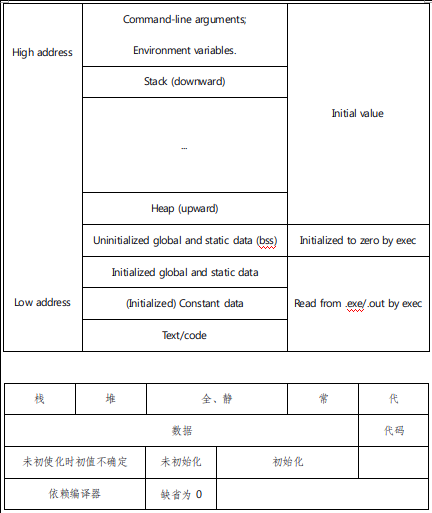
\includegraphics[width=.8\textwidth]{cMemoryLayout2}
  \caption{C Memory Layout}
  \label{fig:c-memory-layout}
\end{figure}

图~\ref{fig:c-memory-layout}~给出了虚拟内存的安排,简洁地说,就两部
分,代码区和数据区。数据区按作用域、生命周期可分堆、栈、常量、全局、
静态。对于全局和静态变量,按是否初始化,分为初始化和未初始化。常量
肯定算作初始化的。其中的 uninitialized data,也即 BSS 表示 ``block
started by symbol''. 总结来看是:\uline{堆,栈,常,代,全、静(初
  始化或未初使化)}。

特别的,图中的最高地址处的命令行参数和环境变量也算作是栈,只不过是
程序在加载时分配,相当于最早入栈的。其中命令行参数部分是传给 main 函数
的 argc 和 argv. 程序运行时还可以指定环境变量,而不是用系统默认的,
如语言编码等。如 \verb|LC=zh_CN.GB18030 ./a.out arg1|.

那么编译后的可执行文件如 a.out (Linux 的 ELF 格式) 或 .exe 是什么样的结构呢?可执行文件
里没有 BSS 段,因为还没有值,只有真正执行时才会有对应的内存。同理
栈、堆也不存在,这三部分只对进程有意义。只有常量,初始化过的全局和
静态变量。不过可执行文件还包含符号表,段表,库链接表,调试等内容。

堆需手动分配、释放,常用 new/delete 和 malloc/free 操作,由低地址往
高地址增长。堆的特点是可根据需求动态分配大小 dynamic allocation on
demand. new/malloc 在堆上分配的内存空间是全局有效的。如果不手
动 delete/free, 则这些分配到的内存在程序执行过程中一直被其占据,直
到程序结束,造成常说的“内存泄露”,导至程序被卡死。所以通常在相同作
用域内申请和释放(如函数内)。

栈是机器自动分配、释放。主要放函数参数,局部变量(自动变量)等。栈上内存主只在
函数局部才有效,函数结束会立即被释放。相反,栈的增长方向是由高往低,
这样是合理的,如果往同一个方向增长,不便于两个区间的管理。

常量区是指存放常量的地方,如:

\begin{lstlisting}
char * p = "hello, world";
printf("%d", 3);
\end{lstlisting}

里 p 是自动变量,分配在栈上。但是字符串 ``hello, world'' 和数字 3
这样的属于量放在常量区。常量区也算作初始化区的一部分。

代码区不用说就是存放放程序代码的地方。

全局变量区是指存放全局变量的地方。静态区是放静态变量的地方。通常这
两个区是合并在一起的。而且这个“全静区”是可以分成未初始化区和已初始化
区两部分。

程序执行时,先把可执行文件(代码,常量,已初始化全、静变量)加载进
内存低地址,再分配未初始化的全、静变量空间。进一步环境变量和程序参
数入栈。后面就是在运行时栈和堆的操作了。

说了这么多,我们来看看 Linux ELF 可执行方件的结构:

\begin{lstlisting}[language=bash,caption={EFL Layout},label={lst:elf-layout}]
  zack@tux ~/workspace/c $ size a.out
   text    data     bss     dec     hex filename
   2391     616      16    3023     bcf a.out
\end{lstlisting}

这里 text 指代码段大小,data 是已初使化全、静变量和常量段大小,bss
段内数据全零。后面的 dec 和 hex 是前面列的和。

\section{数组和链表}

数组和链表都是线性存储结构,但实现方法不同,通常前者在栈上由机器自
动分配,后者在堆上由程序动态分配。实现方法的不同表现出对应的优缺点。

\begin{table}[!htb]
  \centering
  \begin{tabular}{c|c|c}
    \toprule
    \diagbox{优缺点}{结构} & 数组 & 链表 \\
    \midrule
    访问 & 通过下标随机放问 & 要遍历链表顺序查找 \\
    增删 & 慢:要先扩容再移动元素 & 快:只需修改指针指向 \\
    \bottomrule
  \end{tabular}
  \caption{数组和链表}
  \label{tab:array-linkedList}
\end{table}

如果是在中间插入删除(如有序结构),则数组更麻烦,移动的元素更多。

%%% Local Variables:
%%% mode: latex
%%% TeX-master: "main"
%%% End:

\chapter{CPP}
\label{cha:cpp}


%%% Local Variables:
%%% mode: latex
%%% TeX-master: "main"
%%% End:

\chapter{Python Programming}
\label{cha:python-programming}

\section{ABCs}
\label{sec:py-abcs}

\begin{enumerate}
\item \href{https://stackoverflow.com/a/1520342}{Dynamic
    typing}. Contrary to static language, dynamic programming
  don't have declaration or data type associated.
\item Interpret and execute: source code -> bytecode -> machine
  code. It is different from C/CPP compilation.
\item Object-oriented Programming (OOP). Everything is object,
  variables included.
\item Easy but powerful language for scripting and rapid
  application development.
\end{enumerate}

\paragraph{Dynamic versus Static}

Static typed programming language do \textit{type checking}
(i.e. the process of verifying and enforcing the constraints of
types) at \textit{compile-time} as opposed to run-time. Type is
associated with compile-time identifiers.

Dynamic typed programming language do \textit{type checking} at
\textit{run-time} as opposed to compile-time. Type is associated
with run-time values.

\begin{lstlisting}[language=python,caption={Python Type Checking},label={lst:py-type-checking}]
def silly(a):
    if a > 0:
        print('greater than zero')
    else:
        print(5 + '3')


silly(1)
silly(-1)
\end{lstlisting}

Statement \verb|silly(1)| executes perfectly fine and prints
'greater than zero'. Immediately, the next statement
\verb|silly(-1)| raises type error:

\begin{lstlisting}
TypeError: unsupported operand type(s) for +: 'int' and 'str'
\end{lstlisting}

\section{Terminology}
\label{sec:py-terminology}

\begin{enumerate}
\item the prompt of shell.
\item Procedure-oriented programming (imperative); functional
  programming (declarative).
  \begin{enumerate}
  \item imperative statement vs functional exprenssion/declaration.
  \item a statement may include an expression (including
    assignment) or may be just a definition or declaration.
  \item the key diff is \textit{side effect}.
  \end{enumerate}
\item literal constants: number \& string
\end{enumerate}

\section{Execution}
\label{sec:py-execution}

To execute Python code, we have basically two forms, namely the
\textit{interactive shell} and \textit{source code
  interpretation}.

To get out of an interactive envrionment, we press \verb|Ctrl-d|
or input \verb|exit()|. Please be noted to add the parentheses pair.

\section{Syntax}
\label{sec:py-syntax}

Preliminary summaries:

\begin{itemize}
\item Comments are any text to the right of a \# symbol.
\item Literal constants include \textit{numbers} (integers and
  floats) and \textit{strings}, like \verb|52.3E-4|.
  \begin{itemize}
  \item Compared to literal constants, Python has
    \textit{variable} which store values that vary during execution.
  \item There is no separate integer type such as \textit{long} or
  \textit{short}.
  \item There is no separate \textit{char} type either.
  \item Strings are enclosed with single, double and even triple
    quotes. Triple quotes can span over multiple lines. Choose one
    appropriately. For instance, for a string containing both
    double and single quotes, we use triple quotes on the outer side.
  \end{itemize}
\item Apart from numbers and strings, we can define our own
  variable types as \textit{class}.
\item Python starts counting from $0$.
\item Surround top-level function and class definitions with two blank lines.
\end{itemize}

\section{Identifier}
\label{sec:py-identifier}

Variables are just an example of identifiers. Identifiers are
names given to identify something such as variables, function
names, class etc.

Identifiers follow the following rules:

\begin{itemize}
\item The first character must be a letter of alphabeta (ASCII) or an
  underscore \verb|_|.
\item The rest of an identifier can consist of letters,
  underscores, and digits.
\item Identifiers are case-sensitive.
\end{itemize}

Examples of invalid identifiers are:

\begin{lstlisting}
2things, this contains spaces, my-name, <abc
\end{lstlisting}

\verb|_my_name| is a valid identifier.

\section{Strings}
\label{sec:py-strings}

As mentioned in the above section, strings belong to literal
constants that are immutable like that in C/CPP. However, we can
construct a new string by different techniques such as the
\textit{format} method.

\begin{lstlisting}[language=python,caption={Python Strings},label={lst:py-strings}]
# comment to the right of symbol '#'
print('hello, world')

# number and string
age = 20
name = 'jimgray'

# 0 and 1 represents the argument indices
print('{0} is {1} years old when he went to HKUST'.format(name, age))
print('He was at his {1} years old'.format(name, age))
# give parameter a name
print('we can name the parameters: {name} is {age}'
      'years old when he went to HKUST'.format(name=name, age=age))
print('{0:.3f}'.format(1.0/3))
print('{0:_^11}'.format('hello'))
# formated string (f-string) is an expression evaluated at runtime
print(f'his name is {name} and he is {age} years old.')
print('''this a multi-line string.
The second sentence.''')
\end{lstlisting}

\textit{print} append newline \verb|\n| to each statement. We can
specify the \textit{end} parameter to terminate this behaviour
like:

\begin{lstlisting}[language=python]
print('a', end='')
print('b', end='')
\end{lstlisting}

\subsection{Escape Sequence}
\label{sec:py-escape-sequence}

Although we can enclose a string containing a quotatation mark
with double quotes, \textit{backslash} can escape special
symbols. For example, \verb|"what's your name"| are equal to
\verb|'what\'s your name'|.

To escape the backslash itself, we use double backslash like
\verb|\\|.

If we want to specify a two line string, just insert a \verb|\n|
symbol. Similarly, we have \verb|\t| for tabular symbol.

You may already know that a bare backslash at the end of line
continues the previous element like:

\begin{lstlisting}
"this is the 1st string. \
this is the 2nd string."
\end{lstlisting}

\subsection{Raw String}
\label{sec:py-raw-string}

Raw string means ignoring escape sequences within the string. Just
prepend the string with \verb|r| or \verb|R|.

\begin{lstlisting}[language=python,caption={Raw String},label={lst:raw-string}]
r"Newlines are indicated by \n"
\end{lstlisting}

When dealing with \textit{regular expression}, we'd better use raw
string, which otherwise would require a log of backslash escaping.

%%% Local Variables:
%%% mode: latex
%%% TeX-master: "main"
%%% End:


\part{Networking}
\chapter{TCP/IP}
\label{cha:tcpip}

\section{Segment Datagram and Frame}
\label{sec:segment-datagram-frame}

Before everything else, let's have a look at terminologies
\textit{segment}, \textit{datagram} and \textit{frame}.

Generally speaking, they refer to a \textit{unit} of data
transmitted through the protocol stack without differentiating
protocols.

However, when talking about \textit{segment}, we mean a TCP
packet, including both the TCP headers and TCP payload. On the
other hand, \textit{datagram} means payload and headers of an IP
packet. The two terms are also called \textit{packet} in
general. Interestingly, a UDP packet is also called
datagram. Maybe this is due to UDP's \textit{at best} strategy.

Lastly, a \textit{frame} is a \textit{Link layer} (mostly the
Ethernet) unit. But it is weird to call it a packet.

You may also hear of \textit{fragment}. When an IP datagram is too
large to fit a MTU \ref{sec:mss-mtu}, the payload part is split
into smaller parts, forming multiple new units. This is also
called \textit{fragmentation}.

By the way, in the Physical layer, we usually use
\textit{transmit} or \textit{transmission}. More details about
those terms, read
\href{https://stackoverflow.com/a/11637061}{Definition of Network
  Units}.

\section{MTU and MSS}
\label{sec:mtu-mss}

Let's talk about \textit{Maximum Transmission Unit (MTU)}
first. It is the largest IP packet that can be transmitted over
\textbf{all} links from source to destination. So MTU refers to
the maximum payload of Ethernet frames, \textbf{not} including
frame headers (20 bytes).

It is a physical parameter (i.e. set in router) that specifies the
size of the largest protocol data unit (i.e. IP datagram) that can
be sent in a single link layer transmission. MTU usually appear in
association with network Interfaces (i.e. routers, PC NICs, serial
ports etc.).

\textit{Maximum Segment Size (MSS} is confined to MTU. It refers
to the maximum amount of application-layer data that can be placed
in a TCP segment, \textbf{not} including segment headers or Option
fields. So we can say it is a parameter of the \textit{Options
  fields}. Although it is named after \textit{segment}, MSS does
not count TCP headers and Options field.

So both terms refer to payload only! Their relations can be
expressed by equation \eqref{eq:mtu-mss}.

\begin{equation}
  \label{eq:mtu-mss}
    \text{MTU} = \text{IP Headers (20 bytes)} + \text{TCP Headers (20 bytes)} \text{ [+ TCP Options]} + \text{MSS}
\end{equation}

For general Ethernet links, MSS is $1500 - 20 - 20 = 1460$. For
Point-to-Point Protocol over Ethernet (PPPoE), it requires extra 8
bytes (6 bytes PPPoE plus 2 bytes PPP) overhead. Therefore the MTU
is $1500 - 8 = 1492$ bytes and corresponding MSS is 1452 bytes.

% https://blog.zenlab.it/traceroute-vs-ping-vs-mtr/

%%% Local Variables:
%%% mode: latex
%%% TeX-master: "main"
%%% End:

\chapter{Data Bills}
\label{cha:data-bills}

\section{Contact}
\label{sec:billing-contact}

\begin{table}[!h]
  \centering
  \begin{tabular}[!h]{c}
    \toprule{}
    HU Zhan \\
    zhan.hu@chinacache.com \\
    \bottomrule
  \end{tabular}
  \caption{Contact}
\end{table}

\section{95th Percentile}
\label{sec:95th-percentile}

\textit{95th percentile} is a commonly used commercial scheme to
calculate and evaluate the regular and sustained used of a network
connection. It is a kind of
\href{https://en.wikipedia.org/wiki/Burstable_billing}{Burstable
  Billing} that measures bandwidth based on \textit{peak use}.

Generally, it allows the usage to exceed a specified threshold for
a short period of time without the financial penalty of purchasing
a higher
\href{https://en.wikipedia.org/wiki/Committed_information_rate}{Committed
  Information Rate} (CIR is another billing method) from an ISP.

There are two critical factors involved in this scheme, namely the
\textit{percentile} and the \textit{sampling interval}. Usually,
they are 95\% and 5m respectively and therefore it is also called
\textit{95/5 percentile} (or \textit{95 percentile}).

Given a monthly billing cycle, 95/5 percentile allows a customer
to have a short (i.e. threshold is $30 \times 24 \times 5\% = 36$
hours) burst in in traffic without overage charges. More
specifically, bandwidth could be used at a higher rate for up to
$24 \times 60 \times 5\% = 72m$ a day with no financial
penalty. That is to say, 95\% of the time, the usage is below this
amount. Conversely, 5\% of the samplings may be bursting above
this rate.

\begin{figure}[!htb]
  \centering
  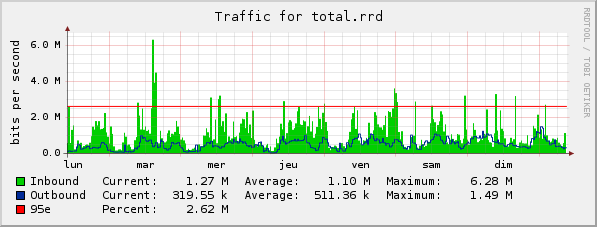
\includegraphics[scale=.6]{burstableBilling}
  \caption{95/5 Percentile}
  \label{fig:95-percentile}
\end{figure}

How is \textit{this amount} or \textit{this rate} is calculated?
Usually a time-bandwidth chart is drawn to visualize bandwidth
usage through a bill cyle like figure \ref{fig:95-percentile}
whose \textit{integral area} reflects the total data transmitted.

Bandwidth is sampled at an interval of 5 minutes from the switch
or router. During an interval, the average bandwidth is calculated
as the number of bits transferred throughout the interval divided
by the duration (5m = 300s).

At the end of the month, all the bandwidth samples
($30 \times 24 \times 60 \div 5 = 8640$) are sorted from highest
to lowest. The top 5\% ($8640 \times 5\% = 432$) samples is thrown
away and the next highest sample $432 + 1 = 433$ becomes the
billable use for the entire month. Obviously,
$432 \times 5 \div 60 = 36h$.

In the figure \ref{fig:sorted-95th-percentile}, the
billable value falls around 6Mbps, or 60\% of the highest
burst. From this figure, we find the sorted slope is quite
steep. The sharp burst contributes a lot to the final bill though
not much bandwidth is used (small area).

\begin{figure}[!htb]
  \centering
  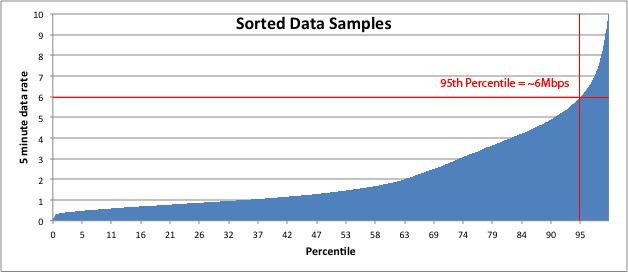
\includegraphics[scale=.5]{95th-chart-sorted}
  \caption{Sorted Percentile}
  \label{fig:sorted-95th-percentile}
\end{figure}

Conversely, at any moment during the billing cycle, even if peak
traffic only appears for a short \textit{instant} and no
additional traffic is generated, the billing amount can be
sbustantially higher than average usage billing. This is not the
end of the story. Although we get the billable value, it may not
take affect when paying bills. For example, what if all customers'
95th percentile value are pretty small? In that case, the ISP's
infrastructure would be wasted and lose money.

In reality, 95th percentile assumes a \textit{base commit rate}
(and fees associated) that must be guranteed by customers. The
95th percentile value only takes effect when it is higher than the
base commit rate, otherwise the base value would be used
irrespective of the 95th percentile. The higher the base commit
rate is, the cheaper the bandwidth fee becomes.

Base commit rate is \textit{not} CIR (where hard bandwidth must be
reserved for a customer) but just a billing gurantee even the real
bandwidth usage is 0. It is fairly to both the carrier and the
customer in terms of the service delivered to the customer and the
ability of the carrier to scale its infrastructure to meed
different customers' needs.

\section{Other Billing Methods}
\label{sec:other-billing-methods}

The 95th percentile is utilized mostly between ISP and business
customers in a datacenter while CIR is adopted between ISP and
individuals for home cable, fiber, DSL etc. Hard bandwidth is
guranteed and no burst is allowed. Customers pay for the fixed
bandwidth value.

Apart from 95th percentile and CIR, \textit{actual throughput
  billing} is used in limited and shared bandwidth networks like
mobile data networks (i.e. 4G) where where resources
overprovisioning is not possible due to limited spectrum
availability. Customers just pay for what they get on demand. ISP
will simply record how much data you moved over the circuit for
that interval. It is also used by some web-based VPS platforms to
bill customers.

You can read more about billing methods on
\href{https://www.semaphore.com/95th-percentile-bandwidth-metering-explained-and-analyzed/}{billing
  methods explained and analyzed} and check figure
\ref{fig:billing-methods}.

\begin{figure}[t]
  \centering
  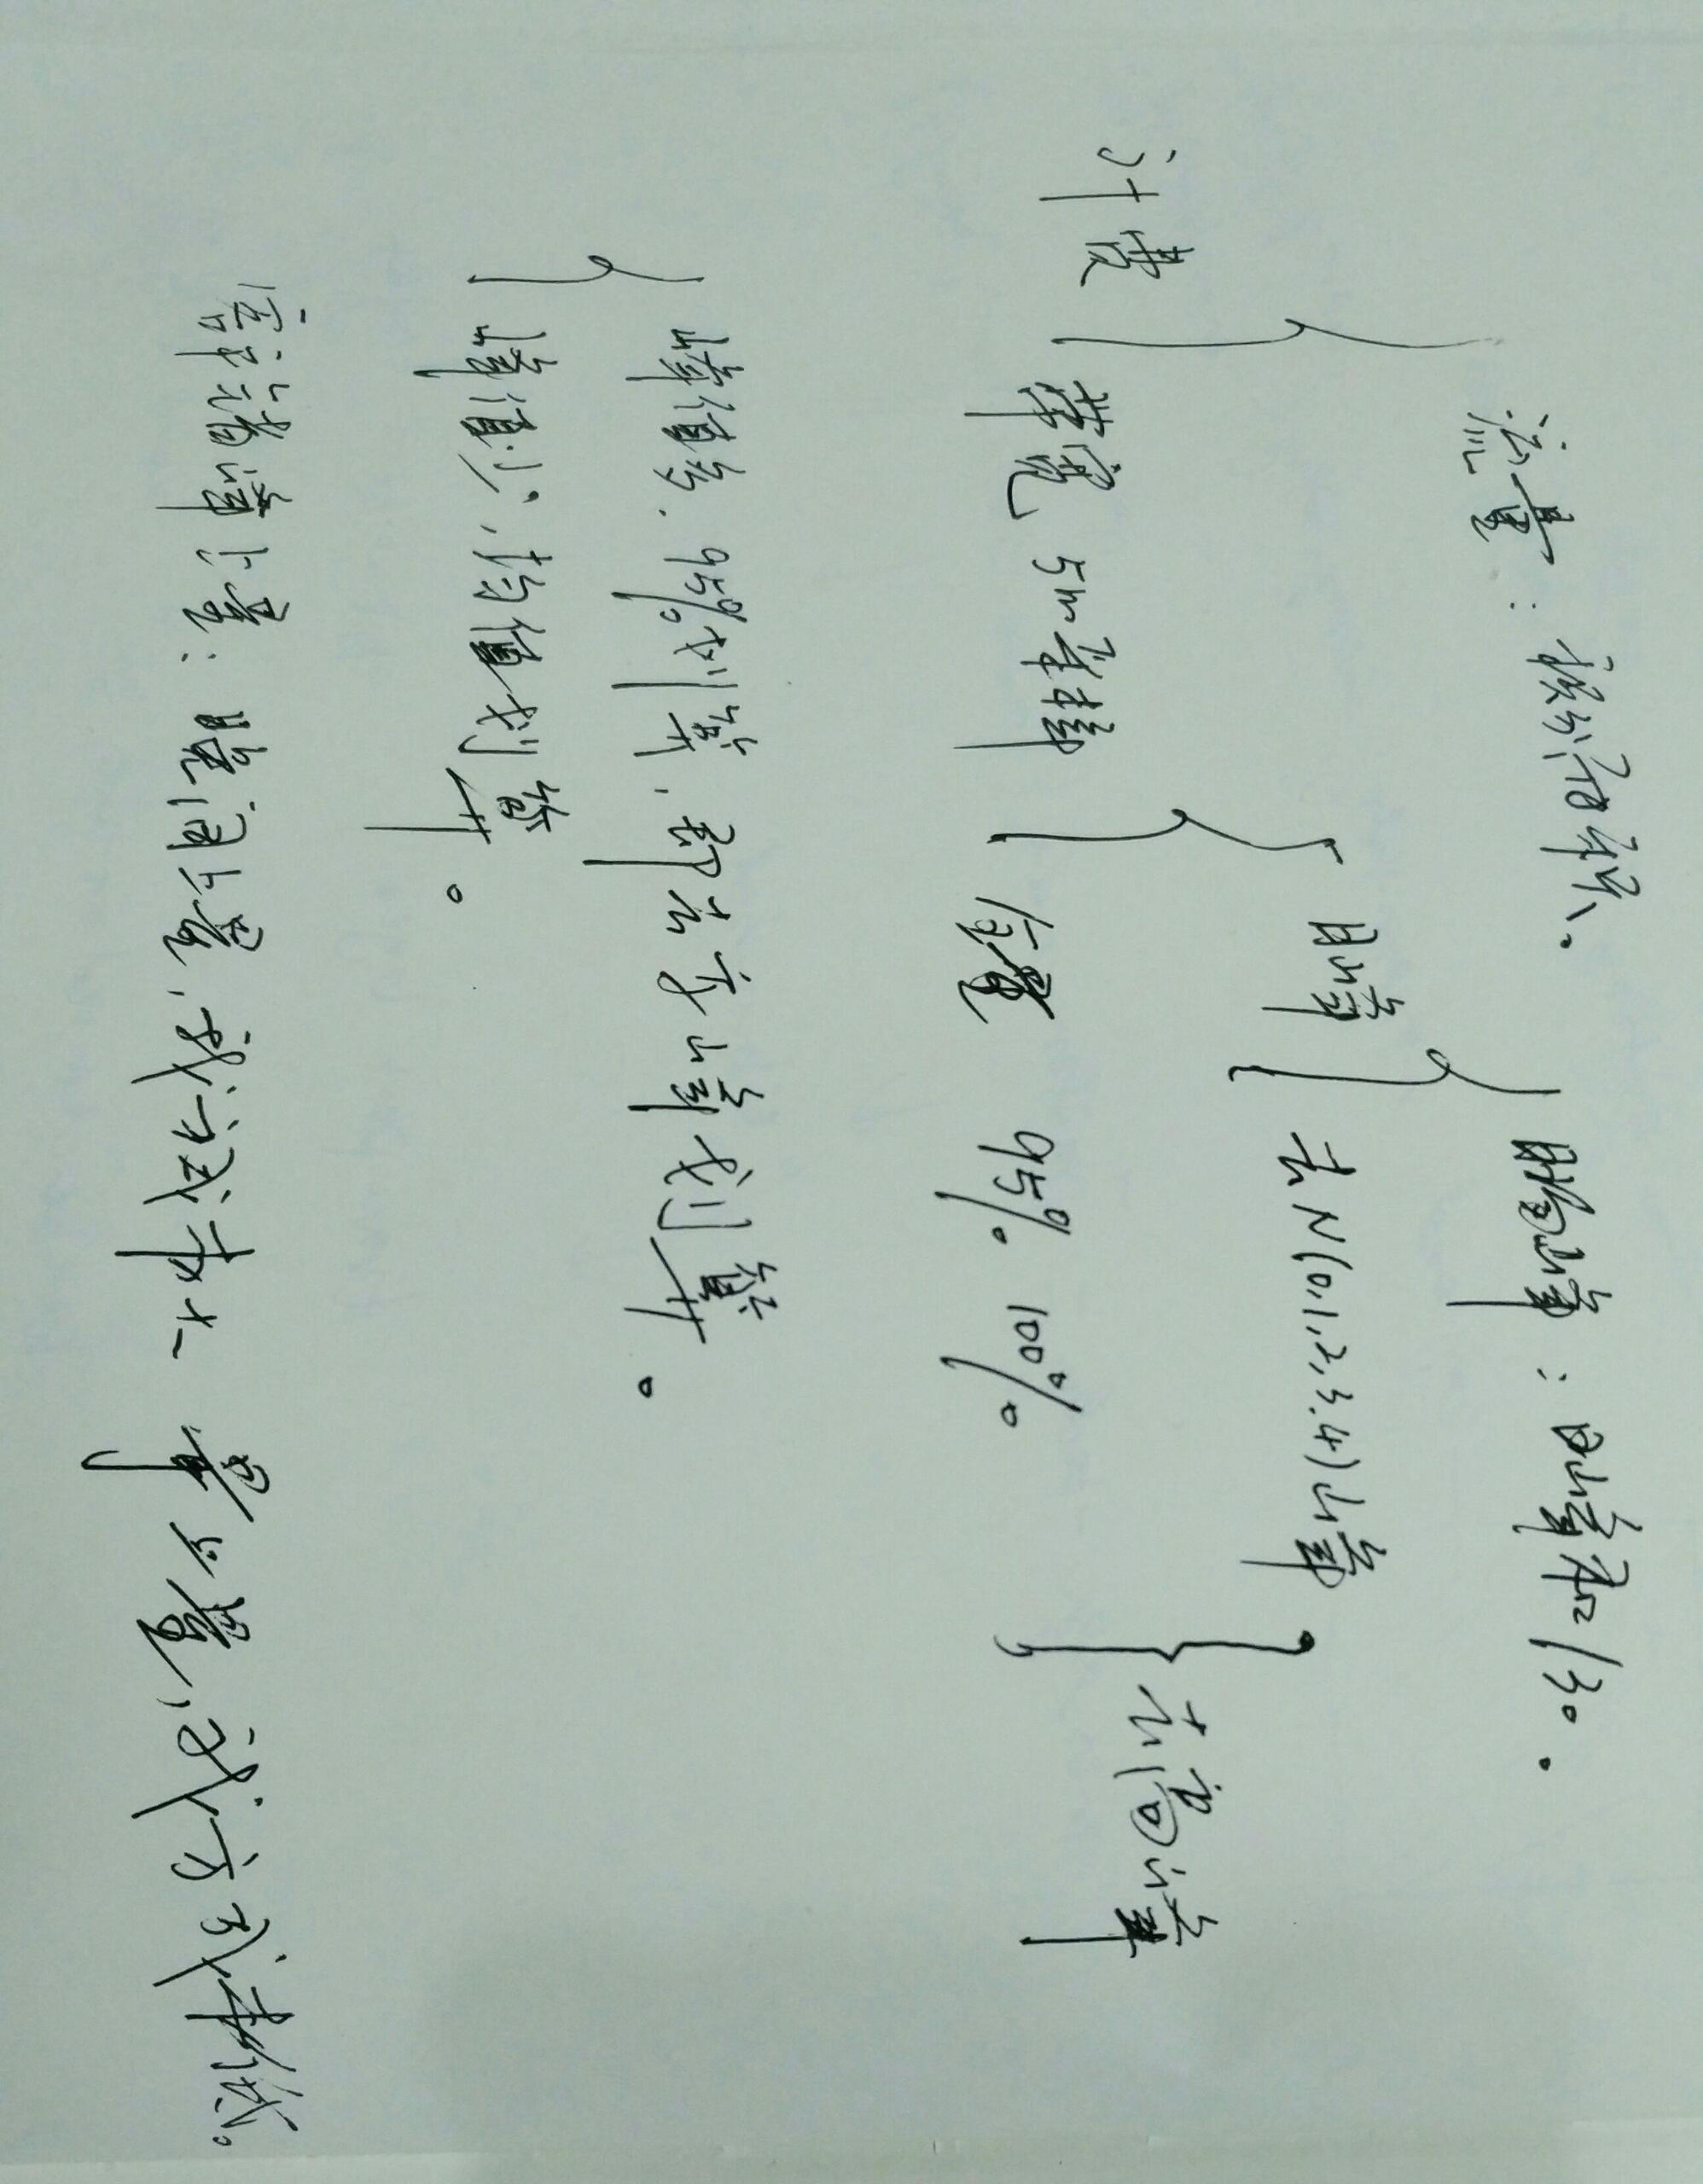
\includegraphics[scale=0.17,angle=90]{data-billing}
  \caption{Billing Methods}
  \label{fig:billing-methods}
\end{figure}

%%% Local Variables:
%%% mode: latex
%%% TeX-master: "main"
%%% End:

\chapter{Networking Tools}
\label{cha:networking-tools}

% https://blog.zenlab.it/traceroute-vs-ping-vs-mtr/


%%% Local Variables:
%%% mode: latex
%%% TeX-master: "main"
%%% End:


\part{Brainteaser}
\chapter{Brain Teasers}
\label{cha:brain-teasers}

\subsubsection{补全数列空缺}

例 3 5 10 25 75 () 875. 观察此数列发现,相邻两项的数间没有什么特别关系,
相乘相加都不是。这时应考虑相邻三、四项项的关系,会发现 $3 \times 5 + 10
= 25$, 类似地有 $5 \times 10 + 25 = 75$. 因此空处的值应是 $10
\times 25 + 75 = 325$. 再来一个例子,5 6 16 28 60 (). 分析得出
$5 \ times 2 + 6 = 16$, 还有 $6 \times 2 + 16 = 28$. 所以空处的值
应是 $28 \times 2 + 60 = 116$. 此两例考虑连续多个数之间的递推关系,
类似于 Fibonacci Sequence.

\subsubsection{牛吃草}

一块匀均生长的草地,可供 27 头牛吃 6 周,或 23 牛吃 9 周,问多少牛
可吃 18 周?

我们先设一头牛吃草的速度是 a, 单位可以是 kg/w, 则 6 周吃 $27 \times 6
\cdot a$ kg 的草。设草的生长速度是 b, 单位可以是 kg/w, 那么 6 周
长了 $6 \cdot b$ kg 的草。那么是不是 $27 \times 6 \cdot a = 6b$ 呢?

不是!因为牛吃草前,草地上本来就有部分草,设为 c kg, 则 $27 \times
6 \cdot a = 6b + c$, 同理我们得出:

\[
  \begin{aligned}
    27 \times 6 \cdot a &= 6 \cdot b + c \\
    23 \times 9 \cdot a &= 9 \cdot b + c \\
    x \times 18 \cdot a &= 18 \cdot b + c \\
  \end{aligned}
\]

通过前两个方程,可得出 $b = 15 \cdot a$ 和 $c = 72 \cdot a$, 进而求出 $x = 19$.

\subsubsection{相向而行}

甲乙两地相距 90 米,A, B 二人分别从甲乙同时出发,在两地来回跑动。甲
的速度是 3 m/s,乙的是 2 m/s. 问 10 分钟内甲乙相遇几次?

第一次相遇时二人行使 90 米,时间是 $90 \div (3 + 2) = 18$s. 相遇后
二人背向而行,直至达到对端。此时二人又行使了 90 米,用时 18s.

二人再次相向而行,准备下一次相遇。此后一直重复此过程。可以发现相遇
一次二人行使了 180 米,花时 36s, 所以 10 分钟相遇次数是 $10 \times
60 \div 36 = 16\frac{2}{3}$, 结果是分数,那么是 16 次还是 17 次呢?

应是 17 次,因为第次相遇时,在 36s 的前半程,所以分数部分应四舍五
入!

上面这种方法不够明了。第一次相遇需 18s, 下一次相遇需 36s, 再下一次
相遇需 36s, 此后每一次相遇都需 36s. 我们找相遇的时间点更合理,得到
一个等差数列:

\[
  \begin{aligned}
    t_1 &= 18 \\
    t_2 &= 18 + 36 \\
    ... \\
    t_n &= 18 + (n - 1) \cdot 36
  \end{aligned}
\]

根据 $t_n = 10 \times 60$ 可以算出 $n = 17\frac{1}{6}$. 由此可知,
相遇 17 次,因为剩下的 1/6 还没到第 17 次相遇时间点。

\subsubsection{背向而行}

有一 300 米圆跑道,甲乙在同一地点背向而行,速度分别是 3.5m/s 和
4m/s. 问第 10 次相遇时,甲离出发地还有多远?

每相遇一次,两人共行走了 300 米,其中甲行走了 $\frac{3.5}{(3.5 +
  4)} \times 300 = 140$ 米,而乙行走了 160 米。

那么相遇 10 次时,甲累计走了 $10 \times 140 1400$ 米,而 $1400
\div 300 = 4\, \cdots \cdots\, 200$, 也就是说走了 4 圈后,第 5 圈走了
200 米,所以离出发点还剩 100 米。

\subsubsection{交换变量}

有两个整数 a = 5, b = 7, 不通过临时变量,如何交换二者的值?

方法一:异或 XOR. 异或的意思是,让两个数的二进制位互相比对,同为 0
或 1 时结果为 0, 有一个 1 一个 0 (相异)时结果为 1. 所以任何数异
或自己的结果是 0. 对应的 C 语言结果是:

\begin{lstlisting}[ language=C,caption={Swap by XOR} ]
a = a^b;
b = a^b;
a = a^b;
\end{lstlisting}

方法二:加减法。

\begin{lstlisting}[ language=C,caption={Swap by Arithmetic Operations} ]
a = a + b;
b = a - b;
a = a - b;
// Or
a = (a + b) - (b = a)
\end{lstlisting}

%%% Local Variables:
%%% mode: latex
%%% TeX-master: "main"
%%% End:

\chapter{行测图行推理}

%https://www.zhihu.com/question/59668737

\section{规律总结}

首先分析图形\uline{外观},考察图形\uline{画法},得出图形里
的\uline{分部要素},也可称为\uline{元素}。

\begin{enumerate}
\item 边。三角形、四边形、五边形……
\item 曲线。
\item 圆。
\item 区。图形被分割成不同的封闭区域。
\item 交点。边上的交点。
\end{enumerate}

找出各图形元素后,再分析其\uline{规律}。

\begin{enumerate}
\item 行列。从行和列两个维度来分析规律。
\item 数量。每种元素的数量可能呈某种关系,如相等,差数列。还可
  以是行、列上数量关系。如边数,交点数,区域数等。
\item 笔画。是否是一笔画完。
\item 对称。如轴对称(竖轴、横轴),旋转对称(中心对称,180 度),
  不对称。如英文字母的对称性。还可能数对称轴(相同的、不同的)的数
  量。
\item 旋转。图形整体依次顺时针、逆时针旋转一个角度。
\item 翻转。图形整体以某轴翻转 180 度。如水平翻转。
\item 平移。某元素在图内平移一定距离。如小方格每次移顺时针移 3 个位
  置。
\item 相对。不同元素在图内相对位置发生变化。相对位置可以是内部、外
  部,相交、相接、分离,也可以是直角处、圆弧处,还可以是在最长边、
  最短边处。
\item 加减。相邻图形或元素之间加减组合出新图。如第 1 个图形和第 2
  个图形组合起来是第 3 个图形。常见的是九宫格里,行、列间图形是加
  减关系。有时甚至是先旋转再加减。
\item 类别。图形可以按其属性分类。如同为生活类用品,同属用腿、用手、
  手脚并用的运动项目。
\end{enumerate}

%%% Local Variables:
%%% mode: latex
%%% TeX-master: "main"
%%% End:


\part{Chemistry}
\label{part:chemistry}
\chapter{走进化学世界}

化学就是研究\uline{物质}及其\uline{变化},它不仅研究已经存在的物质,还
要研究和创造自然界原本不存在的新物质。例如,半导体材料,电阻几乎为零的
超导体,有记忆能力的新材料,等等。

化学在保证人类生存和提高生活质量上有很大帮助。例如:

\begin{itemize}
\item 化肥和农药,增加粮食产量。
\item 化学合成药物,指抑制细菌和病毒。
\item 化学新能源、新材料。
\end{itemize}

近代化学突破源于两点:

\begin{enumerate}
\item 物质是由分子原子构成的,分子中原子的重新组合是化学变化的基础。
\item 元素周期表。
\end{enumerate}

这两个突破使得化学研究有迹可寻。化学的科学定义:\textbf{化学是在分子、
  原子层上研究物质\uline{性质、组成、结构}与\uline{变化}规律的科学}。研
究物质是指研究其性质、组成和结构等\uline{静态特征},而变化是化学反应,
也即原子的重新组合,这是一个\uline{动态过程}。

\section{性质及变化}

物质变化分两两种:

\begin{itemize}
\item 物理变化:没有生成新物质的变化,如物质形态发生变化。气态、液态、
  固态三态之间的相互转换的过程就是物理变化。
\item 化学变化或叫化学反应:生成新物质的变化(原子重新组合),常表现为
  颜色变化,放出气体,生成沉淀等。化学变化还伴随物质能量变化,如吸热、
  放热、发光等。
\end{itemize}

虽然物理变化也通常伴随能量转换,但主要借用外部能量。而化学变化和能量可
以只来自物质本身,不需要外部能量辅助。

依据物质变化过程中表现出的性质,可有:

\begin{itemize}
\item 化学性质:物质在化学变化中表现出的性质。例如,铜在潮湿的空气中生
  成铜绿。
\item 物理性质:物质不需要化学反应就表现出来的性质。物质颜色、状态、气
  味、硬度、熔点、沸点、密度等都是物理性质。例如,常态下,氧气是种无色、
  无味的气体。注意,物理性质可能是物理变化过程表现出的性质,如物质的三
  态。
\end{itemize}

外界条件改变时,物质性质也会随着变化,因此,描述物质性质时往往\uline{要
  注明条件}。如,当温度升高时,固态冰变成液态水,再加温,水会沸腾。液体
的沸点是物理性质,但受大气圧强的影响。大气稀薄的地方,大气圧强变小,这
时水的沸点会降低,容易烧开。

\subsection{大气圧}

由于大气圧强是变化的,人们把 $1 atm = 101 kPa = 76 cm \text{水银柱重
  量}$当作标准大气圧强。大气压强是指大气对浸在它里面的物体产生的压强,
也叫大气圧或气圧,可以用空气的重力或分子热运动来解释其产生机理,而且这
两种解释是等价的。

那么如何用重力和分子热运动解释呢?在密封空间内,气圧的产生应从微观上来
解释。气体分子热运动时,撞击空间内壁,产生作用力(内壁也同时产生反作用
力),这个作用力就是气体圧力。没有内壁就不会产生气体圧力!圧强是单位面
积上的圧力,表示强度,不用考虑内壁的存在。

由于分子作用力各向同性,所以任一点的圧强在不同方向上相同。

对于空气呢?空气分子同样作热运动,但是没有内壁,怎么产生圧力呢?有地球
引力!地球引力相当于上述密闭空间内壁的反作用力。所以空气中任意一点也有
空气圧力,进而也有圧强。同理,空气圧力也是各向同性的。

至于圧强的数值计算,两种情况有所不同,关键是算出分子热运动的作用力。对
于密闭空间,它是 $P = nTR/volume$. 对于空气,因为重力和空气分子热运动产生
的撞击力平衡,大气压强是大气施加于单位面积上的重力,即该地单位面积垂直
向上延伸到大气层顶的空气柱的总重力。简单的数学公式是 $P = m \cdot
g/area$. 实际中要考虑不同高度处重力加速度 $g$ 的不同。

\section{化学实验}

\subsection{注意事项}

\begin{itemize}
\item 手不接触药品,不尝药品,鼻孔不可太靠近瓶口(特别是气体)。
\item 实验剩余药品不能放回原瓶,不能随意丢弃,不能带出实验室。要放入指
  定容器。
\item 节约药品。未说明剂量时,液体一般取 $1 - 2 \, mL$, 固体只需盖满试
  管底部即可。
\item 保护眼睛,如果进了药液,应立即用清水清洗,要眨眼睛。
\end{itemize}

\subsection{药品取用}

\begin{itemize}
\item 固体:广口瓶。药匙(粉状、颗粒)、摄子(块状),取完应擦净。玻璃
  容器横放,块状放容器口,缓缓坚立,滑入底。药匙送粉状入试管底,再直立。
\item 液体:细口瓶。倾倒法。瓶塞倒立桌面,瓶口紧挨试管口,瓶身标签面朝
  手心。定量取液,用量筒。量液时,视线与凹液面最低处保持水平。仰视偏多,
  俯视偏少。取少量液体用滴管,应保持橡胶帽朝上,不可平放、倒放,否则腐
  蚀橡胶帽或污染试剂。滴管应悬空滴液,不可接触容器口,否则因为试剂太
  少,沾在内壁。用完即洗。
\end{itemize}

\subsection{物质加热}

一般用酒精灯。不可以向燃着的酒精灯添加酒精,也不可以用一个点燃另一个。
用灯帽熄灭,不可用嘴吹。熄灭后,取下灯帽再盖上。

加热试管液体:

\begin{enumerate}
\item 试管外壁应干燥,液体不超过容积的 1/3.
\item 试管夹由试管底部套上、取下。
\item 先使试管底部均匀受热,再用外焰固定加热。
\item 试管口不要对着自己或他人。
\item 加热后的试管不能立即接触冷水或用冷水冲洗。
\end{enumerate}

\subsubsection{三层火焰}

本节顺便说下蜡烛然烧问题。蜡烛然烧时,蜡固体先熔化、气化,再与空气中氧
气发生化学反应。

外焰是红白色,温度高;而内焰为红色且边缘是蓝色,温度低。焰心没有发生燃
烧,所以不烧手。温度的高低主要由与氧气接触面积决定。外焰处氧气最多,燃
烧最充分,温度最高。焰心处氧气已消耗殆尽,所以没有燃烧。

\uline{色温}和\uline{温度}是两个不同的概念。色温反应的是单个分子的能量,
能量越高,颜色越偏蓝。温度是分子热运动的宏观测量,不仅要考虑单个分子能
量,还应考虑分子总个数。在相同分子个数情况下,蓝焰温度肯定比黄色或红色
高。

但在蜡烛然烧时,外焰温高除了氧气多外,和热气体上升也有关系。另外,既然
外焰燃烧更充分,为何不见蓝色。实际是有蓝色的,只是被遮住了。外焰处蜡蒸气
非常多,被外焰加热后,变成白炽色,把燃烧的蓝色吸收了。所以外焰的高温不
是因为黄色,而是蓝色(充分燃烧)和上升热气。

\subsection{仪器连接}

玻璃管,胶皮管,橡胶塞:

\begin{enumerate}
\item 玻璃管和橡胶塞:玻璃管口用水湿润,对准橡胶塞上的孔稍用力转动、插入。
\item 玻璃管和胶皮管:玻璃管口用水湿润,稍用力即可插入。
\item 容器口和橡胶塞:慢慢转动橡胶塞,塞入容器口(如试管)。
\item 气密性检查:用手握紧试管,观察水中导管口是否有汽泡冒出,有则好。
\end{enumerate}

\subsection{洗涤玻璃容器}

必需洗涤玻璃容器,否则影响实验效果。以洗试管为例:

\begin{enumerate}
\item 倒掉废液。
\item 注入半试管水,振荡后再倒掉。
\item 重复上一步聚。
\item 如试管内壁还有不易洗掉残留物质,用试管刷刷洗。洗刷时,须转动或上
  下移动试管刷。
\end{enumerate}

洗过的玻璃容器内壁附着的水既\uline{不聚成水滴,也不股下流},表明仪器已
洗干净。

\chapter{空气}

\section{简介}

空气的主要成分是氮 78\%, 氧 21\%, 稀有气体 0.94\%, 二氧化碳 0.03\%, 其
它气体和杂质占 0.03\%. 其中氮和氧几乎各占 1/5 和 4/5. 稀有气体主要是氦
hài, 氖、氩、氪、氙 xiān, 氡等。
                     
\begin{itemize}
\item 混合物:由两种或两种以上的物质混合而成的物质。组成混合物的各种成
  分保持着它们各自的性质。
\item 纯净物:只有一种物质组成。纯净物可以用\uline{化学式}表示,如氮气
  是 \ce{N2}, 磷是 \ce{P}, 五氧化二氮是 \ce{P2O5} 等。
\end{itemize}

\section{成分}

各主要成分。












\chapter{物质列表}

\begin{table}[!htb]
  \centering
  \begin{tabular}[!htb]{r|c|c}
    \toprule
    \diagbox{化学式}{叁数} & \text{名称、别名} & \text{颜色和状态} \\
    \midrule
    \ce{CuSO4} & 硫酸铜、胆矾、蓝矾 & (无水)灰白色粉未、(有水)
    蓝色结晶固体 \\
    \ce{H2O} & 水 & 无色液体 \\
    \ce{KAl(SO4) * 2H2O} & 十二水合硫酸铝钾、明矾 & 无色或白色的八面体晶体 \\
    \ce{Fe} & 铁 & 银白色固体 \\
    \ce{Al} & 铝 & 银白色固体 \\
    \ce{O2} & 氧气 & 无色无味气体 \\
    \bottomrule
  \end{tabular}
  \caption{常见物质列表}
  \label{tab:common-substances}
\end{table}


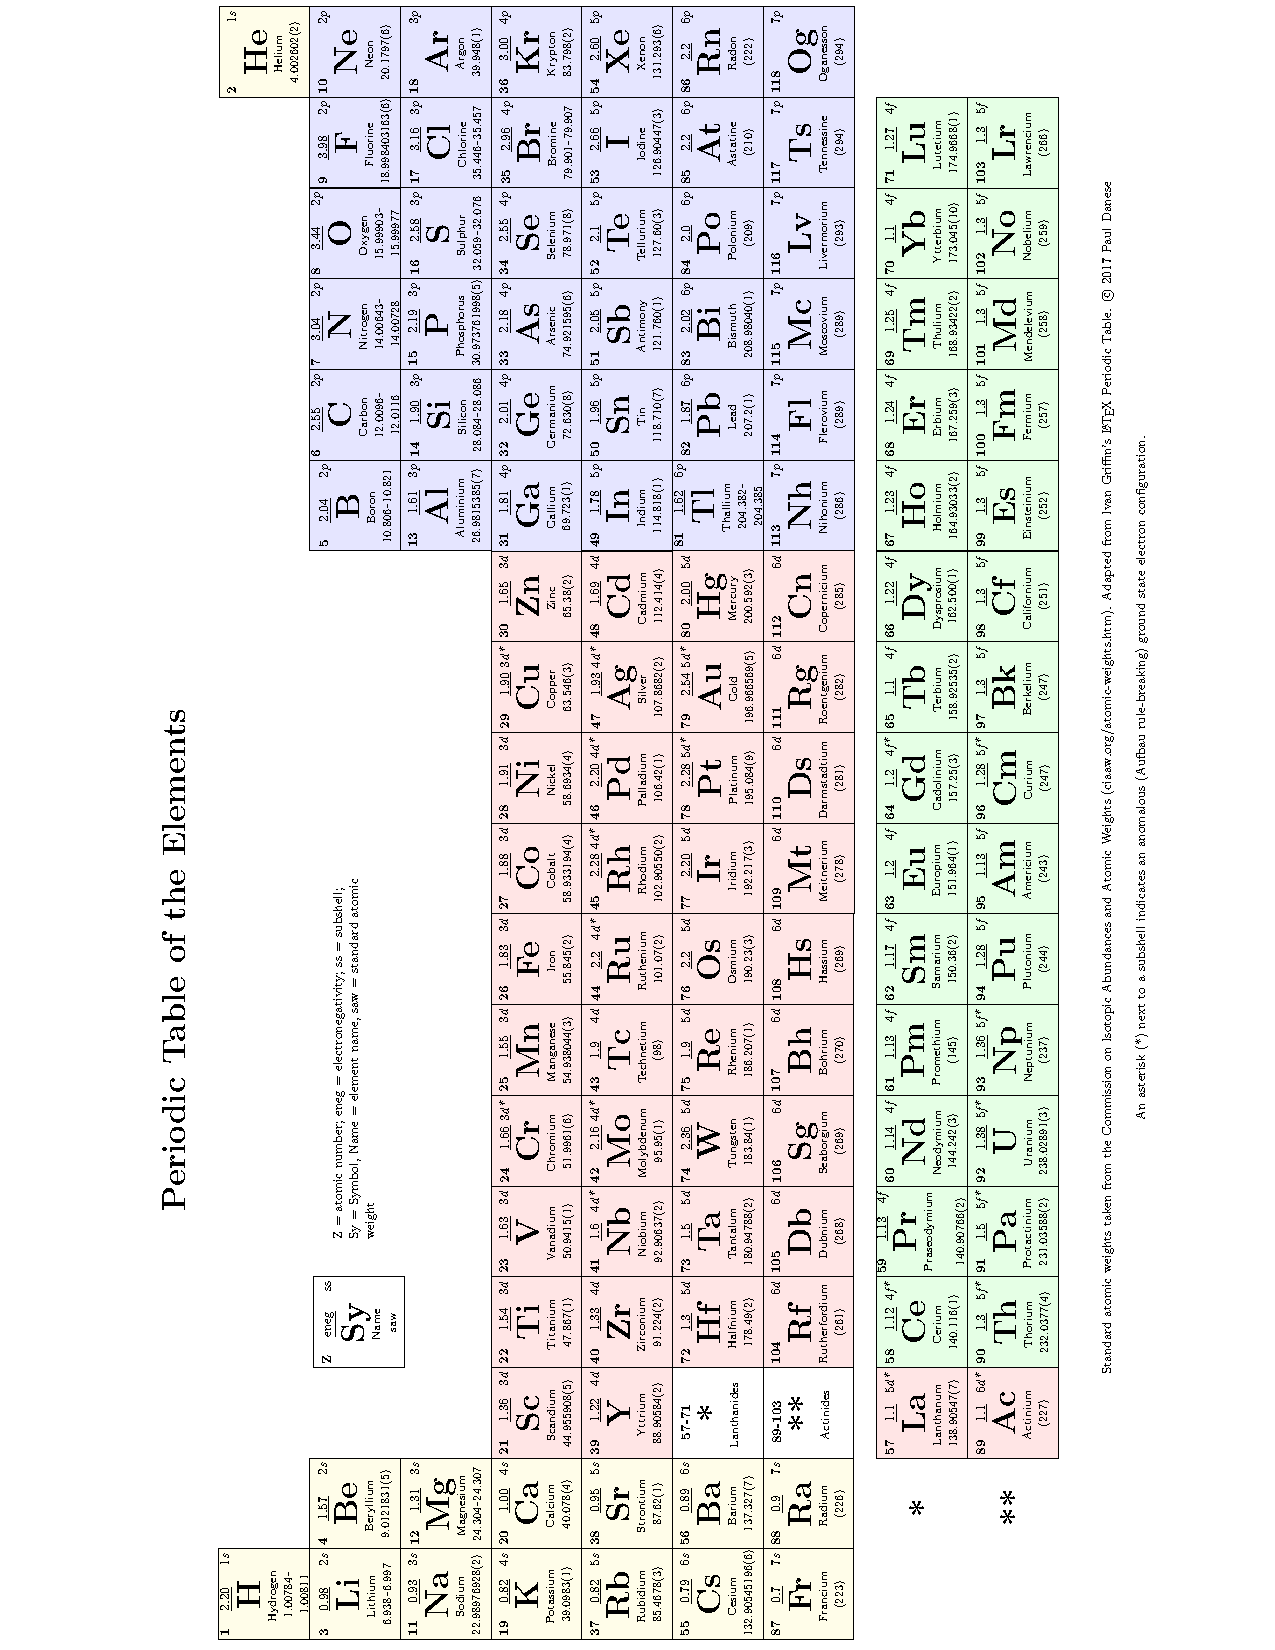
\includepdf[pages=-]{periodic_table.pdf}
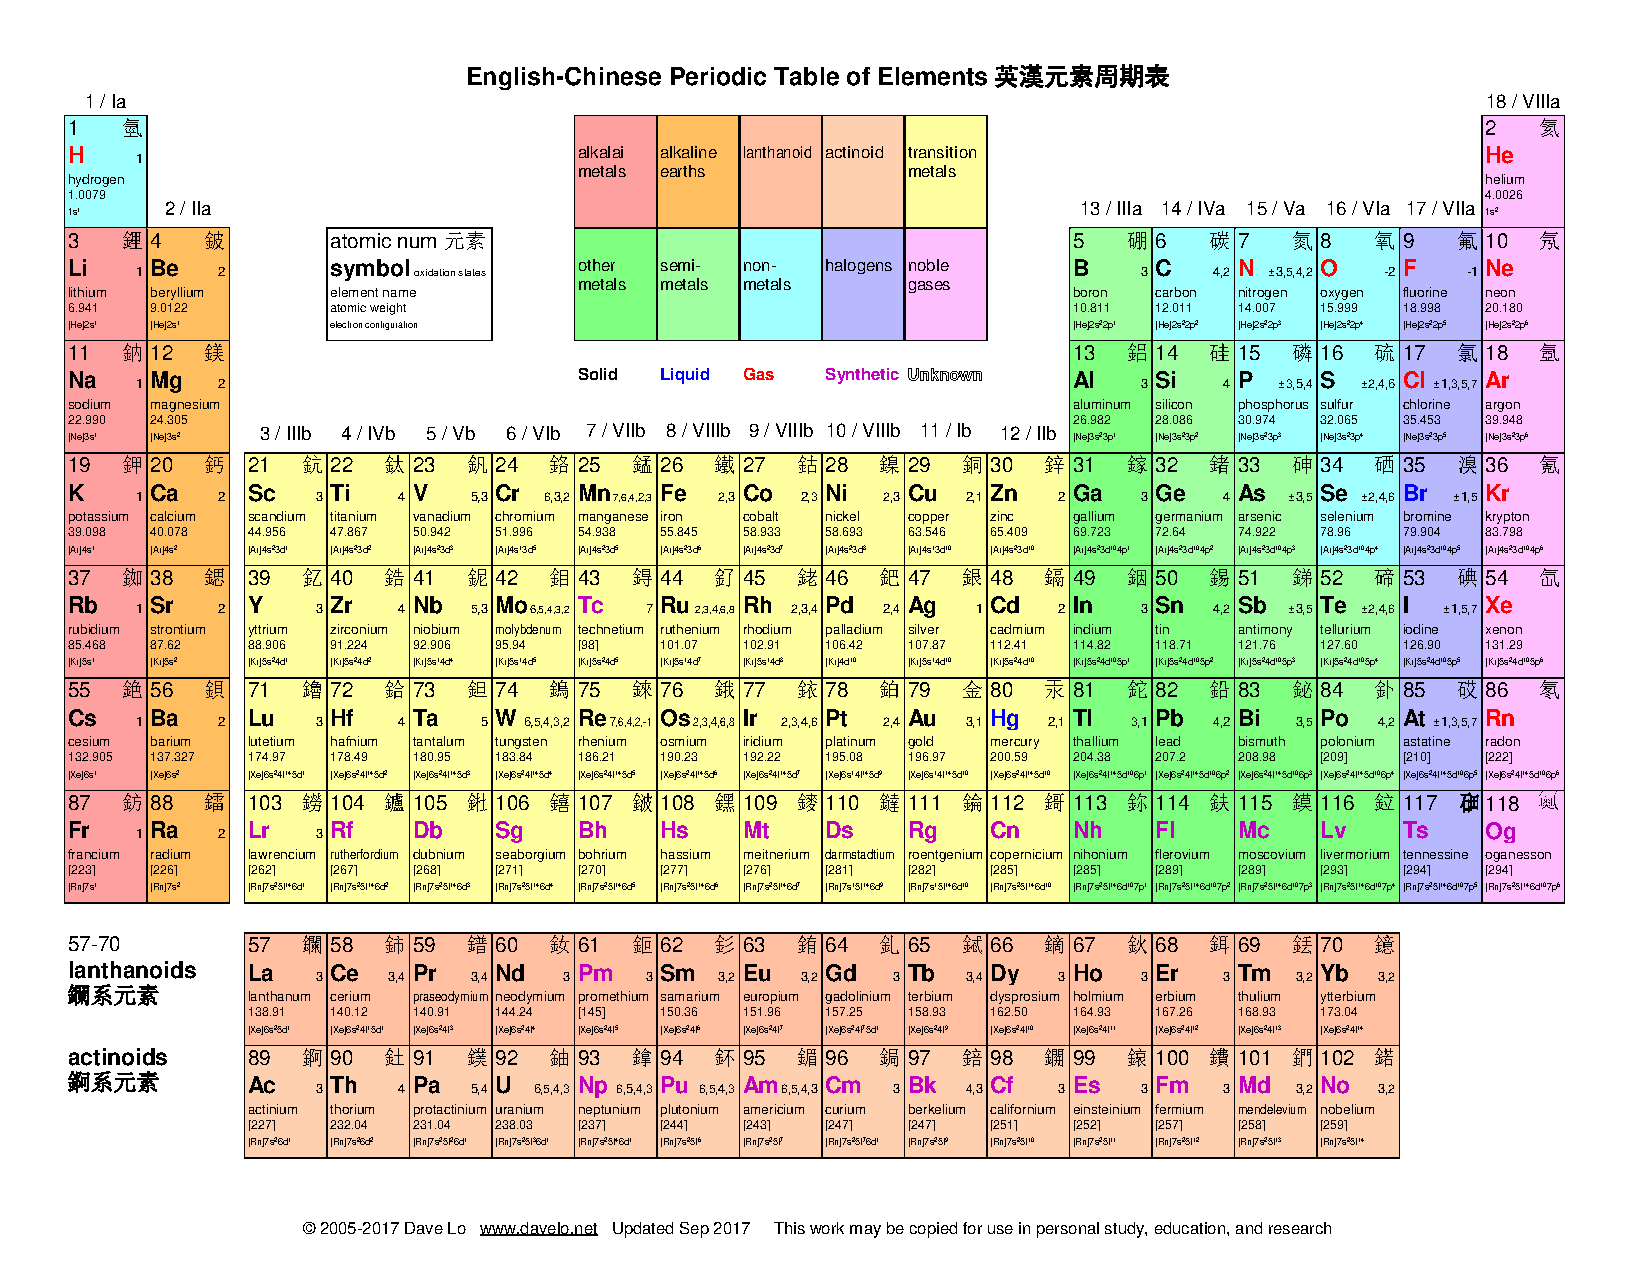
\includepdf[pages=-]{periodic_table_tra.pdf}


%%% Local Variables:
%%% mode: latex
%%% TeX-master: "main"
%%% End:


% References before Appendix.
\printbibliography[heading=bibintoc,title={Reference}]{}

% Prefer `appendices' environment over `appendix' command.
\begin{appendices}

\chapter{Long Code Line}
\label{cha:long-code-line}

\section{Appendix Notes}
\label{cha:appendix-notes}

The \textit{appendix} package provides \textit{appendices}
environment that renames each chapter to Appendix A, Appendix B,
etc. Similarly, sections are renamed to A.1, A.2,
etc. respectively.

\section{Embedded fonts in PDF}
\label{sec:pdffonts}

Here is an example of PDF file generated by \LaTeX{}. We use
command tool \textit{pdffonts} to examine embedded fonts:

\begin{lstlisting}[language={},caption={\LaTeX{} 内嵌字体},label={pdffonts},frame={tb},basicstyle=\tiny\ttfamily,linewidth=.88\textwidth]
name                                 type              encoding         emb sub uni object ID
------------------------------------ ----------------- ---------------- --- --- --- ---------
TVICFK+Tinos                         CID TrueType      Identity-H       yes yes yes      5  0
XYTJRZ+AdobeSongStd-Light-Identity-H CID Type 0C       Identity-H       yes yes no       7  0
NJETOY+Tinos-Italic                  CID TrueType      Identity-H       yes yes yes      9  0
VMQFJA+Tinos-Bold                    CID TrueType      Identity-H       yes yes yes     15  0
ILVYSG+NotoSansHans-Bold-Identity-H  CID Type 0C       Identity-H       yes yes yes     20  0
HEDEEX+migu-1m-regular               CID TrueType      Identity-H       yes yes yes     50  0
KQTNVZ+CMSY10                        Type 1C           Builtin          yes yes no      55  0
\end{lstlisting}  

\section{pgfplotstable template}
\label{sec:pgfplotstable-template}

\begin{minipage}[tbp]{1.0\linewidth}
\begin{lstlisting}[language=TeX,caption={pgfplotstable
template},label={lst:pgfplotstable-template},basicstyle=\scriptsize\ttfamily,linewidth=\textwidth]
\begin{table}[tbp]
  \centering{} \pgfplotstabletypeset[ multicolumn names, % allows
  to have column header name col sep=comma, % the seperator in our
  .csv file
  display columns/0/.style={ % numbering starts at 0
    column name=$Ampere$, % header name of first column
    column type={S},string type % use siunitx for formatting
  }, display columns/1/.style={ column name=$Voltage$, column
    type={S},string type }, display columns/2/.style={ column
    name=$Energy$, column type={S},string type }, every head
  row/.style={ before row={\toprule}, % have a rule at top
    after row={ \si{\ampere} & \si{\volt} & \si{joule} \\ % the
      siunitx units seperated by & \midrule % rule under units
    } }, every last row/.style={ after row=\bottomrule % rule at
    bottom }, ]{pgfplotstable.csv} % filename/path to file
  \caption{Table automation from .csv file.}
  \label{table-automation-from-csv}
\end{table}
\end{lstlisting}    
\end{minipage}

\begin{minipage}[tbp]{1.0\linewidth}
\begin{lstlisting}[language=TeX,caption={pgfplots
template},label={lst:pgfplots-template},basicstyle=\tiny\ttfamily,linewidth=\textwidth]
\begin{figure}[!h]
  \centering
  \begin{tikzpicture}
    \begin{axis}[
      width = \linewidth, % Scale the plot to \linewidth
      grid = major, grid style = dashed,
      xlabel = Voltage $U$, ylabel = Currency $I$, % Set the labels
      x unit = \si{\volt}, y unit = \si{\ampere}, % Set the respective units
      % axis lines = left % only display the left and bottom axes
      legend style = { at = {(0.5,-0.2)}, anchor = north }, % Put
      the legend below the plot x tick label style = { rotate =
        90, anchor = east } %
      Display labels sideways ]
      % add a plot from table; you select the columns by using the
      % actual column header name in the .csv file
      \addplot table[x=value 1,y=value 2,col
      sep=comma]{pgfplots.csv}; \legend{$U$ - $I$}
      % add another plot
      \addplot {x^2 - 2*x + 1}; % add a tailing semicolon
      \addlegendentry{$x^2 - 2x + 1$} % use addlegendentry instead
      of legend
    \end{axis}
  \end{tikzpicture}
  \caption{pgfplots by table csv file}
  \label{fig:pgfplots-by-table-csv-file}
\end{figure}
\end{lstlisting}
\end{minipage}

\newpage{}
\listoffigures{}
\listoftables{}
\lstlistoflistings{}

\end{appendices}

%%% Local Variables:
%%% mode: latex
%%% TeX-master: "main"
%%% End:

\appendix

\chapter{Too Big to Fit}
\label{cha:too-big-fit}

\section{pdffonts}
\label{sec:pdffonts}

Here is an example of PDF file generated \LaTeX{}. We use
\textit{pdffonts} to examine embedded fonts:
  
\begin{landscape}
\begin{lstlisting}[language={},caption={\LaTeX{} 内嵌字体},frame={tb},label={pdffonts}]
name                                 type              encoding         emb sub uni object ID
------------------------------------ ----------------- ---------------- --- --- --- ---------
TVICFK+Tinos                         CID TrueType      Identity-H       yes yes yes      5  0
XYTJRZ+AdobeSongStd-Light-Identity-H CID Type 0C       Identity-H       yes yes no       7  0
NJETOY+Tinos-Italic                  CID TrueType      Identity-H       yes yes yes      9  0
VMQFJA+Tinos-Bold                    CID TrueType      Identity-H       yes yes yes     15  0
ILVYSG+NotoSansHans-Bold-Identity-H  CID Type 0C       Identity-H       yes yes yes     20  0
HEDEEX+migu-1m-regular               CID TrueType      Identity-H       yes yes yes     50  0
KQTNVZ+CMSY10                        Type 1C           Builtin          yes yes no      55  0
\end{lstlisting}  
\end{landscape}

%%% Local Variables:
%%% mode: latex
%%% TeX-master: "main"
%%% End:


\backmatter{}

\chapter{Postscript}
\label{cha:postscript}

This is the summary note pertaining to the book. This is the
summary note pertaining to the book. This is the summary note
pertaining to the book. This is the summary note pertaining to the
book.

%%% Local Variables:
%%% mode: latex
%%% TeX-master: "main"
%%% End:


\end{document}

%%% Local Variables:
%%% mode: latex
%%% TeX-master: t
%%% TeX-engine: xetex
%%% End:
